%%%%%%%%%%%%
% SETTINGS %
%%%%%%%%%%%%

%%%%%%%%%%%%%%%%%%%
% Thesis Settings %
%%%%%%%%%%%%%%%%%%%

\documentclass[a4paper,11pt,fleqn]{book}

\usepackage[T1]{fontenc}
\usepackage[utf8]{inputenc}
\usepackage[french,german,english]{babel}


%%%%%%%%%%%%%%%%%%%%%%%%%%%%%%%%%%%%%%%%%%%%%%%%%%%%%%%%%%%%%%%%%%%%%%%%%%%
% EDOC THESIS TEMPLATE: Variant 2.0 -> Utopia, Gabarrit A (lighter pages) %
%%%%%%%%%%%%%%%%%%%%%%%%%%%%%%%%%%%%%%%%%%%%%%%%%%%%%%%%%%%%%%%%%%%%%%%%%%%

% Utopia font-typesetting including mathematical formula compatible with
% newer TeX-Distributions (>2010)
\usepackage{fourier}

\setlength{\textwidth}{146.8mm} % = 210mm - 37mm - 26.2mm
\setlength{\oddsidemargin}{11.6mm} % 37mm - 1in (from hoffset)
\setlength{\evensidemargin}{0.8mm} % = 26.2mm - 1in (from hoffset)
\setlength{\topmargin}{-2.2mm} % = 0mm -1in + 23.2mm
\setlength{\textheight}{221.9mm} % = 297mm -29.5mm -31.6mm - 14mm (12 to accommodate footline with pagenumber)
\setlength{\headheight}{14pt}
\setlength{\parindent}{0pt}

\usepackage{setspace} % increase interline spacing slightly
\setstretch{1.1}

\makeatletter
% align all floating figures,tables, etc. to the top margin
\setlength{\@fptop}{0pt}
\makeatother


\usepackage{graphicx,xcolor}
\graphicspath{{images/}}

\usepackage{subfig}
\usepackage{booktabs}
\usepackage{lipsum}
\usepackage{microtype}
\usepackage{url}
\usepackage[final]{pdfpages}

\usepackage{fancyhdr}
\renewcommand{\sectionmark}[1]{\markright{\thesection\ #1}}
\pagestyle{fancy}
	\fancyhf{}
	\renewcommand{\headrulewidth}{0.4pt}
	\renewcommand{\footrulewidth}{0pt}
	\fancyhead[OR]{\bfseries \nouppercase{\rightmark}}
	\fancyhead[EL]{\bfseries \nouppercase{\leftmark}}
	\fancyfoot[EL,OR]{\thepage}
\fancypagestyle{plain}{
	\fancyhf{}
	\renewcommand{\headrulewidth}{0pt}
	\renewcommand{\footrulewidth}{0pt}
	\fancyfoot[EL,OR]{\thepage}}
\fancypagestyle{addpagenumbersforpdfimports}{
	\fancyhead{}
	\renewcommand{\headrulewidth}{0pt}
	\fancyfoot{}
	\fancyfoot[RO,LE]{\thepage}
}

\usepackage{listings}
\lstset{language=[LaTeX]Tex,tabsize=4, basicstyle=\scriptsize\ttfamily, showstringspaces=false, numbers=left, numberstyle=\tiny, numbersep=10pt, breaklines=true, breakautoindent=true, breakindent=10pt}

\usepackage{hyperref}
\hypersetup{pdfborder={0 0 0},
	colorlinks=true,
	linkcolor=black,
	citecolor=black,
	urlcolor=black}
\urlstyle{same}

\makeatletter
\def\cleardoublepage{\clearpage\if@twoside\ifodd\c@page\else
    \hbox{}
    \thispagestyle{empty}
    \newpage
    \if@twocolumn\hbox{}\newpage\fi\fi\fi}
\makeatother \clearpage{\pagestyle{plain}\cleardoublepage}


%%%%%%%%%%%%%%%%%%
% CHAPTER HEADER %
%%%%%%%%%%%%%%%%%%

\usepackage{color}
\usepackage{tikz}
\usepackage[explicit]{titlesec}
\newcommand*\chapterlabel{}
\titleformat{\chapter}[display]  % type (section,chapter,etc...) to vary,  shape (eg display-type)
	{\normalfont\bfseries\Huge} % format of the chapter
	{\gdef\chapterlabel{\thechapter\ }}     % the label
 	{0pt} % separation between label and chapter-title
 	  {\begin{tikzpicture}[remember picture, overlay]
    \node[yshift=-8cm] at (current page.north west)
      {\begin{tikzpicture}[remember picture, overlay]
        \draw[fill=black] (0,0) rectangle(35.5mm,15mm);
        \node[anchor=north east,yshift=-7.2cm,xshift=34mm,minimum height=30mm,inner sep=0mm] at (current page.north west)
        {\parbox[top][30mm][t]{15mm}{\raggedleft $\phantom{\textrm{l}}$\color{white}\chapterlabel}};  %the black l is just to get better base-line alingement
        \node[anchor=north west,yshift=-7.2cm,xshift=37mm,text width=\textwidth,minimum height=30mm,inner sep=0mm] at (current page.north west)
              {\parbox[top][30mm][t]{\textwidth}{\color{black}#1}};
      \end{tikzpicture}
      };
    \end{tikzpicture}
   \gdef\chapterlabel{}
    } % code before the title body

\titlespacing*{\chapter}{0pt}{50pt}{30pt}
\titlespacing*{\section}{0pt}{13.2pt}{*0}  % 13.2pt is line spacing for a text with 11pt font size
\titlespacing*{\subsection}{0pt}{13.2pt}{*0}
\titlespacing*{\subsubsection}{0pt}{13.2pt}{*0}

\newcounter{myparts}
\newcommand*\partlabel{}
\titleformat{\part}[display]  % type (section,chapter,etc...) to vary,  shape (eg display-type)
	{\normalfont\bfseries\Huge} % format of the part
	{\gdef\partlabel{\thepart\ }}     % the label
 	{0pt} % separation between label and part-title
 	  {\setlength{\unitlength}{20mm}
	  \addtocounter{myparts}{1}
	  \begin{tikzpicture}[remember picture,overlay]
    \node[anchor=north west,xshift=-65mm,yshift=-6.9cm-\value{myparts}*20mm] at (current page.north east) % for unknown reasons: 3mm missing -> 65 instead of 62
      {\begin{tikzpicture}[remember picture, overlay]
        \draw[fill=black] (0,0) rectangle(62mm,20mm);   % -\value{myparts}\unitlength
        \node[anchor=north west,yshift=-6.1cm-\value{myparts}*20mm,xshift=-60.5mm,minimum height=30mm,inner sep=0mm] at (current page.north east)
        {\parbox[top][30mm][t]{55mm}{\raggedright \color{white} \partlabel $\phantom{\textrm{l}}$}};  %the phantom l is just to get better base-line alingement
        \node[anchor=north east,yshift=-6.1cm-\value{myparts}*20mm,xshift=-63.5mm,text width=\textwidth,minimum height=30mm,inner sep=0mm] at (current page.north east)
              {\parbox[top][30mm][t]{\textwidth}{\raggedleft \color{black}#1}};
       \end{tikzpicture}
      };
     \end{tikzpicture}
    \gdef\partlabel{}
   } % code before the title body

%%%%%%%%%%%%%%%%%%%
% Custom Packages %
%%%%%%%%%%%%%%%%%%%

\usepackage{algorithm}
\usepackage{algpseudocode}
\usepackage[fleqn]{amsmath}
\usepackage{amsfonts}
\usepackage{amssymb}
\usepackage{amsthm}
\usepackage[titletoc, title, header]{appendix}
\usepackage{bm}
\usepackage{chngcntr}
\usepackage{imakeidx}
\usepackage{import}
\usepackage[acronyms,nopostdot,nonumberlist,nogroupskip,toc,sort=standard]{glossaries}
\usepackage{glossary-tree}
\usepackage{glossary-mcols}
\usepackage{mathrsfs}
\usepackage{pgf,tikz,pgfplots}
\usepackage{tabularx}
\usepackage{wrapfig}

\usepackage{pdflscape}
\usepackage{afterpage}

% Uncomment this to show the page geometry lines
%\usepackage[showframe]{geometry}

%%%%%%%%%%%%%%%%%%%
% Custom Snippets %
%%%%%%%%%%%%%%%%%%%

\newcommand{\dcone}{\mathcal{D}(\|D \cdot\|_1, x)}
\newcommand{\V}{\mathcal{V}}
\newcommand{\E}{\mathcal{E}}
\newcommand{\mean}[1]{\mathop{\overline{#1}}}
\newcommand{\comment}[1]{\texttt{(#1)}}
\newcommand{\redcomment}[1]{\textcolor{red}{#1}}
\newcommand{\polar}{^{\mathsf{o}}}
\newcommand{\etal}{\textit{et al.}}
\newcommand{\ie}{\textit{i.e.,}}

\DeclareUnicodeCharacter{00A0}{~}

\renewcommand{\quote}[3][.5\textwidth]{
    \hfill
    \begin{minipage}{#1}
        #2
        \begin{flushright}
            --- #3
        \end{flushright}
    \end{minipage}
    \vspace{2cm}
}

% glossaries
\newglossary[sbg]{symbol}{sbd}{sbn}{Symbols}
\makeglossaries{}
\makeindex[columns=2, title=Index, intoc]
\loadglsentries{head/acronyms}
\loadglsentries{head/symbols}

% ams
\newtheorem{theorem}{Theorem}[section]
\newtheorem{corollary}{Corollary}[theorem]
\newtheorem{lemma}[theorem]{Lemma}
\newtheorem{proposition}{Proposition}[section]

\theoremstyle{definition}
\newtheorem{definition}{Definition}[section]
\newtheorem{example}{Example}[section]

\theoremstyle{remark}
\newtheorem*{remark}{Remark}
\newtheorem*{claim}{Claim}


% pf2 package
\let\proof\relax
\let\endproof\relax
\let\qed\relax
\usepackage{pf2} % Must come after the previous 3 commands
\pflongindent

% tikz
\usetikzlibrary{arrows.meta}
\usetikzlibrary{calc}
\usetikzlibrary{graphs}
\usetikzlibrary{positioning}
\pgfplotsset{compat=1.14}


% epfl visual identity
\definecolor{epfl-rouge}{HTML}{FF0000}
\definecolor{epfl-groseille}{HTML}{B51F1F}
\definecolor{epfl-leman}{HTML}{00A79F}
\definecolor{epfl-canard}{HTML}{007480}
\definecolor{epfl-ardoise}{HTML}{413D3A}
\definecolor{epfl-perle}{HTML}{CAC7C7}

% appendices

%\AtBeginEnvironment{subappendices}{% Start of subappendices environment
%\chapter*{Appendices}
%\addcontentsline{toc}{chapter}{Appendices}
%\counterwithin{figure}{section}
%\counterwithin{table}{section}
%}

%\AtEndEnvironment{subappendices}{%% End of subappendices environment
%\counterwithout{figure}{section}
%\counterwithout{table}{section}
%}


%%%%%%%%%%%%%%%%%%%%
% HEAD: Book-Begin %
%%%%%%%%%%%%%%%%%%%%

\begin{document}

\frontmatter{}

\begin{titlepage}

\centering

\begin{figure}
	{\raggedright
\includegraphics[width=4cm]{images/epfl}}
\end{figure}

\vspace*{\fill}

\begin{minipage}{0.9\textwidth}
	\centering
	\huge
	On the optimal sampling design for the \acrlong{gtv} decoder: recovering piecewise-constant graph signals from a few vertex measurements
\end{minipage}

\vspace*{\fill}

by\\
{\large Rodrigo CERQUEIRA GONZALEZ PENA}\\

\vspace*{\fill}

Lausanne, Switzerland\\
2019

\end{titlepage}




\cleardoublepage{}
\thispagestyle{empty}

\clearpage
\vspace*{\fill}
\begin{center}
    \begin{minipage}{0.4\linewidth}
        \begin{flushleft}
            Quem me dera\\
            um mapa de tesouro\\
            que me leve a um velho baú\\
            cheio de mapas do tesouro\\
        \end{flushleft}
        \begin{flushright}
            --- Paulo Leminski
        \end{flushright}
    \end{minipage}%
\end{center}
\vfill
\chapter*{Acknowledgements}
\markboth{Acknowledgements}{Acknowledgements}
\addcontentsline{toc}{chapter}{Acknowledgements}

\vspace*{\fill}

First of all, I am grateful that Pierre Vandergheynst accepted me into his group (LTS2) and had the insight to propose a research topic that would keep me interested, and busy, for years. Thank you in particular for encouraging me to go to any conference I was drawn to, even if I had no work to present there.

\vspace*{\fill}

At LTS2, my colleagues could not have been more welcoming. Benjamin Ricaud and Xavier Bresson were fundamental in introducing me to research life. Andreas Loukas became the source for discussing theory, and the ideal partner for playing questionable, but heartfelt, Flight of the Conchords covers. Through ups and downs, the Ph.D. students of LTS2 developed a good sense of comradery. I will not disclose, however, how much of this development involved table football. Listing everyone from LTS2, and neighboring groups, who helped me go through my doctoral studies would fill most of this page, but I thank you all for the time we shared.

\vspace*{\fill}

Most of my Ph.D. was funded by the European Union's FP7-PEOPLE-2013-ITN program under grant agreement n\textsuperscript{o} 607290 SpaRTaN. While I do appreciate the money, I would like to mostly thank the \emph{people} from  SpaRTaN and its partner network, MacSeNet. We learned together and we laughed together, and I believe we are all better off for having met one another. Especial thanks go to everyone at the CVSSP at the University of Surrey and at the Fraunhofer IDMT for hosting me.

\vspace*{\fill}

Much to my family's fault, I consider a life in pursuit of education to be a noble endeavor. Often when surrounded by books I am transported back home. I know that being nine thousand kilometers apart is hard on us, so I appreciate your support. My grandfather, being an immigrant himself, told me upon my moving that I now ``belonged to the world''. I agree, but I also believe in visiting for some coffee and loud conversations around the table.

\vspace*{\fill}

Lastly, and most importantly, I would like to thank my wife and confidante extraordinaire, Anna. She was a published author years before me, but never bragged about it. Anna lifted my mood when I had a hard time putting thoughts to paper; she will probably continue doing so long after I forget what I wrote here. This work is dedicated to you.

\vspace*{\fill}

\emph{Lausanne, 30 September 2019 \hfill R.~C.~G.~P.}


%%%%%%%%%%%%%%%%%%%%
% ENGLISH abstract %
%%%%%%%%%%%%%%%%%%%%

\cleardoublepage{}
\chapter*{Abstract}
\addcontentsline{toc}{chapter}{Abstract/Résumé}

\vspace*{\fill}

Compressed Sensing teaches us that measurements can be traded for offline computation if the signal being sensed has a simple enough representation. Proper decoders can exactly recover the high-dimensional signal of interest from a lower-dimensional vector of that signal's observations. In graph domains --- like social, similarity, or interaction networks --- the relevant signals often have to do with the network's cluster structure. Partitioning a graph into different communities induces a piecewise-constant signal, an object that can be decoded via \acrfull{gtv} minimization even if it is not fully observed. In fact, assume that such a signal can only be accessed by querying vertices at random. Then, we could sensibly ask: what are the sampling probabilities that minimize the number of queries required for a successful \acrshort{gtv} recovery? This thesis is an attempt to answer this question through the study of the success conditions in \acrshort{gtv} minimization programs. I show that the recovery error in these programs undergoes a phase transition in terms of the number of measurements, with a threshold that explicitly depends on the vertex-sampling probabilities. It suffices to minimize this threshold to obtain an optimal sampling design. Yet, sampling optimally in practice has problems of its own. While numerical experiments reveal that it is important to focus on the places of the graph where the signal varies, implementing the optimal design without actually knowing the signal-to-be-sampled remains an open issue.

\vspace*{\fill}

\textbf{Keywords:} Total Variation, graph signal processing, community structure, piecewise-constant signal, convex optimization, $\ell_1$ minimization, analysis sparsity, representer theorem, minimum restricted eigenvalue, small ball method, inexact dual certificate, golfing scheme

\vfill

%%%%%%%%%%%%%%%%%%%
% FRENCH abstract %
%%%%%%%%%%%%%%%%%%%

\begin{otherlanguage}{french}
\chapter*{Résumé}

\vspace*{\fill}

L'Acquisition Comprimée nous enseigne qu'il est possible d'échanger des mesures contre du calcul hors-ligne tant que le signal mesuré a une représentation suffisamment simple. Des décodeurs appropriés peuvent récupérer exactement le signal d’intérêt de grande dimension à partir d’un vecteur de plus petite dimension contenant des observations de ce signal. Dans les domaines de graphes --- comme les réseaux sociaux, de similarité ou d'interaction ---, les signaux pertinents ont souvent à voir avec la structure des clusters du réseau. Le partitionnement d'un graphe en différentes communautés induit un signal constant par morceaux, un objet qui peut être décodé via la minimisation de la Variation Totale sur le Graphe (\acrshort{gtv}) même s'il n'est pas complètement observé. En fait, supposons qu'un tel signal ne soit accessible qu'en interrogeant des nœuds de manière aléatoire. Alors, nous pourrions raisonnablement demander: quelles sont les probabilités d’échantillonnage minimisant le nombre de requêtes nécessaires à une reconstruction \acrshort{gtv} réussie? Cette thèse tente de répondre à cette question en étudiant les conditions de réussite des programmes de minimisation \acrshort{gtv}. Je montre que l’erreur de reconstruction dans ces programmes subit une transition de phase en termes du nombre de mesures, avec un seuil qui dépend explicitement des probabilités d’échantillonnage des nœuds. Il suffit de minimiser ce seuil pour obtenir un plan d'échantillonnage optimal. Cependant, échantillonner optimalement dans la pratique pose des problèmes particuliers. Bien que les expériences numériques révèlent qu'il est important de se concentrer sur les endroits du graphe où le signal varie, la mise en œuvre du plan optimal sans connaître réellement le signal à échantillonner reste une question ouverte.

\vspace*{\fill}

\textbf{Mots clés:} Variation Totale, traitement du signal dans les graphes, structure de communauté, signal constant par morceaux, optimisation convexe, minimisation  $\ell_1$, \emph{analysis sparsity}, théorème du représentant, valeur propre restreinte minimale, \emph{small ball method}, \emph{inexact dual certificate}, \emph{golfing scheme}

\vfill

\end{otherlanguage}



\tableofcontents{}

\glsaddall{} % Add all glossary entries, even the ones not referenced
%\glsfindwidesttoplevelname{} % Find widest name automatically
\glssetwidest{ABCDEFGHIJK} % Manually set the widest name
\setglossarystyle{alttree}
%\setglossarystyle{mcoltreenoname}
\printglossary[type=acronym, title={List of Acronyms}]
\printglossary[type=symbol, title={List of Symbols}]

\listoffigures{}
\addcontentsline{toc}{chapter}{List of figures}

\listoftables{}
\addcontentsline{toc}{chapter}{List of tables}

% space before each new paragraph according to the template guidelines.
% (after titlepage and frontmatter to keep the table of contents lists short)
\setlength{\parskip}{1em}


%%%%%%%%%%%%%%%%%%%%%%%%%%%%%%%%%%%%
% MAIN: The chapters of the thesis %
%%%%%%%%%%%%%%%%%%%%%%%%%%%%%%%%%%%%

\mainmatter{}

\chapter{Introduction}\label{ch:intro}

\quote[0.625\textwidth]{Eventually everything connects - people, ideas, objects. The quality of the connections is the key to quality per se.}{Charles Eames}

How much do the votes of politicians reflect their party affiliations? Stokes writes that ``political parties are endemic to democracy''~\cite[p.245]{stokes1999}, so wondering about the empirical expression of party beliefs is important to diagnose issues in the democratic process. It helps inform the debate of whether political parties ``made modern democracy'', contributing to its responsiveness and realization of public good, or ``are an inextricable weed'' in democracy's garden, ``partial to their own conception of the good''~\cite[pp.263--264]{stokes1999}. In Switzerland, the National Council is one of the main stages of federal politics~\footnote{It is one of the two houses that form the Federal Assembly of Switzerland, the other being the Council of States.}. Since 1963, it has had a fixed number of seats (200) divided into shares proportional to each canton's percentage of the total population. Every four years the Swiss people elects a new council, the most recent of which has held office from 2015 to 2019. It is the 50th legislature since the foundation of the Swiss federation, in 1848. Figure \ref{fig:snc_photo_and_parties} displays a photo of the Council hall, next to a scatter plot of the National Councillors taking part in the 50th legislature, highlighting their party affiliations.
\begin{figure}[H]
    \centering
    \subfloat[The Council hall at the Federal Palace in Bern, Switzerland. \textcopyright \, 2006 \url{http://www.parlament.ch}]{
        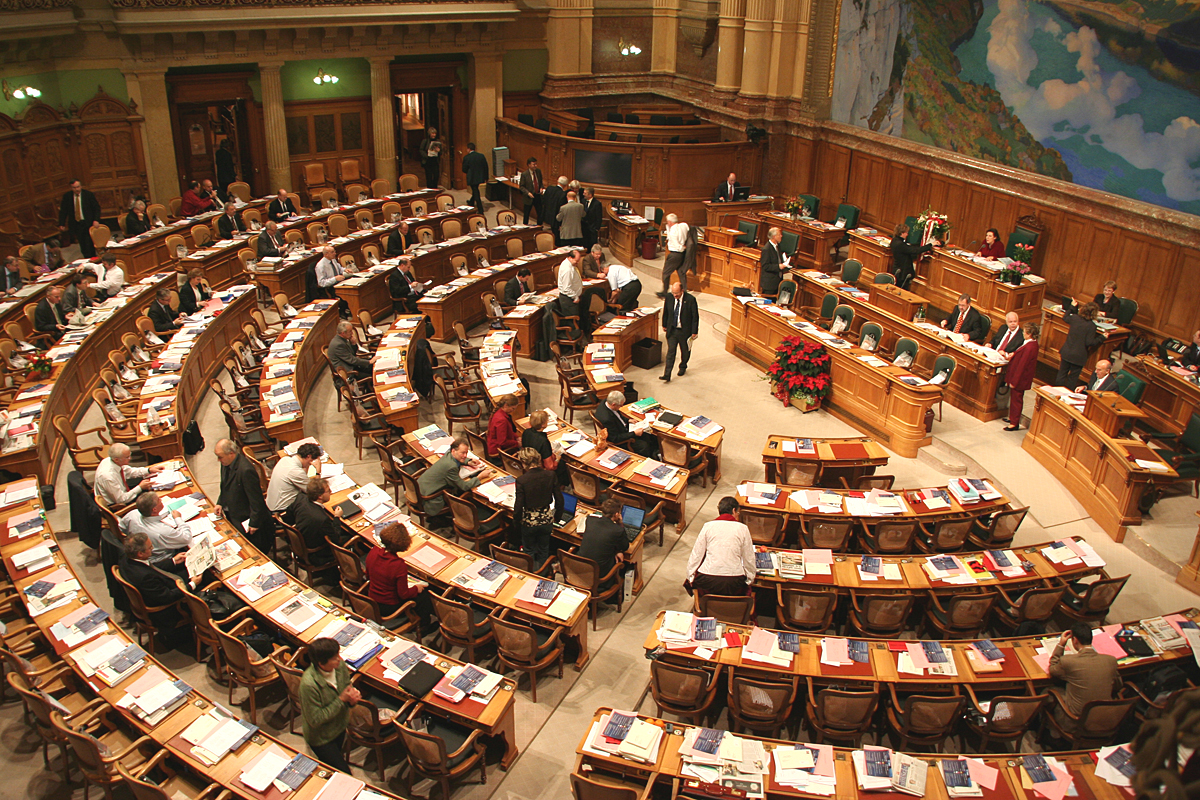
\includegraphics[width=0.5\textwidth]{snc_photo.jpg}
        \label{fig:snc_photo}
    }
    \hfill
    \subfloat[Council members and their party affiliations during the 50th legislature.]{
        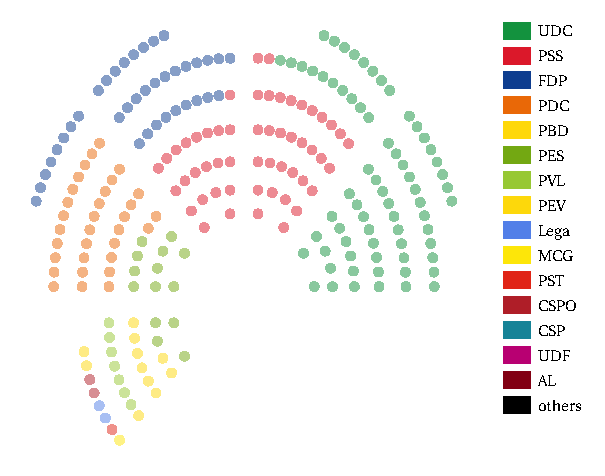
\includegraphics[width=0.45\textwidth]{snc_parties_no_edges.pdf}
        \label{fig:snc_parties_no_edges}
    }
    \caption[The Swiss National Council]{The Swiss National Council. The scatter plot on the right has more ``chairs'' than the 200 in the actual council hall on the left because I account for councillors that resigned or were replaced throughout the 50th legislature.}
    \label{fig:snc_photo_and_parties}
\end{figure}

The Swiss Parliament has an Open Data policy, allowing --- in particular --- the consultation of voting results through a database of parliamentary votes~\footnote{See \url{https://www.parlament.ch/en/ratsbetrieb/abstimmungen/abstimmungs-datenbank-nr}. I was pointed to this source by  D. Debruyn, Y. Morize, N. Orgland, and S. Stettler, who were all EPFL Master's students at the time.}. With this data, we can find out how each National Councillor voted in each of the affairs in the 50th legislature, and, comparing the voting patterns, record how similar the councillors are to one another in their voting behaviors. I depict these similarities in the form of a network (or graph) on Figure \ref{fig:snc_parties_with_edges}, with edges connecting councillors who voted the most alike during the period 2015--2019.~\footnote{I disclose the precise way in which this graph is constructed only in Chapter \ref{ch:numerical_tour}. For now, it suffices to interpret connected vertices as representing councillors with similar voting decisions.} Despite increasing polarization of the Council since the 1990s --- tied to the rise of the right-wing UDC party~\footnote{\url{https://www.swissinfo.ch/eng/political-drift_polarisation-of-swiss-parliament-continues/43752300}} --- it is not rare to find in Figure \ref{fig:snc_parties_with_edges} councillors from different parties that nonetheless vote alike. Had the Council been completely polarized, vertices of different colors would never connect. Still, party affiliation is not meaningless, as there seems to be more connections within than across parties. But how much of the party division in the Swiss National Council is encoded in the network structure induced by the voting data? Or, more concretely, if we knew the party affiliations of half the councillors, as in Figure \ref{fig:snc_subsampled_parties_with_edges}, could we infer the other half of the labels based on the connectivity information?

\begin{figure}[H]
    \centering
    \hfill
    \subfloat[The graph with all the party labels.]{
        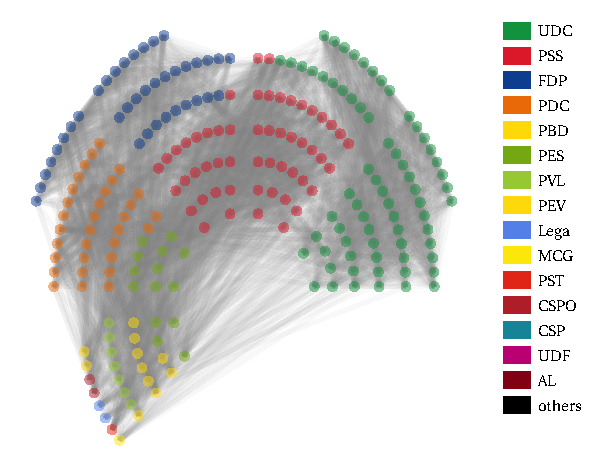
\includegraphics[width=0.45\textwidth]{snc_parties_with_edges.pdf}
        \label{fig:snc_parties_with_edges}
    }
    \hfill
    \subfloat[The graph with half the party labels.]{
        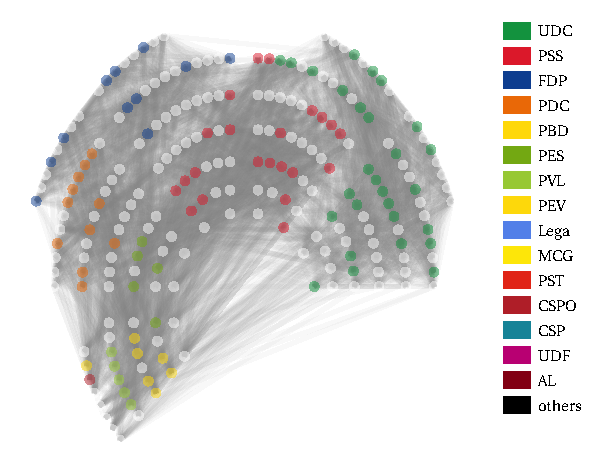
\includegraphics[width=0.45\textwidth]{snc_subsampled_parties_with_edges.pdf}
        \label{fig:snc_subsampled_parties_with_edges}
    }
    \hfill
    \caption[The voting-similarity graph for the Swiss National Council]{The voting-similarity graph for the Swiss National Council. Each vertex represents a council member, and the edges connect members that had similar voting patterns during the 50th legislature.}
\end{figure}

These musings are part of the usual pipeline in modern Data Science~\cite{vanderaalst2016}. An object of interest in the real-world (Swiss National Council) has some available data (vote results) that can be used to infer some property (party labels) of the object in question. The need for such inference may come from difficulties in measuring the desired property or simply out of scientific interest on the predictive powers of the available data. In the contrived example of the missing party labels in Figure \ref{fig:snc_subsampled_parties_with_edges}, we might be just interested to see if the voting patterns reflect the party affiliations. But in graphs such as the Internet or large social networks querying every single node for some property can be very expensive. The missing information in these cases is intrinsically due to the large size of the network. To infer, or recover, the full content from scarce observations, there are two main issues that practitioners concern themselves with. First, which kind of --- and how many --- measurements are available. Second, which machinery to use to retrieve the missing information. The first point pertains to what I call the \emph{sampling} stage of the pipeline; the second, to the \emph{decoding} stage. In this thesis, I assume the freedom to act in both, choosing a suitable decoder for an important class of signals, and subsequently looking for an optimal sampling strategy adapted to this decoder. Optimality here refers to reducing the number of measurements needed from the sampling stage for a successful decoding stage. An added benefit of studying optimal sampling lies in the possibility to quantify how suited the decoder is in retrieving the signals of interest. The more samples the decoder needs, the less suited it is. Take, for example, the Swiss National Council data, and imagine we chose a decoder for missing party labels (like those of Figure \ref{fig:snc_subsampled_parties_with_edges}) based on the voting-similarity connections. This decoder's optimal number of samples could therefore function as a numerical proxy to how well the councillors' votes echo their party affiliations.


\section{The main objects and questions in the thesis}

Networks (or graphs) have long been objects of interest in Mathematics and Computer Science, but they have found their way into Signal Processing over the last decade or so. \acrfull{gsp} is now an established subfield~\cite{shuman2013, sandryhaila2013a, ortega2018}, concerned with any quantities whose support can be interpreted as being a graph. As a matter of fact, I have already shown a graph signal. Each member (vertex) of the Swiss National Council  was associated with a party color, so we can understand the mapping ``councillor $\mapsto$ color'' in Figure \ref{fig:snc_subsampled_parties_with_edges} as a signal living on the voting-similarity graph. On the Internet, a relevant signal is the number of data packets at each router; on a social network, it might be people's likelihoods of buying a given product. Even when a graph is not naturally present --- as in the Swiss National Council example ---, representing the variable dependencies through a network may be a beneficial pre-processing step. To connect a vertex to only a few neighbors is akin to statistical selection, restricting a variable's predictors to its most similar peers. Moreover, these few connections implicitly constrain the interactions between vertices to happen only locally, so comparisons of signal values can be more efficiently computed.

One of the central tenets of \acrshort{gsp} can be stated as ``connected vertices have similar signal values''.~\footnote{An analogous statement, ``similar variables have similar outputs'', is the central assumption of the related field of Semi-Supervised Learning~\cite{chapelle2006}.} It is the glue that binds the graph and the signals that it supports, but it gives room to specify what ``similar values" means. This thesis deals with a particular set of graph signals deemed \emph{piecewise-constant}. In loose terms, these objects assume constant values over sizeable swathes of the graph, but are allowed to vary abruptly between the constant pieces. The councillors colors in Figure \ref{fig:snc_subsampled_parties_with_edges} is an example of piecewise-constant signal: each party defines a piece of constant color, but those colors are allowed to vary abruptly between pieces. In general, any classification or segmentation task can be interpreted as producing a piecewise-constant signal on some graph. Indeed, imagine a social network, then assign value $1$ to every person who has watched the 2010 movie ``The Social Network'', and value $0$ otherwise. The $\{0,1\}$-valued labels thus defined form a piecewise-constant signal over the social network. Whenever we know the value of a signal at a vertex of the graph, I will say that this vertex has been sampled. Sampled vertices represent the knowledge that an oracle made available to us to help us figure out the full underlying signal. This thesis admits oracles that provide \emph{vertex samples independently at random}, according to a probability distribution set beforehand. They are a model for any stakeholder that has a budget number of samples with which to query the network for a signal of interest. Some vertices may be more important than others, so they could be sampled them with higher likelihood; the samples are kept independent to facilitate the mathematical treatment of the process. Intuitively, if a company wants to sell a product, then ``influencers'' in a social network should definitely be queried for their propensity to advertise the merchandise. Readers will find in Chapter \ref{ch:graphs_signals_sampling} all the formalism that I use subsequent chapters when speaking of graphs, signals on graphs, and the sampling of these signals.

\begin{wrapfigure}{o}{0.35\textwidth}
    \centering
    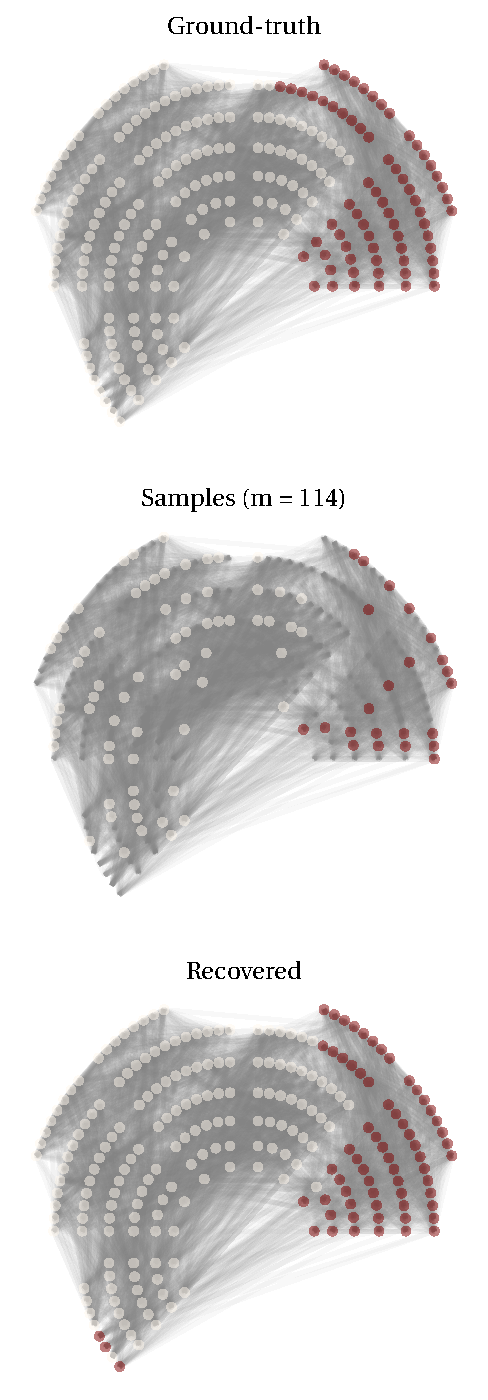
\includegraphics[width=0.3365\textwidth]{snc_sample_rec_example.pdf}
    \caption[The processing pipeline highlighting the sampling and decoding stages]{Example of the processing pipeline highlighting the sampling and decoding (recovery) stages. See the paragraph on the left for details.}
    \label{fig:snc_sample_rec_example}
\end{wrapfigure}

The decoders in this thesis manifest themselves in terms of \emph{convex programs}. That is, their output is chosen by minimizing some convex loss function. Piecewise-constant signals vary only across few of the edges on their graph support, so it makes sense to pair them with a recovery function that penalizes edge-differences.~\footnote{In a way, this recovery procedure is an instance of transductive learning \cite[Chapter 24]{chapelle2006} where the sampled vertices form the training set, the unsampled vertices the testing set, and the loss implicitly defines a search space.} This idea leads to the central subjects of the thesis, \acrfull{gtv} decoders. They are programs that minimize a semi-norm of the form $\|\mathbf{D} \cdot\|_1$, for some difference operator $\mathbf{D}$. \acrfull{tv} minimization is a standard tool for processing ``classic'' time-series or images that have rare, but sudden changes in value. Think here of a quantized waveform, or a Mondrian painting. I will show how \acrshort{tv} and piecewise-constant graph signals are also intimately related. Chapter \ref{ch:recovery_convex} provides the required background on convex recovery and introduces the \acrshort{gtv} decoders so central to this thesis.

The performance of the decoder depends on what happens at the sampling stage. To get a better feeling for this, let us revisit the Swiss National Council example, this time with a different graph signal. The top row of Figure \ref{fig:snc_sample_rec_example} depicts the indicator function of the Swiss People's Party (UDC in French), the largest party in the 50th legislature, occupying about 30\% of the total seats. The signal takes value $1$ (yellow) at vertices representing UDC members, and $0$ (blue) everywhere else. UDC is politically the farthest to the right on the National Council, so the party should be fairly well encoded in the voting patterns represented by the edges of the graph. In the middle row of Figure \ref{fig:snc_sample_rec_example}, I have sampled the UDC indicator function at 50\% of the vertices, uniformly at random. Many instances of both yellow (UDC) and blue (non-UDC) vertices appear in the sample because the party constitutes a considerable share of the Council. The third row of Figure \ref{fig:snc_sample_rec_example} shows the decoded signal as output by \acrshort{gtv} interpolation, yet to be introduced in Chapter \ref{ch:recovery_convex}. Most of the vertex labels are recovered correctly, but there are visibly wrong assignments. This means that sampling uniformly at random the labels of \emph{half} the councillors is still not enough to guarantee a perfect recovery using our decoder. Sampling uniformly at random, however, is not the only way to query the vertices under our oracle model. We could sample more often the vertices that are poorly connected, or sample more often the hubs of the graph, or even mix those two strategies. The possibilities are endless. Rather than think of an ad hoc plan of action, this thesis asks

\begin{center}
    \framebox[1.1\width][c]{%
        \parbox[t][44pt][c]{0.8\textwidth}{
            \centering
            What is the vertex sampling design that minimizes the number of measurements required for the success of \acrshort{gtv} decoders?
        }
}
\end{center}

The best hope one has to find a sampling design that answers the question above is by studying the conditions for successful recovery under \acrshort{gtv} minimization. In the course of this study, we will encounter typical concepts that usually arise when dealing with stochastic objects in high dimensions~\cite[Ch. 1]{vanhandel2014}, such as concentration, universality, and sharp transitions. In particular, I will show that the recovery error drops suddenly to zero (with a high likelihood) at a critical number of measurements that depends on the vertex sampling probabilities. Minimize this threshold and one can find the optimal sampling design.

\section{Contributions}

To prove that a convex program returns the desired output, one must produce a \emph{certificate}, an object whose very existence guarantees the success of the recovery procedure. Chapters \ref{ch:lower_bound_min_gain} and \ref{ch:inexact_dual} describe two parallel attempts that I made towards producing such guarantees.

In Chapter \ref{ch:lower_bound_min_gain}, the certificate manifests itself as a positive lower bound on a minimum gain functional. This view has proven fruitful when Gaussian-like vectors are used to measure the ground-truth signal, and has become standard in the literature~\cite{chandrasekaran2012, tropp2015a}. However the nature of vertex sampling gets in the way of the usual small-ball method~\cite{mendelson2015, koltchinskii2015} used to lower bound the minimum gain. As a result, I ultimately fail in this attempt, but I end the chapter pointing towards a possible redemption, reliant on better knowledge of the coordinate structure of a certain ``descent cone''.

The real win comes in Chapter \ref{ch:inexact_dual}, while seeking a \emph{dual} certificate for the \acrshort{gtv} decoder. There, the \acrlong{kkt} conditions of the problem motivate a blueprint for an iterative golfing scheme~\cite{gross2011} that produces, in the end, the desired recovery guarantee. It is this chapter that the number of measurements implying a successful recovery is upper bounded by an expression that depends on the vertex sampling probabilities. The optimal sampling design then comes directly as a corollary. Interestingly, the sampling probabilities in this design depend on how each vertex perturbs the graph difference operator, restricted to the edges across which the piecewise-constant, signal-to-be-recovered changes in value.

Chapter \ref{ch:numerical_tour} closes the thesis with a numerical tour to balance out the mostly theoretical discussion up to that point. There I plot --- for a variety of graphs and signals of interest ---, the phase transition undergone by the recovery error of a \acrshort{gtv} decoder when the number of sampled vertices changes. Experiments show how these phase transitions can be improved using proper sampling designs, but the question of how to make proper designs that  are also \emph{practical} remains open by the end of the book.

\section{The presentation of the proofs}

Most chapters in this thesis contain theorems with somewhat lengthy proofs, whose immediate presentation would disturb the flow of the text. For this reason, I have gathered detailed arguments largely in appendices at the end of the relevant chapters. The proofs themselves are written in a hierarchical structure, based on the guidelines of L. Lamport~\cite{lamport2012}. For the unfamiliar reader, this means that I build a sequence of discrete, provable claims leading to the desired result. Each of these discrete claims are settled as true either by appealing to established knowledge, or by presenting a sequence of discrete sub-claims. In the end, the full proof resembles a nested list. I have avoided too much nesting due to the obvious limitations of the printed format. Still, the hierarchical structure should make it easier to distill the arguments and find exactly where I use each assumption in the statement of their respective theorems.

\section{Reproducibility and Open Science}

\begin{minipage}{\textwidth}
    {%
    \setlength\intextsep{0pt}
        \begin{wrapfigure}{i}{0.15\textwidth}
            
\includegraphics[width=0.16\textwidth]{cc-by.png}
        \end{wrapfigure}
    %
    \noindent This work is licensed under a \href{http://creativecommons.org/licenses/by/4.0/}{Creative Commons Attribution 4.0 International License}. All the computer code required to reproduce the contents of this thesis is distributed under the \href{https://opensource.org/licenses/MIT}{MIT License}, and hosted at the following repository:
    %
    \begin{center}
        \framebox[1.1\width][c]{%
            \parbox[t][22pt][c]{0.5\textwidth}{\url{https://github.com/rodrigo-pena/phd-thesis}}
    }
    \end{center}%
    }
\end{minipage}

\chapter{Graphs, signals, and sampling}\label{ch:graphs_signals_sampling}

Graphs are combinatorial objects, but much of graph \emph{signal processing} is a matter of linear algebra. A real-valued signal supported on a network can be embedded on a Euclidean space with dimension equal to the number of vertices. In this space, various difference operators can be defined and used as a basis for Fourier analysis or dynamical process analogs for graph signals~\cite{shuman2013}.

The signals that this thesis cares about are piecewise-constant, a characteristic tantamount to having few variations (or jumps) in value across edges. To measure such variations, we work with an operator $\mathbf{D}$, called the graph gradient matrix, whose induced $p$-semi-norms $\|\mathbf{D} \cdot \|_p$ yield various ways to quantify the amount of signal variation on the graph. The semi-norms corresponding to $p = 1, 2$ receive special names: \acrfull{gtv} and Dirichlet form, respectively. The former is one of the main objects of study in the thesis; the latter appears sporadically, as a comparison point to the \acrshort{gtv}.

The act of sampling signal values is also cast in the language of linear algebra. Vertex measurements can be obtained through multiplication with a random matrix $\mathbf{A}$ indexed by a sampling set $\Omega$. Specifying the inclusion probabilities of indices into $\Omega$ is called a sampling design. This design is represented numerically by a vector $\bm{\pi}$, whose influence on the inclusion probabilities I present in two alternative ways, the \acrfull{ber} and \acrfull{cswr}. Convenience dictates which one is used when: \acrshort{ber} in Chapter \ref{ch:lower_bound_min_gain}; \acrshort{cswr} in Chapter \ref{ch:inexact_dual}. From the perspective of recovery problems, we will see that these two models are essentially equivalent.

This chapter's goal is to explain how the processing and sampling of graph signals can be seen as issues about vectors and matrices. Readers can use it as a reference because much of the notation in the thesis is already established here.


\section{Graph signal processing}

Graphs, or networks, are tuples $\mathcal{G} = (\V, \E)$ of a vertex set $\V$ and an edge set $\E$. The latter contains ordered pairs $e_{vu} = (v, u)$ that indicate directed connections from some vertex $v \in V$ to another vertex $u \in V$. We will consider a graph to be \textit{undirected} if $(v, u) \in \E \iff (v, u) \in \E$, that is, if vertex $v$ connects to $u$ if and only if $u$ also connects to $v$. Moreover, a graph has no \emph{self-loops} if $(v, v) \notin \E, \forall v \in \V$, and is \emph{connected} if, starting from any vertex, one can visit all the others by following the edges in $\E$. The graphs in the numerical examples of Chapter \ref{ch:numerical_tour} are all connected, undirected, and without self-loops. Any other reference to graphs in the rest of the text can be assumed to be valid for generic networks.

In machine learning and signal processing, graphs are commonly used to encode ``closeness'' or ``similarity'' between the objects represented by the vertices. A common way to quantify those similarities is by attaching non-negative weights to the edges of the graph. The larger the weight, the more similar the corresponding connected vertices. Formally, the weight assignment is done through a function $w : \E \to \mathbb{R}_{\ge 0}$. But an alternative representation of the weights can be derived once we impose an arbitrary ordering $v_1 < v_2 < \dots < v_n$ to the $n$ vertices in $\V$. With this fixed ordering, we can build a weighted adjacency matrix $\mathbf{W} \in \mathbb{R}^{n \times n}$ with entries given by

\begin{equation*}
    \forall i,j \in [n], \quad W_{ij} = \left \{
        \begin{matrix}
            w((v_i, v_j)) & \text{ if } (v_i, v_j) \in \E \\
            0 & \text{ otherwise}.
        \end{matrix}
    \right.
\end{equation*}

On undirected graphs, any pair $(v_i, v_j), (v_j, v_i)$ really represents the same undirected edge. In this case, we make the weight function symmetric, that is, $w((v_i, v_j)) = w((v_j, v_i))$, $\forall v_i, v_j \in \mathcal{V}$. As a consequence, $W$ for an undirected graph is a symmetric matrix. Whenever the weight function satisfies $w \equiv 1$, we say that the graph is unweighted, recovering in $W$ the classic adjacency matrix used in algebraic graph theory.

I reserve the variable $n$ for the number of vertices on a graph. In other words, for any $\mathcal{G} = (\V, \E)$, we will have $n := |\V|$. Alluding to the imposed order on the vertices of $\V$, we can employ a one-to-one mapping between $\V$ and $[n] := \{1, 2, \dots, n\}$. This mapping, takes $i \mapsto v_i$, and vice versa, for every $i \in [n]$. Without fear of ambiguity then --- and for the sake of presentation ---, I interchangeably refer to the vertex set as either $\V$ or $[n]$. Similarly, we keep the letter $N$ for referring to the number of edges, $|\E|$. The capital $N$ also works as a mnemonic device for the fact that the number of edges will almost always be larger than the number of vertices. In fact, for any connected, undirected graph $\mathcal{G}$, the bounds $|\V| - 1 \leq |\E| \leq \frac{|\V|(|\V| - 1)}{2}$ apply by a simple counting exercise. The lower bound is reached if $\mathcal{G}$ is a tree, whereas the upper bound holds whenever $\mathcal{G}$ is a complete graph.

Any function $f : \V \to \mathbb{R}^{n}$ is thought of as a signal on the graph. Intuitively, the naming is justified by imagining each vertex $v \in \V$ as having a real value $f(v)$ living on top of it. We can then refer to the graph as the support of the signal. This view is borrowed from graphs such as sensor networks, where each vertex (sensor) has a clear signal component (e.g., temperature) attached to it. But we can abstract from this example and refer to, say, the numerical labels of vertices in a clustered network as a graph signal as well.

For processing reasons, it is useful to identify the set of graph signals with the set of vectors in $\mathbb{R}^{n}$, via the bijection between $\V$ and $[n]$. In practice, this only means that for any $\mathbf{x} \in \mathbb{R}^{n}$ there exists a graph signal $f$ such that $\mathbf{x} = \left( f(v_i) \right)_{i = 1}^n$, for some ordering $v_1 < v_2 < \dots < v_n$ of the vertices in $\V$. From now on, having this identification in mind, I will only refer to graph signals as vectors in $\mathbb{R}^{n}$.

\begin{figure}[H]
    \centering
    \begin{tikzpicture}

    % axes
    %\draw[help lines, color=gray!30, dashed] (0,0) grid (12,7);

    % real axis
    \draw[-{Latex[length=3mm, width=3mm]}, very thick] (0,0) -- (0,5) node [right] {$\mathbb{R}$};
    \begin{scope}[every node/.style={anchor=east}]
        \node[color=epfl-perle] at (0,0) {$0$};
        \node[color=epfl-canard] at (0,2) {$1$};
        \node[color=epfl-groseille] at (0,4) {$2$};
    \end{scope}

    % vertices
    \begin{scope}[every node/.style={circle, thick, draw}]
        \node (v1) at (1,0.5) {$v_1$};
        \node (v2) at (2.5,2.5) {$v_2$};
        \node (v3) at (4.5,0.5) {$v_3$};
        \node (v4) at (6,2.5) {$v_4$};
    \end{scope}

    % edges
    \begin{scope}[every edge/.style={thick, draw}]
        \path (v1) edge (v2);
        \path (v2) edge (v3);
        \path (v3) edge (v4);
        \path (v3) edge (v1);
    \end{scope}

    % signal
    \begin{scope}[every node/.style={circle, fill},
                  every edge/.style={dashed, draw}]
        \node[color=epfl-groseille] (sv1) at (1,4.5) {};
        \node[color=epfl-groseille] (sv2) at (2.5,6.5) {};
        \node[color=epfl-groseille] (sv3) at (4.5,4.5) {};
        \node[color=epfl-canard] (sv4) at (6,4.5) {};

        \path[->, color=epfl-groseille] (v1) edge (sv1);
        \path[->, color=epfl-groseille] (v2) edge (sv2);
        \path[->, color=epfl-groseille] (v3) edge (sv3);
        \path[->, color=epfl-canard] (v4) edge (sv4);
    \end{scope}

    % level sets
    \fill[color=epfl-perle, fill=epfl-perle, fill opacity=0.2] (0,0) -- (2.25,3) -- (7,3) -- (4.75,0);
    \fill[color=epfl-canard, fill=epfl-canard, fill opacity=0.2] (0,2) -- (2.25,5) -- (7,5) -- (4.75,2);
    \fill[color=epfl-groseille, fill=epfl-groseille, fill opacity=0.2] (0,4) -- (2.25,7) -- (7,7) -- (4.75,4);

    % signal as a vector
    \node[anchor=center] (x) at (9.75, 4.5) {
        $
        \mathbf{x} = \left [
        \begin{matrix}
            \textcolor{epfl-groseille}{f(v_1)} \\
            \textcolor{epfl-groseille}{f(v_2)} \\
            \textcolor{epfl-groseille}{f(v_3)} \\
            \textcolor{epfl-canard}{f(v_4)}
        \end{matrix}
        \right ]
        = \left [
        \begin{matrix}
            \textcolor{epfl-groseille}{2} \\
            \textcolor{epfl-groseille}{2} \\
            \textcolor{epfl-groseille}{2} \\
            \textcolor{epfl-canard}{1}
        \end{matrix}
        \right ]
        \in \mathbb{R}^{4}
        $
    };

    % graph as a tuple
    \node[anchor=center] (g) at (9.75, 1.5) {
        $
        \begin{matrix}
            \mathcal{G} = (\mathcal{V}, \mathcal{E}) \\
            \mathcal{V} = \left\{ v_1, v_2, v_3, v_4 \right\} \\
            \mathcal{E} = \left\{ (v_1,v_2), (v_2,v_3), (v_3,v_4), (v_3,v_1), \right. \\
            \qquad \left. (v_2,v_1), (v_3,v_2), (v_4,v_3), (v_1,v_3) \right\}
        \end{matrix}
        $
    };

\end{tikzpicture}
    \caption[A signal supported on a graph]{A signal supported on a graph. The graph is a tuple $\mathcal{G} = (\mathcal{V}, \mathcal{E})$ of vertices and edges, and the signal is a function mapping vertices to the reals (in this case). The vector representation $\mathbf{x}$ of the graph signal gathers the function values at each vertex, once an (arbitrary) vertex ordering has been fixed.}
    \label{fig:graph-signal-example}
\end{figure}


\subsection{Piecewise-constant graph signals}\label{sec:piece_const_graph_signals}

In Figure \ref{fig:graph-signal-example} is what we would intuitively call a piecewise-constant signal: it assigns a constant value of $2$ for vertices $v_1, v_2, v_3$ and another constant value of $1$ to vertex $v_4$. We could even think that this signal encodes the community structure of this graph, with $v_1, v_2, v_3$ in one community and $v_4$ in another.

To properly define a signal that is constant by pieces, it helps to explore a notion of ``step-functions'' on graphs, similarly to how Figure \ref{fig:graph-signal-example} distinguishes between a ``red'' step and a ``blue'' step. The indicator vector of a subset $\mathcal{W} \subset \V$ is the object with entries
\begin{equation}
    \mathbb{1}_{\{ \mathcal{W} \}}[i] = \left \{
        \begin{matrix}
            1 & \text{if } v_i \in \mathcal{W} \\
            0 & \text{otherwise}
        \end{matrix}
    \right.
    , \enspace \forall i \in [n].
\end{equation}
The blue component of the signal in Figure \ref{fig:graph-signal-example} is the indicator vector of the vertex set $\{v_4\}$, while the red component is twice the indicator vector of $\{v_1, v_2, v_3\}$. Should we then state that any graph signal $\mathbf{x} \in \mathbb{R}^{n}$ is piecewise-constant if it can be written as a linear combination of indicator vectors? No, because the set of indicators $\left\{ \mathbb{1}_{\{ i \}} \right\}_{i=1}^n \equiv \{\mathbf{e}_i\}_{i=1}^n$ forms the standard basis in $\mathbb{R}^{n}$, so \emph{any} graph signal lies in its linear span. To earn the adjective of piecewise-constant, a signal must also have relatively few variations, which we can quantify with help from difference operators.


\subsection{Difference operators on graphs}\label{sec:diff_op_graphs}

The weights in the adjacency matrix $\mathbf{W}$ are supposed to represent how ``close'' vertices are to one another. Hence, it is natural to consider gradient maps $\nabla_{\mathcal{G}}f : \E \to \mathbb{R}^{N}$ of graph signals $f : \V \to \mathbb{R}^{n}$ as producing edge differences~\footnote{The square root in the expression is standard~\cite{shuman2013} and has to do with obtaining a clean expression for a related difference operator, the graph Laplacian.}
\begin{equation}
    (\nabla_{\mathcal{G}} f)[e] = \sqrt{\mathbf{W}_{j,i}} \left ( f(v_j) - f(v_i) \right ), \enspace \forall e = (v_i, v_j) \in \E.
\end{equation}
This gradient assigns each $e = (v_i, v_j)$ to a real number quantifying the variation of the signal $f$ from vertex $v_i$ to vertex $v_j$. If $f(v_j)$ is larger, this variation is positive, indicating that the signal \emph{increases} when going from $v_i$ to $v_j$.

As we have done for vertices, fix now an (arbitrary) ordering $e_1 < e_2 < \dots < e_N$ of the edges in $\E$. The gradient map can then be encoded in a weighted, signed, matrix $\mathbf{D} \in \mathbb{R}^{N \times n}$ with entries~\footnote{For readers familiar with graph theory, this is a version of the transpose incidence matrix.}
\begin{equation}
    \mathbf{D}_{kl} = \left \{
        \begin{matrix}
            \sqrt{\mathbf{W}_{ji}} & \text{if } l = i \\
            -\sqrt{\mathbf{W}_{ij}} & \text{if } l = j \\
            0 & \text{otherwise}
        \end{matrix}
    \right.,
    \quad \forall k \in [N], l \in [n], \text{ with } e_k = (v_i, v_j).
\end{equation}
If $\mathbf{x} = (f(v_i))_{i = 1}^n$ is the vector representation of a graph signal $f$, then the gradient map $\nabla_{\mathcal{G}} f$ can be just as well expressed by the matrix-vector multiplication $\mathbf{Dx}$. For this reason, I will refer to $\mathbf{D}$ as the gradient (or difference) operator associated with graph $\mathcal{G}$.

Going back to ``step functions'', one can verify that $\mathbf{D} \mathbb{1}_\mathcal{W}$ is supported~\footnote{The word ``support'' here refers to the edges corresponding to the non-zero entries of vector $\mathbf{D} \mathbb{1}_\mathcal{W}$.} on the boundary $\partial \mathcal{W} \subset \E$ corresponding to the edges between the vertex set $\mathcal{W}$ and its complement $\V \setminus \mathcal{W}$. In graph theory, $\partial \mathcal{W}$ is also known as the cut-set determined by the partition $(\mathcal{W}, \V \setminus \mathcal{W})$ of the vertex set.

We can use any $\ell_p$-norm to define a measure of ``size'' of a cut-set in a way that accounts for the edge weights:
\begin{align*}
    \left\| \mathbf{D} \mathbb{1}_{\{ \mathcal{W} \}} \right\|_p^p & = \sum_{e = (v_i,v_j) \in \E} \left( \mathbf{W}_{ji} \right)^{p/2} \left | \mathbb{1}_{\{ \mathcal{W} \}}[j] - \mathbb{1}_{\{ \mathcal{W} \}}[i] \right |^p \\
    & = \sum_{e = (i,j) \in \partial \mathcal{W}} \left( \mathbf{W}_{ji} \right)^{p/2}.
\end{align*}
The choice of $p$ only influences --- a priori --- the importance given to the edge weights for the size computation.

More generally, a linear combination of indicator vectors induces several partial cut-sets, one for each constant piece. I call the union of these partial cut-sets the \emph{jump-set}, indicating across which edges the signal changes value. For piecewise-constant graph signals, we should expect the size of the jump set to be small with respect to the total number $N$ of edges in the graph. The jump-set can be identified with an index set in $[N]$ via the action of $\mathbf{D}$.

\begin{definition}[Jump-set]
    The jump-set of a graph signal $\mathbf{x} \in \mathbb{R}^{n}$ is the set
    \begin{equation}
        \mathcal{S} := \operatorname{supp}\left ( \mathbf{Dx} \right )
    \end{equation}
    containing the indices of the non-zero entries of the weighted-edge-differences vector $\mathbf{Dx}$.
    \label{def:jump_set}
\end{definition}

\begin{figure}[H]
    \centering
    \begin{tikzpicture}

    % axes
    %\draw[help lines, color=gray!30, dashed] (0,0) grid (12,7);

    % real axis
    \draw[-{Latex[length=3mm, width=3mm]}, very thick] (0,0) -- (0,5) node [right] {$\mathbb{R}$};
    \begin{scope}[every node/.style={anchor=east}]
        \node[color=epfl-perle] at (0,0) {$0$};
        \node[color=epfl-canard] at (0,2) {$1$};
        \node[color=epfl-groseille] at (0,4) {$2$};
    \end{scope}

    % vertices
    \begin{scope}[every node/.style={circle, thick, draw}]
        \node (v1) at (1,0.5) {$v_1$};
        \node (v2) at (2.5,2.5) {$v_2$};
        \node (v3) at (4.5,0.5) {$v_3$};
        \node (v4) at (6,2.5) {$v_4$};
    \end{scope}

    % edges
    \begin{scope}[every edge/.style={thick, draw}]
        \path[<->] (v1) edge node[left] {$e_1$} node[right] {$e_2$} (v2);
        \path[<->] (v2) edge node[left] {$e_3$} node[right] {$e_4$}  (v3);
        \path[<->] (v3) edge node[left] {$e_5$} node[right] {$e_6$}  (v4);
        \path[<->] (v3) edge node[below] {$e_7$} node[above] {$e_8$}  (v1);
    \end{scope}

    % signal
    \begin{scope}[every node/.style={circle, fill},
                  every edge/.style={dashed, draw}]
        \node[color=epfl-groseille] (sv1) at (1,4.5) {};
        \node[color=epfl-groseille] (sv2) at (2.5,6.5) {};
        \node[color=epfl-groseille] (sv3) at (4.5,4.5) {};
        \node[color=epfl-canard] (sv4) at (6,4.5) {};

        \path[->, color=epfl-groseille] (v1) edge (sv1);
        \path[->, color=epfl-groseille] (v2) edge (sv2);
        \path[->, color=epfl-groseille] (v3) edge (sv3);
        \path[->, color=epfl-canard] (v4) edge (sv4);
    \end{scope}

    % level sets
    \fill[color=epfl-perle, fill=epfl-perle, fill opacity=0.2] (0,0) -- (2.25,3) -- (7,3) -- (4.75,0);
    %\fill[color=epfl-canard, fill=epfl-canard, fill opacity=0.2] (0,2) -- (2.25,5) -- (7,5) -- (4.75,2);
    %\fill[color=epfl-groseille, fill=epfl-groseille, fill opacity=0.2] (0,4) -- (2.25,7) -- (7,7) -- (4.75,4);

    % cutting plane
    \fill[color=epfl-ardoise, fill=epfl-ardoise, fill opacity=0.2] (3.5,3.5) -- (6.5,0.5) -- (6.5,3.5) -- (3.5,6.5);

    % difference signal as a vector
    \node[anchor=center] (Dx) at (9.75, 4.) {
        $
        \mathbf{Dx} = \left [
        \begin{matrix}
            \textcolor{epfl-groseille}{f(v_1)} - \textcolor{epfl-groseille}{f(v_2)}\\
            \textcolor{epfl-groseille}{f(v_2)} - \textcolor{epfl-groseille}{f(v_1)} \\
            \textcolor{epfl-groseille}{f(v_2)} - \textcolor{epfl-groseille}{f(v_3)} \\
            \textcolor{epfl-groseille}{f(v_3)} - \textcolor{epfl-groseille}{f(v_2)} \\
            \textcolor{epfl-groseille}{f(v_3)} - \textcolor{epfl-canard}{f(v_4)}\\
            \textcolor{epfl-canard}{f(v_4)} - \textcolor{epfl-groseille}{f(v_3)} \\
            \textcolor{epfl-groseille}{f(v_3)} - \textcolor{epfl-groseille}{f(v_1)} \\
            \textcolor{epfl-groseille}{f(v_1)} - \textcolor{epfl-groseille}{f(v_3)} \\
        \end{matrix}
        \right ]
        = \left [
        \begin{matrix}
            0 \\
            0 \\
            0 \\
            0 \\
            +1 \\
            -1 \\
            0 \\
            0 \\
        \end{matrix}
        \right ]
        $
    };

    % graph as a tuple
    \node[anchor=center] (S) at (9.75, 1.) {
        $
        \mathcal{S} := \operatorname{supp}\left ( \mathbf{Dx} \right) = \{5, 6\}
        $
    };

\end{tikzpicture}
    \caption[Difference operation on the graph signal]{Difference operation on the graph signal from Figure \ref{fig:graph-signal-example}, assuming unit-weight connections. The piecewise-constant signal varies only across two of the eight directed edges in the graph. The jump-set $\mathcal{S}$ indexes the twin edges $e_5$ and $e_6$, whose cut splits the graph into ``red'' and ``blue'' communities.}
    \label{fig:jump-set-example}
\end{figure}

We can also measure the size of the jump-set using $\ell_p$ norms of $\mathbf{Dx}$. Let $\mathbf{x} = \sum_{l=1}^{L} \alpha_l \mathbb{1}_{\{ \mathcal{W}_l \}}$ be a signal with $L$ constant pieces, taking values $\{ \alpha_l \}_{l=1}^{L}$ on corresponding disjoint vertex subsets $\mathcal{W}_1, \dots, \mathcal{W}_L$. The functional $\left \| \mathbf{D x} \right \|_p^p$ decomposes into $L$ terms, one for each constant piece:
\begin{align}
    \left \| \mathbf{D x} \right \|_p^p & = \sum_{e = (v_i,v_j) \in \E} \left(\mathbf{W}_{ji}\right)^{p/2} \left | \mathbf{x}[j] - \mathbf{x}[i] \right |^p \\
    & = \sum_{l=1}^{L} \sum_{v_i \in \mathcal{W}_l} \sum_{v_j \in \mathcal{W}_k \neq \mathcal{W}_l} \left(\mathbf{W}_{ji}\right)^{p/2} \left | \alpha_l - \alpha_k \right |^p. \nonumber
\end{align}
I give special names to the functionals corresponding to two particular choices of $p$.

\begin{definition}[\acrfull{gtv}]
    The \acrlong{gtv} of a signal $\mathbf{x} \in \mathbb{R}^{n}$ is given by
    \begin{equation}
        \left \| \mathbf{D x} \right \|_1 = \sum_{i \in [n]} \sum_{j \in [n]} \sqrt{\mathbf{W}_{ji}} \left | \mathbf{x}[j] - \mathbf{x}[i] \right |
    \end{equation}
    \label{def:gtv}
\end{definition}

\begin{definition}[Dirichlet form]
    The Dirichlet form of a signal $\mathbf{x} \in \mathbb{R}^{n}$ is given by
    \begin{equation}
        \left \| \mathbf{D x} \right \|_2^2 = \sum_{i \in [n]} \sum_{j \in [n]} \mathbf{W}_{ji} \left ( \mathbf{x}[j] - \mathbf{x}[i] \right )^2
    \end{equation}
    \label{def:dirichlet_form}
\end{definition}

\acrlong{gtv} is a constant presence in this thesis, whereas the Dirichlet form appears in chapters \ref{ch:recovery_convex} and \ref{ch:numerical_tour} as a comparison point for results concerning the \acrshort{gtv} semi-norm.

The null space of $\mathbf{D}$ is a particularly important object in the analysis of the \acrshort{gtv} decoders introduced in the next chapter. As usual for difference operators, $\operatorname{null} \left ( \mathbf{D} \right )$ is non-trivial, that is, it contains a subspace of dimension at least one. If the associated graph is \emph{connected}, this subspace is $\operatorname{span}(\mathbf{1})$, the set of \emph{constant} vectors in $\mathbb{R}^{n}$. If, however, the graph has \emph{disconnected} parts, then $\operatorname{null} \left ( \mathbf{D} \right )$ will also contain the vectors that are constant on each of the connected sub-graphs. In the limiting case of a graph without edges, $\operatorname{null} \left ( \mathbf{D} \right ) \equiv \mathbb{R}^{n}$.


\section{Sampling}\label{sec:sampling}

To sample is to request the values $f(v)$ for every vertex $v$ in some query set $\mathcal{Q} \subset \V$. In the vector interpretation of graph signals, this process is the same as measuring a coordinate subset of a point in $\mathbb{R}^{n}$. To sense coordinates, consider the standard basis $\left\{\mathbf{e}_i\right\}_{i=1}^n$ of $\mathbb{R}^{n}$, where each vector $\mathbf{e}_i$ contains a one at the $i$\textsuperscript{th} coordinate and zeros otherwise. Using this basis, a coordinate sample $y_i \in \mathbb{R}$ of a graph signal $\mathbf{x} = (f(v_i))_{i=1}^n$ at vertex $v_i$ is nothing but the inner product
\begin{equation*}
    y_i = \langle \mathbf{e}_i, \mathbf{x} \rangle = x_i.
\end{equation*}
More generally, given a sampling set $\Omega \in [n]$ of cardinality $|\Omega| = m$, we can form a matrix
\begin{equation}
    \mathbf{A} := \left( \mathbf{e}_i^\top \right)_{i \in \Omega} \in \mathbb{R}^{m \times n}
\end{equation}
and define a sampling vector $\mathbf{y} = (y_i)_{i=1}^n$ via the linear operation $\mathbf{y} = \mathbf{Ax}$.

Call $\mathbf{A} = \mathbf{A}(\Omega)$ the measurement matrix associated with the coordinate sampling set $\Omega$. Sometimes it will be convenient to ``lift'' the co-domain of $\mathbf{A}$ to $\mathbb{R}^{n}$, by inserting zero-valued rows for the coordinates outside the sampling set. The resulting square matrix is $\sum_{i \in \Omega} \mathbf{e}_i \mathbf{e}_i^\top =: \mathbf{P}_{\Omega}$, the orthogonal projection operator onto the sampling set. With that in mind, I will abuse notation every once in a while and write $\mathbf{A} = \mathbf{P}_{\Omega}$ as a shorthand.

A \emph{sampling design} is a blueprint for choosing $\Omega$, even if implicitly defined. In general, designs can be either deterministic or probabilistic, but we will consider only the latter~\footnote{Technically, it is possible to produce deterministic sampling designs from probabilistic ones by setting probability masses to either zero or one.}. I assign a numeric template to sampling design in the form of a vector $\bm{\pi} = (\pi_1, \pi_2, \dots, \pi_n)$. This vector assigns sampling probabilities to each element of $[n]$, but not necessarily their \emph{inclusion probabilities} into $\Omega$. Nonetheless, a larger $\pi_i$ implies a more likely sample of vertex $v_i$. We will assume that each coordinate is sampled \emph{independently} from the others, a convenient constraint for the probabilistic estimates in chapters \ref{ch:lower_bound_min_gain} and \ref{ch:inexact_dual}.

\begin{figure}[H]
    \centering
    \begin{tikzpicture}

    % axes
    %\draw[help lines, color=gray!30, dashed] (0,0) grid (12,7);

    % real axis
    \draw[-{Latex[length=3mm, width=3mm]}, very thick] (0,0) -- (0,5) node [right] {$\mathbb{R}$};
    \begin{scope}[every node/.style={anchor=east}]
        \node[color=epfl-perle] at (0,0) {$0$};
        \node[color=epfl-canard] at (0,2) {$1$};
        \node[color=epfl-groseille] at (0,4) {$2$};
    \end{scope}

    % vertices
    \begin{scope}[every node/.style={circle, thick, draw}]
        \node (v1) at (1,0.5) {$v_1$};
        \node (v2) at (2.5,2.5) {$v_2$};
        \node (v3) at (4.5,0.5) {$v_3$};
        \node (v4) at (6,2.5) {$v_4$};
    \end{scope}

    % edges
    \begin{scope}[every edge/.style={thick, draw}]
        \path (v1) edge (v2);
        \path (v2) edge (v3);
        \path (v3) edge (v4);
        \path (v3) edge (v1);
    \end{scope}

    % sampled vertices
    \begin{scope}[every node/.style={circle, fill},
                  every edge/.style={dashed, draw}]
        \node[color=epfl-groseille] (sv1) at (1,4.5) {};
        \node[color=epfl-canard] (sv4) at (6,4.5) {};

        \path[->, color=epfl-groseille] (v1) edge (sv1);
        \path[->, color=epfl-canard] (v4) edge (sv4);
    \end{scope}

    % unsampled vertices
    \begin{scope}[every edge/.style={dashed, draw}]
        \node (sv2) at (2.5,4.0) {?};
        \node (sv3) at (4.5,2.0) {?};

        \path[->] (v2) edge (sv2);
        \path[->] (v3) edge (sv3);
    \end{scope}

    % level sets
    \fill[color=epfl-perle, fill=epfl-perle, fill opacity=0.2] (0,0) -- (2.25,3) -- (7,3) -- (4.75,0);
    %\fill[color=epfl-canard, fill=epfl-canard, fill opacity=0.2] (0,2) -- (2.25,5) -- (7,5) -- (4.75,2);
    %\fill[color=epfl-groseille, fill=epfl-groseille, fill opacity=0.2] (0,4) -- (2.25,7) -- (7,7) -- (4.75,4);

    % sampled signal as a vector
    \node[anchor=center] (y) at (9.75, 3.5) {
        $
        \mathbf{y} = \left [
        \begin{matrix}
            \textcolor{epfl-groseille}{f(v_1)} \\
            \textcolor{epfl-canard}{f(v_4)}
        \end{matrix}
        \right ]
        =
        \underbrace{
        \left [
            \begin{matrix}
                1 & 0 & 0 & 0 \\
                0 & 0 & 0 & 1 \\
            \end{matrix}
        \right ]
        }_{\mathbf{A}}
        \mathbf{x}
        $
    };

    % graph as a tuple
    \node[anchor=center] (Omega) at (9.75, 1.) {$\Omega = \{v_1, v_4\}$};

\end{tikzpicture}
    \caption[Sampling the graph signal]{Sampling the graph signal of Figure \ref{fig:graph-signal-example}. A vertex is more likely to be in the sampling set $\Omega$ if its corresponding entry in $\bm{\pi} = \left( \pi_1, \pi_2, \pi_3, \pi_4 \right)$ is large. Vector $\mathbf{y}$ gathers the measured (sampled) signal values, a linear operation over the ground-truth $\mathbf{x}$.}
    \label{fig:sampling-graph-signal-example}
\end{figure}

There exist parametric possibilities for modeling the probabilities in $\bm{\pi}$. For an example, Jung \cite{jung2018} takes each $\pi_i$ from an exponential family, parametrized by the signal value $x_i$ at vertex $v_i$. We will proceed otherwise, seeing the entries of $\bm{\pi}$ merely as unspecified real numbers in the interval $[0,1]$.


\subsection{\texorpdfstring{\acrfull{ber}}{Bernoulli Sampling Model}}\label{sec:ber}

Define random selectors $\{ \delta_i \}_{i=1}^n$ by drawing $n$ independent, $\{0, 1\}$-valued Bernoulli random variables, each of which according to the probabilities
\begin{equation}
    \mathbb{P} \left ( \left \{  \delta_i = 1 \right \}\right ) = \pi_i = 1 - \mathbb{P} \left ( \left \{  \delta_i = 0 \right \}\right ), \forall i \in [n].
\end{equation}
These selectors induce a sampling set according to the rule $\Omega = \{ i \in [n] : \delta_i = 1\}$. Note that each vertex $i \in [n]$ is \emph{included} in the sampling set with probability
\begin{equation*}
    \mathbb{P} \left ( \left \{  i \in \Omega \right \}\right ) = \pi_i.
\end{equation*}

An advantage of using Bernoulli selectors is that the independent coordinate samples \emph{do not repeat}. There is no redundancy in the sampling set, in the sense that the number of unique coordinate observations is equal to the cardinality of $\Omega$. The downside is that this cardinality is itself a \emph{random variable}. Indeed, $|\Omega| = \sum_{i=1}^{n} \delta_i$, so the number of samples is not determined a priori. Fortunately, the distribution $|\Omega|$ is fairly well concentrated around its expectation $\mean{m} := \mathbb{E} \left ( |\Omega| \right ) = \sum_{i=1}^{n} \pi_i$. An application of the scalar Bernstein inequality (Lemma \ref{lem:scalar_bern}) yields
\begin{equation}
    \frac{\mean{m}}{2} \leq |\Omega| \leq \frac{3 \mean{m}}{2},
\end{equation}
with probability at least $1 - 2 \exp \left ( -  \mean{m} / 9 \right )$.

The (lifted) measurement matrix induced from the Bernoulli model can be written directly in terms of the selectors, bypassing the sampling set $\Omega$:
\begin{align}
    \mathbf{A} = \sum_{i \in \Omega} \mathbf{e}_i^\top \mathbf{e}_i^\top = \sum_{i=1}^n \delta_i \mathbf{e}_i^\top \mathbf{e}_i^\top,
\end{align}
this expression will be very useful in Chapter \ref{ch:lower_bound_min_gain}.


\subsection{\texorpdfstring{\acrfull{cswr}}{Coordinate Sampling with Replacement}}\label{sec:cswr}

Let $\omega$ be a random variable taking values in $[n]$ with probabilities $\mathbb{P} \left ( \left \{ \omega = i \right \}\right ) = \pi_i$, for each $i \in [n]$. Draw $m$ \acrshort{iid} copies, $\omega_1, \omega_2, \dots, \omega_m$, of $\omega$ and define the sampling \emph{multiset} $\Omega = \{ \omega_i \}_{i=1}^m$ containing all those copies, including repetitions. This process effectively implements independent coordinate sampling with replacement. In particular, setting $\pi = (1/n, \dots, 1/n)$, one retrieves uniform random sampling.

Compared to the Bernoulli model, the likelihood that any given vertex $i \in [n]$ is in the sampling set has a more complicated expression:
\begin{align*}
    \mathbb{P} \left ( \left \{ i \in \Omega \right \}\right ) & = \mathbb{P} \left ( \left \{  \omega_1 = i \vee \dots \vee \omega_m = i \right \}\right ) \\
    & = 1 - \mathbb{P} \left ( \left \{  \omega_1 \neq i \wedge \dots \wedge \omega_m \neq i \right \}\right ) \\
    & = 1 - \mathbb{P} \left ( \left \{ \omega \neq i \right \}\right )^m \enspace \comment{\acrshort{iid}}\\
    & = 1 - (1 - \pi_i)^m.
\end{align*}
However, the total number of measurements is now deterministic and equal to $m$. This property proves to be convenient in Chapter \ref{ch:inexact_dual}.


\subsection{Reconstruction from samples}

Behind every sampling procedure, there is an underlying signal $\mathbf{x}$ which is the real object of interest. Sometimes the measurements only need to be numerous enough to estimate the mean, variance or other simple statistics of $\mathbf{x}$. We, however, want to recover the \emph{full} signal, in the spirit of \acrfull{cs}.

It should be expected that our ability to reconstruct a sub-sampled signal depends on how many measurements we have taken. If we sample all of the $n$ coordinates of $\mathbf{x}$ then the problem is trivially solved; if we sample none, there is no hope for recovery. The interesting cases are somewhere in between, especially when the number of measurements $m$ is much smaller than the dimension $n$ of the signal, a setup we informally refer to as $m \ll n$. In terms of linear algebra, recovery of $\mathbf{x}$ from $\mathbf{y} = \mathbf{Ax}$ is an attempt to invert a matrix $\mathbf{A} \in \mathbb{R}^{m \times n}$ that is rank-deficient. This problem has infinitely many solutions and is therefore ill-posed. In Chapter \ref{ch:recovery_convex}, I present decoders $\mathfrak{D} : \mathbb{R}^{m} \to \mathbb{R}^{n}$, based on convex optimization, that remedy this situation. They revert the measurement process, yielding $\mathbf{x} = \mathfrak{D}(\mathbf{y})$, as long as $\mathbf{x}$ belongs to a restricted class of vectors within $\mathbb{R}^{n}$.

I have previously postulated that the optimal sampling design for a fixed decoder will minimize the number of measurements needed for a successful recovery. Intuitively, such a design should sample more often the coordinates that contribute the most to the recovery confidence, while neglecting those that do not add as much value. In terms of the probabilities in $\bm{\pi} = (\pi_1, \dots, \pi_n)$, each entry $\pi_i$ can be thus seen as an importance measure of coordinate $i$ from the perspective of the decoder. These guidelines become formal once we can precise how each of the sampling probabilities in $\bm{\pi}$ affects the performance of the decoder.


\subsection{``Equivalence'' between the sampling models}\label{sec:samp_equiv}

Using the \acrshort{ber} or the \acrshort{cswr} model in our context is essentially a matter of convenience. Indeed, we can borrow an argument by Cand\`es \etal~\cite[Appendix]{candes2011a}, which I have detailed in Appendix \ref{ap:proof_equiv}. The reasoning holds in the context of any decoder whose success probability, $\mathbb{P} \left ( \left \{ \text{Success} \right \}\right )$, is monotonically increasing with the sample size $m$. This is the case for the procedures commonly used in \acrlong{cs}.

To begin, $\mathbb{P} \left ( \left \{ \text{Success} \right \}\right )$ when sampling \emph{without} replacement can only be larger than the corresponding success probability when sampling \emph{with} replacement when we have the same number of measurements in both settings. The \acrshort{ber} model is without replacement, but produces a \emph{random} number of measurements. The tails of this distribution allow the redundant \acrshort{cswr} model to ``catch-up'', as long as the number of redundant samples in the latter is slightly larger than the average produced by \acrshort{ber}. Ultimately the two models, \acrshort{cswr} and \acrshort{ber}, need a similar number of measurements to reach the same recovery success probability.

A related discussion comparing the use of sampling with or without replacement can be found in Gross and Nesme~\cite{gross2010}, grounded on a classical moment domination result by Hoeffding \cite{hoeffding1963}.


\section{Summary}

We can reason about signal processing on graphs by defining appropriate vector spaces and linear operators therein that depend on the connections between vertices. Fundamentally, signal variations across edges can be measured a map $\mathbf{x} \mapsto \mathbf{Dx}$. Piecewise-constant graph signals are the ones that have few edge variations, or a ``small'' jump-set. The size of the jump-set can be measured by $\ell_p$ semi-norms induced by the graph gradient operator, allowing us to assess the degree to which a signal can be deemed piecewise-constant. Table \ref{tab:concepts-graph-gradient} is a record of important Graph Signal Processing objects that are often referenced in the following chapters.

\begin{table}[H]
    \begin{center}
        \begin{tabular}{ l l }
            \hline\noalign{\smallskip}
            Concept & Notes \\[.1cm]
            \hline\noalign{\smallskip}
            Number of vertices & $n$ \\[.25cm]
            Number of edges & $N$ \\[.25cm]
            Jump-set of a signal $\mathbf{x}$ & $\mathcal{S} := \operatorname{supp}\left ( \mathbf{Dx} \right )$ \\[.25cm]
            $\operatorname{null} \left ( \mathbf{D} \right )$ & Contains at least $\operatorname{span}(\mathbf{1})$ \\[.25cm]
            \acrfull{gtv} & $\| \mathbf{Dx} \|_1 = \sum_{i,j} \sqrt{\mathbf{W}_{ji}} \left | \mathbf{x}[j] - \mathbf{x}[i] \right |$\\[.25cm]
            Dirichlet form & $\| \mathbf{Dx} \|_2^2 = \sum_{i,j} \mathbf{W}_{ji} \left ( \mathbf{x}[j] - \mathbf{x}[i] \right )^2$\\[.1cm]
            \hline
        \end{tabular}
    \end{center}
    \caption[Summary of objects related to the graph gradient operator]{Summary of objects related to the graph gradient operator $\mathbf{D} \in \mathbb{R}^{N \times n}$.}
    \label{tab:concepts-graph-gradient}
\end{table}

Vertex sampling is also a linear operation, $\mathbf{x} \mapsto \mathbf{Ax}$, where the rows of $\mathbf{A}$ are taken from the standard basis of $\mathbb{R}^{n}$, indexed by a sampling set $\Omega \subset [n]$. A sampling design is a choice of a vector $\bm{\pi} = (\pi_i, \dots, \pi_n)$ that determines the inclusion probabilities of elements of $[n]$ into $\Omega$. I introduced two models for independent random sampling, named \acrshort{ber} and \acrshort{cswr}, that are almost equivalent in the context of recovery problems. Their use in chapters \ref{ch:lower_bound_min_gain} and \ref{ch:inexact_dual}, respectively, is dictated by convenience. Table \ref{tab:sampling-models} is a reference point for some properties of these two sampling models.

\begin{table}[H]
    \begin{center}
        \begin{tabular}{ l l l l }
            \hline\noalign{\smallskip}
            Model & Rows of $\mathbf{A}$ & Repeated samples & Number of samples ($|\Omega|$) \\[.1cm]
            \hline\noalign{\smallskip}
            \acrshort{ber} & drawn independently & no & $m \in \left[ \frac{1}{2}\bm{\pi}^{\top} \mathbf{1}, \frac{3}{2}\bm{\pi}^{\top} \mathbf{1} \right ]$ \acrshort{whp} \\[.25cm]
            \acrshort{cswr} & drawn independently & yes & $m$ deterministic \\[.1cm]
            \hline
        \end{tabular}
    \end{center}
    \caption[Summary of sampling models]{Summary of sampling models used to construct the measurement matrix $\mathbf{A}$ from a random (multi-)set of integers $\Omega \subset [n]$.}
    \label{tab:sampling-models}
\end{table}

\clearpage

\begin{subappendices}
    \section{``Equivalence'' of sampling models}\label{ap:proof_equiv}
    This appendix adapts reasoning found in \cite[Appendix]{candes2011a}, arguing for a certain equivalence between the sampling models introduced in Section \ref{sec:sampling}. For the purposes of the sort of decoders used in this thesis, a recovery guarantee obtained from one sampling model automatically implies a similar recovery guarantee for the other.

Assume we have an algorithm that takes as input coordinate samples of some $n$-dimensional vector and outputs a vector in $\mathbb{R}^{n}$. Denote by $\texttt{Success}$ the event whereby this algorithm produces the correct output. The notion of success can be arbitrary, as long as its probability never decreases as the number of samples increases. In other words, if the samples are indexed by a random set $\Omega$, the quantity $\mathbb{P} \left ( \left \{ \texttt{Success} \right \}\right )$ is monotonically increasing with increasing $\mathbb{E} |\Omega|$.

Now, denote by $\mathbb{P}_{\text{\acrshort{ber}}} \left ( \left \{  \texttt{Success} \right \}\right )$ and $\mathbb{P}_{\text{\acrshort{cswr}}} \left ( \left \{  \texttt{Success} \right \}\right )$ the probabilities of success induced by the distributions of the \acrfull{ber} and the \acrfull{cswr}, respectively. Recall that \acrshort{cswr} always draws $m$ samples, while the number of samples produced by \acrshort{ber} is random, with mean denoted by $\mean{m} = \mathbb{E} \left ( |\Omega| \right )$. For any fixed sampling design $\bm{\pi}$, I will put the number of samples in evidence by referring to the \acrlong{ber} as Ber($\mean{m}$) and to the \acrlong{cswr} as CSWR($m$).\footnote{The design $\bm{\pi}$ is fixed only up to a normalizing constant, because $\bm{\pi}^\top \mathbf{1} = 1$ for the \acrshort{cswr} model, whereas this need not hold for \acrshort{ber}.}

\begin{lemma}
    Let $\mean{m} = \frac{1}{1 + \varepsilon} m$, for any $\varepsilon > 0$. Then, a success probability of $P$ under CSWR($m$) implies a success probability of $P \left [ 1 - 2 \exp \left ( \frac{-3 \varepsilon \mean{m}}{8} \right ) \right ]$ under Ber($\mean{m}$) .
\end{lemma}

\begin{proof*}
    \mainproof

    \pf
    \step{}{
        A direct calculation reveals
        \begin{align*}
            \mathbb{P}_{\text{Ber}(\mean{m})} \left ( \left \{  \texttt{Success} \right \}\right ) & \geq \sum_{k=m}^{n} \mathbb{P}_{\text{Ber}(\mean{m})} \left ( \left \{  \texttt{Success} | |\Omega| = k \right \} \right ) \mathbb{P}_{\text{Ber}(\mean{m})} \left ( \left \{ |\Omega| = k \right \} \right ) \\
            & \geq \mathbb{P}_{\text{CSWR}(m)} \left ( \left \{  \texttt{Success} \right \} \right ) \sum_{k=m}^{n} \mathbb{P}_{\text{Ber}(\mean{m})} \left ( \left \{  |\Omega| = k \right \}\right ) \\
            & = \mathbb{P}_{\text{CSWR}(m)} \left ( \left \{  \texttt{Success} \right \} \right ) \mathbb{P}_{\text{Ber}(\mean{m})} \left ( \left \{ |\Omega| \geq m \right \} \right ) \\
            & = \mathbb{P}_{\text{CSWR}(m)} \left ( \left \{ \texttt{Success} \right \} \right ) \left [ 1 - \mathbb{P}_{\text{Ber}(\mean{m})} \left ( \left \{  |\Omega| < c\mean{m} \right \}\right ) \right ] \\
            & \geq \mathbb{P}_{\text{CSWR}(m)} \left ( \left \{ \texttt{Success} \right \} \right ) \left [ 1 - 2 \exp \left ( -3 c\mean{m} / 8 \right ) \right ]
        \end{align*}
    }
    \begin{proof} \pf
        \step{}{
            Conditioned on its cardinality, the distribution of $\Omega$ under Ber($\mean{m}$) is equivalent to coordinate sampling \emph{without} replacement. A sample without replacement always implies more distinct elements in $\Omega$ than a sample with replacement (for the same number of measurements). Thus, for any $k \geq m$,
            \begin{equation*}
                \mathbb{P}_{\text{Ber($\mean{m}$)}} \left ( \left \{ \texttt{Success} | |\Omega = k|\right \}\right ) \geq \mathbb{P}_{\text{CSWR($m$)}} \left ( \left \{  \texttt{Success} \right \}\right ).
            \end{equation*}
        }
        \step{}{
            The mononicity assumption also implies, for every $k \leq m$,
            \begin{equation*}
                \mathbb{P}_{\text{CSWR($k$)}} \left ( \left \{  \texttt{Success} \right \}\right ) \leq \mathbb{P}_{\text{CSWR($m$)}} \left ( \left \{  \texttt{Success} \right \}\right ).
            \end{equation*}
        }
        \step{}{
            Finally, the scalar Bernstein inequality (Lemma \ref{lem:scalar_bern}) uncovers the tail bound
            \begin{equation*}
                \mathbb{P}_{\text{Ber($\mean{m}$)}} \left ( \left \{  |\Omega| < m \right \}\right ) = \mathbb{P}_{\text{Ber($\mean{m}$)}} \left ( \left \{  |\Omega| < (1 + \varepsilon)\mean{m} \right \}\right ) \leq 2 \exp \left ( -3 \varepsilon \mean{m} / 8 \right ).
            \end{equation*}
        }
    \end{proof}
    \qedstep
\end{proof*}

\begin{lemma}
    There exists some $\varepsilon_1 \in (0, 1)$ such that if $m =  \frac{1 + \varepsilon}{1 - \varepsilon_1} \mean{m}$, then a success probability of $P$ under Ber($\mean{m}$) implies a corresponding success probability of $P - 2 \exp \left ( \frac{-3 \varepsilon_2 \mean{m}}{8} \right )$ under CSWR($m$), for any $\varepsilon_2 > 0$.
\end{lemma}

\begin{proof*}
    \mainproof

    \pf
    \step{}{
        There exists some $\varepsilon_1$ for which
        \begin{align*}
            \mathbb{P}_{\text{Ber}(\mean{m})} \left ( \left \{  \texttt{Success} \right \}\right ) & = \sum_{k=1}^{(1 - \varepsilon_1)m - 1} \mathbb{P}_{\text{Ber}(\mean{m})} \left ( \left \{  \texttt{Success} | |\Omega| = k \right \} \right ) \mathbb{P}_{\text{Ber}(\mean{m})} \left ( \left \{ |\Omega| = k \right \} \right ) \\
            & \quad + \sum_{k=(1 - \varepsilon_1)m}^{n} \mathbb{P}_{\text{Ber}(\mean{m})} \left ( \left \{  \texttt{Success} | |\Omega| = k \right \} \right ) \mathbb{P}_{\text{Ber}(\mean{m})} \left ( \left \{ |\Omega| = k \right \} \right ) \\
            & \leq \mathbb{P}_{\text{CSWR($m$)}} \left ( \left \{  \texttt{Success} \right \}\right ) + \mathbb{P}_{\text{Ber}(\mean{m})} \left ( \left \{ |\Omega| \geq (1 - \varepsilon_1)m \right \} \right ) \\
            & \leq \mathbb{P}_{\text{CSWR($m$)}} \left ( \left \{  \texttt{Success} \right \}\right ) + 2 \exp \left ( \frac{-3 \varepsilon_2 \mean{m}}{8} \right ) \\
        \end{align*}
    }
    \begin{proof} \pf
        \step{}{
            Conditioned on its cardinality, the distribution of $\Omega$ under Ber($\mean{m}$) is equivalent to coordinate sampling \emph{without} replacement. For the same number of measurements, a sample without replacement always implies more distinct elements in $\Omega$ than a sample with replacement with the same number of measurements. However, there exists some $\varepsilon$ such that the number of distinct elements in a sample without replacement of size $(1 - \varepsilon)m$ is smaller than the number of distinct elements in a sample with replacement of size $m$. Take $\varepsilon_1$ to be the infimum among such $\varepsilon$, and the monotonicity in the success likelihood for the algorithm will imply
            \begin{equation*}
                \mathbb{P}_{\text{Ber($\mean{m}$)}} \left ( \left \{ \texttt{Success} | |\Omega = k|\right \}\right ) \leq \mathbb{P}_{\text{CSWR($m$)}} \left ( \left \{  \texttt{Success} \right \}\right ),
            \end{equation*}
            for any $k \leq (1 - \varepsilon_1) m$.
        }
        \step{}{
            Once again, the tail bound is given by the scalar Bernstein inequality (Lemma \ref{lem:scalar_bern}) uncovers
            \begin{equation*}
                \mathbb{P}_{\text{Ber($\mean{m}$)}} \left ( \left \{  |\Omega| > (1 - \varepsilon_1) m \right \}\right ) = \mathbb{P}_{\text{Ber($\mean{m}$)}} \left ( \left \{  |\Omega| > (1 + \varepsilon_2) \mean{m} \right \}\right ) \leq 2 \exp \left ( -3 \varepsilon_2 \mean{m} / 8 \right ).
            \end{equation*}
        }
    \end{proof}
    \qedstep
\end{proof*}
\end{subappendices}

\chapter{Recovery via convex programs}\label{ch:recovery_convex}

We left Chapter \ref{ch:graphs_signals_sampling} with an \emph{ill-posed} problem: retrieve $\mathbf{x}$ by observing $\mathbf{y} := \mathbf{Ax}$. Due to unsampled vertices, the measurement matrix $\mathbf{A}$ is rank-deficient, so it cannot be inverted. In other words, there is no way to distinguish, a priori, a signal $\mathbf{x}$ from all the points in the set $\left \{ \mathbf{z} \in \mathbb{R}^{n} : \mathbf{Az} = \mathbf{Ax} \right \}$.

The culprit for ill-posedness is the size of $\mathbb{R}^{n}$, the default search space. Linear algebra tells us that $\left \{ \mathbf{z} \in \mathbb{R}^{n} : \mathbf{Az} = \mathbf{Ax} \right \}$ has infinitely many points whenever $\mathbf{A}$ is non-invertible. But in this thesis we only care about \emph{piecewise-constant} signals, so we should not have to look for answers in the whole of $\mathbb{R}^{n}$. We should aim to find a smaller set $\mathcal{Z} \subset \mathbb{R}^{n}$ --- containing piecewise-constant signals --- for which the search space $\left \{ \mathbf{z} \in \mathcal{Z} : \mathbf{Az} = \mathbf{Ax} \right \}$ reduces to the singleton $\{ \mathbf{x} \}$. That is, restricted to $\mathcal{Z}$, the only vector with samples $\mathbf{y} = \mathbf{Ax}$ is $\mathbf{x}$ itself. There would be no loss of information by representing $\mathbf{x}$ in the compressed form $\mathbf{y}$.

In modern signal processing, the variational principle is a popular way to constrain the search space for inverse problems. First, one picks a function $f : \mathbb{R}^{n} \to \mathbb{R}$ that quantifies a key property of the signal $\mathbf{x}$ to be recovered. The function here is seen as a ``complexity cost'', taking small values for signals that look like $\mathbf{x}$ and large values otherwise. Then, one simply looks among the vectors agreeing with the measurements for the one that \emph{minimizes} $f$.
\begin{equation}
    \underset{\mathbf{z} \in \mathbb{R}^{n}}{\min} f(\mathbf{z}) \text{ subject to } \mathbf{Az = Ax}. \tag{P$f$} \label{eq:f_interpolation}
\end{equation}
We will call optimization programs like \eqref{eq:f_interpolation} \emph{interpolation} problems, because the ``penalty'' $f$ informs how to fill in the missing data, without changing the values of the sampled points.

Interpolation is fine if the measurements are noiseless. Noise demands that we adapt \eqref{eq:f_interpolation}, but a simple tweak is usually enough. Let $\mathbf{y} = \mathbf{Ax} + \mathbf{e}$ be the noisy samples and assume that we have (for some $q \geq 1$ and $\eta \geq 0$) the upper bound $\| \mathbf{e} \|_q^q \leq \eta$ on the noise component. Replace the equality constraint in \eqref{eq:f_interpolation} by $\| \mathbf{Az - y} \|_q^q \leq \eta$, allowing the recovered values at the sampled points to differ from the measurements, but restricting the difference to the noise level. The resulting \emph{regression} program~\footnote{I name it regression in contrast with the interpolation version, because the penalty $f$ potentially denoises the sampled values, in addition to filling in the missing data.} reads
\begin{equation}
    \underset{z \in \mathbb{R}^{n}}{\min} f(\mathbf{z}) \text{ subject to } \| \mathbf{Az - y} \|_q^q \leq \eta. \tag{P$f$-$\eta$} \label{eq:f_regression}
\end{equation}

Problem \eqref{eq:f_regression} actually generalizes \eqref{eq:f_interpolation}: it suffices to take $\eta = 0$ to get the latter from the former. Why then bother to define the two versions? This mostly has to do with Chapter \ref{ch:inexact_dual}, whose arguments apply an interpolation problem only. As that chapter contains the main theoretical contributions in this thesis, the numerical experiments in Chapter \ref{ch:numerical_tour} also consider only noiseless settings. But in Chapter \ref{ch:lower_bound_min_gain} we can work directly with regression, which allows more general conclusions. In any case, the text will make clear whether a statement is valid for a problem like \eqref{eq:f_regression} or solely for \eqref{eq:f_interpolation}.

Noise considerations aside, we still have to pick a function $f$ adapted to the graph signals that we care for. I proposed in Chapter \ref{ch:graphs_signals_sampling} that a piecewise-constant graph signal $\mathbf{x}$ is characterized by few jumps in value across the edges. Equivalently, the jump-set $\mathcal{S} := \operatorname{supp}\left ( \mathbf{Dx} \right )$ has small cardinality, or is sparse, using the language of \acrfull{cs}~\footnote{Some \acrshort{cs} researchers would also say that $\mathbf{x}$ is \emph{co-sparse} under the action of $\mathbf{D}$~\cite{nam2013}.}. We can write the cardinality of $\mathcal{S}$ as $|\mathcal{S}| = \|\mathbf{Dx}\|_0$, so the most direct proposal for a cost function appropriate to piecewise-constant graph signals would be the map $\mathbf{z} \overset{f}{\mapsto} \|\mathbf{Dz}\|_0$.

However, the $\ell_0$ ``norm'' is not convex, and it pays off to have a convex function in recovery programs. The reasons are both analytical and numerical. First, a convex $f$ turns \eqref{eq:f_regression} and \eqref{eq:f_interpolation} into convex problems, where every local minimum is a global minimum. Convexity brings with it a range of theoretical tools to analyze the properties of the solutions to the optimization problems. Second, convex problems have numerical solvers with \emph{convergence} guarantees. These solvers can approximate the global minimum with often relatively few iterations. Furthermore, the lack of sub-optimal local minima in convex problems ultimately decouples the numerical and analytical aspects of their solutions. In contrast, in non-convex problems such as the training of deep linear neural networks, the \emph{trajectories} of the gradient descent solver inform the properties of the solutions found in practice~\cite{arora2018a}. With decoupled analytical and numerical aspects, we can study convex programs independently of their practical implementation.

In \acrlong{cs}, the $\ell_1$-norm is the standard ``convexification'' of the $\ell_0$ ``norm''. This choice brings us to the \acrfull{gtv} interpolation decoder
\begin{equation}
    \underset{\mathbf{z} \in \mathbb{R}^{n}}{\min} \| \mathbf{D z} \|_1 \text{ such that } \mathbf{Ax = Az} \tag{P1} \label{eq:l1_interpolation}.
\end{equation}
Naturally, \eqref{eq:l1_interpolation} also has its noisy alternative,
\begin{equation}
    \underset{\mathbf{z} \in \mathbb{R}^{n}}{\min}  \| \mathbf{D z} \|_1 \text{ subject to } \| \mathbf{Az - y} \|_q^q \leq \eta \tag{P1-$\eta$} \label{eq:l1_regression}.
\end{equation}
which I call the \acrshort{gtv} regression problem. Most of this thesis is dedicated to dwelling on these two especial decoders.

But before that, the next section discusses some base conditions for unique and exact solution in the \emph{general} interpolation program \eqref{eq:f_interpolation}. In the process, I introduce the descent cone and the subdifferential of $\|\mathbf{D} \cdot\|_1$, sets that play a fundamental role towards linking the number of vertex samples with the success of \acrshort{gtv} minimization.

Following this, I argue why the \acrshort{gtv} semi-norm is a good convex surrogate to $\|\mathbf{D} \cdot\|_0$ as a signature for piecewise-constant graph signals. The reasoning is geometric, relying on the atomic status of $\|\mathbf{D} \cdot\|_1$. I also include a comparison with the Dirichlet form $\|\mathbf{D} \cdot\|_2^2$, using representer theorems to show that \acrshort{gtv} minimization is less dependent on the \emph{form} of the measurement matrix $\mathbf{A}$.

This chapter ends by connecting our recovery programs with the wider \acrlong{cs} literature. Indeed, we can see in \acrshort{gtv} minimization an instance of general co-sparse (or analysis-sparse) programs. What is exceptional in our setting is the sampling procedure. In \acrshort{cs}, Gaussian-like measurement vectors are the norm; comparatively little can be found on coordinate-sampled, co-sparse models. Much of the difficulty in the subsequent chapters \ref{ch:lower_bound_min_gain} and \ref{ch:inexact_dual} stems from the lack of tools to deal with our measurement matrix.


\section{When is the solution of convex interpolation unique?}

Due to the minimization principle, the only obstacles to $\mathbf{x}$ being the sole solution of \eqref{eq:f_interpolation} are the vectors $\mathbf{z} \in \mathbb{R}^{n}$ for which $f(\mathbf{z}) \leq f(\mathbf{x})$. To investigate the impact of these vectors, we can fix ourselves on $\mathbf{x}$ and check how much of $\mathbb{R}^{n}$ we cover by only moving in the directions that decrease $f$. The conic hull of these descent directions is called the descent cone.

\begin{definition}[Descent cone]
    Let $\mathbf{x}$ be a fixed point in $\mathbb{R}^{n}$. The descent cone of a convex function $f: \mathbb{R}^{n} \to \mathbb{R}$ at $\mathbf{x}$ is the set
    \begin{align}
        \mathcal{D}(f, \mathbf{x}) & := \operatorname{cone} \left ( \left\{ \mathbf{u} \in \mathbb{R}^{n} : f(\mathbf{x} + \mathbf{u}) \leq f(\mathbf{x}) \right\} \right ) \\
        & =: \bigcup_{\tau \geq 0} \left\{ \tau \mathbf{u} \in \mathbb{R}^{n} : f(\mathbf{x} + \mathbf{u}) \leq f(\mathbf{x}) \right\} .
    \end{align}
\end{definition}

Unique recovery in \eqref{eq:f_interpolation} then turns out to be a question about how the descent cone $\mathcal{D}(f, \mathbf{x})$ intersects the null space of the measurement matrix $\mathbf{A}$. The precise statement is given in Theorem \ref{thm:trivial_intersection_suffices}.

\begin{theorem}[\protect{\cite[Prop. 2.1]{chandrasekaran2012},\cite[Thm. 3]{kabanava2014}}]\label{thm:trivial_intersection_suffices}
    Vector $\mathbf{x}$ is the unique solution of problem \eqref{eq:f_interpolation} \emph{if and only if} the trivial intersection~\footnote{Both $\mathcal{D}(f, \mathbf{x})$ and $\operatorname{null} \left ( \mathbf{A} \right )$ contain at least $\mathbf{0}$, so ``trivial intersection'' highlights the situation when these sets agree only at the origin.} $\mathcal{D}(f, \mathbf{x}) \cap \operatorname{null} \left ( \mathbf{A} \right ) = \{ \mathbf{0} \}$ takes place.
\end{theorem}

The proof is standard but short, so I include it here.

\begin{proof}
    \pf
    \step{}{
        ``$\impliedby$'': Assume that $\mathcal{D}(f, \mathbf{x}) \cap \operatorname{null} \left ( \mathbf{A} \right ) = \{ \mathbf{0} \}$, and let $\mathbf{u} \in \mathbb{R}^{n}$ be such that $f(\mathbf{x} + \mathbf{u}) \leq f(\mathbf{x})$. Vector $\mathbf{x} + \mathbf{u}$ is thus a solution of problem \eqref{eq:f_interpolation} if $\mathbf{A}(\mathbf{x} + \mathbf{u}) = \mathbf{A}\mathbf{x}$. It follows that $\mathbf{x} + \mathbf{u} = \mathbf{x}$.
    }
        \begin{proof}
            \pf
            \step{}{$\mathbf{u} \in \mathcal{D}(f, \mathbf{x})$ by construction.}
            \step{}{$\mathbf{A}(\mathbf{x} + \mathbf{u}) = \mathbf{A}\mathbf{x} \implies \mathbf{u} \in \operatorname{null} \left ( \mathbf{A} \right )$}
            \step{}{$\mathbf{u} \in \mathcal{D}(f, \mathbf{x}) \cap \operatorname{null} \left ( \mathbf{A} \right ) \implies \mathbf{u} = 0$, by assumption.}~\qedsymbol
        \end{proof}

    \step{}{
        ``$\implies$'': Assume that $\mathbf{x}$ is the unique solution of \eqref{eq:f_interpolation}, and pick $\mathbf{u} \in \mathbb{R}^{n}$ such that $\mathbf{A}(\mathbf{x} + \mathbf{u}) = \mathbf{A}\mathbf{x}$. Then $\mathbf{u} \notin \mathcal{D}(f, \mathbf{x})$, unless $\mathbf{u} = \mathbf{0}$.
    }
        \begin{proof}
            \pf
            \step{}{$\mathbf{u} \in \operatorname{null} \left ( \mathbf{A} \right )$ by construction.}
            \step{}{If $\mathbf{u} \neq \mathbf{0}$, then $f(\mathbf{x} + \mathbf{u}) > f(\mathbf{x})$ because $\mathbf{x}$ is the unique feasible minimizer.}
            \step{}{$\mathbf{u} \in \mathcal{D}(f, \mathbf{x}) \iff \mathbf{u} \neq \mathbf{0}$}~\qedsymbol
        \end{proof}
    \qedstep{$\mathbf{x}$ is the unique solution of \eqref{eq:f_interpolation} $\iff$ $\mathcal{D}(f, \mathbf{x}) \cap \operatorname{null} \left ( \mathbf{A} \right ) = \{ \mathbf{0} \}$.}
\end{proof}

Theorem \ref{thm:trivial_intersection_suffices} is a geometric result, illustrated in Figure \ref{fig:illustration_trivial_intersection}. The cone $\mathcal{D}(f, \mathbf{x})$ is a deterministic object, the fruit of the signal we want to recover and its implicit modeling through function $f$. The null space of $\mathbf{A}$ is a random subspace: its exact orientation depends on which vertices are sampled in the graph.

\begin{figure}[H]
    \centering
    \begin{tikzpicture}[line cap=round, line join=round, scale=0.85, every node/.style={scale=0.85}]
    % frame
    \clip (5,5) circle (5);

    % origin
    \draw[fill=black] (5,5) circle (2pt);
    \draw[color=black] (5.2,5.2) node {$\mathbf{0}$};

    % null space
    \draw[line width=1pt, color=epfl-ardoise] (0,10) -- (10,0);
    \node at (6.5,3.5) [rotate=-45, anchor=south] {$\operatorname{null} \left ( \mathbf{A} \right )$};

    % noise cylinder
    \fill[color=epfl-canard, fill=epfl-canard, fill opacity=0.2]
    (0,9) -- (1,10) -- (10,1) -- (9,0) -- cycle;
    \draw[line width=1pt,dash pattern=on 2pt off 4pt,color=epfl-canard]
    (0,9) -- (9,0);
    \draw[line width=1pt,dash pattern=on 2pt off 4pt,color=epfl-canard]
    (1,10) -- (10,1);
    \node at (4.2,6.8) [color=epfl-canard, rotate=-45, anchor=south] {$\left \{ \mathbf{z} \in \mathbb{R}^{n} : \|\mathbf{Az} - \mathbf{y}\|_q^q \leq \eta \right\}$};

    % descent cone
    \fill[shift={(5,5)},line width=1pt,color=epfl-groseille,fill=epfl-groseille,fill opacity=0.2]
    (0,0) -- (-90:5cm) arc (-90:-180:5cm) -- (0,0);
    \draw[shift={(5,5)}, color=epfl-groseille] (-2.7,0.3) node {$\mathcal{D}( f, \mathbf{x})$};

    % sphere
    \draw (5,5) circle (4);
    \node at (6.5,0.75) {$\operatorname{bd}(\mathbb{B}_{q}^n)$};

\end{tikzpicture}
    \caption[The trivial intersection property]{Illustration of the trivial intersection property $\mathcal{D}(f, \mathbf{x}) \cap \operatorname{null} \left ( \mathbf{A} \right ) = \{ \mathbf{0} \}$.}
    \label{fig:illustration_trivial_intersection}
\end{figure}

Figure \ref{fig:illustration_trivial_intersection} points at an intuitive idea: the narrower the descent cone, the easier should be the for the trivial intersection to take place. The precise notion of width is discussed in Chapter \ref{ch:lower_bound_min_gain}, where we will also see that the same geometric idea can potentially be used to arrive at robust recovery guarantees for the \emph{regression} problem \eqref{eq:f_regression}. The reader may suspect that this is possible by examining how the blue slab $\left \{ \mathbf{z} \in \mathbb{R}^{n} : \|\mathbf{Az} - \mathbf{y}\|_q^q \leq \eta \right\}$ wraps around $\operatorname{null} \left ( \mathbf{A} \right )$. Potential regression solutions can distance themselves from $\mathbf{x}$ at most by approximately the noise level.

In the language of information theory, the trivial intersection property is the same as lossless dimension reduction using matrix $\mathbf{A}$. There is no ambiguity in representing $\mathbf{x}$ by $\mathbf{Ax}$, provided we use \eqref{eq:f_interpolation} as decoder. Gaussian matrices are known for their dimension reduction properties when applied to finite \cite{johnson1984} or sparse \cite{foucart2013} sets of vectors. And more recently broader classes of sub-Gaussian matrices have also been shown to behave as such~\cite{oymak2018}. Can one say the same about our coordinate sampling matrix $\mathbf{A}$? This is essentially the question studied in Chapter \ref{ch:lower_bound_min_gain}.

Specializing to \acrlong{gtv} interpolation, we can also obtain a simpler, \emph{necessary} condition for uniqueness. It involves the null space of $\mathbf{D}$ and is recorded in Proposition \ref{prop:trivial_null_necessary}.

\begin{proposition}\label{prop:trivial_null_necessary}
    If $\operatorname{null} \left ( \mathbf{D} \right ) \cap \operatorname{null} \left ( \mathbf{A} \right ) \neq \{ \mathbf{0} \}$, then problem \eqref{eq:l1_interpolation} has infinitely many solutions~\footnote{Actually, readers can examine the proof to convince themselves that the conclusion is valid whenever the interpolation problem \eqref{eq:f_interpolation} employs a function of the form $f(\cdot) = g(\mathbf{D} \cdot)$, where $g : \mathbb{R}^{N} \to \mathbb{R}$ is convex.}.
\end{proposition}

The subspace $\operatorname{null} \left ( \mathbf{D} \right )$ belongs to $\mathcal{D}(\|\mathbf{D} \cdot \|_1, \mathbf{x})$, so the trivial intersection property in Theorem \ref{thm:trivial_intersection_suffices} is strictly stronger. Nonetheless, Proposition \ref{prop:trivial_null_necessary} is a first glimpse on the compatibility required from the analysis and measurement operators if vector $\mathbf{x}$ is to be properly recovered.

\begin{proof}
    \pf\ Assume that $\mathbf{z}^\star$ is in the solution set of \eqref{eq:f_regression} and let $\mathbf{h}$ be an arbitrary point in the subspace $\operatorname{null} \left ( \mathbf{D} \right ) \cap \operatorname{null} \left ( \mathbf{A} \right ) \subset \mathbb{R}^{n}$. Note that $\mathbf{z}^\star + \mathbf{h}$ is feasible, as $\mathbf{A}(\mathbf{z}^\star + \mathbf{h}) - \mathbf{Ax} = \mathbf{A}\mathbf{z}^\star - \mathbf{Ax} = \mathbf{0}$. Furthermore, $\|\mathbf{D(z^\star + h)}\|_1 = \|\mathbf{Dz^\star}\|_1$, so $\mathbf{z}^\star + \mathbf{h}$ is also a solution. Since $\mathbf{h}$ was arbitrary and the subspace to which it belongs is not zero-dimensional, the claim holds.\hfill\qedsymbol
\end{proof}

Working with the descent cone is not the only way to derive uniqueness results for \eqref{eq:f_interpolation}. Readers familiar with optimization problems in Calculus know that maxima and minima of a differentiable function can be found where the gradient vanishes. The analogous object in the variational analysis of non-differentiable functions is the subdifferential set.

\begin{definition}[Subdifferential]
    Let $\mathbf{x}$ be a point in $\mathbb{R}^{n}$. The subdifferential of a convex function $f: \mathbb{R}^{n} \to \mathbb{R}$ at $\mathbf{x}$ is the set
    \begin{align}
        \partial f(\mathbf{x}) & := \left \{ \mathbf{u} \in \mathbb{R}^{n} : f(\mathbf{z}) - f(\mathbf{x}) \geq \langle \mathbf{u}, \mathbf{z} - \mathbf{x}\rangle, \enspace \forall \mathbf{z} \in \mathbb{R}^{n}\right \}.
    \end{align}
\end{definition}

The subdifferential $\partial f(\mathbf{x})$ is \emph{polar} to the closure of $\mathcal{D}(f, \mathbf{x})$ \cite[Thm. 23.7]{rockafellar1970}, meaning that $\langle \mathbf{v}, \mathbf{u} \rangle \leq 0$ whenever $\mathbf{u} \in \mean{\mathcal{D}(f, \mathbf{x})}$ and $\mathbf{v} \in \partial f(\mathbf{x})\}$. Intuitively, both sets share the origin, but ``point'' towards opposite directions. The trivial intersection property can be equivalently expressed in terms of the subdifferential under the guise of \acrfull{kkt} conditions. I explore this optic in Chapter \ref{ch:inexact_dual}.

\begin{figure}[H]
    \centering
    \begin{tikzpicture}[line cap=round, line join=round, scale=0.85, every node/.style={scale=0.85}]
    % frame
    \clip (5,5) circle (5);

    % origin
    \draw[fill=black] (5,5) circle (2pt);
    \draw[color=black] (5.0,5.3) node {$\mathbf{0}$};

    % null space
    \draw[line width=1pt, color=epfl-ardoise] (0,10) -- (10,0);
    \node at (6.5,3.5) [rotate=-45, anchor=south] {$\operatorname{null} \left ( \mathbf{A} \right )$};

    % range
    \draw[line width=1pt, color=epfl-ardoise] (0,0) -- (10,10);
    \node at (6.5,6.5) [rotate=45, anchor=south] {$\operatorname{range} \left ( \mathbf{A}^\top \right )$};

    % descent cone
    \fill[shift={(5,5)},line width=1pt,color=epfl-groseille,fill=epfl-groseille,fill opacity=0.2]
    (0,0) -- (-90:5cm) arc (-90:-180:5cm) -- (0,0);
    \draw[shift={(5,5)}, color=epfl-groseille] (-2.7,0.3) node {$\mathcal{D}( f, \mathbf{x})$};

    % subdifferential
    \fill[shift={(5,5)},line width=1pt,color=epfl-canard,fill=epfl-canard,fill opacity=0.2]
    (0,0) -- (0:5cm) arc (0:90:5cm) -- (0,0);
    \draw[shift={(5,5)}, color=epfl-canard] (2.7,-0.3) node {$\operatorname{cone}\left(\partial f(\mathbf{x})\right)$};

    % sphere
    \draw (5,5) circle (4);
    \node at (6.5,0.75) {$\operatorname{bd}(\mathbb{B}_{q}^n)$};

\end{tikzpicture}
    \caption[Polarity between descent cone and subdifferential]{Illustration of the polarity between the descent cone and the subdifferential of a convex function $f$. Exact recovery happens either if $\mathcal{D}(f, \mathbf{x})$ and $\operatorname{null} \left ( \mathbf{A} \right )$ intersect trivially, or equivalently if $\partial f(\mathbf{x})$ and $\operatorname{range} \left( \mathbf{A} \right)$ intersect non-trivially.}
    \label{fig:illustration_descent_cone_subdifferential}
\end{figure}

The subdifferential of the \acrshort{gtv} semi-norm has simple defining expressions, which I write down in the next proposition. I omit its proof because it is standard in variational analysis, and not very informative to us. Just recall that $\mathbf{P}_{\mathcal{S}} = \sum_{i \in \mathcal{S}} \tilde{\mathbf{e}}_i \tilde{\mathbf{e}}_i^\top$, denoting the coordinate projection indexed by set $\mathcal{S}$.

\begin{proposition}\label{prop:character_subdifferential_l1}
    Let $\mathcal{S} := \operatorname{supp}\left ( \mathbf{Dx} \right )$ for some matrix $\mathbf{D} \in \mathbb{R}^{N \times n}$ and some vector $\mathbf{x} \in \mathbb{R}^{n}$. A point $\mathbf{z} \in \mathbb{R}^{n}$ belongs to the subdifferential $\mathbf{z} \in \partial \|\mathbf{D} \cdot \|_1 (\mathbf{x})$ if and only if $\mathbf{z} = \mathbf{D}^\top \mathbf{w}$ for some $\mathbf{w} \in \mathbb{R}^{N}$ satisfying simultaneously
    \begin{align}
        \mathbf{P}_{\mathcal{S}} \mathbf{w} = \operatorname{sign} \left ( \mathbf{Dx} \right ), & \enspace \text{and}\\
        \left \| \left ( \mathbf{I}_N - \mathbf{P}_\mathcal{S} \right ) \mathbf{w} \right \|_{\infty} \leq 1.
    \end{align}
\end{proposition}

The polar relationship between descent cone and the subdifferential allow us deduce a corresponding expression for (the closure of) $\mathcal{D}(\| \mathbf{D} \cdot \|_1, \mathbf{x})$. The result, given as Proposition \ref{prop:character_l1_analysis_descent_cone}, has an accompanying proof in Appendix \ref{sec:proof_character_l1_analysis_descent_cone}.

\clearpage

\begin{proposition}\label{prop:character_l1_analysis_descent_cone}
    Let $\mathcal{S} := \operatorname{supp}\left ( \mathbf{Dx} \right )$. The topological closure of $\mathcal{D}(\| \mathbf{D} \cdot \|_1, \mathbf{x})$ can be written as
    \begin{equation}
        \mean{\mathcal{D}(\| \mathbf{D} \cdot \|_1, \mathbf{x})} = \left\{ \mathbf{u} \in \mathbb{R}^{n} : \left\langle \operatorname{sign} \left ( \mathbf{Dx} \right ), \mathbf{Du} \right\rangle \leq -\left\|(\mathbf{I}_N - \mathbf{P}_{\mathcal{S}}) \mathbf{Du}\right\|_1 \right\}.
    \end{equation}
\end{proposition}

This expression allows us to connect the trivial intersection in Theorem \ref{thm:trivial_intersection_suffices} with the so-called \emph{null-space property} commonly required in \acrlong{cs}~\cite[Ch. 4]{foucart2013}:
\begin{equation}
    \|\mathbf{P}_{\mathcal{S}} \mathbf{Du}\|_1 < \|(\mathbf{I}_N - \mathbf{P}_{\mathcal{S}}) \mathbf{Du}\|_1, \enspace \text{for all} \enspace \mathbf{u} \in \operatorname{null} \left ( \mathbf{A} \right ) \setminus \{\mathbf{0}\}.
    \label{eq:nsp}
\end{equation}
Note that $\| \mathbf{P}_{\mathcal{S}} \mathbf{Du}\|_1 \geq \left\langle \mathbf{P}_{\mathcal{S}}\operatorname{sign} \left ( \mathbf{Dx} \right ), \mathbf{Du} \right\rangle = \left\langle \operatorname{sign} \left ( \mathbf{Dx} \right ), \mathbf{Du} \right\rangle$, hence \eqref{eq:nsp} implies the trivial intersection $\mathcal{D}(\| \mathbf{D} \cdot \|_1, \mathbf{x}) \cap \operatorname{null} \left ( \mathbf{A} \right ) = \{\mathbf{0}\}$, through Proposition \ref{prop:character_l1_analysis_descent_cone}.


\section{Why \texorpdfstring{\acrshort{gtv}}{G-TV} minimization for piecewise-constant graph signals?}

In science, it is often a good idea to apply Occam's razor: among competing hypothesis, pick the simplest one. In signal processing, sparse linear models are among the simplest. Let $\mathbf{t}_1, \mathbf{t}_2, \dots \in \mathcal{T}$ be a set of vectors in $\mathbb{R}^{n}$, and $c_1, c_2, \dots \in \mathbb{R}$ be constants. A linear model of a signal $\mathbf{x}$, using the \emph{atoms} in $\mathcal{T}$ takes the form
\begin{equation}\label{eq:linear_model}
    \mathbf{x} = \sum_{i} c_i \mathbf{t}_i.
\end{equation}
The multiplying constants quantify the importance of each atom in describing $\mathbf{x}$. If only a few of the constants is different than zero, we say that the model is sparse. Equivalently, $\mathbf{x}$ is explained by only a few of the atoms in $\mathcal{T}$.

On the one hand, if we want the output of \eqref{eq:f_interpolation} to have have a sparse linear expression as \eqref{eq:linear_model}, then the set $\mathbf{x} + \mathcal{D}(f, \mathbf{x})$ gathering the potential solutions should contain the atoms in $\mathcal{T}$. On the other hand, Theorem \ref{thm:trivial_intersection_suffices} indicates that the descent cone should not be too ``wide'', lest it intersect with the null space of $\mathbf{A}$. The convex hull of $\mathcal{T}$, denoted $\operatorname{conv}(\mathcal{T})$, is the narrowest convex set containing $\mathcal{T}$, at least from the perspective of the angles at the atoms. Thus, whenever $\mathbf{x}$ is explained by combining few of such atoms, making $\mathcal{D}(f, \mathbf{x})$ the conic hull of $-\mathbf{x} + \operatorname{conv}(\mathcal{T})$ yields a fairly narrow cone. See Figure \ref{fig:illustration_convex_hull} for an illustration of this fact.

\clearpage

\begin{figure}[H]
    \centering
    \begin{tikzpicture}

    % frame
    \clip (1,1) circle (4);

    % axes
    %\draw[help lines, color=gray!30, dashed] (-5,-5) grid (5,5);

    % atoms
    \begin{scope}[every node/.style={circle, fill, color=black, scale=0.2, anchor=north east}]
        \node (0) at (0,0) {$\mathbf{0}$};
        \node (t1) at (3,3) {$\mathbf{t}_1$};
        \node (t2) at (2,0) {$\mathbf{t}_2$};
        \node (t3) at (0,-1) {$\mathbf{t}_3$};
        \node (t4) at (-1,0) {$\mathbf{t}_4$};
        \node (t5) at (0,2) {$\mathbf{t}_5$};
    \end{scope}

    % labels
    \begin{scope}
        \node[anchor=south west] at (0) {$\mathbf{0}$};
        \node[anchor=south west] at (t1) {$\mathbf{t}_1$};
        \node[anchor=north west] at (t2) {$\mathbf{t}_2$};
        \node[anchor=north] at (t3) {$\mathbf{t}_3$};
        \node[anchor=east] at (t4) {$\mathbf{t}_4$};
        \node[anchor=south east] at (t5) {$\mathbf{t}_5$};
    \end{scope}

    % convex hull
    \begin{scope}[every edge/.style={ultra thick, draw}, color=epfl-groseille]
        \path[-] (t1) edge (t2);
        \path[-] (t2) edge (t3);
        \path[-] (t3) edge (t4);
        \path[-] (t4) edge (t5);
        \path[-] (t5) edge (t1);
    \end{scope}

    % descent cone from convex hull
    \fill[color=epfl-groseille,fill=epfl-groseille, fill opacity=0.2]
    (t1) to (0,-6) -- (-6,0) to (t1);

    % a wider set
    \begin{scope}[every edge/.style={ultra thick, draw}, color=epfl-canard]
        \path[-] (t1) edge [bend left=15] (t2);
        \path[-] (t2) edge [bend left=15] (t3);
        \path[-] (t3) edge [bend left=15] (t4);
        \path[-] (t4) edge [bend left=15] (t5);
        \path[-] (t5) edge [bend left=15] (t1);
    \end{scope}

    % descent cone from wider set
    \fill[color=epfl-canard,fill=epfl-canard, fill opacity=0.2]
    (t1) to (3,-7) -- (-7,3) to (t1);

\end{tikzpicture}
    \caption[An atomic set and related descent cones]{An atomic set, $\mathcal{T} = \{\mathbf{t}_1, \dots, \mathbf{t}_5\}$, whose convex hull is bounded by the thick red lines. The thick blue lines form the boundary of a larger convex set containing the atoms in $\mathcal{T}$. Suppose that $\mathbf{x} = \mathbf{t}_1$. If $f$ is the gauge of $\operatorname{conv} \left ( \mathcal{T} \right )$, then the descent cone of this function at $\mathbf{x}$ has the same shape as the red cone. If, however, $f$ is the gauge of the larger convex set, then its descent cone at $\mathbf{x}$ is as wide as the blue cone.}
    \label{fig:illustration_convex_hull}
\end{figure}

The function $f$ for which $\mathcal{D}(f, \mathbf{x}) = \operatorname{cone} \left ( -\mathbf{x} + \operatorname{conv}(\mathcal{T}) \right )$ is the \emph{gauge} of $\operatorname{conv}(\mathcal{T})$~\cite{chandrasekaran2012}. This gauge is the map $\mathbf{z} \overset{f}{\mapsto} \|\mathbf{z}\|_{\mathcal{T}} := \inf \{ t > 0 : \mathbf{z} \in t \operatorname{conv}(\mathcal{T})\}$, which becomes a Minkowski \emph{norm} whenever $\mathcal{T}$ is symmetric about the origin. For a familiar example, the $\ell_1$ norm in $\mathbb{R}^{n}$ is the gauge of the convex hull of standard basis vectors $\mathbf{e}_1, \dots, \mathbf{e}_n$.

But what would be appropriate atomic set $\mathcal{T}$ for modelling piecewise-constant signals on graphs? Well, we have already a linear model for those signals in Chapter \ref{ch:graphs_signals_sampling}, using indicator vectors. Denote by $\mathcal{V}_1, \mathcal{V}_2, \dots$ all possible vertex subsets on the graph, and let $\mathbb{1}_{\mathcal{V}_1}, \mathbb{1}_{\mathcal{V}_2}, \dots$ be the corresponding indicator vectors. A piecewise-constant graph signal with $P$ pieces is then of the form
\begin{equation}\label{eq:linear_model_piecewise_constant}
    \mathbf{x} = \sum_{i} c_i \mathbb{1}_{\mathcal{V}_i},
\end{equation}
where we can always choose only $P$ of the constants $c_1, c_2, \dots$ to be non-zero. The matching vertex subsets are disjoint and represent each of the constant pieces of the signal. Given \eqref{eq:linear_model_piecewise_constant} and the discussion of the previous paragraphs, it makes sense then pick indicator vectors of vertex subsets as our signal atoms. This modeling by a sparse linear combination of indicator vectors also appears in Jung~\cite{jung2018} --- for example --- under the name of ``clustering hypothesis''.

The \acrshort{gtv} semi-norm induces a fairly narrow descent cone if $\mathbf{x}$ is described by a sparse combination of vertex-subset indicators. Formally, Proposition \ref{prop:extreme_points_gtv_ball} shows that such indicators are the ``extreme points''~\footnote{``Extreme points'' is in quotation marks because \glsname{Bgtv} does not actually have proper extreme points, consequence of the non-trivial null space of $\mathbf{D}$. Indeed, suppose $\mathbf{t}$ were an extreme point of \glsname{Bgtv}, and use some constant $c \in \mathbb{R}$ to create new points $\mathbf{s} := \mathbf{t} + c\mathbf{1}$ and $\mathbf{u} := \mathbf{t} - c\mathbf{1}$. Then, $\|\mathbf{Ds}\|_1 = \|\mathbf{Du}\|_1 = \|\mathbf{Dt}\|_1$, because $\operatorname{null} \left ( \mathbf{D} \right) \supset \operatorname{span} \left ( \mathbf{1} \right )$. This implies $\mathbf{s,t} \in \glsname{Bgtv}$. But at the same time, $\mathbf{t} = \frac{1}{2} (\mathbf{s} + \mathbf{u})$, so $\mathbf{t}$ cannot be an extreme point of \glsname{Bgtv}. The proposition goes around this problem by defining extreme points up to the null space of $\mathbf{D}$.} of the $\| \mathbf{D} \cdot \|_1$-ball. As a result the tip of the cone $\mathcal{D}(\|\mathbf{D} \cdot \|1, \mathbf{x})$ resembles the neighborhood of of a hyper-edge on the polyhedron $\operatorname{conv}(\{\mathbb{1}_{\mathcal{V}_1}, \mathbb{1}_{\mathcal{V}_2}, \dots\})$. The fewer atoms it takes to describe $\mathbf{x}$, the narrower this tip potentially is. Refer to Appendix \ref{sec:proof_extreme_gtv} for a proof of the proposition --- and a precise definition of ``up-to-additive-constant extreme points''.

\begin{proposition}[Extreme points of $\mathbb{B}_{\mathcal{G}-\acrshort{tv}}$, adapted from \protect{\cite{szlam2010}}]\label{prop:extreme_points_gtv_ball}
    A vector $\mathbf{t}^\star \in \mathbb{R}^{n}$ is an (up-to-additive-constant) extreme point of $\{ \mathbf{x} \in \mathbb{R}^{n} : \| \mathbf{Dx} \|_1 \leq 1\}$ \emph{if and only if} the entries of $\mathbf{t}^\star$ take on exactly two distinct values, $v_1 \neq v_2 \in \mathbb{R}$. In particular, such extreme points can be written as $\mathbf{t}^\star = (v_2 - v_1) \cdot \mathbb{1}_{\mathcal{S}_{v_2}(\mathbf{t}^\star)} + v_1 \mathbf{1}$, where $\mathcal{S}_{v_2}(\mathbf{t}^\star) := \{ i \in \mathbb{R}^{n} : t_i = v_2\}$.
\end{proposition}


\subsection{\texorpdfstring{\acrlong{gtv}}{Graph Total Variation} versus the Dirichlet form}\label{sec:gtv_versus_dirichlet}

I have just presented the \acrshort{gtv} semi-norm can be interpreted as the atomic gauge induced by indicator vectors of vertex subsets. But from the pure perspective of counting signal jumps, there is not much difference a priori between $\| \mathbf{Dx}\|_1 = \sum_{i,j} \sqrt{W_{ij}} |x_i - x_j|$ and the Dirichlet form~\footnote{The name ``Dirichlet form'' is inspired by noting that $\frac{1}{2}\mathbf{D}^\top \mathbf{D}$ is usually called the \emph{Laplacian} matrix $\mathbf{L}$~\cite{shuman2013}. Hence, $\|\mathbf{Dx}\|_2^2 = \mathbf{x}^{\top} \mathbf{L} \mathbf{x}$ is a Laplacian quadratic form.} $\|\mathbf{Dx}\|_2^2 = \sum_{i,j} W_{ij} (x_i - x_j)^{2}$ as signatures for piecewise-constant signals. How different it is to solve
\begin{equation}\label{eq:l2_regression}
    \underset{\mathbf{z} \in \mathbb{R}^{n}}{\min} \| \mathbf{Dz} \|_2^2 \text{ subject to } \| \mathbf{Az - y} \|_q^q \leq \eta,
\end{equation}
rather than \eqref{eq:l1_regression}? After all, a decoder similar to \eqref{eq:l2_regression} has been used by Puy \etal \cite{puy2016} for recovering sub-sampled, bandlimited~\footnote{Let $\mathbf{L} = \mathbf{U} \bm{\Lambda} \mathbf{U}^\top$ be the singular value decomposition of the graph Laplacian matrix, with eigenvector columns ordered from smallest to largest \acrshort{wrt} their respective eigenvalues. A signal is said to be \emph{$k$-bandlimited} if it lies in the span of the first $k$ eigenvectors in $\mathbf{U}$.} graph signals.

The answer I present in this section adapts the representer theorems of Unser \etal \cite{unser2016,unser2016a} to compare the \emph{form} of the points in the solution set of both $\ell_1$ and $\ell_2$ settings. A second, numerical perspective on the difference between \eqref{eq:l2_regression} and \eqref{eq:l1_regression} can be found in Chapter \ref{ch:numerical_tour}.

To place ourselves within the same context as Unser \etal, let us generalize a bit the regression problems \eqref{eq:l2_regression} and \eqref{eq:l1_regression}. Denote by $\mathcal{C}$ a convex, compact set in $\mathbb{R}^{m}$ and consider the program
\begin{equation}
    \mathcal{M}_p = \underset{\mathbf{z} \in \mathbb{R}^{n}}{\min} \| \mathbf{D z} \|_p^p \text{ such that } \mathbf{Az} \in \mathcal{C}. \label{eq:lp_reg_compact_set}
\end{equation}
Both \eqref{eq:l1_regression} and \eqref{eq:l1_regression} are particular instances of \eqref{eq:lp_reg_compact_set}, achieved by setting $\mathcal{C} = \{\mathbf{v} \in \mathbb{R}^{m} : \| \mathbf{v - Ax} \|_q^q \leq \eta\}$. This set is indeed convex and compact by virtue of being a scaled, translated norm ball.

The first representer theorem concerns the $\ell_1$ version of the general program \eqref{eq:lp_reg_compact_set}. Its proof, presented in Appendix \ref{ap:representer_l1}, is based on \cite[Theorem 19]{unser2016}.

\begin{theorem}\label{thm:l1_representer}
    Consider problem \eqref{eq:lp_reg_compact_set} with $p=1$ and assume that:
    \begin{enumerate}
        \item $\operatorname{null} \left ( \mathbf{D} \right ) \cap \operatorname{null} \left ( \mathbf{A} \right ) = \{ \mathbf{0} \}$.
        \item \label{ass:compact_convex} The set $\mathcal{C} \subset \mathbb{R}^{m}$ is convex and compact.
        \item \label{ass:feasible} The pre-image $\mathbf{A}^{-1}(\mathcal{C}) := \{\mathbf{z} \in \mathbb{R}^{n}: \mathbf{Az} \in \mathcal{C}\}$ is non-empty.
    \end{enumerate}
    Then, the extreme points of the solution set $\mathcal{M}_1$ are of the form
    \begin{equation}
        \mathbf{z}^\star = \mathbf{D}^+ \mathbf{a}^\star + \mathbf{b}^\star,
    \end{equation}
    where $\mathbf{a}^\star \in \mathbb{R}^{N}$ has at most $m$ non-zero coefficients, and $\mathbf{b}^\star \in \operatorname{null} \left ( \mathbf{D} \right )$.
\end{theorem}

The graph gradient matrix $\mathbf{D}$, mapping signals to edge differences, embodies our prior information that piecewise-constant graph signals vary little across edges. The columns of the  Moore-Penrose pseudo-inverse, $\mathbf{D}^+$, transfers the edge-differences perspective back to the vertex domain. The extreme points of the solution set of \eqref{eq:lp_reg_compact_set} are effectively explained by a small selection of columns of the pseudo-inverse. Consequently, the signals that we hope to recover have to be, in a sense, ``compatible'' with the network structure because $\mathbf{D}^+$ depends solely on the graph. For an example of compatible signal, turn to Figure \ref{fig:snc_udc_indicator_and_closest_pinv_atom}, where we meet once again the Swiss National Council graph introduced in Chapter \ref{ch:intro}. The presence of an atom of $\mathbf{D}^+$ so well-aligned with the party split indicates that the graph connections are a good predictor of whether a council member belongs or not to UDC. In other words, the party is a fairly well-defined community in the network.

\clearpage

\begin{figure}[H]
    \centering
    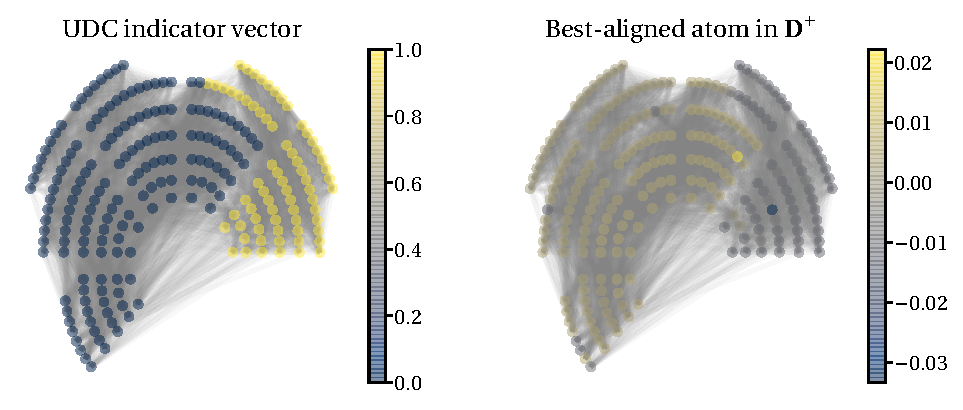
\includegraphics[width=0.9\textwidth]{snc_udc_indicator_and_closest_pinv_atom.pdf}
    \caption[A piecewise-constant signal that is compatible with the graph structure]{A piecewise-constant signal that is compatible with the graph structure. In the Swiss National Council graph depicted above, council members are linked by similarity in their voting patterns. The left image displays the indicator vector of the right-wing UDC party. Its best match among the columns (atoms) of the matrix $\mathbf{D}^+$, in terms of inner product, is shown on the right. Since $\mathbf{D}^+$ depends on the graph alone, the UDC party is fairly well encoded in the edge distribution and forms an effective community in the network.}
    \label{fig:snc_udc_indicator_and_closest_pinv_atom}
\end{figure}

Let us turn our attention now to the $\ell_2$ version of problem \eqref{eq:lp_reg_compact_set}. Unlike before, the measurement matrix $\mathbf{A}$ makes an appearance on the representer theorem.

\begin{theorem}\label{thm:l2_representer}
    Consider problem \eqref{eq:lp_reg_compact_set}, with $p=2$, and use the same set of assumptions as in Theorem \ref{thm:l1_representer}. Then, \emph{all} the points of the solution set $\mathcal{M}_2$ are of the form
    \begin{equation}
        \mathbf{z}^\star = \mathbf{D}^+ \mathbf{A}^\top \mathbf{v} + \mathbf{b}^\star,
    \end{equation}
    where $\mathbf{v} \in \mathbb{R}^{m}$ is a fixed vector, and $\mathbf{b}^\star \in \operatorname{null} \left ( \mathbf{D} \right )$.
\end{theorem}

Both theorems \ref{thm:l1_representer} and \ref{thm:l2_representer} include an unavoidable term in the null space of $\mathbf{D}$, but the solution set induced by the Dirichlet form depends explicitly on the measurement matrix $\mathbf{A}$. Unser \etal \cite{unser2016} use this contrast to argue that $\ell_1$ regularization is better at imposing prior information \emph{despite} the form of the measurements. This position will become even more appealing in Chapter \ref{ch:numerical_tour}, where I show that the recovery error of the Dirichlet form decoder is more sensitive to $\mathbf{A}$ than to the graph connections represented in $\mathbf{D}$.

\section{Relevant recovery results in the literature}

Problems with (potentially) redundant dictionaries~\footnote{The matrix $\mathbf{D}$ in $\|\mathbf{Dx}\|_1$ is often called dictionary or analysis operator because it maps $\mathbf{x}$ to a potentially sparse representation.} such as \eqref{eq:l1_regression} have been studied in \acrlong{cs} at least since Rauhut \etal \cite{rauhut2008} and Cand\`es \etal \cite{candes2011}. If $\mathbf{D}$ were a tight frame and $\mathbf{A}$ a Gaussian matrix, then the recovery error $\|\mathbf{z}^\star - \mathbf{x}\|_2$ of any solution $\mathbf{z}^\star$ to \eqref{eq:l1_regression} would be inversely proportional to $s := \|\mathbf{Dx}\|_0$, with an optimal dependence on the noise level \cite[Theorem 1.2]{candes2011}. The argument that Cand\`es \etal use to show this relies on $\mathbf{A}$ satisfying a certain $\mathbf{D}$-\acrlong{rip}. The number $(N - s)$~\footnote{Recall that $\mathbf{D} \in \mathbb{R}^{N \times n}$.} is sometimes called the cosparsity level of $\mathbf{x}$ under the analysis operator $\mathbf{D}$. Nam \etal \cite{nam2013} and Kabanava and Rauhut \cite{kabanava2015} are good places to find more results about cosparse models in compressed sensing. Still, these papers focus on frames for dictionaries Gaussian matrices measurements. Our graph gradient matrix is not a frame~\footnote{Due to its non-trivial null-space.}, and our measurement vectors are not Gaussian.

In Kabanava \etal~\cite{kabanava2015a} and Krahmer \etal~\cite{krahmer2017} we start to see difference operators being used as the analysis transform, but the measurements are still (sub-)Gaussian-like. Poon \cite{poon2015} also studies \acrlong{tv} minimization but in the context of weighted Fourier sampling. All of these works restrict themselves to signals lying on the Euclidean grid, so their difference matrix $\mathbf{D}$ can be interpreted as the graph gradient of the grid graph. I would like to be able to deal with more general graphs. Kabanava \etal \cite{kabanava2015a} attack the \acrlong{tv} problem by examining the descent cone of $\|\mathbf{D} \cdot\|_1$ and deriving a direct certificate of recovery, a strategy that we will explore in Chapter \ref{ch:lower_bound_min_gain}. Poon \cite{poon2015}, on the other hand, employs a golfing scheme, derived from the properties of the subgradient of $\|\mathbf{D} \cdot\|_1$, arriving at a so-called dual certificate. This is the line of work developed in Chapter \ref{ch:inexact_dual}, which is also greatly informed by the work of Boyer \etal \cite{boyer2019}.

One can also refer to Jung \etal \cite{jung2016, jung2017, jung2018} for a more network-oriented perspective on \acrlong{tv} recovery problems. Under their ``clustering hypothesis'', a piecewise-constant graph signal naturally induces a partition of the vertices into disjoint clusters. The sampled vertices are said to ``resolve'' the partition if they satisfy the \acrlong{nnsp} defined below.

\begin{definition}[\acrfull{nnsp}\protect{\cite{jung2016}}]
    The measurement matrix $\mathbf{A}$ satisfies the \acrshort{nnsp} \acrlong{wrt} an edge set $\mathcal{S} \subseteq \mathcal{E}$ if
    \begin{equation}
        \left \| \glsname{PS} \mathbf{D u} \right \|_1 \leq \frac{1}{2} \left \| (\mathbf{I}_n - \glsname{PS}) \mathbf{D u} \right \|_1,
    \end{equation}
    for any $\mathbf{u} \in \operatorname{null} \left ( \mathbf{A} \right ) \setminus \{ \mathbf{0} \}$.
\end{definition}

Similarly to other null-space properties in compressed sensing, the \acrshort{nnsp} is shown to imply exact recovery in the interpolation problem \eqref{eq:l1_interpolation}.

\begin{proposition}[\protect{\cite{jung2016}}]
    If $\mathbf{A}$ satisfies the \acrshort{nnsp} \acrshort{wrt} $\mathcal{S} = \operatorname{supp}\left ( \mathbf{D x} \right )$, then $\mathbf{x}$ is the unique solution \eqref{eq:l1_interpolation}.
\end{proposition}

Jung \textit{et al.} \cite{jung2016} give deterministic conditions upon which the sampled vertices resolve the partition induced by a piecewise signal of interest. These conditions look into the hop distances of sampled vertices to the borders of the partition, but do not otherwise inform how to design an optimal \emph{random} sampling for the recovery problem.

In this thesis, I approach optimal sampling design for the decoders \eqref{eq:l1_interpolation} and \eqref{eq:l1_regression} in a similar manner as Puy \etal \cite{puy2016} did. They showed that a type of coherence-weighted sampling can minimize the number of rows that $\mathbf{A}$ needs to represent an approximate isometry map for bandlimited graph signals. The decoder is naturally constructed by penalizing non-bandlimited vectors. In our case, we have decoders \eqref{eq:l1_interpolation} and \eqref{eq:l1_regression} that were hand-picked for another class of graph signals, piecewise-constant. But the optimal sampling design is still deduced by minimizing the sample complexity of the decoder with respect to the vertex sampling probabilities $\bm{\pi} = (\pi_i, \dots, \pi_n)$.

What kind of sample complexity expressions can one expect? Readers familiar with \acrlong{cs} might know that $m = \mathcal{O} \left( s \log (n/s) \right)$ random Gaussian measurements are enough to recover, with high probability, any $s$-sparse vector via $\ell_1$ minimization~\cite[Chapter 9]{foucart2013}. The ``sparsity-level'' in \acrfull{gtv} problems is $s := \|\mathbf{Dx}\|_0$, which is the number of edges in the jump-set $\mathcal{S} := \operatorname{supp}\left ( \mathbf{Dx} \right )$ of signal $\mathbf{x}$. Can one hope for sample complexity thresholds in \eqref{eq:l1_interpolation} that are proportional to $\|\mathbf{Dx}\|_0$? Surprisingly, such thresholds appear in the work of Lee \etal~\cite{lee2018}. They even apply for coordinate sampling, and have accompanying optimal designs. Why not just adapt Lee \etal's work to the context of graph signals to answer the main question in this thesis?

The reason is that Lee \etal~\cite{lee2018}'s bounds can be vacuous when dealing with graphs signals. I will show in Chapter \ref{ch:numerical_tour} examples where $|\mathcal{S}|$ is large in comparison to the number of vertices, but we can still successfully interpolate the respective signals using relatively few samples. For such large jump-sets, Lee \etal~\cite{lee2018} would prescribe a number of measurements, $m$, larger than the total number of vertices, $n$. Therefore our sample complexity should be more than just a function of the cardinality of the jump-set and potentially depend on the signal-to-be-recovered~\footnote{Results with this characteristic are often called ``non-uniform'' in \acrlong{cs}. They are named in contrast with results that are valid for a whole class of signals sharing a certain descriptive parameter. For example, any statement containing ``... for all $s$-sparse vectors ...'' is a uniform result.}.

This conclusion is not particularly new in the context of analysis-sparse (or co-sparse) models. Recent studies make a good case for considering only non-uniform guarantees whenever the decoder computes the $\ell_1$ norm in the image of a non-invertible analysis operator $\mathbf{D}$. For instance, Giryes \etal~\cite{giryes2015, giryes2015a} show that no algorithm can accurately recover a co-sparse signal from a number of measurements proportional to the signal's manifold dimension. Meanwhile, Genzel \etal~\cite{genzel2017a} construct two examples of analysis operators for which a signal has the same cosparsity level, but lead to completely different recovery thresholds~\footnote{Genzel \etal~\cite{genzel2017a} prescribe instead thresholds that depend on the partition of the Gram matrix $\mathbf{D} \mathbf{D}^\top$ by the support $\mathcal{S} := \operatorname{supp}\left ( \mathbf{Dx} \right )$. Through $\mathcal{S}$, their guarantee depends on $\mathbf{x}$, hence is non-uniform.}. Once again, those observations are to reinforce the fact that one should avoid naively using sample complexity thresholds proportional to $\|\mathbf{Dx}\|_0$ in problems like \eqref{eq:f_interpolation}.


\section{Summary and final notes}

The variational principle is a popular paradigm for recovering signals from subsampled linear measurements. Among all vectors satisfying the observation constraints, the returned solution is the one that minimizes a loss function $f$. This function is often chosen to be convex for analytical and numerical reasons.

There is also precedent in the literature for setting the search space directly, without resorting to a penalty $f$. Problems of the type ``$\underset{z \in \mathbb{R}^{n}}{\min} \| \mathbf{Az - y} \|_q^q \text{ subject to } \mathbf{z} \in \mathcal{K}$'', where $\mathcal{K}$ is a convex set, are sometimes called the $\mathcal{K}$-lasso \cite{plan2016}. Despite the difference at first sight, there is a $\rho > 0$ for which the $\mathcal{K}$-lasso becomes equivalent to \eqref{eq:f_regression} by setting $\mathcal{K} = \{\mathbf{z} \in \mathbb{R}^{n}: f(\mathbf{z}) \leq \rho \}$~\footnote{This can be proved by the method of Lagrange multipliers \cite[Chapter 5]{boyd2009}.}. Some researchers, like Bora \etal~\cite{bora2017a}, might even use non-convex constraint sets $\mathcal{K}$. They set out to recover images of human faces from few pixel measurements, having access to a pre-trained Generative Adversarial Network (GAN). This GAN excels in creating natural-looking faces, so Bora \etal argue that its range can be used as the recovery search space. It is an implicit way to avoid points in $\mathbb{R}^{n}$ that do not look like human faces, but it definitely makes the problem harder to study mathematically.

The \acrshort{gtv} semi-norm is a good penalty choice for recovering piecewise-constant signals on graphs. These signals have a sparse representation in terms of the extreme points of the \acrshort{gtv} ball. As a result, $\mathcal{D}(\| \mathbf{D} \cdot \|_1, \mathbf{x})$ should be fairly narrow when $\mathbf{x}$ is piecewise constant, making it easier for a trivial intersection with $\operatorname{null} \left ( \mathbf{A} \right )$ to take place. Ultimately, the trivial intersection is what guarantees the exact recovery of $\mathbf{x}$ from $\mathbf{Ax}$. I have also argued that minimizing $\|\mathbf{D} \cdot\|_1$ is preferable to minimizing $\|\mathbf{D} \cdot\|_2^2$ if we want solutions less dependent on the form of the measurement matrix.

Our main decoders, \eqref{eq:l1_interpolation} and \eqref{eq:l1_regression}, fall under the scope of co-sparse models in \acrlong{cs}. But the most relevant work in this field (Lee \etal~\cite{lee2018}) prescribes sample complexity bounds that are potentially vacuous when dealing with graph signals. In the end, I have to reach new recovery guarantees from scratch, with the next two chapters compiling attempts to do so. Chapter \ref{ch:lower_bound_min_gain} deals with a gain functional certifying that the descent cone $\mathcal{D}(\| \mathbf{D} \cdot \|_1, \mathbf{x})$ and the subspace $\operatorname{null} \left ( \mathbf{A} \right )$ intersect only at $\mathbf{0}$. In parallel, Chapter \ref{ch:inexact_dual} uses the characteristics of the subdifferential $\partial \| \mathbf{D} \cdot \|_1(\mathbf{x})$ as a blueprint to iteratively build a recovery certificate.

\clearpage

\begin{subappendices}
    \section{Geometry of the \texorpdfstring{\acrshort{gtv}}{G-TV} semi-norm}

    \subsection{Proof of Proposition \ref{prop:character_l1_analysis_descent_cone}}\label{sec:proof_character_l1_analysis_descent_cone}
    Here I adapt \cite[Lemma 4.1]{krahmer2019}, where Krahmer and St\"{o}ger characterize the descent cone of the matrix spectral norm. But first, let me precise the notion of polarity for cones.

\begin{definition}[Polar cone]\label{def:polar_cone}
    Let $\mathcal{K} \subset \mathbb{R}^{n}$ be a cone. The corresponding polar cone, denoted $\mathcal{K}^{\mathsf{o}}$, is the set
    \begin{equation}
        \mathcal{K}^{\mathsf{o}} := \{ \mathbf{v} \in \mathbb{R}^{n} : \langle \mathbf{v}, \mathbf{u} \rangle \leq 0, \forall \mathbf{u} \in \mathcal{K}\}.
    \end{equation}
\end{definition}

I will say that a vector $\mathbf{v}$ is polar to a set $\mathcal{S}$ if $\langle \mathbf{v}, \mathbf{s}\rangle \leq 0, \forall \mathbf{s} \in \mathcal{S}$. Similarly, $\mathbf{v}$ is polar to another vector $\mathbf{u}$ if $\langle \mathbf{v}, \mathbf{u}\rangle \leq 0$.

\begin{proof}
    \pf\ The desired expressions are a consequence of the subdifferential $\partial \|\mathbf{D} \cdot\|_1(\mathbf{x})$ being polar to $\mean{\mathcal{D}(\| \mathbf{D} \cdot \|_1, \mathbf{x})}$ \cite[Thm. 23.7]{rockafellar1970}. Recall from Proposition \ref{prop:character_subdifferential_l1} that $\mathbf{v} \in \partial \|\mathbf{D} \cdot\|_1(\mathbf{x})$ if and only if $\mathbf{v} = \mathbf{D}^\top \operatorname{sign} \left ( \mathbf{Dx} \right ) + \mathbf{D}^\top (\mathbf{I}_N - \mathbf{P}_{\mathcal{S}}) \mathbf{w}$, for some $\mathbf{w} \in \mathbb{R}^{N}$ satisfying $\left\|(\mathbf{I}_N - \mathbf{P}_{\mathcal{S}}) \mathbf{w}\right\|_\infty \leq 1$. We then split the argument in two parts:

    \step{}{
        ``$\impliedby$'': If $\left\langle \operatorname{sign} \left ( \mathbf{Dx} \right ), \mathbf{Du} \right\rangle \leq -\left\|(\mathbf{I}_N - \mathbf{P}_{\mathcal{S}}) \mathbf{Du}\right\|_1$ then $\mathbf{u} \in \mean{\mathcal{D}(\| \mathbf{D} \cdot \|_1, \mathbf{x})}$.
    }
        \begin{proof}
            \pf\ For any given $\mathbf{v} \in \mean{\mathcal{D}(\| \mathbf{D} \cdot \|_1, \mathbf{x})}\polar$, directly compute
            \begin{align*}
                \langle \mathbf{v}, \mathbf{u} \rangle & = \left\langle \mathbf{D}^\top \operatorname{sign} \left( \mathbf{Dx} \right) + \mathbf{D}^\top (\mathbf{I}_N - \mathbf{P}_{\mathcal{S}}) \mathbf{w}, \mathbf{u} \right\rangle \\
                & = \left\langle \operatorname{sign} \left ( \mathbf{Dx} \right ), \mathbf{Du} \right\rangle + \left\langle (\mathbf{I}_N - \mathbf{P}_{\mathcal{S}}) \mathbf{w}, \mathbf{Du} \right \rangle \\
                & \leq \left\langle \operatorname{sign} \left ( \mathbf{Dx} \right ), \mathbf{Du} \right\rangle + \left\|(\mathbf{I}_N - \mathbf{P}_{\mathcal{S}}) \mathbf{Du}\right\|_1 \cdot \underbrace{\left\|(\mathbf{I}_N - \mathbf{P}_{\mathcal{S}}) \mathbf{w}\right\|_\infty}_{\leq 1} & \comment{H\"older inequality} \\
                & \leq 0. & \comment{Assumption}
            \end{align*}
            Therefore, $\mathbf{u}$ is polar to $\mean{\mathcal{D}(\| \mathbf{D} \cdot \|_1, \mathbf{x})}\polar$, meaning $\mathbf{u} \in \mean{\mathcal{D}(\| \mathbf{D} \cdot \|_1, \mathbf{x})}$.\hfill\qedsymbol
        \end{proof}

    \step{}{
        ``$\implies$'': If $\mathbf{u} \in \mean{\mathcal{D}(\| \mathbf{D} \cdot \|_1, \mathbf{x})}$ then $\left\langle \operatorname{sign} \left ( \mathbf{Dx} \right ), \mathbf{Du} \right\rangle \leq -\left\|(\mathbf{I}_N - \mathbf{P}_{\mathcal{S}}) \mathbf{Du}\right\|_1$.
    }
        \begin{proof}
            \pf\
            \step{}{
                Pick a vector $\mathbf{w} \in \mathbb{B}_{\infty}^N$ for which $\langle \mathbf{w}, (\mathbf{I}_N - \mathbf{P}_{\mathcal{S}}) \mathbf{Du}\rangle = \left\|(\mathbf{I}_N - \mathbf{P}_{\mathcal{S}}) \mathbf{Du}\right\|_1$. Then $\mathbf{v} = \mathbf{D}^\top \operatorname{sign} \left ( \mathbf{Dx} \right ) + \mathbf{D}^\top (\mathbf{I}_N - \mathbf{P}_{\mathcal{S}}) \mathbf{w}$ is a valid subgradient in $\partial \|\mathbf{D} \cdot\|_1(\mathbf{x})$, because
                \begin{equation*}
                    \left\|(\mathbf{I}_N - \mathbf{P}_{\mathcal{S}}) \mathbf{w}\right\|_\infty \leq \underbrace{\left\|(\mathbf{I}_N - \mathbf{P}_{\mathcal{S}})\right\|_\infty}_{\leq 1} \cdot \underbrace{\left\|\mathbf{w}\right\|_\infty}_{\leq 1} \leq 1.
                \end{equation*}
            }
            \step{}{
                Since $\mathbf{v} \in \partial \|\mathbf{D} \cdot\|_1(\mathbf{x})$ is polar to $\mean{\mathcal{D}(\| \mathbf{D} \cdot \|_1, \mathbf{x})}$, we conclude that
                \begin{align*}
                    0 & \geq \langle \mathbf{u}, \mathbf{v} \rangle & \comment{Assumption} \\
                    & = \left\langle \mathbf{D}^\top \operatorname{sign} \left( \mathbf{Dx} \right) + \mathbf{D}^\top (\mathbf{I}_N - \mathbf{P}_{\mathcal{S}}) \mathbf{w}, \mathbf{u} \right\rangle \\
                    & = \left\langle \operatorname{sign} \left ( \mathbf{Dx} \right ), \mathbf{Du} \right\rangle + \left\|(\mathbf{I}_N - \mathbf{P}_{\mathcal{S}}) \mathbf{Du}\right\|_1. & \comment{Choice of $\mathbf{w}$}
                \end{align*}
            }
            \qedsymbol
        \end{proof}
    \qedstep
\end{proof}

    \subsection{Proof of Proposition \ref{prop:extreme_points_gtv_ball}}\label{sec:proof_extreme_gtv}
    I will need to establish some notation before delving into the argument.

\begin{definition}[Graph cut]
    The \emph{graph cut} associated with two vertex sets $\mathcal{S}_1, \mathcal{S}_2 \subset [n]$ is the set
    \begin{equation}
        \operatorname{cut}\left(\mathcal{S}_1, \mathcal{S}_2\right) := \left\{ e = \left(v_i, v_j\right) \in \mathcal{E} : (i \in \mathcal{S}_1 \wedge j \in \mathcal{S}_2) \vee (j \in \mathcal{S}_1 \wedge i \in \mathcal{S}_2)\right\}.
    \end{equation}
    We also define the size of $\operatorname{cut}\left(\mathcal{S}_1, \mathcal{S}_2\right)$ to be
    \begin{equation}
        \left|\operatorname{cut}\left(\mathcal{S}_1, \mathcal{S}_2\right)\right| := \sum_{i \in \mathcal{S}_1} \sum_{j \in \mathcal{S}_2} \sqrt{W_{ij}}.
    \end{equation}
\end{definition}

\begin{definition}[Up-to-additive-constant extreme point]
    We say that $\mathbf{t} \in \mathcal{S}$ is an up-to-additive-constant extreme point of $\mathcal{S}$ when we can write $\mathbf{t} = \beta \mathbf{s} + (1 - \beta) \mathbf{u}$, using $\beta \in (0,1)$ and $\mathbf{s}, \mathbf{u} \in \mathcal{S}$, only if $\mathbf{s} - \mathbf{t} = c_s \mathbf{1}$ and $\mathbf{u} - \mathbf{t} = c_u \mathbf{1}$, for some constants $c_s, c_u \in \mathbb{R}$.
\end{definition}

Lastly, define also the following \emph{level sets} of $\mathbf{t} \in \mathbb{R}^{n}$, indexed by $v \in \mathbb{R}$:
\begin{align}
    \mathcal{S}_{v}(\mathbf{t}) := \{i \in \mathbb{R}: t_i = v\} \\
    \mathcal{S}_{v^{+}}(\mathbf{t}) := \{i \in \mathbb{R}: t_i > v\} \\
    \mathcal{S}_{v^{-}}(\mathbf{t}) := \{i \in \mathbb{R}: t_i < v\}.
    \end{align}

I will prove a slightly stronger claim than the one stated in the main text: the up-to-additive-constants extreme points $\mathbf{t}^\star$ of \glsname{Bgtv} are of the form
\begin{equation}
    \mathbf{t}^\star = |\operatorname{cut}(\mathcal{S}_{v_1}(\mathbf{t}^\star), \mathcal{S}_{v_2}(\mathbf{t}^\star))| \cdot \mathbb{1}_{\mathcal{S}_{v_2}(\mathbf{t}^\star)} + v_1 \mathbf{1}.
\end{equation}
The argument is adapted from Szlam \etal~\cite{szlam2010}.

\begin{proof}
    \pf\  Let $v_1 < v_2 < \dots < v_d \in \mathbb{R}$ be all the distinct values taken by the coordinates of some $\mathbf{t} \in \mathbb{R}^{n}$. Trivially, $1 \leq d \leq n$. I will split the argument into the cases $d = 1$, $d = 2$, and $d \geq 3$, and show that $\mathbf{t}$ is an extreme point of \glsname{Bgtv} if and only if $d = 2$. The precise expression for $\mathbf{t}^\star$ will appear as a consequence of the computations in the proof.

    \step{}{If $d = 1$, $\mathbf{t}$ is not an extreme point of \glsname{Bgtv}.}
        \begin{proof}
            \pf\ Vector $\mathbf{t} = v_1 \mathbf{1}$ is constant, so $\|\mathbf{Dt}\|_1 = \sum_{(i,j)} \sqrt{W_{i,j}} |v_1 - v_1| = 0$. Since $\|\mathbf{Dt}\|_1 < 1$, vector $\mathbf{t}$ cannot be an extreme point of \glsname{Bgtv}.
        \end{proof}

    \step{}{If $d \geq 3$ and $\|\mathbf{Dt}\|_1 = 1$, $\mathbf{t}$ is still not an extreme point of \glsname{Bgtv}.}
        \begin{proof}
            \pf\ I will construct perturbations $\mathbf{s} := \mathbf{t} + \varepsilon_p \mathbb{1}_{\mathcal{S}_{v_p}(\mathbf{t})} - \varepsilon_q \mathbb{1}_{\mathcal{S}_{v_q}(\mathbf{t})}$ and $\mathbf{u} := \mathbf{t} - \varepsilon_p \mathbb{1}_{\mathcal{S}_{v_p}(\mathbf{t})} + \varepsilon_q \mathbb{1}_{\mathcal{S}_{v_q}(\mathbf{t})}$, for some small $\varepsilon_p, \varepsilon_q > 0$ and some $v_p, v_q \in \{v_1, \dots, v_d\}$. With these constructions, I show that $\mathbf{s}, \mathbf{u} \in \glsname{Bgtv}$. Since $\mathbf{t} = \frac{1}{2}\mathbf{s} + \frac{1}{2}\mathbf{u}$, this will imply that $\mathbf{t}$ cannot be an extreme point of \glsname{Bgtv}.
            \step{}{
                Note first that if we pick any positive $\varepsilon < \underset{k \neq l \in [d]}{\min} \enspace |v_k - v_l|$ the effect of the perturbation $\varepsilon \mathbb{1}_{\mathcal{S}_{v}(\mathbf{t})}$ decouples from $\| \mathbf{Dt} \|_1$:
                \begin{align*}
                    \| \mathbf{D} (\mathbf{t} + \varepsilon \mathbb{1}_{\mathcal{S}_{v}(\mathbf{t})}) \|_1 & = \sum_{(i,j) \in \mathcal{E}} \sqrt{W_{ij}} \left |t_i - t_j + \varepsilon \mathbb{1}_{\mathcal{S}_{v}(\mathbf{t})}(i) - \varepsilon \mathbb{1}_{\mathcal{S}_{v}(\mathbf{t})}(j) \right | \\
                    & = 2 \sum_{i \in \mathcal{S}_{v^{-}(\mathbf{t})}}\sum_{j \in \mathcal{S}_{v}(\mathbf{t})} \sqrt{W_{ij}} \underbrace{|t_i - t_j - \varepsilon|}_{= t_j - t_i + \varepsilon} \\
                    & \quad + 2 \sum_{i \in \mathcal{S}_{v}(\mathbf{t})}\sum_{j \in \mathcal{S}_{v}(\mathbf{t})} \sqrt{W_{ij}} |t_i - t_j| \\
                    & \quad + 2\sum_{i \in \mathcal{S}_{v}(\mathbf{t})}\sum_{j \in \mathcal{S}_{v^{+}}(\mathbf{t})} \sqrt{W_{ij}} \underbrace{|t_i - t_j + \varepsilon|}_{= t_j - t_i - \varepsilon} \\
                    & = \| \mathbf{Dt} \|_1 + \varepsilon \left ( \underbrace{\left [ \sum_{i \in \mathcal{S}_{v^{-}}(\mathbf{t})}\sum_{j \in \mathcal{S}_{v}(\mathbf{t})} \sqrt{W_{ij}} \right ]}_{=: \left|\operatorname{cut}\left(\mathcal{S}_{v^{-}}(\mathbf{t}), \mathcal{S}_{v}(\mathbf{t})\right)\right|} - \underbrace{\left [ \sum_{i \in \mathcal{S}_{v}(\mathbf{t})}\sum_{j \in \mathcal{S}_{v^{+}}(\mathbf{t})} \sqrt{W_{ij}} \right ]}_{=: \left|\operatorname{cut}\left(\mathcal{S}_{v^{+}}(\mathbf{t}), \mathcal{S}_{v}(\mathbf{t})\right)\right|} \right ). \\
                \end{align*}
            }
            \step{}{
                Therefore, if we pick $\varepsilon_p, \varepsilon_q < \frac{1}{2} \underset{k \neq l \in [d]}{\min} \enspace |v_k - v_l|$, we can write the \acrshort{gtv} semi-norm of $\mathbf{s}$ as
                \begin{align*}
                    \| \mathbf{Ds} \|_1 & = \left \| \mathbf{D} \left (\mathbf{t} + \varepsilon_p \mathbb{1}_{\mathcal{S}_{v_p}(\mathbf{t})} - \varepsilon_q \mathbb{1}_{\mathcal{S}_{v_q}(\mathbf{t})} \right ) \right \|_1 \\
                    & = \underbrace{\| \mathbf{Dt} \|_1}_{=1} + \varepsilon_p \left ( \left|\operatorname{cut}(\mathcal{S}_{v_p^{-}(\mathbf{t})}, \mathcal{S}_{v_p}(\mathbf{t})) \right| - \left|\operatorname{cut}(\mathcal{S}_{v_p^{+}(\mathbf{t})}, \mathcal{S}_{v_p}(\mathbf{t}))\right| \right ) \\
                    & \qquad\qquad\ - \varepsilon_q \left ( \left|\operatorname{cut}(\mathcal{S}_{v_q^{-}(\mathbf{t})}, \mathcal{S}_{v_q}(\mathbf{t}))\right| - \left|\operatorname{cut}(\mathcal{S}_{v_q^{+}(\mathbf{t})}, \mathcal{S}_{v_q}(\mathbf{t}))\right| \right ) \\
                \end{align*}
                and, similarly for $\mathbf{u}$,
                \begin{align*}
                    \| \mathbf{Du} \|_1 & = \left\| \mathbf{D} \left(\mathbf{t} - \varepsilon_p \mathbb{1}_{\mathcal{S}_{v_p}(\mathbf{t})} + \varepsilon_q \mathbb{1}_{\mathcal{S}_{v_q}(\mathbf{t})}\right)\right\|_1 \\
                    & = 1 - \varepsilon_p \left ( \left|\operatorname{cut}(\mathcal{S}_{v_p^{-}(\mathbf{t})}, \mathcal{S}_{v_p}(\mathbf{t}))\right| - \left|\operatorname{cut}(\mathcal{S}_{v_p^{+}(\mathbf{t})}, \mathcal{S}_{v_p}(\mathbf{t}))\right| \right ) \\
                    & \qquad + \varepsilon_q \left ( \left|\operatorname{cut}(\mathcal{S}_{v_q^{-}(\mathbf{t})}, \mathcal{S}_{v_q}(\mathbf{t}))\right| - \left|\operatorname{cut}(\mathcal{S}_{v_q^{+}(\mathbf{t})}, \mathcal{S}_{v_q}(\mathbf{t}))\right| \right ) \\
                \end{align*}
            }
            \step{}{
                For both $\mathbf{s}$ and $\mathbf{u}$ to be on $\operatorname{bd}(\glsname{Bgtv})$, \textit{i.e.}, $\| \mathbf{Ds} \|_1 = \| \mathbf{Du} \|_1 = 1$, it suffices to pick $\varepsilon_p, \varepsilon_q$ such that
                \begin{equation*}
                    \varepsilon_p = \varepsilon_q \left ( \frac{\left|\operatorname{cut}\left(\mathcal{S}_{v_q^{-}(\mathbf{t})}, \mathcal{S}_{v_q}(\mathbf{t})\right)\right| - \left|\operatorname{cut}\left(\mathcal{S}_{v_q^{+}(\mathbf{t})}, \mathcal{S}_{v_q}(\mathbf{t})\right)\right|}{\left|\operatorname{cut}\left(\mathcal{S}_{v_p^{-}(\mathbf{t})}, \mathcal{S}_{v_p}(\mathbf{t})\right)\right| - \left|\operatorname{cut}\left(\mathcal{S}_{v_p^{+}(\mathbf{t})}, \mathcal{S}_{v_p}(\mathbf{t})\right)\right|} \right ).
                \end{equation*}
            }
            \step{}{
                We conclude that $\mathbf{t}$ is not an extreme point of \glsname{Bgtv}, because $\mathbf{t} = \frac{1}{2}\mathbf{s} + \frac{1}{2}\mathbf{u}$ and $\mathbf{s}, \mathbf{u} \in \glsname{Bgtv}$.
            }
        \end{proof}

    \step{}{If $d = 2$ and $\|\mathbf{Dt}\|_1 = 1$, $\mathbf{t}$ is an (up-to-additive-constant) extreme point of \glsname{Bgtv}.}
        \begin{proof}
            \pf\ It suffices to show that if $\mathbf{t} = \beta \mathbf{s} + (1 - \beta) \mathbf{u}$ for some $\beta \in (0,1)$ and $\mathbf{s} ,\mathbf{u} \in \operatorname{bd}(\glsname{Bgtv})$ with $\mathbf{s} \neq \mathbf{u}$, then $\mathbf{s}$ and $\mathbf{u}$ differ from $\mathbf{t}$ only by a constant.
            \step{}{
                Since $\mathbf{t} = (v_2 - v_1) \mathbb{1}_{\mathcal{S}_{v_2}}  + v_1 \mathbf{1}$, $\mathbf{Dt}$ is supported on the edges in $\operatorname{cut} (\mathcal{S}_{v_2}\left(\mathbf{t}), \mathcal{S}_{v_1}(\mathbf{t})\right) \subset \mathcal{E}$.
            }
            \step{}{
                Define a new graph $\mathcal{R} = (\mathcal{V}, \mathcal{E}|_{\operatorname{cut} (\mathcal{S}_{v_2}\left(\mathbf{t}), \mathcal{S}_{v_1}(\mathbf{t})\right)})$ which is the restricted version of the original graph $\mathcal{G}$ to the edges in $\operatorname{cut} (\mathcal{S}_{v_2}\left(\mathbf{t}), \mathcal{S}_{v_1}(\mathbf{t})\right)$. Correspondingly, define a new graph difference operator $\mathbf{D}_{\mathcal{R}}$ by setting to zero the entries in $\mathbf{D}$ related to the edges in the complement of $\operatorname{cut} (\mathcal{S}_{v_2}\left(\mathbf{t}), \mathcal{S}_{v_1}(\mathbf{t})\right)$.
            }
            \step{}{
                By construction, the graph \acrshort{tv} semi-norm of $\mathbf{t}$ is conserved in this new graph, \textit{i.e.}, $\|\mathbf{Dt}\|_1 = \|\mathbf{D}_{\mathcal{R}} \mathbf{t}\|_1 = 1$.
            }
            \step{}{
                I can then use the triangle inequality to get the relation
                \begin{align*}
                    1 & = \|\mathbf{D}_{\mathcal{R}} \mathbf{t}\|_1 \\
                    & = \|\mathbf{D}_{\mathcal{R}} (\beta \mathbf{s} + (1 - \beta) \mathbf{u}) \|_1 \\
                    & \leq \beta \|\mathbf{D}_{\mathcal{R}} \mathbf{s}\|_1 + (1 - \beta) \|\mathbf{D}_{\mathcal{R}} \mathbf{v}\|_1.
                \end{align*}
            }
            \step{}{
                On the other hand, $\| \mathbf{Dt} \|_1 := \sum_{(i,j)} \sqrt{W_{ij}} |t_i - t_j|$ is monotonically decreasing \acrshort{wrt} the edge weights, and $\mathcal{R}$ had fewer edges than $\mathcal{G}$. Therefore, since both $\mathbf{s}$ and $\mathbf{u}$ are assumed to be on $\operatorname{bd}(\glsname{Bgtv})$, we thus verify
                \begin{align*}
                    \beta \|\mathbf{D}_{\mathcal{R}} \mathbf{s}\|_1 + (1 - \beta) \|\mathbf{D}_{\mathcal{R}} \mathbf{v}\|_1 & \leq \beta \underbrace{\|\mathbf{D} \mathbf{s}\|_1}_{=1} + (1 - \beta) \underbrace{\|\mathbf{D} \mathbf{v}\|_1}_{=1} \\
                    & = \beta + (1 - \beta) \\
                    & = 1.
                \end{align*}
            }
            \step{}{
                By the two previous steps, we must have $\|\mathbf{D} \mathbf{s}\|_1 = \|\mathbf{D}_{\mathcal{R}} \mathbf{s}\|_1 = \|\mathbf{D}_{\mathcal{R}} \mathbf{u}\|_1 = \|\mathbf{D} \mathbf{u}\|_1 = 1$. Hence, both $\mathbf{Ds}$ and $\mathbf{Du}$ must also be supported on $\operatorname{cut} (\mathcal{S}_{v_2}\left(\mathbf{t}), \mathcal{S}_{v_1}(\mathbf{t})\right)$.
            }
            \step{}{
                Finally, having verified that $\mathbf{Dt},\mathbf{Ds}, \mathbf{Du}$ share the same support, and that $\|\mathbf{D} \mathbf{t}\|_1 = \|\mathbf{D} \mathbf{s}\|_1 = \|\mathbf{D} \mathbf{u}\|_1$, we must conclude that $\mathbf{t,s,u}$ can differ only by elements on the null space of $\mathbf{D}$. The latter corresponds to the space of vectors of the form $c \mathbf{1}$, for $c \in \mathbb{R}$, so the claim is proved.~\qedsymbol
            }
        \end{proof}

    \step{}{If $d = 2$ and $\mathbf{t}^\star$ is an (up-to-additive-constants) extreme point of \glsname{Bgtv}, then $\mathbf{t}^\star = |\operatorname{cut}(\mathcal{S}_{v_1}(\mathbf{t}^\star), \mathcal{S}_{v_2}(\mathbf{t}^\star))| \cdot \mathbb{1}_{\mathcal{S}_{v_2}(\mathbf{t}^\star)} + v_1 \mathbf{1}$.}
        \begin{proof}
            \pf\ This is just a computation exercise. Since $\mathbf{t}^\star = (v_2 - v_1) \mathbb{1}_{\mathcal{S}_{v_2}} + v_1 \mathbf{1}$ and $\|\mathbf{Dt}^\star\|_1 = 1$, we obtain the identity
            \begin{align*}
                1 & = \|\mathbf{Dt}^\star\|_1 \\
                & = \sum_{(i,j)} \sqrt{W_{ij}} |t_i - t_j| \\
                & = 2 \sum_{i \in \mathcal{S}_{v_2}}\sum_{j \in \mathcal{S}_{v_1}} \sqrt{W_{ij}} (v_2 - v_1) \\
                & = 2 \left|\operatorname{cut} (\mathcal{S}_{v_2}\left(\mathbf{t}^\star), \mathcal{S}_{v_1}(\mathbf{t}^\star)\right)\right| \cdot (v_2 - v_1).
            \end{align*}
            Therefore, $(v_2 - v_1) = \frac{1}{2 \left|\operatorname{cut} (\mathcal{S}_{v_2}\left(\mathbf{t}^\star), \mathcal{S}_{v_1}(\mathbf{t}^\star)\right)\right|}$.~\qedsymbol
        \end{proof}

    \qedstep{We have exhausted the options for the number $d$ of distinct coordinates, so $\mathbf{t}$ is an extreme point of \glsname{Bgtv} if and only if $d = 2$. Furthermore, any such extreme point is of the form $2|\operatorname{cut}(\mathcal{S}_{v_1}(\mathbf{t}^\star), \mathcal{S}_{v_2}(\mathbf{t}^\star))| \cdot \mathbb{1}_{\mathcal{S}_{v_2}(\mathbf{t}^\star)} + v_1 \mathbf{1}$.}
\end{proof}

    \section{Representer theorems}\label{sec:proof_representer}
    Throughout this appendix, we will consider problems of the type
\begin{equation}
    \mathcal{M}_p = \underset{\mathbf{z} \in \mathbb{R}^{n}}{\min} \| \mathbf{D z} \|_p^p \text{ such that } \mathbf{Az} \in \mathcal{C} \tag{\ref{eq:lp_reg_compact_set}},
\end{equation}
with $p \geq 1$, and assume that
\begin{align}
    \tag{A1} \label{ass:representer_null} \operatorname{null} \left ( \mathbf{D} \right ) \cap \operatorname{null} \left ( \mathbf{A} \right ) = \{ \mathbf{0} \}\\
    \tag{A2} \label{ass:representer_compact_convex} \mathcal{C} \subset \mathbb{R}^{m} \text{ is compact and convex} \\
    \tag{A3} \label{ass:representer_feasible} \mathbf{A}^{-1}(\mathcal{C}) := \{\mathbf{z} \in \mathbb{R}^{n}: \mathbf{Az} \in \mathcal{C}\} \text{ is non-empty}.
\end{align}
The representer theorems I will prove are based on the work of Unser~\etal~\cite{unser2016}, but here I extend their results to operators $\mathbf{D}$ without a right-inverse.~\footnote{A matrix has a right inverse if and only if it represents a surjective linear map. Our graph gradient operator, $\mathbf{D} \in \mathbb{R}^{N \times n}$, is not guaranteed to have a right inverse because $N > n$ in general --- hence $\mathbf{D}$ cannot represent a surjective map.} The first basic fact that I need to establish is the following characterization of the sets $\mathcal{M}_p$, for $p \geq 1$. It follows the reasoning of Unser~\etal~\cite[Lemma 20]{unser2016}.

\begin{lemma}\label{lem:nonempty-convex-compact}
    For any $p \geq 1$, $\mathcal{M}_p$ is a non-empty, convex, and compact subset of $\mathbb{R}^{n}$.
\end{lemma}

The proof relies on features of the interactions between linear maps and convex, compact sets, as well as on properties of norms in finite-dimensional spaces. I begin by characterizing the pre-image $\mathbf{A}^{-1}(\mathcal{C})$. Then, I use the Bolzano-Weierstrass theorem to show that $\mathcal{M}_p$ is not empty. Finally, writing $\mathcal{M}_p$ as an intersection of ``well-behaved'' sets, we can conclude that it must be convex and compact.

\begin{proof}

    \pf\

    \step{pf:closed}{
        $\mathbf{A}^{-1}(\mathcal{C})$ is closed because $\mathcal{C}$ is closed and the linear map $L: \mathbf{z} \mapsto \mathbf{Az}$ is continuous.
    }
    \step{pf:convex}{
        $\mathbf{A}^{-1}(\mathcal{C})$ is also convex, because the pre-image of a convex set $\mathcal{C}$ by a linear map is convex.
    }
    \step{}{
        $\mathcal{M}_p$ is non-empty.
    }
        \begin{proof}
            \pf\
            \step{}{
                For notation sake, let $\gamma := \underset{\mathbf{z} \in \mathbf{A}^{-1}(\mathcal{C})}{\inf} \| \mathbf{Dz}\|_p^p$
            }
            \step{}{
                Let $(\mathbf{z}^{(i)})_{i \in \mathbb{N}}$ be a sequence of elements of $\mathbf{A}^{-1}(\mathcal{C})$ inducing a \emph{decreasing} sequence $(\| \mathbf{Dz}^{(i)}\|_p^p)_{i \in \mathbb{N}}$ of norms such that $\underset{i \to \infty}{\lim \, \inf} \| \mathbf{Dz}^{(i)}\|_p^p = \gamma$.
            }
            \step{}{
                For each $i \in \mathbb{N}$, decompose $\mathbf{z}^{(i)}$ uniquely as $\mathbf{z}^{(i)} = \mathbf{D}^+ \mathbf{a}^{(i)} + \mathbf{b}^{(i)}$, where $\mathbf{a}^{(i)} = \mathbf{Dz}^{(i)}$ is an element of $\operatorname{range} \left( \mathbf{D}^\top \right)$ and $\mathbf{b}^{(i)}$ is an element of $\operatorname{null} \left ( \mathbf{D} \right )$.
            }
            \step{}{
                The sequence $(\mathbf{a}^{(i)})_{i \in \mathbb{N}}$ is bounded, because $\|\mathbf{a}^{(i)}\|_p^p = \| \mathbf{Dz}^{(i)}\|_p^p \leq \| \mathbf{Dz}_{i-1}\|_p^p \leq \dots \leq \| \mathbf{Dz}_1 \|_p^p$.
            }
            \step{}{
                The sequence $(\mathbf{b}^{(i)})_{i \in \mathbb{N}}$ is also bounded.
            }
                \begin{proof} \pf\
                    To see this, note that assumption \ref{ass:representer_null}implies $\| \mathbf{b}^{(i)} \|_p^p \leq c \|\mathbf{Ab}^{(i)}\|_p^p$ for some positive constant $c > 0$. Then, compute
                    \begin{align*}
                        \| \mathbf{b}^{(i)} \|_p^p & \leq c \|\mathbf{Ab}^{(i)}\|_p^p \\
                        & = c \|\mathbf{Az}^{(i)} - \mathbf{AD^+a}^{(i)}\|_p^p \\
                        & \leq c \| \mathbf{Az}^{(i)} \|_2 + c \|\mathbf{AD^+a}^{(i)}\|_p^p.
                    \end{align*}
                    The left term on the \acrshort{rhs}, $\| \mathbf{Az}^{(i)} \|_p^p$, is bounded because $\mathbf{Az}^{(i)} \in \mathcal{C}$ and $\mathcal{C}$ is a compact set. The right term is bounded  because $\mathbf{a}^{(i)}$ is bounded and $\mathbf{AD}^+$ is a finite dimensional linear operator, hence bounded. \qedsymbol
                \end{proof}
            \step{}{
                We can then extract a sub-sequence from $(\mathbf{z}^{(i)})_{i \in \mathbb{N}}$ that converges to some point $\mathbf{z}^{(\infty)} = \mathbf{D}^+ \mathbf{a}^{(\infty)} + \mathbf{b}^{(\infty)}$.
            }
                \begin{proof} \pf\
                    Bolzano-Weierstrass theorem, using the boundedness of both $(\mathbf{a}^{(i)})_{i \in \mathbb{N}}$ and $(\mathbf{b}^{(i)})_{i \in \mathbb{N}}$ sequences. \qedsymbol
                \end{proof}
            \step{}{
                The converging point $\mathbf{z}^{(\infty)}$ must satisfy $\| \mathbf{Dz}^{(\infty)}\|_p^p \leq \gamma$.
            }
                \begin{proof}
                    \pf\ Indeed, $\| \mathbf{Dz}^{(\infty)}\|_p^p \leq \| \mathbf{Dz}^{(i)}\|_p^p$, for any $i \in \mathbb{N}$, due to the sequence \\ $(\| \mathbf{Dz}^{(i)}\|_p^p)_{i \in \mathbb{N}}$ being decreasing. Therefore, taking the limit on both sides of this inequality, $\mathbf{z}^{(\infty)}$ must satisfy $\| \mathbf{Dz}^{(\infty)}\|_p^p \leq \underset{\mathbf{z} \in \mathbf{A}^{-1}(\mathcal{C})}{\inf} \| \mathbf{Dz}\|_p^p =: \gamma$. \qedsymbol
                \end{proof}
            \step{}{
                On the other hand, $\| \mathbf{Dz}^{(\infty)}\|_p^p \geq \underset{\mathbf{z} \in \mathbf{A}^{-1}(\mathcal{C})}{\inf} \| \mathbf{Dz}\|_p^p =: \gamma$ because $\mathbf{A}^{-1}(\mathcal{C})$ is closed, containing all limits of sequences of its elements.
            }
            \step{}{
                $\| \mathbf{Dz}^{(\infty)}\|_p^p = \gamma$, so $\mathcal{M}_p$ contains at least one point, namely $\mathbf{z}^{(\infty)}$.
            }
            \qedsymbol
        \end{proof}

        \step{}{
            Finally, I can show that $\mathcal{M}_p$ is both convex and compact.
        }
            \begin{proof}
                \pf\
                \step{}{
                    Let $\mathcal{L}_p = \left \{\mathbf{z} \in \mathbb{R}^{n} : \| \mathbf{Dz}\|_p^p \leq \gamma \right \}$. We can write $\mathcal{M}_p$ as the intersection $\mathcal{M}_p = \mathcal{L}_p \cap \mathbf{A}^{-1}(\mathcal{C}) = \left \{ \left [ \mathcal{L}_p \cap \operatorname{range} \left( \mathbf{D} \right) \right ] \cap \mathbf{A}^{-1}(\mathcal{C}) \right \} \oplus \left \{ \left [ \mathcal{L} \cap \operatorname{null} \left( \mathbf{D} \right) \right ] \cap \mathbf{A}^{-1}(\mathcal{C}) \right\}$.
                }
                \step{}{
                    $\mathcal{L}_p \cap \operatorname{range} \left( \mathbf{D} \right)$ is convex and compact because it is a norm ball in a subset of $\mathbb{R}^{n}$.
                }
                \step{}{
                    Hence, $\left [ \mathcal{L}_p \cap \operatorname{range} \left( \mathbf{D} \right) \right ] \cap \mathbf{A}^{-1}(\mathcal{C})$ is both convex and compact, by virtue of being the intersection of two convex sets, one closed and the other compact.
                }
                \step{}{
                    For the second term in the direct sum, consider splitting the feasible set as $\mathbf{A}^{-1}(\mathcal{C}) = \left [ \mathbf{A}^{-1}(\mathcal{C}) \cap \operatorname{range} \left( \mathbf{A}^\top \right) \right ] \oplus \left [ \mathbf{A}^{-1}(\mathcal{C}) \cap \operatorname{null} \left ( \mathbf{A} \right ) \right ]$. The first term is a one-to-one linear mapping from $\mathcal{C}$ to a set in $\mathbb{R}^{n}$. Therefore, the compactness of $\mathcal{C}$ implies the compactness of $\left [ \mathbf{A}^{-1}(\mathcal{C}) \cap \operatorname{range} \left( \mathbf{A}^\top \right) \right ]$. Moreover, the latter is a hyperplane slice of a convex set, so it is itself convex. As for the term $\left [ \mathbf{A}^{-1}(\mathcal{C}) \cap \operatorname{null} \left ( \mathbf{A} \right ) \right ]$, it is the empty set if $\mathbf{0} \notin \mathcal{C}$, or equal to $\operatorname{null} \left ( \mathbf{A} \right )$ otherwise.
                }
                \step{}{
                    Since $\|\mathbf{Dz}\|_p^p = 0 \iff \mathbf{z} \in \operatorname{null} \left ( \mathbf{D} \right )$, we have the identity $\mathcal{L}_p \cap \operatorname{null} \left( \mathbf{D} \right) = \operatorname{null} \left ( \mathbf{D} \right )$. Thus, by assumption \ref{ass:representer_null},
                    \begin{equation*}
                        \left [ \mathcal{L}_p \cap \operatorname{null} \left( \mathbf{D} \right) \right ] \cap \left [ \mathbf{A}^{-1}(\mathcal{C}) \cap \operatorname{null} \left ( \mathbf{A} \right ) \right ] = \left \{
                        \begin{matrix}
                            \emptyset & \text{if } \mathbf{0} \notin \mathcal{C} \\
                            \{ \mathbf{0} \} & \text{otherwise}.
                        \end{matrix}
                        \right.
                    \end{equation*}
                    In any case,
                    \begin{align*}
                        \left [ \mathcal{L}_p \cap \operatorname{null} \left( \mathbf{D} \right) \right ] \cap \mathbf{A}^{-1}(\mathcal{C}) & = \operatorname{null} \left( \mathbf{D} \right) \cap \left \{ \left [ \mathbf{A}^{-1}(\mathcal{C}) \cap \operatorname{range} \left( \mathbf{A}^\top \right) \right ] \oplus \left [ \mathbf{A}^{-1}(\mathcal{C}) \cap \operatorname{null} \left ( \mathbf{A} \right ) \right ] \right \}\\
                        & = \operatorname{null} \left( \mathbf{D} \right) \cap \left [ \mathbf{A}^{-1}(\mathcal{C}) \cap \operatorname{range} \left( \mathbf{A}^\top \right) \right ],
                    \end{align*}
                    which is a hyperplane slice of a convex and compact set, thus also convex and compact.
                }
                \step{}{
                    At last, we conclude that $\mathcal{M}_p$ is both convex and compact, because those properties are preserved under direct sum.
                }
                \qedsymbol
            \end{proof}
        \qedstep
\end{proof}


\subsection{Proof of Theorem \ref{thm:l1_representer}}\label{ap:representer_l1}

Let me restate below an informal reminder of this section's goal.

\begin{claim}
    The extreme points $\mathbf{z}^\star$ of $\mathcal{M}_1$ are of the form $\mathbf{z}^\star = \mathbf{D}^+ \mathbf{a}^\star + \mathbf{b}^\star$, where $\mathbf{a}^\star$ has at most $m$ non-zero coordinates, and $\mathbf{b}^\star \in \operatorname{null} \left ( \mathbf{D} \right )$.
\end{claim}

The main tool we will need is the next lemma.

\begin{lemma}\label{lem:l1_sparse_extreme}
    Let $\mathbf{D}(\mathbf{A}^{-1}(\mathcal{C})) := \{ \mathbf{Dz} \in \mathbb{R}^{N} : \mathbf{Az} \in \mathcal{C} \subset \mathbb{R}^{m} \}$. The extreme points of the set
    \begin{equation}
        \widetilde{\mathcal{M}_1} := \underset{\mathbf{a} \in \mathbf{D}(\mathbf{A}^{-1}(\mathcal{C}))}{\min} \| \mathbf{a} \|_1
    \end{equation}
    have at most $m$ non-zero coefficients.
\end{lemma}

The proof can be deduced from \cite[Theorem 6]{unser2016}, but I give the full argument here for completeness.

\begin{proof}
    \pf\
    \step{}{
        First of all, $\widetilde{\mathcal{M}_1}$ is non-empty, convex and compact. This is a consequence of Lemma \ref{lem:nonempty-convex-compact}, with the linear transformation $\mathbf{z} \mapsto \mathbf{Dz}$ mapping $\mathcal{M}_1$ to $\widetilde{\mathcal{M}_1}$.
    }
    \step{}{
        By the Krein-Milman theorem, $\widetilde{\mathcal{M}_1}$ is then the closed convex hull of its extreme points.
    }
    \step{}{
        Let $\mathbf{a}^\star$ be one such extreme point, chosen arbitrarily. I will show that $\| \mathbf{a}^\star \|_0 \leq m$, implying the main claim.
    }
        \begin{proof} \pf\
        \step{}{
            For notation sake, let $\gamma := \underset{\mathbf{a} \in \mathbf{D}(\mathbf{A}^{-1}(\mathcal{C}))}{\min} \| \mathbf{a} \|_1$, so that $\|\mathbf{a}^\star\|_1 = \gamma$.
        }
        \step{}{
            Prooceed by contradiction, assuming that $\| \mathbf{a}^\star \|_0 \geq m + 1$. Without loss of generality, we can say that $\{\mathbf{a}^{\star}_j\}_{j = 1}^{m+1}$ forms a set of non-zero coordinates of $\mathbf{a}^\star$.
        }
        \step{}{
            Define a new vector $\mean{\mathbf{a}} := \mathbf{a}^\star - \sum_{j=1}^{m+1} \mathbf{a}^{\star}_j \mathbf{e}_j$, where $\{\mathbf{e}_j\}_{j=1}^N$ forms the standard basis in $\mathbb{R}^{N}$. Note that by construction $\mean{\mathbf{a}}$ and $\mathbf{a}^\star$ have disjoint supports.
        }
        \step{}{
            Now, for each $j \in [m+1]$, define $\mathbf{v}_j := \mathbf{AD}^+(\mathbf{a}^{\star}_j \mathbf{e}_j) \in \mathbb{R}^{m}$. Since any collection of $m+1$ vectors in $\mathbb{R}^{m}$ is linearly dependent, there must exist constants $c_1, c_2, \dots, c_{m+1}$ for which $\sum_{j=1}^{m+1} c_j \mathbf{v}_j = \mathbf{0}$.
        }
        \step{}{
            Using these same constants, define a new vector in $\mathbb{R}^{N}$ through $\mathbf{a}_0 := \sum_{j=1}^{m+1} c_j \mathbf{a}^{\star}_j \mathbf{e}_j$. We already know that $\mathbf{a}^\star \in \mathbf{D}(\mathbf{A}^{-1}(\mathcal{C}))$, but we further remark that the perturbations $\mathbf{a}^\star - \varepsilon \mathbf{a}_0$ and $\mathbf{a}^\star + \varepsilon \mathbf{a}_0$ are also both in $\mathbf{D}(\mathbf{A}^{-1}(\mathcal{C}))$, for any $\varepsilon > 0$.
        }
            \begin{proof}
                \pf\ $\mathbf{A D}^+ \mathbf{a}_0 = \sum_{j=1}^{m+1} c_j \mathbf{v}_j = \mathbf{0}$ by construction. Hence, $\mathbf{A D}^+ (\mathbf{a}^\star - \varepsilon \mathbf{a}_0) = \mathbf{A D}^+ \mathbf{a}^\star = \mathbf{A D}^+ (\mathbf{a}^\star + \varepsilon \mathbf{a}_0)$ for any $\varepsilon > 0$. \qedsymbol
            \end{proof}
        \step{}{
            I now claim that $\sum_{j=1}^{m+1} c_j |\mathbf{a}^{\star}_j| = 0$, implying $\|\mathbf{a}^\star \pm \varepsilon \mathbf{a}_0\|_1 = \gamma$.
        }
            \begin{proof} \pf\
                \step{}{
                    Suppose otherwise that $\sum_{j=1}^{m+1} c_j |\mathbf{a}^{\star}_j| \neq 0$, and pick $\varepsilon \in \left (\frac{-1}{\underset{j \in [m+1]}{\max} |c_j|}, \frac{1}{\underset{j \in [m+1]}{\max} |c_j|} \right )$. Then either $\|(\mathbf{a}^\star - \varepsilon \mathbf{a}_0)\|_1 < \gamma$ or $\|(\mathbf{a}^\star + \varepsilon \mathbf{a}_0)\|_1 < \gamma$.
                }
                    \begin{proof} \pf\
                        This follows by computing
                        \begin{align*}
                            \|(\mathbf{a}^\star \pm \varepsilon \mathbf{a}_0)\|_1 & = \left \| \mean{\mathbf{a}} + \sum_{j=1}^{m+1} (1 \pm \varepsilon c_j) \mathbf{a}^{\star}_j \mathbf{e}_j \right \|_1 \\
                            & \underset{\text{disjoint support}}{=} \|\mean{\mathbf{a}}\|_1 + \sum_{j=1}^{m+1} |1 \pm \varepsilon c_j| |\mathbf{a}^{\star}_j|\\
                            & \underset{\text{choice of } \varepsilon}{=} \|\mean{\mathbf{a}}\|_1 + \sum_{j=1}^{m+1} (1 \pm \varepsilon c_j) |\mathbf{a}^{\star}_j|\\
                            & \underset{\text{reordering}}{=} \|\mathbf{a}\|_1 \pm \sum_{j=1}^{m+1} \varepsilon c_j |\mathbf{a}^{\star}_j|\\
                            & = \gamma \pm \sum_{j=1}^{m+1} \varepsilon c_j |\mathbf{a}^{\star}_j|.~\qedsymbol
                        \end{align*}
                    \end{proof}
                \step{}{
                    But since $\gamma = \underset{\mathbf{a} \in \mathbf{D}(\mathbf{A}^{-1}(\mathcal{C}))}{\min} \| \mathbf{a} \|_1$ and we have established that both $\mathbf{a}^\star \pm \varepsilon \mathbf{a}_0$ belong to $\mathbf{D}(\mathbf{A}^{-1}(\mathcal{C}))$, the conclusion of the last step is absurd. Thus, \\ $\sum_{j=1}^{m+1} c_j |\mathbf{a}^{\star}_j| = 0$ and $\|\mathbf{a}^\star \pm \varepsilon \mathbf{a}_0\|_1 = \gamma$, as claimed.
                }
                \qedsymbol
            \end{proof}
        \step{}{
            A direct consequence of $\|\mathbf{a}^\star \pm \varepsilon \mathbf{a}_0\|_1 = \gamma$ is then that $\mathbf{a}^\star \pm \varepsilon \mathbf{a}_0 \in \widetilde{\mathcal{M}_1}$
        }
        \step{}{
            We have reached our contradiction: we are able to write $\mathbf{a}^\star$ as the convex combination $\mathbf{a}^\star = \frac{1}{2}(\mathbf{a}^\star + \varepsilon \mathbf{a}_0) + \frac{1}{2}(\mathbf{a}^\star - \varepsilon \mathbf{a}_0)$ of two points in $\widetilde{\mathcal{M}_1}$. Thus, $\mathbf{a}^\star$ \emph{cannot} be an extreme point of $\widetilde{\mathcal{M}_1}$.
        }
        \qedsymbol
        \end{proof}
    \qedstep
        \begin{proof}
            Any extreme point of $\widetilde{\mathcal{M}_1} \subset \mathbb{R}^{N}$ must have at most $m$ non-zero coordinates.
        \end{proof}
\end{proof}

With Lemma \ref{lem:l1_sparse_extreme} at hand, I am finally ready to prove Theorem \ref{thm:l1_representer}.

\begin{proof}

    \textsc{Proof of Theorem \ref{thm:l1_representer}:}\
    \step{}{
        The extreme points $\mathbf{z}^\star$ of $\mathcal{M}_1$ satisfy the equation $\mathbf{D z}^\star = \mathbf{a}^\star$, where $\mathbf{a}^\star$ has at most $m$ non-zero coefficients.
    }
        \begin{proof} \pf\
            Applying the change of variable $\mathbf{D z} = \mathbf{a}$, call on Lemma \ref{lem:l1_sparse_extreme} and realize that the extreme points of $\mathcal{M}_1$ are mapped to the extreme points of $\widetilde{\mathcal{M}_1}$ through the linear transformation $\mathbf{z} \mapsto \mathbf{Dz}$.~\qedsymbol
        \end{proof}
    \step{}{
        We can express any $\mathbf{z} \in \mathbb{R}^{n}$ as $\mathbf{z} = \mathbf{D}^+ \mathbf{D} \mathbf{z} + (\mathbf{I}_n - \mathbf{D}^+ \mathbf{D})\mathbf{z}$, by seeing $\mathbb{R}^{n}$ as a direct sum between $\operatorname{range} \left( \mathbf{D}^\top \right)$ and $\operatorname{null} \left ( \mathbf{D} \right )$.
    }
    \qedstep
        \begin{proof}
            Any extreme point of $\mathbf{z}^\star$ of $\mathcal{M}_1$ takes the form $\mathbf{z}^\star = \mathbf{D}^+ \mathbf{D} \mathbf{z}^\star + \mathbf{b}^\star = \mathbf{D}^+ \mathbf{a}^\star + \mathbf{b}^\star$, for some $\mathbf{b}^\star \in \operatorname{null} \left ( \mathbf{D} \right )$, and $\mathbf{a}^\star \in \mathbb{R}^{N}$ satisfying $\|\mathbf{a}^\star \|_0 \leq m$.
        \end{proof}
\end{proof}


\subsection{Proof of Theorem \ref{thm:l2_representer}}\label{ap:representer_l2}

This section's goal is the following:

\begin{claim}
    All the points in $\mathcal{M}_2$ are of the form $\mathbf{z}^\star = \mathbf{D}^+ \mathbf{DA}^\top \mathbf{v} + \mathbf{b}^\star$, where $\mathbf{v} \in \mathbb{R}^{m}$ is a fixed vector, and $\mathbf{b}^\star \in \operatorname{null} \left ( \mathbf{D} \right )$.
\end{claim}

This time I adapt \cite[Theorems 5, 9, 18]{unser2016} to use as our main tool.

\begin{lemma}\label{lem:l2_unique_solution}
    Let $\mathbf{D}(\mathbf{A}^{-1}(\mathcal{C})) := \{ \mathbf{Dz} \in \mathbb{R}^{N} : \mathbf{Az} \in \mathcal{C} \subset \mathbb{R}^{m} \}$. The set
    \begin{equation}
        \widetilde{\mathcal{M}_2} := \underset{\mathbf{a} \in \mathbf{D}(\mathbf{A}^{-1}(\mathcal{C}))}{\min} \| \mathbf{a} \|_2^2
    \end{equation}
    has a single point, $\mathbf{a}^\star$. Furthermore, this point is of the form $\mathbf{a}^\star = \mathbf{Dr}^\star$ for some $\mathbf{r} \in \operatorname{range} \left( \mathbf{A}^\top \right)$.
\end{lemma}

\begin{proof}
    \pf\
    \step{}{
        The set $\mathbf{D}(\mathbf{A}^{-1}(\mathcal{C}))$ is convex and closed because it is a linear mapping of a convex and closed set $\mathcal{C}$. It is also non-empty because $\mathbf{A}^{-1}(\mathcal{C})$ is assumed to be non-empty.
    }
    \step{}{
        The solution set $\widetilde{\mathcal{M}_2}$ contains thus a single point, namely the the orthogonal projection of the origin, $\mathbf{0}$, onto the convex set $\mathbf{D}(\mathbf{A}^{-1}(\mathcal{C}))$. Let us call this single point $\mathbf{a}^\star$.
    }
    \step{}{
        Let $\mathbf{z}^\star$ be a point in $\mathbb{R}^{n}$ such that $\mathbf{a}^\star = \mathbf{D z}^\star$. Decompose this point as $\mathbf{z}^\star = \mathbf{r}^\star + \mathbf{n}^\star$, where $\mathbf{r}^\star \in \operatorname{range} \left( \mathbf{A}^\top \right)$ and $\mathbf{n}^\star \in \operatorname{null} \left ( \mathbf{A} \right )$. Then, we must have $\mathbf{n}^\star = \mathbf{0}$.
    }
        \begin{proof}
            \pf\
            \step{}{
                By assumption \ref{ass:representer_null}, the orthogonal projection operators $\mathbf{D^+D}$ and $\mathbf{A^+A}$ commute.
            }
            \step{}{
                This commutative property leads to the fact $\| \mathbf{Dz}^\star \|_2^2 = \| \mathbf{Dr}^\star \|_2^2 + \| \mathbf{Dn}^\star \|_2^2$. Indeed,
                \begin{align*}
                    \| \mathbf{Dz}^\star \|_2^2 & = \| \mathbf{Dr}^\star \|_2^2 + 2 \langle \mathbf{Dn}^\star, \mathbf{Dr}^\star \rangle +  \| \mathbf{Dn}^\star \|_2^2 \\
                    & = \| \mathbf{Dr}^\star \|_2^2 + 2 \langle \mathbf{n}^\star, \mathbf{D^\top Dr}^\star \rangle + \| \mathbf{Dn}^\star \|_2^2 \\
                    & \underset{\text{for some } \mathbf{z} \in \mathbb{R}^{n}}{=} \| \mathbf{Dr}^\star \|_2^2 + 2 \langle \mathbf{n}^\star, \mathbf{D^+ D A^+ A z}^\star \rangle + \| \mathbf{Dn}^\star \|_2^2 \\
                    & \underset{\text{commutativity}}{=} \| \mathbf{Dr}^\star \|_2^2 + 2 \langle \underbrace{\mathbf{n}^\star}_{\in \operatorname{null} \left ( \mathbf{A} \right )}, \underbrace{\mathbf{A^+ A D^+ D z}^\star}_{\in \operatorname{range} \left( \mathbf{A^\top} \right)} \rangle + \| \mathbf{Dn}^\star \|_2^2 \\
                    & = \| \mathbf{Dr}^\star \|_2^2 + 0 + \| \mathbf{Dn}^\star \|_2^2 \\
                \end{align*}
            }
            \step{}{
                The term $\mathbf{n}^\star$ must be in $\operatorname{null} \left ( \mathbf{D} \right )$.
            }
                \begin{proof} \pf\
                    To see this, note that $\mathbf{A z}^\star = \mathbf{A r}^\star$, so $\mathbf{A r}^\star$ is also in $\mathbf{D}(\mathbf{A}^{-1}(\mathcal{C}))$. But because $\mathbf{D z}^\star$ is a norm minimizer, together with the result from the previous step, that $\|\mathbf{D r}^\star\|_2^2 \geq \|\mathbf{D z}^\star\|_2^2 = \| \mathbf{Dr}^\star \|_2^2 + \| \mathbf{Dn}^\star \|_2^2 \iff \| \mathbf{Dn}^\star \|_2^2 = 0$. Hence, $\mathbf{n}^\star \in \operatorname{null} \left ( \mathbf{D} \right )$.~\qedsymbol
                \end{proof}
            \step{}{
                In summary, $\mathbf{n}^\star \in \operatorname{null} \left ( \mathbf{A} \right ) \cap \operatorname{null} \left ( \mathbf{D} \right )$. Calling upon assumption \ref{ass:representer_null} once again, we conclude that $\mathbf{n}^\star = \mathbf{0}$.
            }
            \qedsymbol
        \end{proof}
    \qedstep
        \begin{proof}
            The single point belonging to $\widetilde{\mathcal{M}_2}$ has the form $\mathbf{a}^\star = \mathbf{Dr}^\star$, for some $\mathbf{r}^\star \in \operatorname{range} \left( \mathbf{A}^\top \right)$.
        \end{proof}
\end{proof}

Finally, proving Theorem \ref{thm:l2_representer} is very similar to proving Theorem \ref{thm:l1_representer}, but this time I call on Lemma \ref{lem:l2_unique_solution} instead of Lemma \ref{lem:l1_sparse_extreme}.

\begin{proof}

    \textsc{Proof of Theorem \ref{thm:l2_representer}:}\
    \step{}{
        Every point $\mathbf{z}^\star \in \mathcal{M}_2$ satisfies the equation $\mathbf{D z}^\star = \mathbf{DA}^\top \mathbf{v}$, for a fixed vector $\mathbf{v} \in \mathbb{R}^{m}$.
    }
        \begin{proof} \pf\
            With the change of variable $\mathbf{D z} = \mathbf{a}$, apply Lemma \ref{lem:l2_unique_solution} and realize that the points of $\mathcal{M}_2$ are all mapped to the single point in $\widetilde{\mathcal{M}_2}$ through the linear transformation $\mathbf{z} \mapsto \mathbf{Dz}$.~\qed
        \end{proof}
    \step{}{
        We can express any $\mathbf{z} \in \mathbb{R}^{n}$ as $\mathbf{z} = \mathbf{D}^+ \mathbf{D} \mathbf{z} + (\mathbf{I}_n - \mathbf{D}^+ \mathbf{D})\mathbf{z}$.
    }
    \qedstep
        \begin{proof}
            Any point of $\mathbf{z}^\star$ of $\mathcal{M}_2 \subset \mathbb{R}^{n}$ takes the form $\mathbf{z}^\star = \mathbf{D}^+ \mathbf{D} \mathbf{z}^\star + \mathbf{b}^\star = \mathbf{D}^+ \mathbf{DA}^\top \mathbf{v} + \mathbf{b}^\star$, for a fixed vector $\mathbf{v} \in \mathbb{R}^{m}$, and some $\mathbf{b}^\star \in \operatorname{null} \left ( \mathbf{D} \right )$.
        \end{proof}
\end{proof}
\end{subappendices}
\chapter{Direct certificates: measurement gain inside the descent cone}
\label{ch:lower_bound_min_gain}

In Chapter \ref{ch:recovery_convex} I hinted at how the geometry of the descent cone influences the correctness of the solutions to the \emph{interpolation} problem \eqref{eq:f_interpolation}. In this chapter, I will show which sense of narrowness in the descent cones can lead to robust recovery guarantees for \emph{regression} problems \eqref{eq:f_regression}, and in particular \eqref{eq:l1_regression}. Recall that the regression setting admits noisy measurements of the type $\mathbf{y} = \mathbf{Ax} + \mathbf{e}$ where we have a bound, $\|\mathbf{e}\|_q^q \leq \eta$, on the noise level.

Notions of width appear as a consequence of translating the trivial intersection property from Theorem~\ref{thm:trivial_intersection_suffices} into something computable. This quantity is a positive lower bound on the measurement operator's gain restricted to the descent cone. I this lower bound a direct recovery certificate, in contrast to the dual certificates investigated in the next chapter.

Strategies for lower bounding the minimum gain vary according to which random matrix plays the role of measurement operator. It is enlightening at first to imagine what would happen if we had Gaussian measurement vectors. Then, I introduce Mendelson's small-ball method as a potential path towards a direct certificate in our setting. Unfortunately, the ``spikiness'' of our coordinate-sampling matrices proves to be a burden down this road.

The chapter finishes with an open question, but points towards a way to get a direct certificate for robust recovery in \eqref{eq:l1_regression}. A way that requires knowing more about the \emph{coordinate structure} of descent cones induced by the \acrshort{gtv} semi-norm. Ultimately, the sample complexity of \acrshort{gtv} decoders only gets a workable expression in Chapter \ref{ch:inexact_dual}.


\section{A positive gain functional as a recovery certificate}

We can quantify the the trivial intersection property in terms of any $q$-norm by noting that
\begin{equation}
    \mathcal{D}(f, \mathbf{x}) \cap \operatorname{null} \left ( \mathbf{A} \right ) = \{ \mathbf{0} \} \iff \|\mathbf{Au}\|_q^q > 0, \forall \mathbf{u} \in \mathcal{D}(f, \mathbf{x}) \setminus \{ \mathbf{0} \}.
    \label{eq:trivial_intersect_equiv_lower_bound_gain}
\end{equation}
This motivates the definition of a minimum gain functional as a computable proxy for the property.

\begin{definition}[Minimum $q$-gain]\label{def:min_q_gain}
    For any $q \geq 1$, the minimum $q$-gain of a measurement operator $\mathbf{A}$, restricted to the descent cone $\mathcal{D}( f, \mathbf{x})$ is the quantity
    \begin{equation}
        \gamma_{\min}^{(q)} \left ( \mathcal{D}( f, \mathbf{x}), \mathbf{A} \right ) = \underset{\mathbf{u} \in \mathcal{D}(f, \mathbf{x}) \cap \operatorname{bd}(\mathbb{B}^{n}_q)}{\inf} \enspace \|\mathbf{A u}\|_q^q.
    \end{equation}
\end{definition}

The \acrlong{rhs} of \eqref{eq:trivial_intersect_equiv_lower_bound_gain} now simply reads as $ \gamma_{\min}^{(q)} \left ( \mathcal{D}( f, \mathbf{x}), \mathbf{A} \right ) > 0$. Automatically, by Theorem~\ref{thm:trivial_intersection_suffices}, we conclude that a positive minimum $q$-gain yields the uniqueness of $\mathbf{x}$ as a solution of the \emph{interpolation} problem \eqref{eq:f_interpolation}. In the literature, $\sqrt{\gamma_{\min}^{(2)} \left ( \mathcal{D}( f, \mathbf{x}), \mathbf{A} \right )}$ is also known as simply ``minimum gain''~\cite{chandrasekaran2012}, or ``minimum conic singular value''~\cite{tropp2015a}. Rather than being a mere numeric translation of a geometric property, minimum gain functionals also inform on the robustness of convex recovery programs to noise.

A \emph{regression} program of the type
\begin{equation*}
    \underset{\mathbf{z} \in \mathbb{R}^{n}}{\min} f(\mathbf{Dz}) \text{ subject to } \| \mathbf{Az - y} \|_q^q \leq \eta. \tag{P$f$-$\eta$}
\end{equation*}
recovers $\mathbf{x}$ robustly from $\mathbf{y} = \mathbf{Ax} + \mathbf{e}$ if any solution $\mathbf{z}^\star$ is as close to $\mathbf{x}$ as the noise $\mathbf{e}$ permits. Theorem \ref{thm:error_min_q_gain} shows how the distance between $\mathbf{z}^\star$ and $\mathbf{x}$ is inversely proportional to the minimum gain functional, and directly proportional to the noise level.

\begin{theorem}[\protect{\cite[Prop. 2.2]{chandrasekaran2012}, \cite[Prop. 2.6]{tropp2015a}, \cite[~Thm. 4]{kabanava2015a}}]\label{thm:error_min_q_gain}
    If $\gamma_{\min}^{(q)} \left ( \mathcal{D}( f, \mathbf{x}), \mathbf{A} \right ) > 0$ and $\|\mathbf{e}\|_q^q \leq \eta$, then any solution $\mathbf{z}^\star$ of problem \eqref{eq:f_regression} satisfies
    \begin{equation}
        \| \mathbf{z}^\star - \mathbf{x}\|_q^q \leq \frac{2 \eta}{\gamma_{\min}^{(q)} \left ( \mathcal{D}( f, \mathbf{x}), \mathbf{A} \right )}.
    \end{equation}
\end{theorem}

Therefore, the larger $\gamma_{\min}^{(q)} \left ( \mathcal{D}( f, \mathbf{x}), \mathbf{A} \right )$, the more robust the corresponding decoder is. Theorem \ref{thm:error_min_q_gain} is a powerful result with a simple proof.

\clearpage

\begin{proof}
    \pf\ A straightforward adaptation of the argument in \cite[~Theorem 4]{kabanava2015a}, connecting two separate inequalities to reach the claim. Let $\mathbf{z}^\star$ be some solution \eqref{eq:f_regression}.
    \step{}{
        $\| \mathbf{z}^\star - \mathbf{x}\|_q^q \leq \frac{\| \mathbf{A} (\mathbf{z}^\star - \mathbf{x})\|_q^q}{\gamma_{\min}^{(q)} \left ( \mathcal{D}( f, \mathbf{x}), \mathbf{A} \right )}$
    }
        \begin{proof}
            \pf
            \step{}{$f(\mathbf{\mathbf{z}^\star}) \leq f(\mathbf{\mathbf{x}})$, because $\mathbf{z}^\star$ is a solution of \eqref{eq:f_regression}.}
            \step{}{Hence, $\mathbf{z}^\star - \mathbf{x} \in \mathcal{D}( f, \mathbf{x})$.}
            \step{}{With $\mathbf{u} := \frac{1}{\| \mathbf{z}^\star - \mathbf{x}\|_q^q} \in \mathcal{D}(f, \mathbf{x}) \cap \mathbb{B}^{n}_q$, we conclude that $\gamma_{\min}^{(q)} \left ( \mathcal{D}( f, \mathbf{x}), \mathbf{A} \right ) \cdot \|\mathbf{u}\|_q^q \leq \|\mathbf{Au}\|_q^q$, by definition of the minimum $q$-gain.}~\qedsymbol
        \end{proof}
    \step{}{
        $\| \mathbf{A} (\mathbf{z}^\star - \mathbf{x})\|_q^q \leq 2 \eta$.
    }
        \begin{proof}
            \pf\ Just use the triangle inequality and the feasibility of both $\mathbf{z}^\star$ and $\mathbf{x}$:
            \begin{align*}
                \| \mathbf{A} (\mathbf{z}^\star - \mathbf{x})\|_q^q & = \| (\mathbf{Az}^\star - \mathbf{y}) - (\mathbf{Ax} - \mathbf{y})\|_q^q \\
                & \leq \| \mathbf{Az}^\star - \mathbf{y} \|_q^q + \| \mathbf{Ax} - \mathbf{y}\|_q^q \\
                & \leq \eta + \eta.
            \end{align*}
            \qedsymbol
        \end{proof}
    \qedstep{$\| \mathbf{z}^\star - \mathbf{x}\|_q^q \leq \frac{\| \mathbf{A} (\mathbf{z}^\star - \mathbf{x})\|_q^q}{\gamma_{\min}^{(q)} \left ( \mathcal{D}( f, \mathbf{x}), \mathbf{A} \right )} \leq \frac{2 \eta}{\gamma_{\min}^{(q)} \left ( \mathcal{D}( f, \mathbf{x}), \mathbf{A} \right )}.$}
\end{proof}

The dependence of $\|\mathbf{z}^\star - \mathbf{x}\|_q^q$ on the noise level is optimal, because all we know about $\mathbf{e}$ is the bound $\|\mathbf{e}\|_q^{q} \leq \eta$. Furthermore, Theorem~\ref{thm:trivial_intersection_suffices} from Chapter~\ref{ch:recovery_convex} becomes a mere corollary, reached by making $\eta \to 0$ in the recovery error bound. Hence there is no loss in considering only regression --- and not interpolation --- problems in this chapter.

In \acrlong{cs}, a metric condition more commonly used than $\gamma_{\min}^{(q)} \left ( \mathcal{D}( f, \mathbf{x}), \mathbf{A} \right ) > 0$ is the \acrfull{rip}, demanding that
\begin{equation}
    c \|\mathbf{z}\|_q \leq \|\mathbf{Az}\|_q \leq C\|\mathbf{z}\|_q, \enspace 0< c < C, \enspace \forall \mathbf{z} \in \mathcal{D}( f, \mathbf{x}).
    \label{eq:rip}
\end{equation}
But \acrlong{lhs} of \eqref{eq:rip} is equivalent to a positive minimum $q$-gain. The \acrshort{rip} is thus a stronger condition; too strong, in fact. Recent research~\cite{dirksen2018a} suggests that the \acrlong{rhs} of \eqref{eq:rip} gives rise to a \emph{gap} between the optimal and the \acrshort{rip}-certifiable numbers of measurements required in $\ell_1$-recovery problems. The reason for the gap seems to be that the inequality $\|\mathbf{Az}\|_q \leq C\|\mathbf{z}\|_q$ requires of $\mathbf{A}$ either very good concentration properties or a large number of rows~\cite{lecue2017}. Despite the popularity of the \acrshort{rip}, I will therefore focus only on how our measurement matrices can be made to satisfy $\gamma_{\min}^{(q)} \left ( \mathcal{D}( f, \mathbf{x}), \mathbf{A} \right ) > 0$.


\section{Interlude: what is known for Gaussian measurements?}

The properties of Gaussian random vectors are among the easiest to characterize theoretically. It is no surprise then that most of the work in convex recovery \cite{chandrasekaran2012, tropp2015a, vershynin2015a, plan2016, liaw2017, plan2017, vershynin2017} (in general), and \acrlong{cs} \cite{foucart2013, foygel2014, dirksen2018, dirksen2018a} (in particular) employ Gaussian measurement ensembles.

Gordon's ``escape through a mesh'' theorem \cite[Cor. 1.2]{gordon1988} connects the minimum $2$-gain of  a Gaussian matrix~\footnote{By ``Gaussian matrix'' I always mean a random matrix whose entries are independent draws from the standard Gaussian distribution.} $\mathbf{A}$ to its number of rows (measurements) through the Gaussian width of the descent cone~\cite[Cor. 3.3]{chandrasekaran2012}. This is notion of conic width through the lens of Gaussian vectors can be defined as follows.

\begin{definition}[Conic Gaussian width \protect{\cite[Def. 3.1]{tropp2015a}}]
    Let $\mathcal{K} \subset \mathbb{R}^{n}$ be a cone and $\mathbf{g} \sim \mathcal{N}(\mathbf{0}, \mathbf{I}_n)$ be a standard Gaussian vector. The conic Gaussian width of $\mathcal{K}$ is the quantity
    \begin{equation}
        w(\mathcal{K}) := \mathbb{E} \left ( \underset{\mathbf{u} \in \mathcal{K} \cap \mathbb{S}^{n-1}}{\sup} \langle \mathbf{g}, \mathbf{u}\rangle \right ).
    \end{equation}
\end{definition}

The conic Gaussian width is computed for the descent cones of some atomic norms in Chandrasekaran \etal~\cite{chandrasekaran2012}. The authors can then use those widths to arrive at the number of Gaussian measurements required for robust recovery in the respective decoders.

More than that, it is even possible to precisely describe the phase transition undergone by the probability of recovery in convex recovery problems with Gaussian measurements. Such a result, derived from conic integral geometry tools, is presented next.

\begin{theorem}[Phase transition \protect{\cite[Thm. II]{amelunxen2014}}]
    \label{thm:phase_transition_gaussian}
    Let $\mathbf{A} \in \mathbb{R}^{m \times n}$ be a random measurement matrix with \acrshort{iid} standard Gaussian entries. Define \texttt{Success} as the event that $\gamma_{\min}^{(q)} \left ( \mathcal{D}( f, \mathbf{x}), \mathbf{A} \right ) > 0$ takes place. Then, for any $\varepsilon \in (0, 1)$
    \begin{equation}
        \left \{
        \begin{matrix}
        m \leq w(\mathcal{D}(f, \mathbf{x}))^2 - \sqrt{8 n \log (4 / \varepsilon)} & \implies & \mathbb{P} \left ( \texttt{Success} \right ) \leq \varepsilon \\
        m \geq w(\mathcal{D}(f, \mathbf{x}))^2 + \sqrt{8 n \log (4/\varepsilon)} + 1 & \implies & \mathbb{P} \left ( \texttt{Success} \right ) \geq 1 - \varepsilon \\
        \end{matrix}
        \right.
    \end{equation}
\end{theorem}

In words, the theorem says that if the number of Gaussian measurements crosses a barrier of $\mathcal{O} \left( \sqrt{n} \right)$, centered at $w(\mathcal{D}(f, \mathbf{x}))^2$, then the probability of success suddenly jumps from almost zero to almost one. Sharp transition phenomena like this one are ubiquitous in high-dimensional geometry \cite{donoho2009a,oymak2018}. Below, I give a brief sketch of the proof of Theorem~\ref{thm:phase_transition_gaussian}, because it complements the geometric intuition from Chapter~\ref{ch:recovery_convex}.

\clearpage

\begin{proof}
    \pfsketch\ If the entries of $\mathbf{A} \in \mathbb{R}^{m \times n}$ are \acrshort{iid} standard Gaussian, then the solutions to the equation $\mathbf{A u} = \mathbf{0}$ lie almost surely on an $(n - m)$-dimensional subspace of $\mathbb{R}^{n}$ drawn uniformly at random \footnote{More precisely, a subspace distributed according to the Haar measure on the Grassmannian manifold $\mathcal{G}_{(n-m),n}$ invariant to the group of rotations $\operatorname{SO}(n)$.}. The probability that a fixed cone, $\mathcal{D}(f, \mathbf{x})$, and a uniformly random subspace, $\operatorname{null} \left ( \mathbf{A} \right )$, intersect only at $\mathbf{0}$ is given by the kinematic formula studied in conic integral geometry~\cite{schneider2008}. The kinematic formula is expressed as a sum of certain ``conic intrinsic volumes'', which are shown to concentrate sharply around the square of the conic Gaussian width~\cite{amelunxen2014}~\footnote{Actually, Amelunxen \etal show that the conic intrinsic volumes concentrate around the so-called ``statistical dimension'' of the descent cone, $\delta(\mathcal{D}(f, \mathbf{x}))$. Nevertheless, this quantity is bounded as $w(\mathcal{D}(f, \mathbf{x}))^2 \leq \delta(\mathcal{D}(f, \mathbf{x})) \leq w(\mathcal{D}(f, \mathbf{x}))^2 + 1$~\cite[Prop. 10.2]{amelunxen2014}, so the Gaussian width and the statistical dimension are essentially equivalent for the purposes of characterizing the phase transition in Theorem~\ref{thm:phase_transition_gaussian}.}
\end{proof}

It is possible to rank different objectives $f$, from worst to best, according to how small is $w(\mathcal{D}(f, \mathbf{x}))$. This is one of the main benefits of pinpointing the sample complexity threshold so precisely. The width functional almost singlehandedly determines how many Gaussian measurements are needed for a successful recovery; and good objectives $f$ should require a small number of measurements. Lemma \ref{lem:upper_bound_conic_gaussian_width} shows a possible upper bound to the Gaussian width of the descent cone induced by the \acrshort{gtv} semi-norm.

\begin{lemma}[Conic Gaussian width of $\mathcal{D}( \|\mathbf{D} \cdot \|_1, \mathbf{x})$ \protect{\cite{kabanava2015a}}]\label{lem:upper_bound_conic_gaussian_width}
    Let $\mathcal{S} := \operatorname{supp}\left ( \mathbf{Dx} \right )$ be the support of $\mathbf{x}$ under the action of the analysis operator $\mathbf{D} \in \mathbb{R}^{N \times n}$, and define $\mathbf{P}_\mathcal{S}$ to be the orthogonal projection operator onto $\operatorname{span}\left \{ \mathbf{e}_i : i \in \mathcal{S} \right \}$. Then, with $\mathbf{g} \sim \mathcal{N}(\mathbf{0}, \mathbf{I}_n)$,
    \begin{equation}
        w(\mathcal{D}(\|\mathbf{D} \cdot \|_1, \mathbf{x}))^2 \leq n - \left [ \frac{\mathbb{E} \left ( \left \|(\mathbf{I}_N - \mathbf{P}_\mathcal{S}) \mathbf{Dg} \right \|_1 \right )}{\underset{\|\mathbf{z}\|_2 \leq 1}{\max} \| \mathbf{Dz} \|_1} \right ]^2.
        \label{eq:upper_bound_gaussian_width_gtv}
    \end{equation}
\end{lemma}

The \acrshort{gtv} is suited to recover a signal $\mathbf{x}$ from Gaussian measurements only if the descent cone $\mathcal{D}(\|\mathbf{D} \cdot \|_1, \mathbf{x})$ has small Gaussian width. Referring to Theorem~\ref{thm:phase_transition_gaussian} and inequality~\eqref{eq:upper_bound_gaussian_width_gtv}, the closer the term $$\left[ \mathbb{E} \left ( \left \|(\mathbf{I}_N - \mathbf{P}_\mathcal{S}) \mathbf{Dg} \right \|_1 \right ) \middle/ \underset{\|\mathbf{z}\|_2 \leq 1}{\max} \| \mathbf{Dz} \|_1 \right ]^2$$ is to $n$, the fewer observations are needed for a successful recovery. Among these terms, the only depending on $\mathbf{x}$ (through the jump-set $\mathcal{S}$) is $\mathbb{E} \left ( \left \|(\mathbf{I}_N - \mathbf{P}_\mathcal{S}) \mathbf{Dg} \right \|_1\right)$. Intuitively, this expectation is made larger the smaller the jump-set is. Therefore, even if measured by Gaussian vectors, piecewise-constant graph signals (due to their small jump-set) seem to be efficiently reconstructed by \acrshort{gtv} decoders.

I should remark that there are currently better estimates for the Gaussian width of $\mathcal{D}(\|\mathbf{D} \cdot \|_1, \mathbf{x})$. The \emph{sampling-rate function} in Genzel~\etal~\cite{genzel2017a} gives a tighter upper bound than the one in Lemma~\ref{lem:upper_bound_conic_gaussian_width}. I avoided introducing this function for the sake of presentation, but the reader is invited to check Genzel~\etal's paper because it discusses interesting properties of $\ell_1$-analysis recovery programs in general.


\section{The small-ball method and its shortcomings}

If the measurement matrix $\mathbf{A}$ is not Gaussian, which tools from probability theory can still be used to show when the random object $\gamma_{\min}^{(q)} \left ( \mathcal{D}( f, \mathbf{x}), \mathbf{A} \right )$ is positive? The sampling matrices defined in Chapter~\ref{ch:graphs_signals_sampling} have \emph{independent} rows, so the minimum $q$-gain is a bounded function of many independent random variables. By concentration of measure, we could argue that $\gamma_{\min}^{(q)} \left ( \mathcal{D}( f, \mathbf{x}), \mathbf{A} \right )$ is then essentially constant~\cite{talagrand1996}, taking values that are almost always close to its mean. If $\mathbb{E} \left ( \gamma_{\min}^{(q)} \left ( \mathcal{D}( f, \mathbf{x}), \mathbf{A} \right ) \right ) > 0$ then the minimum $q$-gain would also be positive \emph{with high probability}.

The downside of such concentration arguments is that they only work properly if the marginals of $\gamma_{\min}^{(q)} \left ( \mathcal{D}( f, \mathbf{x}), \mathbf{A} \right )$ have well-behaved tails. The small-ball method~\cite{mendelson2015, koltchinskii2015} was developed by Mendelson and others with the explicit goal of ``obtaining high-probability, uniform estimates in heavy-tailed situations'' \cite[p. 7]{mendelson2018}. The method's name comes from its main assumption, a positive lower bound on the small-ball probability $\inf_{\mathbf{u} \in \mathbb{S}^{n-1}} \enspace \mathbb{P} \left ( \left \{ |\langle \mathbf{u}, \mathbf{a} \rangle| > 0\right \}\right )$, where $\mathbf{a}$ is distributed as the rows of $\mathbf{A}$ in our context.

\begin{definition}[Small-ball condition]\label{def:small-ball-condition}
    A random vector $\mathbf{v}$ satisfies a small-ball condition with constants $\kappa > 0$ and $\delta \in  (0,1)$ if $\mathbb{P} \left ( \left \{  |\langle \mathbf{v}, \mathbf{u} \rangle| \geq \kappa \| \mathbf{u} \|_2 \right \}\right ) \geq \delta$.
\end{definition}

The small-ball condition can be linked to identifiability questions about linear functionals~\cite{lecue2018, lecue2017a}. Let $X$ be a random variable distributed according to some probability measure $\mu$. A class of linear functionals $\mathcal{F} = \{ \langle \mathbf{v}, \cdot \rangle : \mathbf{v} \in \mathcal{S}\}$ is \emph{identifiable} under $\mu$ if $\mathbb{P} \left ( \left \{ \langle \mathbf{v}, X \rangle \neq \langle \mathbf{u}, X \rangle \right \}\right ) > 0$ for every $\mathbf{u}, \mathbf{v} \in \mathcal{S}$. This is equivalent to assuming $\mathbb{P} \left ( \left \{ |\langle \mathbf{v}, X \rangle| > 0\right \}\right ) > 0$~\cite{lecue2018, lecue2017a}, which is a small-ball condition. This condition is thus weak in the sense that it simply demands the distribution of random vectors $X$ to be able to distinguish the functions in $\mathcal{F}$ --- with some non-zero probability.

The first step towards the small-ball method is to see the minimum $q$-gain functional as the infimum of a non-negative empirical process induced by the rows of $\mathbf{A}$. Denote those rows by $\{ \mathbf{a}_i \}_{i=1}^m$, so as to unpack the $q$-norm in Definition~\ref{def:min_q_gain} as
\begin{equation}
    \gamma_{\min}^{(q)} \left ( \mathcal{D}( f, \mathbf{x}), \mathbf{A} \right ) = \underset{\mathbf{u} \in \mathcal{D}(f, \mathbf{x}) \cap \mathbb{B}^{n}_q}{\inf} \left ( \sum_{i=1}^{m} | \langle \mathbf{a}_i, \mathbf{u} \rangle |^q \right )^{1/q}.
\end{equation}
Then, a series of non-trivial manipulations of this expression ends up lower bounding the minimum $q$-gain by the difference of two functionals, one related to a small-ball condition and the other to a new notion of width for the descent cone $\mathcal{D}( f, \mathbf{x})$. The first of these terms is the \emph{marginal tail function}.

\begin{definition}[Marginal tail function \protect{\cite{tropp2015a}}]\label{def:marginal_tail_function}
    The marginal tail function, at level $\xi \geq 0$, of a random vector $\mathbf{v}$ restricted to a set $\mathcal{S}$ is defined as
    \begin{equation}
        Q_{\xi}(\mathbf{v}, \mathcal{S}) := \underset{\mathbf{u} \in \mathcal{S} \cap \mathbb{S}^{n-1}}{\inf} \mathbb{P} \left ( \left \{ | \langle \mathbf{v}, \mathbf{u}\rangle | \geq \xi \right \} \right )
    \end{equation}
\end{definition}

The second functional appearing the the lower bound of $\gamma_{\min}^{(q)} \left ( \mathcal{D}( f, \mathbf{x}), \mathbf{A} \right )$ is the \emph{mean empirical width}. It has a similar expression to the conic Gaussian width of the previous section, but the expectation is taken with respect to a Rademacher average of the rows of $\mathbf{A}$.

\begin{definition}[Mean empirical width \protect{\cite{tropp2015a}}]\label{def:mean_empirical_width}
    Let $\varepsilon_1, \dots, \varepsilon_m$ be \acrshort{iid} copies of a Rademacher random variable~\footnote{That is, a $\{-1, 1\}$-valued random variable $\varepsilon$ for which $\mathbb{P} \left ( \left \{  \varepsilon = -1 \right \}\right ) = \mathbb{P} \left ( \left \{  \varepsilon = 1 \right \}\right ) = 1/2$.}. The mean empirical width of a set $\mathcal{S}$, as measured by $m$ \acrshort{iid} copies, $\mathbf{v}_1, \dots, \mathbf{v}_m$, of a random vector $\mathbf{v}$, is the quantity
    \begin{equation}
        W_{m}(\mathbf{v}, \mathcal{S}) := \mathbb{E} \left ( \underset{\mathbf{u} \in \mathcal{S} \cap \mathbb{S}^{n-1}}{\sup} \left \langle \underbrace{\frac{1}{\sqrt{m}} \sum_{i=1}^{m} \varepsilon_i \mathbf{v}_i}_{=:\mathbf{h}}, \mathbf{u} \right \rangle \right )
    \end{equation}
\end{definition}

In passing, note that whenever $\mathbf{v}$ has bounded moments the Central Limit Theorem tells us that the distribution of $\mathbf{h}$ tends to $\mathcal{N}(0, \mathbb{E} \left ( \mathbf{v}\mathbf{v}^\top \right ))$ as $m \to \infty$. If, on top of that, $\mathbf{v}$ is isotropic~\footnote{$\mathbb{E} \left ( \mathbf{v}\mathbf{v}^\top \right )= \mathbf{I}_n$} then $W_{m}(\mathbf{v}, \mathcal{S})$ will approximate the Gaussian width $w(\mathcal{S})$ as the number of \acrshort{iid} copies of $\mathbf{v}$ grows. The functional $W_{m}$ is really then an empirical  analogous of the notion of set width induced by standard Gaussian vectors.

The precise expression relating the minimum $q$-gain to the marginal tail function and the mean empirical width is given in Proposition \ref{prop:lower_bound_min_q_gain}. Its proof is taken from Tropp~\cite{tropp2015a}, but I reproduce it in Appendix \ref{ap:proof_small_ball} for the interested reader.

\begin{proposition}[\protect{\cite[Prop. 5.1]{tropp2015a}}]\label{prop:lower_bound_min_q_gain}
    Let the rows of $\mathbf{A} \in \mathbb{R}^{m \times n}$ be \acrshort{iid} copies of a random vector $\mathbf{a}$. Then, for any constants $\xi, t > 0$, and with probability at least $1 - \exp \left ( \frac{-t^2}{2} \right )$, we have the lower bound
    \begin{equation}
        \gamma_{\min}^{(q)} \left ( \mathcal{D}( f, \mathbf{x}), \mathbf{A} \right ) \geq m^{\frac{2 - q}{2q}} \left [ \xi \sqrt{m} Q_{\xi}(\mathbf{a}, \mathcal{S}) - 2 W_{m}(\mathbf{a}, \mathcal{S}) - \xi t \right ].
    \end{equation}
\end{proposition}

This lower bound combines with Theorem \ref{thm:error_min_q_gain} to form in the following robust recovery result for regression problems of the type \eqref{eq:f_regression}.

\begin{corollary}\label{cor:sample_complexity_small_ball_method}
    Let the rows of $\mathbf{A} \in \mathbb{R}^{m \times n}$ be \acrshort{iid} copies of a random vector $\mathbf{a}$. Then, for any constants $\tau, \xi, t > 0$, any solution $\mathbf{z}^\star$ of problem \eqref{eq:f_regression} satisfies
    \begin{equation}
        \| \mathbf{z}^\star - \mathbf{x}\|_q^q \leq \frac{2 \eta}{\tau m^{(2 - q)/2q}},
    \end{equation}
    with probability at least $1 - \exp \left ( \frac{-t^2}{2} \right )$, provided that
    \begin{equation}
        m \geq \left ( \frac{2 W_{m}(\mathbf{a}, \mathcal{D}( f, \mathbf{x})) + \xi t + \tau}{\xi Q_{\xi}(\mathbf{a}, \mathcal{D}( f, \mathbf{x}))} \right )^2.
        \label{eq:sample_complexity_small_ball_method}
    \end{equation}
\end{corollary}

\begin{proof}
    \pf\ Set $\tau := \xi \sqrt{m} Q_{\xi}(\mathbf{a}, \mathcal{S}) - 2 W_{m}(\mathbf{a}, \mathcal{S}) - \xi t$ as a lower-estimate for $\gamma_{\min}^{(q)} \left ( \mathcal{D}( f, \mathbf{x}), \mathbf{A} \right )$. This estimate is positive by condition \eqref{eq:sample_complexity_small_ball_method}. Then, combine Proposition \ref{prop:lower_bound_min_q_gain} and Theorem \ref{thm:error_min_q_gain}.~\qedsymbol
\end{proof}

In light of Corollary~\ref{cor:sample_complexity_small_ball_method}, the small-ball method prescribes the following three steps for uncovering the sample complexity of decoders like \eqref{eq:f_regression} whenever the measurement matrix has independent rows.
\begin{algorithm}
	\begin{algorithmic}[1]
		\State{Bound $Q_{\xi}(\mathbf{a}, \mathcal{D}( f, \mathbf{x}))$ below.}
        \State{Bound $W_{m}(\mathbf{a}, \mathcal{D}( f, \mathbf{x}))$ above.}
        \State{Return $m$ according to Corollary \ref{cor:sample_complexity_small_ball_method}.}
	\end{algorithmic}
\end{algorithm}

There are many tools for attacking the non-trivial steps 1 and 2. Unless we already know the constants in the small-ball condition satisfied by $\mathbf{a}$, a Paley-Zygmund inequality \cite[Prop. 3.3.1]{delapena1999} may lower-bound the marginal tail function. Generic chaining \cite[Ch. 2]{talagrand2014} or cone polarity \cite[Prop 7.1]{tropp2015a}, in turn, may majorize the mean empirical width by simpler objects. Indeed, in Appendix~\ref{ap:proof_empirical_width_l1} I adapt an argument of Tropp to arrive at the following estimate for the mean empirical width associated with the \acrshort{gtv} regression decoder \eqref{eq:l1_regression}. Notice its similarity to Lemma~\ref{lem:upper_bound_conic_gaussian_width}, even though the rows of $\mathbf{A}$ are not necessarily Gaussian random vectors.

\begin{lemma}[Mean empirical width of $\mathcal{D}( \|\mathbf{D} \cdot \|_1, \mathbf{x})$]\label{lem:upper_bound_mean empirical_width}
    Let $\mathcal{S} := \operatorname{supp}\left ( \mathbf{Dx} \right )$ be the support of $\mathbf{x}$ under the action of the analysis operator $\mathbf{D} \in \mathbb{R}^{N \times n}$, and define $\mathbf{P}_\mathcal{S}$ to be the orthogonal projection operator onto $\operatorname{span}\left \{ \mathbf{e}_i : i \in \mathcal{S} \right \}$. Recall that, given $m$ \acrshort{iid} copies of a random vector $\mathbf{a}$, we define $\mathbf{h} := \frac{1}{\sqrt{m}} \sum_{i=1}^{m} \varepsilon_i \mathbf{a}_i$ as their Rademacher average. Then, the following upper bound holds:
    \begin{equation}
        W_{m}(\mathbf{a}, \mathcal{D}( \|\mathbf{D} \cdot \|_1, \mathbf{x}))^2 \leq \mathbb{E} \left ( \|\mathbf{a}\|_2^2 \right ) - \left [ \frac{\mathbb{E} \left ( \left \|(\mathbf{I}_N - \mathbf{P}_\mathcal{S}) \mathbf{Dh} \right \|_1 \right )}{\underset{\|\mathbf{z}\|_2 \leq 1}{\max} \| \mathbf{Dz} \|_1} \right ]^2.
        \label{eq:upper_bound_mean empirical_width}
    \end{equation}
\end{lemma}

This bound is manageable even when we consider the sampling matrices defined in Chapter~\ref{ch:graphs_signals_sampling}. We only need an estimate for the second moment of the rows of $\mathbf{A}$, and we can borrow from the literature~\cite{kabanava2015a} ways to deal with the rightmost term in \eqref{eq:upper_bound_mean empirical_width}. Our coordinate sampling matrices only become a problem when dealing with the marginal tail function.

Koltchinskii and Mendelson \cite{koltchinskii2015} --- and later Tropp~\cite{tropp2015a} --- state that the marginal tail function reflects the absolute continuity of the distribution of the random vector $\mathbf{v}$. Hence $Q_{\xi}(\mathbf{v}, \cdot)$ may be quite small when the distribution of $\mathbf{v}$ is ``spiky'', an adjective we can certainly give to the sampling vectors used in this thesis. After all, the rows of $\mathbf{A}$ are drawn among the standard basis vectors in $\mathbb{R}^{n}$, so the distribution of our sampling vectors is supported on $n$ points only. Meanwhile, the distribution of Gaussian vectors is supported on the whole of $\mathbb{R}^{n}$.

For a concrete example of how large the marginal tail function can be for absolutely continuous random vectors, consider the following proposition.

\begin{proposition}\label{prop:inf_gauss_tail}
    If $\mathbf{g} \sim \mathcal{N}(\mathbf{0}, \mathbf{I}_n)$, then
    \begin{equation}
        \underset{\xi \to 0}{\lim} \enspace \underset{\mathbf{u} \in \mathbb{S}^{n-1}}{\inf} \mathbb{P} \left ( \left \{ | \langle \mathbf{g}, \mathbf{u}\rangle | \geq \xi \right \} \right ) = 1.
    \end{equation}
\end{proposition}

\begin{proof}
    \pf\ It suffices to realize that $\langle \mathbf{g}, \mathbf{u} \rangle \sim \mathcal{N}(\mathbf{0}, \underbrace{\|\mathbf{u}\|_{2}^2}_{=1})$ and compute
    \begin{align*}
        \underset{\xi \to 0}{\lim} \enspace \underset{\mathbf{u} \in \mathcal{S} \cap \mathbb{S}^{n-1}}{\inf} \mathbb{P} \left ( \left \{ | \langle \mathbf{g}, \mathbf{u}\rangle | \geq \xi \right \} \right ) & = \underset{\xi \to 0}{\lim} \enspace \frac{1}{\sqrt{2\pi}}\int_{-\infty}^{\infty} \mathbb{1}_{\{ |t| \geq \xi \}} e^{-t^2/2} dt \\
        & = \underset{\xi \to 0}{\lim} \enspace \frac{2}{\sqrt{2\pi}}\int_{\xi}^{\infty} e^{-t^2/2} dt & \comment{$2\times$ Gaussian tail}\\
        & = 1.
    \end{align*}
    \hfill\qedsymbol
\end{proof}

Now, contrast Proposition \ref{prop:inf_gauss_tail} with the next one concerning random vectors from the \acrfull{cswr} model.

\begin{proposition}\label{prop:inf_cswr_tail}
    Let $\mathbf{a} \in \mathbb{R}^{n}$ be distributed as an arbitrary row of a matrix following the \acrshort{cswr} model. Then,
    \begin{equation}
        \underset{\xi \to 0}{\lim} \enspace \underset{\mathbf{u} \in \mathbb{S}^{n-1}}{\inf} \mathbb{P} \left ( \left \{ | \langle \mathbf{a}, \mathbf{u}\rangle | \geq \xi \right \} \right ) \leq \frac{1}{n}.
    \end{equation}
\end{proposition}

\begin{proof}
    \pf\
    \step{}{
        The distribution of vector $\mathbf{a}$ is supported on the set of standard basis vectors $\{\mathbf{e}_i\}_{i=1}^n$. This distribution is parametrized as $\mathbb{P} \left ( \left \{  \mathbf{a} = \mathbf{e}_i \right \}\right ) = \pi_i, \forall i \in [n]$, where $\sum_{i=1}^{n} \pi_i = 1$.
    }
    \step{}{
        Thus, $\mathbb{P} \left ( \left \{ | \langle \mathbf{a}, \mathbf{u}\rangle | \geq \xi \right \} \right ) = \sum_{i=1}^{n} \mathbb{1}_{\{ | \langle \mathbf{e}_i, \mathbf{u}\rangle | \geq \xi \}} \pi_i$.
    }
    \step{}{
        We can pick $\mathbf{u} \in \mathbb{S}^{n-1}$ orthogonal to all but one of the standard basis vectors. Pick this non-orthogonal vector as the one associated with the smallest sampling probability. Then,
        \begin{align*}
            \underset{\xi \to 0}{\lim} \enspace \underset{\mathbf{u} \in \mathbb{S}^{n-1}}{\inf} \mathbb{P} \left ( \left \{ | \langle \mathbf{a}, \mathbf{u}\rangle | \geq \xi \right \} \right ) & = \underset{\xi \to 0}{\lim} \enspace \underset{\mathbf{u} \in \mathbb{S}^{n-1}}{\inf} \sum_{i=1}^{n} \mathbb{1}_{\{ | \langle \mathbf{e}_i, \mathbf{u}\rangle | \geq \xi \}} \pi_i \\
            & = \underset{i \in [n]}{\min} \enspace \pi_i.
        \end{align*}
    }
    \qedstep{The claim holds by noting that $\left ( n \cdot \underset{i \in [n]}{\min} \enspace \pi_i \right ) \leq \sum_{i=1}^{n} \pi_i = 1$.}
\end{proof}

Through Corollary~\ref{cor:sample_complexity_small_ball_method}, a marginal tail function as minuscule as in Proposition \ref{prop:inf_cswr_tail} would lead to a \emph{vacuous} sample complexity --- unless the mean empirical width were impractically small~\footnote{The related Gaussian width for convex cones commonly used in recovery problems varies between $\mathcal{O} \left( n \right)$ and $\mathcal{O} \left( \log n \right)$~\cite[Table 3.1]{amelunxen2014}}. That is for most practical convex functions in \eqref{eq:f_regression}, the corollary would guarantee robust recovery only if $m > n$, a number of coordinate samples larger than the total number of coordinates in the signal-to-be-recovered.

This is the main roadblock in using the standard small-ball method to arrive at the sample complexity for the decoders in this thesis. Still, the reason why this roadblock was reached might help in future attempts to certify coordinate-sampled convex recovery programs via the minimum $q$-gain functional. My unsatisfactory estimate for our marginal tail functional was a consequence of being able to pick a vector $\mathbf{u} \in \mathbb{S}^{n-1}$ orthogonal to all but one of the standard basis vectors in $\mathbb{R}^{n}$. This means, however, that this pick is itself one of the standard basis vectors. But in employing Proposition~\ref{prop:inf_cswr_tail} I willfully ignored how the descent cone might restrict this choice~\footnote{We can safely ignore the descent cone in marginal tail function for random vectors satisfying a small-ball condition with large constants $\kappa, \delta$ (see Definition~\ref{def:small-ball-condition}). In such cases, the effects of the measurement vectors and the convex objective on the minimum gain functional essentially decouple: $Q_\xi$ is a sort of condition number for the measurements; $W_m$ deals with the geometry of the descent cone.}. If the vectors in $\mathcal{D}(f, \mathbf{x}) \cap \mathbb{S}^{n-1}$ are shown to be ``far'' from any given coordinate axis~\footnote{We could make this statement precise, as Mendelson does, by defining sets with ``regular coordinate structure''~\cite{mendelson2018a}.}, we might be able to get a better lower bound on $Q_{\xi}$ even when the small-ball condition does not strictly hold.

Indeed, take the toy example $\mathcal{D}(f, \mathbf{x}) \equiv \operatorname{span} \left ( \mathbf{1} \right )$. Then, for any $\mathbf{u} \in \mathcal{D}(f, \mathbf{x}) \cap \mathbb{S}^{n-1}$, we have $| \langle \mathbf{a}, \mathbf{u}\rangle | = 1/\sqrt{n}$. Hence, $\underset{\xi \to 0}{\lim} \enspace \underset{\mathbf{u} \in \mathcal{D}(f, \mathbf{x}) \cap \mathbb{S}^{n-1}}{\inf} \mathbb{P} \left ( \left \{ | \langle \mathbf{a}, \mathbf{u}\rangle | \geq \xi \right \} \right ) = 1$, just as in the Gaussian case. In the next section I will further explore how the coordinate information of the descent cone could be used to bypass the shortcomings we found in the standard small-ball method.


\section{Exploring the coordinate structure of the descent cone}

I will focus in this section on the \acrfull{ber} of independent vertex sampling (see Chapter~\ref{ch:graphs_signals_sampling}). As a reminder, this model uses \acrshort{iid} Bernoulli selectors to build a measurement matrix $\mathbf{A} = \sum_{i=1}^{n} \delta_i \mathbf{e}_i \mathbf{e}_i^\top$. The $q$-gain of $\mathbf{A}$ for any vector $\mathbf{u} \in \mathbb{R}^{n}$ is then a sum,
\begin{equation}
    \|\mathbf{Au}\|_q^q = \sum_{i=1}^{n} \delta_i |\langle \mathbf{e}_i, \mathbf{u} \rangle |^q = \sum_{i=1}^{n} \delta_i |u_i|^q,
\end{equation}
of independent random variables whose expectation has the form
\begin{align}
    \mathbb{E} \left ( \|\mathbf{Au}\|_q^q \right ) = \sum_{i=1}^{n} \mathbb{E} \left ( \delta_i \right ) |u_i|^q = \sum_{i=1}^{n} \pi_i |u_i|^q.
\end{align}

A simple application of the Bernstein inequality shows that $\|\mathbf{Au}\|_q^q$ does not deviate too much from its expectation. The precise estimate --- whose proof I put in Appendix~\ref{ap:proof_q_gain_bound_berstein} --- is given the following lemma.

\clearpage

\begin{lemma}\label{lem:q_gain_bound_berstein}
    Suppose that matrix $\mathbf{A} \in \mathbb{R}^{n \times n}$, with $n \geq 2$ rows comes from the \acrshort{ber} sampling model, and let $\mathbf{u}$ be any vector in $\mathbb{R}^{n}$. Set $\tau := \sum_{i=1}^{n} \pi_i |u_i|^q$. If $\tau \geq \frac{32}{3n} \|\mathbf{u}\|_{\infty}^q \log \left ( \frac{2}{\varepsilon} \right )$, we then observe
    \begin{equation}
        \frac{\tau}{2} \leq \|\mathbf{Au}\|_q^q \leq \frac{3\tau}{2}
    \end{equation}
    with probability at least $1 - \varepsilon$.
\end{lemma}

The condition $\sum_{i=1}^{n} \pi_i |u_i|^q \geq \frac{32}{3n} \|\mathbf{u}\|_{\infty}^q \log \left ( \frac{2}{\varepsilon} \right )$ has to do with the geometry of the set to which vector $\mathbf{u}$ belongs. If it holds, then $\mathbf{u}$ belongs --- as Mendelson~\cite{mendelson2018a} would say --- to a set of ``regular coordinate structure'', because enough coordinates in $\mathbf{u}$ are larger than some constant. Such vectors are in some sense ``far'' from the coordinate axes (when measuring distances by angle, for example). The set $\operatorname{span} \left ( \mathbf{1} \right )$, evoked in the end of the previous section, is an extreme example of a set with regular coordinate structure. Note in passing that the vertex probabilities, $\pi_1, \dots, \pi_n$, in the condition, indicating where the sampling design may affect the recovery guarantees.

Still, Lemma~\ref{lem:q_gain_bound_berstein} is not the end of the story; a direct certificate for problem \eqref{eq:l1_regression} is only obtained if we have a lower bound on $\underset{\mathbf{u} \in \mathcal{D}( \|\mathbf{D} \cdot \|_1, \mathbf{x}) \cap \mathbb{S}^{n-1}}{\inf} \enspace \|\mathbf{Au}\|_q^q$. One possible line of attack towards this goal is an $\epsilon$-net argument. That is, show that all points in $\mathcal{D}( \|\mathbf{D} \cdot \|_1, \mathbf{x}) \cap \mathbb{S}^{n-1}$ are at most $\epsilon$-far from a finite set $\mathcal{F}$ with regular coordinate structure, and then apply the previous lemma in a union bound over $\mathbf{u} \in \mathcal{F}$~\footnote{This is the strategy employed by Mendelson~\cite{mendelson2018a} in the context of sparse recovery problems from subsampled, random convolutions.}.

But even then a question remains open: what finite set $\mathcal{F}$ with a regular coordinate structure forms an $\epsilon$-net for $\mathcal{D}( \|\mathbf{D} \cdot \|_1, \mathbf{x}) \cap \mathbb{S}^{n-1}$? Or, even more fundamentally, \emph{when} is the intersection $\mathcal{D}( \|\mathbf{D} \cdot \|_1, \mathbf{x}) \cap \mathbb{S}^{n-1}$ close to such an $\mathcal{F}$? Answers to these questions require a better geometric characterization of the descent cone induced by the \acrshort{gtv} semi-norm for different classes of graphs and signals. I do not have this characterization, but looking for it should be an interesting endeavor.


\section{Summary and further notes}

This chapter delved into the possibility of providing a direct recovery certificate for the \acrlong{gtv} regression \eqref{eq:l1_regression} by lower-bounding a minimum $q$-gain functional.

Coordinate sampling ensembles such as ours are somewhat unusual in compressed sensing, so I chose to show first what would happen if we had Gaussian measurements instead. In this exercise, we saw how the size of the descent cone (via the conic Gaussian width) informs how many Gaussian vectors it takes to encode enough information about the ground-truth signal and ensure a robust recovery. Other notions of width appear in similar settings in the literature, induced by other specific classes of linear measurements. For instance, Sivakumar et al.~\cite{sivakumar2015a} define a mean \emph{exponential} width to deal with measurement vectors with sub-exponential tails. In any case, the conclusion is always the same: narrower cones lead to better sample complexities.

Mendelson's small-ball method has been involved in many success stories regarding lower-bounds for non-negative empirical processes like our minimum $q$-gain functional. But the small-ball condition of our coordinate sampling vectors is very poor. It predicts a marginal tail function that is too small and finally leads to a vacuous sample complexity for practical convex decoders. I should mention that Mendelson has kept building upon the original method. A somewhat recent improvement was replacing the small-ball assumption by a \emph{stable lower bound condition}~\cite{mendelson2017}, extending the scope of empirical processes can be dealt with.

By the end of this chapter I can but point towards a direction where the \acrshort{gtv} regression \eqref{eq:l1_regression} might be given a direct recovery certificate. The path requires a better understanding of the geometry of the descent cone $\mathcal{D}( \|\mathbf{D} \cdot \|_1, \mathbf{x})$, especially in what concerns the coordinate structure of the set $\mathcal{D}( \|\mathbf{D} \cdot \|_1, \mathbf{x}) \cap \mathbb{S}^{n-1}$. But this characterization I leave as an open problem.

In the next chapter I will finally show a recovery certificate -- even if only for the noiseless, interpolation program  \eqref{eq:l1_interpolation}. An optimal sampling design will then be revealed as the one that minimizes the number of samples the certificate demands.

\clearpage

\begin{subappendices}
    \section{Proofs}

    \subsection{Proof of Proposition~\ref{prop:lower_bound_min_q_gain}}
    \label{ap:proof_small_ball}
    In this section, $\mathbf{A} \in \mathbb{R}^{m \times n}$ is a random matrix whose rows, $\mathbf{a}_1, \dots, \mathbf{a}_m$, are \acrshort{iid} copies of a random vector $\mathbf{a}$. The reader should recall Definitions \ref{def:min_q_gain}, \ref{def:marginal_tail_function}, and \ref{def:mean_empirical_width} for the minimum $q$-gain, the marginal tail function, and the mean empirical width, respectively. The minimum $q$-gain of $\mathbf{A}$, restricted to a set $\mathcal{S}$, will be seen as a non-negative empirical process induced by the random vectors $\mathbf{a}_1, \dots, \mathbf{a}_m$:
\begin{equation*}
    \gamma_{\min}^{(q)} \left ( \mathcal{S}, \mathbf{A} \right ) = \underset{\mathbf{u} \in \mathcal{S} \cap \operatorname{bd}(\mathbb{B}^{n}_q)}{\inf} \enspace \|\mathbf{A u}\|_q^q = \underset{\mathbf{u} \in \mathcal{S} \cap \operatorname{bd}(\mathbb{B}^{n}_q)}{\inf} \enspace \sum_{i=1}^{m} \left | \langle \mathbf{a}_i, \mathbf{u} \rangle \right |^q.
\end{equation*}

I will then show that for any constants $\xi, t > 0$, and with probability larger than $1 - \exp \left ( \frac{-t^2}{2} \right )$, the lower bound
\begin{equation*}
    \left ( \gamma_{\min}^{(q)} \left ( \mathcal{S}, \mathbf{A} \right ) \right)^{1/q} \geq m^{\frac{2 - q}{2q}} \left [ \xi \sqrt{m} Q_{\xi}(\mathbf{a}, \mathcal{S}) - 2 W_{m}(\mathbf{a}, \mathcal{S}) - \xi t \right ]
\end{equation*}
takes place. The argument is taken from Tropp~\cite[Sec. 2.5.5]{tropp2015a}.

\begin{proof}
    \pf\

    \step{}{
        Use, successively, the Lyapunov and Markov inequalities to reach the starting lower bound
        \begin{align*}
            \left ( \frac{1}{m}\sum_{i=1}^{m} \left | \langle \mathbf{a}_i, \mathbf{u} \rangle \right |^q \right )^{1/q} \geq \frac{1}{m} \sum_{i=1}^{m} \left | \langle \mathbf{a}_i, \mathbf{u} \rangle \right | \geq \frac{\xi}{m} \sum_{i=1}^{m} \mathbb{1}_{\{ \left | \langle \mathbf{a}_i, \mathbf{u} \rangle \right | \geq \xi \}}  .
        \end{align*}
    }
    \step{2}{
        Add and subtract $\mathbb{P} \left ( \left \{ \left | \langle \mathbf{a}_i, \mathbf{u} \rangle \right | \geq 2\xi \right \}\right )$ on the \acrshort{rhs} of the inequality in the previous step. Then take the infimum over $\mathcal{S}$ on both sides:
        \begin{align*}
            \underset{\mathbf{u} \in \mathcal{S}}{\inf} \enspace \left ( \frac{1}{m}\sum_{i=1}^{m} \left | \langle \mathbf{a}_i, \mathbf{u} \rangle \right |^q \right )^{1/q} & \geq \xi \overbrace{\underset{\mathbf{u} \in \mathcal{S}}{\inf} \enspace \mathbb{P} \left ( \left \{ \left | \langle \mathbf{a}_i, \mathbf{u} \rangle \right | \geq 2\xi \right \}\right )}^{=: Q_{2\xi}(\mathbf{a}, \mathcal{S})} \\
            & \qquad - \frac{\xi}{m} \underset{\mathbf{u} \in \mathcal{S}}{\sup} \enspace \sum_{i=1}^{m} \left [ \mathbb{P} \left ( \left \{ \left | \langle \mathbf{a}_i, \mathbf{u} \rangle \right | \geq 2\xi \right \}\right ) - \mathbb{1}_{\{ \left | \langle \mathbf{a}_i, \mathbf{u} \rangle \right | \geq \xi \}} \right ]
        \end{align*}
    }
    \step{3}{
       Control the supremum on the new \acrshort{rhs} using the bounded differences inequality \cite[Sec. 6.1]{boucheron2013a}. This is possible because the summands inside the supremum are independent and bounded in magnitude by one. With probability larger than $1 - \exp \left ( -t^2 / 2 \right )$, we then have
        \begin{align*}
            \underset{\mathbf{u} \in \mathcal{S}}{\sup} \enspace \sum_{i=1}^{m} \left [ \mathbb{P} \left ( \left \{ \left | \langle \mathbf{a}_i, \mathbf{u} \rangle \right | \geq 2\xi \right \}\right ) - \mathbb{1}_{\{ \left | \langle \mathbf{a}_i, \mathbf{u} \rangle \right | \geq \xi \}} \right ] & \leq \mathbb{E} \left ( \underset{\mathbf{u} \in \mathcal{S}}{\sup} \enspace \sum_{i=1}^{m} \left [ \mathbb{P} \left ( \left \{ \left | \langle \mathbf{a}_i, \mathbf{u} \rangle \right | \geq 2\xi \right \}\right ) - \mathbb{1}_{\{ \left | \langle \mathbf{a}_i, \mathbf{u} \rangle \right | \geq \xi \}} \right ] \right ) \\
            & \qquad + t \sqrt{m}.
        \end{align*}
    }
    \step{4}{
        It remains to bound the expected supremum to the right. Let $\varepsilon_1, \dots, \varepsilon_m$ be \acrshort{iid} copies of a Rademacher random variable; I claim that the following holds:
        \begin{equation*}
            \mathbb{E} \left ( \underset{\mathbf{u} \in \mathcal{S}}{\sup} \enspace \sum_{i=1}^{m} \left [ \mathbb{P} \left ( \left \{ \left | \langle \mathbf{a}_i, \mathbf{u} \rangle \right | \geq 2\xi \right \}\right ) - \mathbb{1}_{\{ \left | \langle \mathbf{a}_i, \mathbf{u} \rangle \right | \geq \xi \}} \right ] \right ) \leq \frac{2}{\xi} \mathbb{E} \left ( \underset{\mathbf{u} \in \mathcal{S}}{\sup} \enspace \sum_{i=1}^{m} \varepsilon_i \langle \mathbf{a}_i, \mathbf{u} \rangle \right ),
        \end{equation*}
    }
        \begin{proof}
            \pf\
            \step{}{
                Define a ``soft'' indicator function $\psi_{\xi}: \mathbb{R} \to [0,1]$ (see Figure \ref{fig:soft_indicator_function}) as the map
                \begin{equation*}
                    s \mapsto \psi_{\xi}(s) := \left \{
                    \begin{matrix}
                        0, & |s| \leq \xi \\
                        \frac{|s| - \xi}{\xi}, & \xi < |s| \leq 2 \xi \\
                        1, & |s| > 2 \xi \\
                    \end{matrix}
                    \right.
                \end{equation*}
                \begin{figure}[ht]
                    \centering
                    \begin{tikzpicture}

    % axes
    %\draw[help lines, color=gray!30, dashed] (-3,-1) grid (3,4);
    \draw[-{Latex[length=2mm, width=2mm]},thick] (0,0)--(0,3) node[right] {$\psi_{\xi}(s)$};
    \draw[-{Latex[length=2mm, width=2mm]},thick] (-3,0)--(3,0) node[above] {$s$};

    % labels
    \node[anchor=north] at (-2,0) {$-2\xi$};
    \node[anchor=north] at (-1,0) {$-\xi$};
    \node[anchor=north] at (0,0) {$0$};
    \node[anchor=north] at (1,0) {$\xi$};
    \node[anchor=north] at (2,0) {$2\xi$};

    % soft indicator
    \draw[very thick, color=epfl-groseille] (-3,2) -- (-2,2) -- (-1,0) -- (1,0) -- (2,2) -- (3,2);

    % hard indicators
    \draw[thick, dashed, color=epfl-ardoise] (-3,2) -- (-1,2) -- (-1,0) -- (1,0) -- (1,2) -- (3,2);
    \draw[thick, dashed, color=epfl-perle] (-3,2) -- (-2,2) -- (-2,0) -- (2,0) -- (2,2) -- (3,2);

\end{tikzpicture}
                    \caption{``Soft'' indicator function}
                    \label{fig:soft_indicator_function}
                \end{figure}
                We will need two, easily-verifiable properties of this function. First, it is ``sandwiched'' by two indicator functions, $\mathbb{1}_{\{ | \cdot | \geq 2\xi \}} \leq \psi_{\xi}(\cdot) \leq \mathbb{1}_{\{ | \cdot | \geq \xi \}}$. Second, the product map $s \mapsto \xi \psi_{\xi}(s)$ is a contraction.
            }
            \step{}{
                Use the soft indicator function --- and its properties --- to apply a symmetrization procedure \cite[Lemma~6.3]{ledoux2011a}, and then the Rademacher comparison principle \cite[Theorem~4.12]{ledoux2011a} to the expected supremum. As a result, the claim is proved:
                \begin{align*}
                    \mathbb{E} \underset{\mathbf{u} \in \mathcal{S}}{\sup} \enspace \sum_{i=1}^{m} \left [ \mathbb{P} \left ( \left \{ \left | \langle \mathbf{a}_i, \mathbf{u} \rangle \right | \geq \xi \right \}\right ) - \mathbb{1}_{\{ \left | \langle \mathbf{a}_i, \mathbf{u} \rangle \right | \geq \xi \}} \right ] \\
                    & = \mathbb{E} \underset{\mathbf{u} \in \mathcal{S}}{\sup} \enspace \sum_{i=1}^{m} \left [ \mathbb{E} \mathbb{1}_{\{ \left | \langle \mathbf{a}_i, \mathbf{u} \rangle \right | \geq 2\xi \}} - \mathbb{1}_{\{ \left | \langle \mathbf{a}_i, \mathbf{u} \rangle \right | \geq \xi \}} \right ] \\
                    \comment{``sandwiched'' $\psi_{\xi}$} & \leq \mathbb{E} \underset{\mathbf{u} \in \mathcal{S}}{\sup} \enspace \sum_{i=1}^{m} \left [ \mathbb{E} \psi_{\xi}(\langle \mathbf{a}_i, \mathbf{u} \rangle) - \psi_{\xi}(\langle \mathbf{a}_i, \mathbf{u} \rangle) \right ] \\
                    \comment{symmetrization} & \leq 2 \mathbb{E} \underset{\mathbf{u} \in \mathcal{S}}{\sup} \enspace \sum_{i=1}^{m} \varepsilon_i \psi_{\xi}(\langle \mathbf{a}_i, \mathbf{u} \rangle) \\
                    \comment{contraction of $\xi \psi_{\xi}$} & \leq \frac{2}{\xi} \underbrace{\mathbb{E} \underset{\mathbf{u} \in \mathcal{S}}{\sup} \enspace \sum_{i=1}^{m} \varepsilon_i \langle \mathbf{a}_i, \mathbf{u} \rangle}_{=: \sqrt{m} W_{m}(\mathbf{a}, \mathcal{S})} \\
                \end{align*}
            }
            \qedsymbol
        \end{proof}
        \qedstep{The desired lower bound on the minimim $q$-gain functional arises by combining steps \stepref{2}, \stepref{3} and \stepref{4}:
        \begin{equation*}
            \left ( \gamma_{\min}^{(q)} \left ( \mathcal{S}, \mathbf{A} \right ) \right)^{1/q} := \underset{\mathbf{u} \in \mathcal{S}}{\inf} \enspace \left ( \frac{1}{m}\sum_{i=1}^{m} \left | \langle \mathbf{a}_i, \mathbf{u} \rangle \right |^q \right )^{1/q} \geq m^{\frac{2 - q}{2q}} \left [ \xi \sqrt{m} Q_{\xi}(\mathbf{a}, \mathcal{S}) - 2 W_{m}(\mathbf{a}, \mathcal{S}) - \xi t \right ].
        \end{equation*}
        }
\end{proof}

    \subsection{Proof of Lemma~\ref{lem:upper_bound_mean empirical_width}}
    \label{ap:proof_empirical_width_l1}
    As a reminder, I use the symbols $\mathcal{S} := \operatorname{supp}\left ( \mathbf{Dx} \right )$ for the jump-set of $\mathbf{x}$, $\mathbf{P}_\mathcal{S} := \sum_{i \in \mathcal{S}} \mathbf{e}_i \mathbf{e}_i^\top$ for the corresponding orthogonal projection operator, and $\mathbf{h} := \frac{1}{\sqrt{m}} \sum_{i=1}^{m} \varepsilon_i \mathbf{a}_i$ for the Rademacher average of vectors $\mathbf{a}_1, \dots, \mathbf{a}_m$. I will prove the bound
\begin{equation*}
    W_{m}(\mathbf{a}, \mathcal{D}( \|\mathbf{D} \cdot \|_1, \mathbf{x}))^2 \leq \mathbb{E} \left ( \|\mathbf{a}\|_2^2 \right ) - \left [ \frac{\mathbb{E} \left ( \left \|(\mathbf{I}_N - \mathbf{P}_\mathcal{S}) \mathbf{Dh} \right \|_1 \right )}{\underset{\|\mathbf{z}\|_2 \leq 1}{\max} \| \mathbf{Dz} \|_1} \right ]^2
\end{equation*}
for the mean empirical width of the \acrshort{gtv} descent cone, as measured by \acrshort{iid} copies, $\mathbf{a}_1, \dots, \mathbf{a}_m$, of a random vector $\mathbf{a}$.

The argument --- an adaptation of \cite[Lem. 1 \& Thm. 3]{kabanava2015a} --- works by relating the descent cone $\mathcal{D}( \|\mathbf{D} \cdot \|_1, \mathbf{x})$ to the subdifferential
\begin{equation}
    \partial \|\mathbf{D} \cdot \|_1 (\mathbf{x}) := \left\{ \mathbf{v} \in \mathbb{R}^{n} : \langle \mathbf{v},  \mathbf{z} - \mathbf{x}\rangle \leq \|\mathbf{Dz} \|_1 - \|\mathbf{Dx} \|_1, \forall \mathbf{z} \in \mathbb{R}^{n} \right\}.
\end{equation}
In particular, the defining expressions of the subdifferential are called upon (see Proposition~\ref{prop:character_subdifferential_l1}).

\begin{proof}
    \pf\
    \step{}{
        Tropp~\cite[Prop. 7.1]{tropp2015a} gives us the initial upper bound
        \begin{equation*}
            W_{m}(\mathbf{a}, \mathcal{D}( \|\mathbf{D} \cdot \|_1, \mathbf{x}))^2 \leq \mathbb{E} \left ( \underset{\tau \geq 0}{\inf} \enspace \underset{\mathbf{v} \in \partial \| \mathbf{D} \cdot \|_1(\mathbf{x})}{\inf} \| \mathbf{h} - \tau \mathbf{v} \|_2^2  \right )
        \end{equation*}
    }
    \step{}{
        We can exchange the expectation and the first infimum:
        \begin{equation*}
            \mathbb{E} \left ( \underset{\tau \geq 0}{\inf} \enspace \underset{\mathbf{v} \in \partial \| \mathbf{D} \cdot \|_1(\mathbf{x})}{\inf} \| \mathbf{h} - \tau \mathbf{v} \|_2^2  \right ) \leq \underset{\tau \geq 0}{\inf} \enspace \mathbb{E} \left ( \underset{\mathbf{v} \in \partial \| \mathbf{D} \cdot \|_1(\mathbf{x})}{\inf} \| \mathbf{h} - \tau \mathbf{v} \|_2^2  \right )
        \end{equation*}
    }
    \step{}{
        Consider a fixed $\tau \geq 0$. I claim that $\mathbb{E} \left ( \underset{ \mathbf{v} \in \partial \| \mathbf{D} \cdot \|_1(\mathbf{x})}{\inf} \| \mathbf{h} - \tau \mathbf{v} \|_2^2  \right ) \leq \mathbb{E} \left ( \| \mathbf{h} \|_2^2 \right ) - \left [ \frac{\mathbb{E} \left ( \left \|(\mathbf{I}_N - \mathbf{P}_\mathcal{S}) \mathbf{Dh} \right \|_1 \right )}{\underset{\|\mathbf{z}\|_2 \leq 1}{\max} \| \mathbf{Dz} \|_1} \right ]^2$
    }
        \begin{proof}
            \pf\
            \step{}{
                Start with the following characterization from subdifferential calculus:
                \begin{align*}
                    \mathbf{v} \in \partial \| \mathbf{D} \cdot \|_1(\mathbf{x}) & \iff \mathbf{v} \in \mathbf{D}^\top \partial \| \cdot \|_1(\mathbf{Dx}) \\
                    & \iff \exists \mathbf{u} \in \mathbb{B}_{\infty}^{N} : \mathbf{v} = \mathbf{D}^\top \left [\underbrace{\mathbf{P}_\mathcal{S} \operatorname{sign} \left ( \mathbf{Dx} \right )}_{= \operatorname{sign} \left ( \mathbf{Dx} \right )} + (\mathbf{I}_N - \mathbf{P}_\mathcal{S}) \mathbf{u} \right ]
                \end{align*}
            }
            \step{}{
                Note that $\partial \| \mathbf{D} \cdot \|_1(\mathbf{x})$ is a compact set, because it is the linear image of points in $\mathbb{B}_{\infty}^{N}$ by the finite-dimensional linear operator $\mathbf{D}^\top$.
            }
            \step{}{
                Therefore, there exists at least one $\mathbf{v}^\star$ in  $\partial \| \mathbf{D} \cdot \|_1(\mathbf{x})$ for which the maximum $\underset{\mathbf{v} \in \partial \| \mathbf{D} \cdot \|_1(\mathbf{x})}{\max} \langle \mathbf{h}, \mathbf{v} \rangle =: \langle \mathbf{h}, \mathbf{v}^\star \rangle$ is achieved.
            }
            \step{}{
                Fix this $\mathbf{v}^\star \in \partial \| \mathbf{D} \cdot \|_1(\mathbf{x})$, and compute
                \begin{align*}
                    \underset{ \mathbf{v} \in \partial \| \mathbf{D} \cdot \|_1(\mathbf{x})}{\inf} \enspace \| \mathbf{h} - \tau \mathbf{v} \|_2^2 & \leq \|\mathbf{h}\|_2^2 - \tau \langle \mathbf{h}, \mathbf{v}^\star \rangle + \tau^2 \| \mathbf{v}^\star \|_2^2 \\
                    & = \|\mathbf{h}\|_2^2 - 2\tau \underset{\mathbf{v} \in \partial \| \mathbf{D} \cdot \|_1(\mathbf{x})}{\max} \langle \mathbf{h}, \mathbf{v} \rangle + \tau^2 \underset{\|\mathbf{z}\|_2 \leq 1}{\max} \langle \mathbf{z}, \mathbf{v}^\star \rangle \\
                    & = \|\mathbf{h}\|_2^2 - 2\tau \langle \mathbf{h}, \mathbf{D}^\top \operatorname{sign} \left ( \mathbf{Dx} \right )\rangle - 2\tau \underset{\mathbf{u} \in \mathbb{B}_{\infty}^N}{\max} \left \langle \mathbf{h}, \mathbf{D}^\top (\mathbf{I}_N - \mathbf{P}_\mathcal{S}) \mathbf{u} \right \rangle \\
                    & \qquad + \tau^2 \underset{\|\mathbf{z}\|_2 \leq 1}{\max} \left \langle \mathbf{z},  \underbrace{\mathbf{D}^\top \left [ \operatorname{sign} \left ( \mathbf{Dx} \right ) + (\mathbf{I}_N - \mathbf{P}_\mathcal{S}) \mathbf{u}^\star\right ]}_{\comment{For some $\mathbf{u}^\star \in \mathbb{B}_{\infty}^N$}} \right \rangle \\
                    & = \|\mathbf{h}\|_2^2 - 2\tau \langle \mathbf{h}, \mathbf{D}^\top \operatorname{sign} \left ( \mathbf{Dx} \right )\rangle - 2\tau \| (\mathbf{I}_N - \mathbf{P}_\mathcal{S})\mathbf{Dh} \|_1 \\
                    & \qquad + \tau^2 \underset{\|\mathbf{z}\|_2 \leq 1}{\max} \left \langle \mathbf{Dz}, \left[ \operatorname{sign} \left ( \mathbf{Dx} \right ) + (\mathbf{I}_N - \mathbf{P}_\mathcal{S}) \mathbf{u}^\star \right] \right \rangle \\
                    \comment{H\"older ineq.} & \leq \|\mathbf{h}\|_2^2 - 2\tau \langle \mathbf{h}, \mathbf{D}^\top \operatorname{sign} \left ( \mathbf{Dx} \right )\rangle - 2\tau \| (\mathbf{I}_N - \mathbf{P}_\mathcal{S})\mathbf{Dh} \|_1 \\
                    & \qquad + \tau^2 \underset{\|\mathbf{z}\|_2 \leq 1}{\max} \| \mathbf{Dz} \|_1 \cdot \underbrace{\left\| \operatorname{sign} \left ( \mathbf{Dx} \right ) + (\mathbf{I}_N - \mathbf{P}_\mathcal{S}) \mathbf{u}^\star \right\|_{\infty}}_{\leq 1} \\
                \end{align*}
            }
            \step{}{
                Recall that $\mathbb{E} \left ( \mathbf{h} \right ) = \mathbf{0}$, so taking the expectation on both sides of the previous inequality yields
                \begin{equation*}
                    \mathbb{E} \left ( \underset{ \mathbf{v} \in \partial \| \mathbf{D} \cdot \|_1(\mathbf{x})}{\inf} \| \mathbf{h} - \tau \mathbf{v} \|_2^2 \right ) \leq \|\mathbf{h}\|_2^2 - 2\tau \mathbb{E} \left ( \| (\mathbf{I}_N - \mathbf{P}_\mathcal{S})\mathbf{Dh} \|_1 \right ) + \tau^2 \underset{\|\mathbf{z}\|_2 \leq 1}{\max} \| \mathbf{Dz} \|_1.
                \end{equation*}
            }
            \step{}{
                Calculus tells us that $\tau = \frac{ \mathbb{E} \| (\mathbf{I}_N - \mathbf{P}_\mathcal{S})\mathbf{Dh} \|_1}{\underset{\|\mathbf{z}\|_2 \leq 1}{\max} \| \mathbf{Dz} \|_1^2}$ is the minimizer of the \acrshort{rhs} above. Replace this value of $\tau$ onto the inequality to reach the claim.~\qedsymbol
            }
        \end{proof}
    \step{}{
        Finally, check that $\mathbb{E} \left ( \| \mathbf{h} \|_2^2 \right ) = \mathbb{E} \left ( \| \mathbf{a} \|_2^2 \right )$.
    }
        \begin{proof}
            \pf\ By direct calculation,
            \begingroup
            \allowdisplaybreaks
            \begin{align*}
                \mathbb{E} \left ( \| \mathbf{h} \|_2^2 \right ) & := \mathbb{E} \left ( \left \| \frac{1}{\sqrt{m}} \sum_{i=1}^{m} \varepsilon_i \mathbf{a}_i \right \|_2^2 \right ) \\
                & = \frac{1}{m} \sum_{i,j} \mathbb{E} \left ( \varepsilon_i \varepsilon_j \right ) \mathbb{E} \left ( \langle \mathbf{a}_i, \mathbf{a}_j \rangle \right ) \\
                & \quad \comment{Independence of $\mathbf{a}$ and $\varepsilon$} \\
                & = \frac{1}{m} \left [ \sum_{i \neq j} \underbrace{\mathbb{E} \left ( \varepsilon_i \varepsilon_j \right )}_{=\mathbb{E}( \varepsilon_i)\mathbb{E}( \varepsilon_j) = 0} \mathbb{E} \left ( \langle \mathbf{a}_i, \mathbf{a}_j \rangle \right ) \right. \\
                & \qquad\quad \left. + \sum_{i = 1}^m \underbrace{\mathbb{E} \left ( \varepsilon_i^2 \right )}_{= 1} \mathbb{E} \left ( \langle \mathbf{a}_i, \mathbf{a}_i \rangle \right )\right]\\
                & \quad \comment{Independence and zero mean of $\varepsilon_1, \dots, \varepsilon_m$}\\
                & = \frac{1}{m} \sum_{i=1}^m \mathbb{E} \left ( \| \mathbf{a}_i \|_2^2 \right ) \\
                & = \frac{1}{m} \sum_{i=1}^m \mathbb{E} \left ( \| \mathbf{a} \|_2^2 \right ) \\
                & \quad \comment{Identical distribution of $\mathbf{a}_1, \dots, \mathbf{a}_m \sim \mathbf{a}$}\\
                & = \mathbb{E} \left ( \| \mathbf{a} \|_2^2 \right ) \enspace \qedsymbol\\
            \end{align*}
            \endgroup
        \end{proof}
    \qedstep{
        Join the estimates in each step to unveil $W_{m}(\mathbf{a}, \mathcal{D}( \|\mathbf{D} \cdot \|_1, \mathbf{x}))^2 \leq \mathbb{E} \left ( \|\mathbf{a}\|_2^2 \right ) - \left [ \frac{\mathbb{E} \left ( \left \|(\mathbf{I}_N - \mathbf{P}_\mathcal{S}) \mathbf{Dh} \right \|_1 \right )}{\underset{\|\mathbf{z}\|_2 \leq 1}{\max} \| \mathbf{Dz} \|_1} \right ]^2$, the desired upper bound.
    }
\end{proof}



    \subsection{Proof of Lemma~\ref{lem:q_gain_bound_berstein}}
    \label{ap:proof_q_gain_bound_berstein}
    For $\mathbf{A} \in \mathbb{R}^{n \times n}$ coming from the \acrshort{ber} sampling model, and $\mathbf{u} \in \mathbb{R}^{n}$, I claim that
\begin{equation*}
    \|\mathbf{Au}\|_q^q \in \left[ \frac{\tau}{2} , \frac{3\tau}{2} \right]
\end{equation*}
with likelihood larger than $1 - \varepsilon$, as long as $\tau := \sum_{i=1}^{n} \pi_i |u_i|^q \geq \frac{32}{3n} \|\mathbf{u}\|_{\infty}^q \log \left ( \frac{2}{\varepsilon} \right )$.

\begin{proof}
    \pf\ We only need to apply the scalar Bernstein inequality (Appendix \ref{ap:probabilistic_inequalities}) to the random deviation $\| \mathbf{Au} \|_q^q - \mathbb{E} \|\mathbf{Au}\|_q^q$.
    \step{}{
        Set $X := \| \mathbf{Au} \|_q^q - \mathbb{E} \left ( \|\mathbf{Au}\|_q^q \right ) = \sum_{i=1}^{n} \underbrace{(\delta_i - \pi_i) |u_i|^q}_{=: X_i}$. The scalar $X$ is a sum of independent, zero-mean random variables $X_i$, because the Bernoulli selectors $\{\delta_i\}_{i=1}^n$ are independent.
    }
    \step{}{
        Each term in the sum is upper bounded almost surely as
        \begin{equation*}
            |X_i| = \underbrace{|\delta_i - \pi_i|}_{\leq 1} |u_i|^q \leq \underset{i \in [n]}{\max} \enspace |u_i|^q = \|\mathbf{u}\|_{\infty}^q =: B.
        \end{equation*}
    }
    \step{}{
        We can also write an upper bound for their second moments as
        \begin{equation*}
            \mathbb{E} \left ( X_i^2 \right ) = \mathbb{E} \left ( (\delta_i - \pi_i)^2 \right ) |u_i|^{2q}  = \pi_i(1 - \pi_i) |u_i|^{2q} \leq \pi_i |u_i|^{2q} \leq B \pi_i  |u_i|^{q}.
        \end{equation*}
        and set $\sigma^2 := \frac{B}{n} \sum_{i=1}^{n} \pi_i |u_i|^{q}$.
    }
    \step{}{
        The scalar Bernstein inequality in Lemma \ref{lem:scalar_bern}, along with the moment estimates above, give us the deviation probability
        \begin{align*}
            \mathbb{P} \left ( \left \{ \left | \| \mathbf{Au} \|_q^q - \mathbb{E} \left ( \|\mathbf{Au}\|_q^q \right ) \right | > t \right \}\right ) & \leq 2 \exp \left( -\frac{3 n}{8} \min \left \{ \frac{t^2}{\sigma^2}, \frac{t}{B} \right \} \right) \\
            & = 2 \exp \left ( -\frac{3 n}{8} \frac{t}{\|\mathbf{u}\|_{\infty}^q} \min \left \{ \frac{nt}{ \sum_{i=1}^{n} \pi_i |u_i|^{q}}, 1 \right \} \right ).
        \end{align*}
    }
    \step{}{
        Picking $t = \frac{1}{2}\sum_{i=1}^{n} \pi_i |u_i|^{q} =: \frac{1}{2}\mathbb{E} \|\mathbf{Au}\|_q^q$, we have $\frac{nt}{ \sum_{i=1}^{n} \pi_i |u_i|^{q}} \geq 1$, as long as $n \geq 2$. With this choice, the deviation inequality becomes
        \begin{equation*}
            \mathbb{P} \left ( \left \{ \left | \| \mathbf{Au} \|_q^q - \mathbb{E} \left ( \|\mathbf{Au}\|_q^q \right ) \right | > \frac{1}{2}  \sum_{i=1}^{n} \pi_i |u_i|^{q} \right \}\right ) \leq 2 \exp \left ( -\frac{3n}{32} \frac{\sum_{i=1}^{n} \pi_i |u_i|^{q}}{\|\mathbf{u}\|_{\infty}^q} \right ).
        \end{equation*}
    }
    \qedstep{The claim holds by setting the \acrshort{rhs} of the last inequality to at most $\varepsilon$.}
\end{proof}
\end{subappendices}
\chapter{Dual certificates: \texorpdfstring{\acrshort{kkt}}{KKT} conditions and the golfing scheme}\label{ch:inexact_dual}

As we exit our search for a direct recovery certificate --- cut short by lack of coordinate information on $\mathcal{D}( \|\mathbf{D} \cdot \|_1, \mathbf{x})$ ---, this chapter looks for an alternative in the polar opposite of the descent cone. The subdifferential $\partial \|\mathbf{D} \cdot\|_1(\mathbf{x})$ appears when considering the \acrfull{kkt} conditions for the solutions of
\begin{equation}
    \underset{\mathbf{z} \in \mathbb{R}^{n}}{\min} \| \mathbf{D z} \|_1 \text{ such that } \mathbf{Ax = Az} \tag{P1}.
\end{equation}
One of these conditions relies on the existence of a certain \emph{dual} vector $\mathbf{u} \in \mathbb{R}^{N}$ living in the co-domain of the linear transformation represented by $\mathbf{D}$. The very existence of the dual vector $\mathbf{u}$ can be seen as a recovery certificate for \eqref{eq:l1_interpolation}; the hard task is \emph{proving} that such a vector exists. Nevertheless, I show how to use the \acrshort{kkt} conditions as a blueprint for an iterative scheme producing approximations of the dual vector that are still valid certificates. This idea gives rise to \emph{a version} of the golfing scheme~\cite{gross2011}, popular in \acrlong{cs}, and whose convergence depends on well-behaving tails in random matrices born of the interaction between $\mathbf{D}$ and $\mathbf{A}$. Although powerful, this scheme(by its very construction) applies only to the noiseless, interpolation problem \eqref{eq:l1_interpolation}.~\footnote{This restriction is the main downside of the certificates in this section, as compared to the ones that we could have obtained in the previous chapter.}

In the end, I can reach a sample complexity threshold for the \acrshort{gtv} interpolation under \acrfull{cswr}. More importantly, this threshold explicitly depends on the sampling probabilities $\bm{\pi} = (\pi_1, \dots, \pi_n)$ of \acrshort{cswr}. The corresponding optimal design is then just a corollary of sample complexity result, achieved by minimizing the threshold level \acrlong{wrt} $\bm{\pi}$. Although simple to state, the optimal sampling design is difficult to evaluate in practice, but some approximations of it are examined in the next chapter.


\section{Lagrange dual problem and the \texorpdfstring{\acrshort{kkt}}{KKT} conditions}
The method of Lagrange multipliers~\cite[Ch. 5]{boyd2009} gives us a dual perspective on problem \eqref{eq:l1_interpolation}. First, consider augmenting its objective function in the following way. Let $\bm{\nu} = (\nu_1, \dots, \nu_m) \in \mathbb{R}^{m}$ be a vector with an entry for each of the $m$ implicit equations in $\mathbf{Az} = \mathbf{Ax}$. The numbers $\nu_1, \dots, \nu_m$ will act as the Lagrange multipliers for the equality constraint $\mathbf{Az} - \mathbf{Ax} = \mathbf{0}$. The multipliers augment the objective through the map
\begin{equation}
    \mathbf{z}, \bm{\nu} \mapsto \mathfrak{L}(\mathbf{z}, \bm{\nu}) := \| \mathbf{D z} \|_1 + \left\langle \bm{\nu}, \mathbf{Az} - \mathbf{Ax}\right\rangle,
\end{equation}
The function $\mathfrak{L}: \mathbb{R}^{n} \times \mathbb{R}^{m} \to \mathbb{R}$ is then deemed the Lagrangian of the problem. Second, use the Lagrangian to define the dual problem~\footnote{Taking \eqref{eq:l1_interpolation} as the reference, \emph{primal} problem.}
\begin{equation}
    \underset{\bm{\nu} \in \mathbb{R}^{m}}{\max} \enspace \underset{\mathbf{z} \in \mathbb{R}^{n}}{\min} \enspace \| \mathbf{D z} \|_1 + \left\langle \bm{\nu}, \mathbf{Az} - \mathbf{Ax}\right\rangle \tag{P1-dual},
    \label{eq:l1_interpolation_dual}
\end{equation}
whose objective has an optimal value identical to the one of \eqref{eq:l1_interpolation}~\footnote{This is guaranteed because the primal problem is convex and Slater's condition is satisfied: there is at least one strictly feasible point $\mathbf{z}$, namely $\mathbf{z} \equiv \mathbf{x}$, belonging to the relative interior of the primal's objective~\cite[Sec. 5.2.3]{boyd2009}.}.

The just-defined \eqref{eq:l1_interpolation_dual} is a saddle-point problem, convex in $\mathbf{z}$ and concave~\footnote{It is actually \emph{linear} in $\bm{\nu}$, hence both convex \emph{and} concave.} in $\bm{\nu}$. Variational analysis~\cite[Thm. 8.15]{rockafellar2009} tells us that $(\mathbf{z}^\star, \bm{\nu}^\star)$ is the corresponding saddle-point (or optimal pair) if the inclusions
\begin{align}
    \label{eq:saddle_dual} \mathbf{0} & \in \partial_{\bm{\nu}} \mathfrak{L}(\mathbf{z}^\star, \bm{\nu}^\star), \enspace \text{and}\\
    \label{eq:saddle_primal} \mathbf{0} & \in \partial_{\mathbf{z}} \mathfrak{L}(\mathbf{z}^\star, \bm{\nu}^\star)
\end{align}
take place~\footnote{In Calculus, this is analogous to finding the critical points of a differentiable function in the places where the derivative vanishes.}. The Lagrangian is differentiable with respect to $\bm{\nu}$, so we can unpack \eqref{eq:saddle_dual} as
\begin{align*}
    \mathbf{0} \in \partial_{\bm{\nu}} \mathfrak{L}(\mathbf{z}^\star, \bm{\nu}^\star) & \iff \mathbf{0} = \nabla_{\bm{\nu}} \left\{ \| \mathbf{D}\mathbf{z}^\star \|_1 + \left\langle \cdot, \mathbf{A}\mathbf{z}^\star - \mathbf{Ax}\right\rangle \right\} (\bm{\nu}^\star)\\
    & \iff \mathbf{0} = \mathbf{A}\mathbf{z}^\star - \mathbf{Ax}.
\end{align*}
For the second inclusion, we have to deal with the subdifferential of $\|\mathbf{D} \cdot \|_1$ at $\mathbf{z}^\star$, and it will help to recall this set's defining expressions from Proposition \ref{prop:character_subdifferential_l1}. Setting $\mathcal{S} = \operatorname{supp}\left ( \mathbf{D} \mathbf{z}^\star \right )$, we can write $\mathbf{z} \in \partial \|\mathbf{D} \cdot \|_1 (\mathbf{z}^\star)$ $\iff$ there is some vector $\mathbf{u}^\star \in \mathbb{R}^{N}$ such that $\mathbf{z} = \mathbf{D}^\top \mathbf{u}^\star$, $\mathbf{P}_{\mathcal{S}} \mathbf{u}^\star =  \operatorname{sign} \left ( \mathbf{D} \mathbf{z}^\star \right )$, and $\left\|(\mathbf{I}_N - \mathbf{P}_{\mathcal{S}}) \mathbf{u}^\star \right\|_\infty \leq 1$. As a result, we may read \eqref{eq:saddle_primal} as
\begin{align*}
    \mathbf{0} \in \partial_{\mathbf{z}} \mathfrak{L}(\mathbf{z}^\star, \bm{\nu}^\star) & \iff \mathbf{0} \in \partial \|\mathbf{D} \cdot \|_1 (\mathbf{z}^\star) + \nabla_{\mathbf{z}} \left\{ \left\langle \bm{\nu}^\star, \mathbf{A}\cdot - \mathbf{Ax}\right\rangle \right\} (\mathbf{z}^\star)\\
    & \iff -\mathbf{A}^{\top} \bm{\nu}^\star = \mathbf{D}^{\top} \left[ \operatorname{sign} \left ( \mathbf{D} \mathbf{z}^\star \right ) + \left ( \mathbf{I}_N - \mathbf{P}_{\mathcal{S}} \right ) \mathbf{u}^\star \right],
\end{align*}
where $\left\|(\mathbf{I}_N - \mathbf{P}_{\mathcal{S}}) \mathbf{u}^\star \right\|_\infty \leq 1$.

Together, the unpacked saddle-point expressions form the so-called \acrfull{kkt} conditions for the optimality of the primal-dual pair $(\mathbf{z}^\star, \bm{\nu}^\star)$:
\begin{equation*}
    \mathbf{A}\mathbf{z}^{\star} = \mathbf{Ax}
\end{equation*}
and
\begin{equation*}
    -\mathbf{A}^{\top} \bm{\nu}^\star = \mathbf{D}^\top \mathbf{u}^\star \enspace : \enspace \left\{
    \begin{matrix}
        \mathbf{P}_{\mathcal{S}} \mathbf{u}^\star =  \operatorname{sign} \left ( \mathbf{D} \mathbf{z}^\star \right )\\
        \left \| \left ( \mathbf{I}_N - \mathbf{P}_\mathcal{S} \right ) \mathbf{u}^\star \right \|_{\infty} \leq 1
    \end{matrix}
    \right. \enspace ,
\end{equation*}
for some $\mathbf{u}^\star \in \mathbb{R}^{N}$. The first of these conditions just restates the interpolation constraint; the second lists the ingredients we will need in the rest of the chapter. Problem \eqref{eq:l1_interpolation} is only succesful if each of its optimal points $\mathbf{z}^\star$ is identical to $\mathbf{x}$. In this case the first of the \acrshort{kkt} conditions is trivially satisfied; let us focus on the rest of them then.

Note that not much is demanded of the optimal dual point $\bm{\nu}^\star$: it just constraints $\mathbf{D}^\top \mathbf{u}^\star$ to be in the range of $\mathbf{A}^\top$. The only degree of freedom left is the vector $\mathbf{u}^\star$. If there is some such vector simultaneously satisfying
\begin{align}
    \label{eq:kkt0}\mathbf{D}^\top \mathbf{u}^\star \in \operatorname{range} \left( \mathbf{A}^\top \right),\\
    \label{eq:kkt1}\mathbf{P}_{\mathcal{S}} \mathbf{u}^\star =  \operatorname{sign} \left ( \mathbf{Dx} \right )\\
    \label{eq:kkt2}\left \| \left ( \mathbf{I}_N - \mathbf{P}_\mathcal{S} \right ) \mathbf{u}^\star \right \|_{\infty} \leq 1,
\end{align}
where $\mathcal{S} = \operatorname{supp}\left ( \mathbf{D} \mathbf{x} \right )$, then $\mathbf{u}^\star$ certifies $\mathbf{x}$ as a solution of \eqref{eq:l1_interpolation}. We should then try to find such certificate vectors.

But before we rush, remember the random nature of the sampling matrix $\mathbf{A}$. It makes impractical the search for a vector $\mathbf{u}^\star$ satisfying an equality constraint like $\mathbf{P}_{\mathcal{S}} \mathbf{u}^\star =  \operatorname{sign} \left ( \mathbf{Dx} \right )$, \emph{while} having a deterministic image $\mathbf{D}^\top \mathbf{u}^\star$ that lies in a random subspace. Fortunately, I show in the next section how some points $\mathbf{u} \in \mathbb{R}^{N}$ can be enough of a recovery certificate despite $\mathbf{P}_{\mathcal{S}} \mathbf{u}$ merely approximating $\operatorname{sign} \left ( \mathbf{Dx} \right )$. This relaxation does not come --- of course --- without a cost, for it demands a more precise control over the interplay between operators $\mathbf{D}$ and $\mathbf{A}$. Still, it pays off, later on, when the defining expressions for these inexact certificates are turned into the blueprint for an effective golfing scheme.


\section{Inexact dual certificates for \texorpdfstring{\acrshort{gtv}}{G-TV} interpolation}\label{sec:inexact_dc}
Inexact dual certificates are a staple of exact recovery studies in \acrlong{cs}, especially when the measurement ensemble is ``structured''~\footnote{As opposed to measurement ensembles like the Gaussian which are considered ``unstructured''}~\cite{adcock2017,boyer2019,candes2011b}. Ever since Cand\`es and Plan~\cite{candes2011b}, the scope of such certificates has been incrementally extended. Using the form of \eqref{eq:l1_interpolation} as a template, we can say that inexact dual certificates were initially shown to exist only when the sparsifying transform $\mathbf{D}$ was the identity. Then, other proofs started admitting programs with tight frames~\cite{candes2011} or injective operators~\cite{lee2018}. From the perspective of the measurement matrix, the traditionally imposed restraints regarded the covariance structure of $\mathbf{A}$. It was only after Kueng and Gross~\cite{kueng2014} that non-isotropic~\footnote{A random matrix $\mathbf{A} \in \mathbb{R}^{m \times n}$ is isotropic if $\mathbb{E} \left ( \mathbf{A}^\top \mathbf{A}\right ) = \mathbf{I}_{n}$.} measurements could be dealt with.

The lemma that I present next generalizes the progress discussed in the historical account of the previous paragraph. It shows that inexact dual vectors can certify \eqref{eq:l1_interpolation} for a large class of matrices $\mathbf{D}$ and $\mathbf{A}$. In particular, the analysis operator $\mathbf{D}$ need not be injective, as long as its null space intersects trivially with the one of $\mathbf{A}$~\footnote{Recall from Proposition~\ref{prop:trivial_null_necessary} that $\operatorname{null} \left ( \mathbf{D} \right ) \cap \operatorname{null} \left ( \mathbf{A} \right ) = \{ \mathbf{0} \}$ is a \emph{necessary} condition for unique solutions in \eqref{eq:l1_interpolation}.}. Moreover, the random properties of $\mathbf{A}$ are allowed to be regularized by a free parameter in the form of a matrix $\mathbf{B}$.

\begin{lemma}[Inexact Dual Certificate]\label{lem:inexact_dc} Set $\mathbf{M} := \left [ \mathbf{D} (\mathbf{I}_n - \mathbf{B} \mathbf{A}) \mathbf{D}^{+} \right ] ^{\top}$, using some matrix $\mathbf{B} \in \mathbb{R}^{m \times n}$, and let $\mathbf{u}$ be some vector in $\mathbb{R}^{N}$. The point $\mathbf{x} \in \mathbb{R}^{n}$ is certified by $\mathbf{u}$ to be the unique solution of \eqref{eq:l1_interpolation} if all of the following hold:
\begin{align}
\tag{A1} \label{ass:null} \operatorname{null} \left ( \mathbf{D} \right ) \cap \operatorname{null} \left ( \mathbf{A} \right ) = \{ \mathbf{0} \}, \\
\tag{A2} \label{ass:approxPS} \left \| \mathbf{P_\mathcal{S} M P_\mathcal{S}} \right \|_{2} \leq 1 / 3, \\
\tag{A3} \label{ass:boundOffSupport} \underset{k \notin \mathcal{S}}{\max} \left \| \mathbf{P_\mathcal{S} M^{\top} e_k} \right \|_2 \leq 1, \\
\tag{A4} \label{ass:range} \mathbf{D^{\top} u} \in \operatorname{range} \left ( \mathbf{A^{\top}} \right ), \\
\tag{A5} \label{ass:approxSign} \| \mathbf{P}_\mathcal{S} ( \mathbf{u} - \operatorname{sign} \left ( \mathbf{Dx} \right ) ) \|_2 \leq 1 / 3, \\
\tag{A6} \label{ass:approxOffSupport} \| \mathbf{(I_N - P_\mathcal{S}) u} \|_{\infty} \leq 1 / 3.
\end{align}
\end{lemma}

To prove this result, I took inspiration from Boyer \etal~\cite[Appendix A]{boyer2019}. The reader can find the full argument in Appendix~\ref{ap:proof_inexact_dc}, but here is the gist of it.

\begin{proof}
    \pfsketch\ If a perturbation $\mathbf{z} = \mathbf{x + h}$ is a solution of \ref{eq:l1_interpolation}, and the assumptions above hold, I argue then that $\mathbf{h} \equiv \mathbf{0}$ in order to avoid the contradiction $\| \mathbf{D z} \|_1 > \| \mathbf{D x} \|_1$. This line of reasoning follows closely the seminal proof in Cand\`es and Plan~\cite[Lemma 3.2]{candes2011b}, but I make the necessary adaptations due to the non-trivial null space of $\mathbf{D}$.
\end{proof}

As might be expected from the proof sketch, if we set $\mathbf{D} = \mathbf{I}_n$ and $\mathbf{B} = \mathbf{A}^{\top}$ then Lemma~\ref{lem:inexact_dc} reduces to Cand\`es and Plan~\cite[Lemma 3.2]{candes2011b}. The more recent work of Lee \etal has a similar-looking statement~\cite[Lemma 21]{lee2018}, that is nonetheless only valid for $\mathbf{D}$ injective and $\mathbf{A}$ such that $\mathbf{A^\top A}$ is a projection matrix. This can also be seen as a specialization of Lemma~\ref{lem:inexact_dc}, since the injectivity of $\mathbf{D}$ turns Assumption~\ref{ass:null} trivial.

By the way, let me remark on some things about the conditions in the lemma. Readers will correctly identify assumptions \ref{ass:range}--\ref{ass:approxOffSupport} as consequences of the \acrshort{kkt} conditions \ref{eq:kkt0}--\ref{eq:kkt2}. The absolute constant of $1/3$ in the assumed inequalities is a presentation choice; examine the proof in Appendix~\ref{ap:proof_inexact_dc} to convince oneself that other numbers could be used --- if they are, at least, strictly less than $1$. The pair \ref{ass:approxPS} and \ref{ass:boundOffSupport}, on the contrary, are artifacts of the proof. They could potentially be replaced if different arguments were devised.

In light of Lemma~\ref{lem:inexact_dc}, I will call any vector $\mathbf{u} \in \mathbb{R}^{N}$ satisfying \ref{ass:range}--\ref{ass:approxOffSupport} an \emph{inexact dual certificate} for $\mathbf{x}$ as \emph{the} solution of \ref{eq:l1_interpolation}. The next section shows how to actually produce such vectors using the lemma's assumptions as guidelines.


\section{The golfing scheme for producing certificates}
In the same spirit of the classic golfing scheme~\cite{gross2011}, we will start with a simple guess $\mathbf{u}^{(0)}$ which is then iteratively updated --- via statistically independent adjustments --- becoming some vector $\mathbf{u}^{(L)}$ after $L$ steps. The exact number of steps is specified later on, but if $\mathbf{u}^{(L)}$ is to be an inexact dual certificate, we need to make sure that the error vectors
 \begin{equation}
    \mathbf{w}^{(l)} := \mathbf{P}_\mathcal{S} \left( \operatorname{sign} \left ( \mathbf{Dx} \right ) - \mathbf{u}^{(l)} \right), \enspace l \in [L],
    \label{eq:golf_error_vec}
\end{equation}
end up into the origin-centered Euclidean ball of radius $\frac{1}{3}$. At the same time, we have to guarantee that $(\mathbf{I}_N - \mathbf{P}_\mathcal{S}) \mathbf{u}^{(L)}$ is within the cube $\frac{1}{3} \mathbb{B}_{\infty}^N$. The name of the iterative scheme gets is thus a metaphor: we imagine a ball at the initial position $\mathbf{u}^{(0)}$ and push it towards some ideal point $\mathbf{u}^\star$ specified by $\mathbf{P}_{\mathcal{S}} \mathbf{u}^\star =  \operatorname{sign} \left ( \mathbf{Dx} \right )$ and $\left \| \left ( \mathbf{I}_N - \mathbf{P}_\mathcal{S} \right ) \mathbf{u}^\star \right \|_{\infty} \leq 1$. Each iteration draws us closer to $\mathbf{u}^\star$, just as each golf shot should bring the ball closer to the hole (see Figure~\ref{fig:illustration_golfing_scheme}).

\begin{figure}[H]
    \centering
    In the same spirit of the classic golfing scheme~\cite{gross2011}, we will start with a simple guess $\mathbf{u}^{(0)}$ which is then iteratively updated --- via statistically independent adjustments --- becoming some vector $\mathbf{u}^{(L)}$ after $L$ steps. The exact number of steps is specified later on, but if $\mathbf{u}^{(L)}$ is to be an inexact dual certificate, we need to make sure that the error vectors
 \begin{equation}
    \mathbf{w}^{(l)} := \mathbf{P}_\mathcal{S} \left( \operatorname{sign} \left ( \mathbf{Dx} \right ) - \mathbf{u}^{(l)} \right), \enspace l \in [L],
    \label{eq:golf_error_vec}
\end{equation}
end up into the origin-centered Euclidean ball of radius $\frac{1}{3}$. At the same time, we have to guarantee that $(\mathbf{I}_N - \mathbf{P}_\mathcal{S}) \mathbf{u}^{(L)}$ is within the cube $\frac{1}{3} \mathbb{B}_{\infty}^N$. The name of the iterative scheme gets is thus a metaphor: we imagine a ball at the initial position $\mathbf{u}^{(0)}$ and push it towards some ideal point $\mathbf{u}^\star$ specified by $\mathbf{P}_{\mathcal{S}} \mathbf{u}^\star =  \operatorname{sign} \left ( \mathbf{Dx} \right )$ and $\left \| \left ( \mathbf{I}_N - \mathbf{P}_\mathcal{S} \right ) \mathbf{u}^\star \right \|_{\infty} \leq 1$. Each iteration draws us closer to $\mathbf{u}^\star$, just as each golf shot should bring the ball closer to the hole (see Figure~\ref{fig:illustration_golfing_scheme}).

\begin{figure}[H]
    \centering
    \input{images/golfing-scheme.tex}
    \caption[The golfing scheme]{The golfing scheme. Pick an initial guess $\mathbf{u}^{(0)}$ and iteratively push it towards a region where inexact dual certificates are located. The admissible cylinder is given by the set $\left \{\mathbf{u} \in \mathbb{R}^{N} : \enspace \mathbf{P}_\mathcal{S} \mathbf{u} - \operatorname{sign} \left ( \mathbf{Dx} \right) \in \frac{1}{3}\mathbb{B}_{2}^N \enspace \text{and} \enspace (\mathbf{I}_N - \mathbf{P}_\mathcal{S}) \mathbf{u} \in \frac{1}{3}\mathbb{B}_{\infty}^N \right\}$, according to Lemma \ref{lem:inexact_dc}. The red line segment represents the region of $\mathbb{R}^{N}$ containing the vectors that satisfy the \acrshort{kkt} conditions \eqref{eq:kkt1} and \eqref{eq:kkt2} exactly.}
    \label{fig:illustration_golfing_scheme}
\end{figure}

A good place for picking the initial guess $\mathbf{u}^{(0)}$ is within the slab
\begin{equation*}
    \left\{\mathbf{u} \in \mathbb{R}^{N} : \left \| \left ( \mathbf{I}_N - \mathbf{P}_\mathcal{S} \right ) \mathbf{u}^\star \right \|_{\infty} \leq \frac{1}{3} \right\}.
\end{equation*}
Then, we could simply update each next iterate in the direction of the error vector $\mathbf{w}^{(l)}$, an assignment like the one below.
\begin{algorithm}[H]
    \begin{algorithmic}[1]
        \State{$\ldots$}
        \State $\mathbf{u}^{(l)} \gets \mathbf{u}^{(l- 1)} + \mathbf{w}^{(l)}$
        \State{$\ldots$}
    \end{algorithmic}
\end{algorithm}

If we choose, for example, $\mathbf{u}^{(0)} = \mathbf{0}$ then within a single iteration $\mathbf{u}^{(1)} = \operatorname{sign} \left ( \mathbf{Dx} \right)$ would immediate yield a perfect certificate according to the \acrshort{kkt} conditions \eqref{eq:kkt1} and \eqref{eq:kkt2}. But the procedure above ignored an important detail: a valid dual certificate $\mathbf{u}^{(L)}$ should \emph{also} satisfy $\mathbf{D}^{\top}\mathbf{u}^{(L)} \in \operatorname{range} \left ( \mathbf{A^{\top}} \right )$.

But the range condition in \eqref{ass:range} is stated in the \emph{primal} domain, because $\mathbf{D}^\top$ maps vectors in $\mathbb{R}^{N}$ to $\mathbb{R}^{n}$. To transform it into a condition on the \emph{dual} domain (where $\mathbf{u}^{(0)}, \mathbf{u}^{(1)}, \dots, \mathbf{u}^{(L)}$ live), I will employ assumption \eqref{ass:null}. The trivial intersection $\operatorname{null} \left ( \mathbf{D} \right ) \cap \operatorname{null} \left ( \mathbf{A} \right ) = \{ \mathbf{0} \}$ implies the one-to-one equivalence~\footnote{It suffices to note that $\operatorname{null} \left ( \mathbf{D} \right ) \cap \operatorname{null} \left ( \mathbf{A} \right ) = \{ \mathbf{0} \}$ implies that the orthogonal projection operators defined by $\mathbf{D}$ and $\mathbf{A}$ \emph{commute}.}
\begin{equation}
    \mathbf{D}^{\top}\mathbf{u} \in \operatorname{range} \left ( \mathbf{A^{\top}} \right ) \iff \underbrace{(\mathbf{D}^{+})^{\top}\mathbf{D}^{\top}}_{= \mathbf{D} \mathbf{D}^{+}}\mathbf{u} \in \operatorname{range} \left ( (\mathbf{D}^{+})^{\top}\mathbf{A^{\top}} \right ),
    \label{eq:equiv_range_primal_dual}
\end{equation}
for any $\mathbf{u} \in \mathbb{R}^{N}$. Each iterate $\mathbf{u}^{(l)}$ can be expressed as $\mathbf{u}^{(l)} = \mathbf{D} \mathbf{D}^{+} \mathbf{u}^{(l)} + \left ( \mathbf{I}_N - \mathbf{D} \mathbf{D}^{+}\right )\mathbf{u}^{(l)}$, by means of a direct sum of $\mathbb{R}^{N}$. Hence, by the equivalence \eqref{eq:equiv_range_primal_dual}, we are only required to write the orthogonal projection of $\mathbf{u}^{(l)}$ onto the range of $\mathbf{D}$ as $(\mathbf{D}^{+})^{\top}\mathbf{A^{\top}} \mathbf{v}$, for some vector $\mathbf{v} \in \mathbb{R}^{m}$.

We can now improve the prototypical assignment by incorporating this new constraint using an additional sequence of vectors, $\{\mathbf{v}^{(l)}\}_{l \in [L]}$. Instead of simply adding the error vector $\mathbf{w}^{(l)}$, modify the part of it which lies within the range of $\mathbf{D}$ and add the result to the current iterate:
\begin{algorithm}[H]
    \begin{algorithmic}[1]
        \State{$\ldots$}
        \State $\mathbf{u}^{(l)} \gets \mathbf{u}^{(l-1)} + \left ( \mathbf{I}_N - \mathbf{D} \mathbf{D}^{+}\right ) \mathbf{w}^{(l)} + (\mathbf{D}^{+})^{\top}\mathbf{A}^{\top} \mathbf{v}^{(l)}$
        \State{$\ldots$}
    \end{algorithmic}
\end{algorithm}

As long as $\mathbf{u}^{(0)}$ starts in $\left\{\mathbf{u} \in \mathbb{R}^{N} : \mathbf{D} \mathbf{D}^{+}\mathbf{u} \in \operatorname{range} \left ( (\mathbf{D}^{+})^{\top}\mathbf{A^{\top}} \right ) \right\}$, we can rest assured that each subsequent $\mathbf{u}^{(l)}$ will remain in the same set. Fortunately, picking $\mathbf{u}^{(0)} = \mathbf{0}$ will always guarantee this situation. But which form should the vectors $\mathbf{v}^{(1)}, \dots, \mathbf{v}^{(L)}$ take?

It would be convenient if each $\mathbf{v}^{(l)}$ were a function of $\mathbf{w}^{(l)}$, so we would not have to deal with a separate sequence of vectors. Consider the following parametrization: $\mathbf{v}^{(l)} = \mathbf{B}^\top \mathbf{D}^{\top}\mathbf{w}^{(l)}$, for some matrix $\mathbf{B} \in \mathbb{R}^{n \times m}$ to be chosen later. This expression --- although not intuitive --- allows the update directions to be then expressed as linear transformation of the error vector using familiar matrices:
\begin{align*}
    \left ( \mathbf{I}_N - \mathbf{D} \mathbf{D}^{+}\right ) \mathbf{w}^{(l)} + (\mathbf{D}^{+})^{\top}\mathbf{A}^{\top} \mathbf{v}^{(l)} & = \left [ \mathbf{I}_N - \mathbf{D} \mathbf{D}^{+} + (\mathbf{D}^{+})^{\top}\mathbf{A}^{\top} \mathbf{B}^\top \mathbf{D}^{\top} \right ] \mathbf{w}^{(l)}\\
    & = \left [ \mathbf{I}_N - (\mathbf{D}^{+})^{\top} \left (\mathbf{I}_n - \mathbf{B} \mathbf{A} \right)^{\top} \mathbf{D}^{\top} \right ] \mathbf{w}^{(l)}\\
    & = \left [ \mathbf{I}_N - \underbrace{\left ( \mathbf{D} \left (\mathbf{I}_n - \mathbf{B} \mathbf{A} \right) \mathbf{D}^{+} \right)^{\top}}_{= \mathbf{M}} \right ] \mathbf{w}^{(l)}.
\end{align*}
The matrix $\mathbf{M} \in \mathbb{R}^{N \times N}$ is the same as the one in the statement of Lemma~\ref{lem:inexact_dc}. By retracing our steps, we can now see that multiplying any vector in $\mathbb{R}^{N}$ by $\mathbf{I}_N - \mathbf{M}$ forces the result to be in the set $\left\{\mathbf{u} \in \mathbb{R}^{N} : \mathbf{D} \mathbf{u} \in \operatorname{range} \left ( \mathbf{A^{\top}} \right ) \right\}$. But unlike $\mathbf{D} \mathbf{D}^{+}$ or $\mathbf{A} \mathbf{A}^{+}$, the matrix $\mathbf{I}_N - \mathbf{M}$ does not represent an orthogonal projection, in general. The need to control certain semi-norms of $\mathbf{M}$ in Lemma~\ref{lem:inexact_dc} should seem less alien now. With matrix $\mathbf{M}$, our working version of the golfing scheme update reads as
\begin{algorithm}[H]
    \begin{algorithmic}[1]
        \State{$\ldots$}
        \State $\mathbf{u}^{(l)} \gets \mathbf{u}^{(l-1)} + \left ( \mathbf{I}_N - \mathbf{M} \right ) \mathbf{w}^{(l)}$
        \State{$\ldots$}
    \end{algorithmic}
\end{algorithm}

Keep in mind that we still have an an unspecified matrix $\mathbf{B}$ hidden within the assignment above. Let us address it now. Our measurement operator is a random matrix, so matrix $\mathbf{M}$ --- being a function of $\mathbf{A}$ --- is also random. If $\mathbf{M}$ is zero-mean, then $\mathbf{u}^{(l)}$ is updated as initially intended at least on average. That is, $\mathbb{E} \left ( \mathbf{u}^{(l)} - \mathbf{u}^{(l-1)} \right )$ points straight in the direction of the error vector $\mathbf{w}^{(l)}$. So how can we make $\mathbf{M}$ zero mean? Assume that $\mathbf{A}$ has a full rank covariance matrix~\footnote{This is true of both \acrshort{ber} and \acrshort{cswr} sampling models in this thesis.}, then $\mathbb{E} \left ( \mathbf{M} \right ) = \mathbf{0}$ if
\begin{equation}
    \mathbf{B} = \mathbb{E} \left ( \mathbf{A}^{\top}\mathbf{A} \right )^{-1}\mathbf{A}^{\top}.
\end{equation}
From now on, assume $\mathbf{B}$ as in the expression above. Not only will it have the aforementioned effect on the average direction of the updates, but it will also simplify some probabilistic estimates of $\mathbf{M}$ later on in the chapter. I leave open the question of whether other choices of this conditioning matrix are useful or not.

Regardless, the vector $\mathbf{u}^{(L)}$ at the final iteration is only a proper inexact certificate if we can properly control the semi-norms $\| \mathbf{P}_\mathcal{S} ( \mathbf{u}^{(L)} - \operatorname{sign} \left ( \mathbf{Dx} \right ) ) \|_2$ and $\| (\mathbf{I}_N - \mathbf{P}_\mathcal{S}) \mathbf{u}^{(L)} \|_{\infty}$. The first of these concerns directly the error vector $\mathbf{w}^{(L)}$, which can now be unpacked as \footnote{Keep in mind that $\mathbf{w}^{(L)} = \mathbf{P}_\mathcal{S}\mathbf{w}^{(L)}$.}
\begin{align*}
    \mathbf{w}^{(L)} & := \mathbf{P}_\mathcal{S} ( \operatorname{sign} \left ( \mathbf{Dx} \right ) - \mathbf{u}^{(L)} ) \\
    & = \mathbf{P}_\mathcal{S} \left( \operatorname{sign} \left ( \mathbf{Dx} \right ) - \mathbf{u}^{(L-1)} - \left ( \mathbf{I}_N - \mathbf{M} \right ) \mathbf{w}^{(L-1)} \right)\\
    & = \mathbf{P}_\mathcal{S} \left( \mathbf{w}^{(L-1)} - \mathbf{w}^{(L-1)} + \mathbf{M} \mathbf{w}^{(L-1)} \right)\\
    & = \mathbf{P}_\mathcal{S} \mathbf{M} \mathbf{P}_\mathcal{S} \mathbf{w}^{(L-1)} \\
    & \dots \\
    & = \left [ \mathbf{P}_\mathcal{S} \mathbf{M} \mathbf{P}_\mathcal{S} \right ]^{L} \mathbf{w}^{(0)}\\
    & =: \left [ \mathbf{P}_\mathcal{S} \mathbf{M} \mathbf{P}_\mathcal{S} \right ]^{L} \operatorname{sign} \left ( \mathbf{Dx} \right ).
\end{align*}
If we show $\mathbf{P}_\mathcal{S} \mathbf{M} \mathbf{P}_\mathcal{S}$ to be a contraction then the length of the error vectors decreases geometrically with each update. More precisely, if at each iteration $l \in [L]$ there is a constant $\alpha \in (0, 1)$ such that $\left \| \mathbf{P}_\mathcal{S} \mathbf{M} \mathbf{P}_\mathcal{S} \mathbf{w}^{(l)} \right \|_2 < \alpha \left \| \mathbf{w}^{(l)} \right \|_2$, then the norm of the error vector at the end of the of golfing steps is
\begin{align}
    \| \mathbf{P}_\mathcal{S} ( \mathbf{u}^{(L)} - \operatorname{sign} \left ( \mathbf{Dx} \right ) ) \|_2 & = \|\mathbf{w}^{(L)}\|_2 \nonumber \\
    & = \left \| \mathbf{P}_\mathcal{S} \mathbf{M} \mathbf{P}_\mathcal{S} \mathbf{w}^{(L-1)} \right \|_2 \nonumber \\
    & \leq \alpha \left \| \mathbf{w}^{(L-1)}  \right \|_2 \nonumber \\
    & \dots \nonumber \\
    & \leq \alpha^{L} \| \operatorname{sign} \left ( \mathbf{Dx} \right ) \|_2 \nonumber \\
    & = \alpha^{L} \sqrt{|\mathcal{S}|}\label{eq:golf_bound_error}.
\end{align}
For the second semi-norm that we need to control, suppose that $\mathbf{P}_\mathcal{S} \mathbf{M} \mathbf{P}_\mathcal{S}$ \emph{as well as} its complement, $\left(\mathbf{I}_N - \mathbf{P}_\mathcal{S}\right) \mathbf{M} \mathbf{P}_\mathcal{S}$, are contractions --- now in the infinity norm. In other words, let all steps $l \in [L]$ admit some constant $\beta \in (0,1)$ such that $\left \| \mathbf{P}_\mathcal{S} \mathbf{M} \mathbf{P}_\mathcal{S} \mathbf{w}^{(l)} \right \|_{\infty}$ and $\left \| \left(\mathbf{I}_N - \mathbf{P}_\mathcal{S}\right) \mathbf{M} \mathbf{P}_\mathcal{S} \mathbf{w}^{(l)} \right \|_{\infty}$ are smaller than $\beta \left \| \mathbf{w}^{(l)} \right \|_{\infty}$~\footnote{This simultaneous control over the infinity norms of $\mathbf{P}_\mathcal{S} \mathbf{M} \mathbf{P}_\mathcal{S}$ and $\left(\mathbf{I}_N - \mathbf{P}_\mathcal{S}\right) \mathbf{M} \mathbf{P}_\mathcal{S}$ is an idea taken from Boyer~\etal~\cite{boyer2019} to avoid having $\| \left(\mathbf{I}_N - \mathbf{P}_\mathcal{S}\right) \mathbf{M} \mathbf{P}_\mathcal{S} \mathbf{u}^{(L)} \|_\infty$ depend on the size to the support $\mathcal{S} := \operatorname{supp}\left ( \mathbf{Dx} \right )$.}. Then we could see that the coordinates in the orthogonal complement of the error vectors $\mathbf{w}^{(1)}, \dots, \mathbf{w}^{(L+1)}$ do not drift far from zero throughout the process:
\begingroup
\allowdisplaybreaks
\begin{align}
    \| \left(\mathbf{I}_N - \mathbf{P}_\mathcal{S}\right) \mathbf{M} \mathbf{P}_\mathcal{S} \mathbf{u}^{(L)} \|_\infty & = \left \| \sum_{i=1}^{L} \left(\mathbf{I}_N - \mathbf{P}_\mathcal{S}\right) \left(\mathbf{I}_N - \mathbf{M}\right) \mathbf{P}_{\mathcal{S}} \mathbf{w}^{(l-1)} \right \|_{\infty} \nonumber \\
    & = \left \| \sum_{i=1}^{L} \left(\mathbf{I}_N - \mathbf{P}_\mathcal{S}\right) \mathbf{M} \mathbf{P}_{\mathcal{S}} \mathbf{w}^{(l-1)} \right \|_{\infty} \nonumber \\
    \comment{triangle ineq.} & \leq \sum_{i=1}^{L} \left \| \left(\mathbf{I}_N - \mathbf{P}_\mathcal{S}\right) \mathbf{M} \mathbf{P}_{\mathcal{S}} \mathbf{w}^{(l-1)} \right \|_{\infty} \nonumber \\
    & \leq \sum_{i=1}^{L} \beta \left \| \mathbf{w}^{(l-1)} \right \|_{\infty} \nonumber \\
    & = \sum_{i=1}^{L} \beta \left \| \mathbf{P}_\mathcal{S} \mathbf{M} \mathbf{P}_\mathcal{S} \mathbf{w}^{(l-2)} \right \|_{\infty} \nonumber \\
    & \leq \sum_{i=1}^{L} \beta^2 \left \| \mathbf{w}^{(l-2)} \right \|_{\infty} \nonumber \\
    & \dots \nonumber \\
    & \leq \sum_{i=1}^{L} \beta^l \left \| \mathbf{w}^{(0)} \right \|_{\infty} \nonumber \\
    & = \sum_{i=1}^{L} \beta^l \underbrace{\left \| \operatorname{sign} \left ( \mathbf{Dx} \right ) ) \right \|_{\infty}}_{=1} \nonumber \\
    & = \frac{1 - \beta^L}{1 - \beta}\label{eq:golf_bound_off_support}.
\end{align}
\endgroup
If we wish $\mathbf{u}^{(L)}$ to an inexact dual certificate as predicted by Lemma \ref{lem:inexact_dc}, our new objective is then to find out when we can guarantee contraction constants $\alpha, \beta \in (0,1)$ that satisfy $\alpha^{L} \sqrt{|\mathcal{S}|} \leq \frac{1}{3}$ and $\frac{1 - \beta^L}{1 - \beta} \leq \frac{1}{3}$.

Recall that $\mathbf{M}$ is a random matrix, so the desired contraction inequalities have to be probabilistic estimates. At this stage, such estimates are somewhat hampered by the statistical dependence between $\mathbf{M}$ and each error vector $\mathbf{w}^{(l)}$~\footnote{To get a feeling for this, consider the semi-norm $\left \| \left(\mathbf{I}_N - \mathbf{P}_\mathcal{S}\right) \mathbf{M} \mathbf{P}_{\mathcal{S}} \mathbf{w}^{(l)} \right \|_{\infty} := \underset{k \notin \mathcal{S}}{\max} \enspace \left | \left \langle \tilde{\mathbf{e}}_k, \mathbf{M} \mathbf{P}_{\mathcal{S}} \mathbf{w}^{(l)} \right \rangle \right |$. The moments of the quantities $\left \langle \mathbf{P}_{\mathcal{S}} \mathbf{M}^\top \tilde{\mathbf{e}}_k, \mathbf{w}^{(l)} \right \rangle$
inside the maximum cannot be factored into a product with a term depending only $\mathbf{M}$ and another relying only on $\mathbf{w}^{(l)}$. This is because both these objects are functions of the same random matrix $\mathbf{A}$. As a result, it is infeasible to condition on $\mathbf{w}^{(l)}$ in order to obtain a bound of the type $\left \| \left(\mathbf{I}_N - \mathbf{P}_\mathcal{S}\right) \mathbf{M} \mathbf{P}_{\mathcal{S}} \mathbf{w}^{(l)} \right \|_{\infty} \leq \beta \left \| \mathbf{w}^{(l)} \right \|_{\infty}$ without having detailed knowledge on how the distribution of $\mathbf{A}$ affects the action of $\mathbf{M}$ on $\mathbf{w}^{(l)}$}. The traditional way around this issue is to \emph{force} each iterate $\mathbf{u}^{(l)}$ to be \emph{independent} of each other by using different matrices in the place of $\mathbf{M}$ for each update. This idea goes back to Gross \cite{gross2011} --- who introduced the golfing scheme --- and is based on selecting $L$ independent matrices, $\mathbf{A}^{(1)} \in \mathbb{R}^{m_1 \times n}, \dots, \mathbf{A}^{(L)} \in \mathbb{R}^{m_L \times n}$ such that
\begin{equation}
    \bigcup_{l=1}^{L} \operatorname{range} \left( \mathbf{A}^{(l)\top} \right) \subset \operatorname{range} \left( \mathbf{A}^{\top} \right) \enspace \text{and} \enspace m_1 + m_2 + \dots + m_L = m.
\end{equation}
The way I will define each of these smaller matrices is by simply stacking successive rows of our sampling operator. That is, $\mathbf{A}^{(1)}$ consists of the first $m_1$ rows of $\mathbf{A}$, $\mathbf{A}^{(2)}$ the next $m_2$ rows, an so on. This strategy works whenever the original matrix has independent rows, like the ones in this thesis~\footnote{The same idea can work in other contexts. For example, Boyer \etal \cite{boyer2019} study row-block measurements, so their matrices $\mathbf{A}^{(1)}, \dots, \mathbf{A}^{(L)}$ are built by stacking independent \emph{blocks of rows}.}.

We now use each of the independent chunks of $\mathbf{A}$ at its corresponding iteration. By that I mean to  define an operator analogous to the matrix $\mathbf{M}$, for each $l \in [L]$, via the expression
\begin{equation}\label{eq:def_M^l}
    \mathbf{M}^{(l)} := \left[ \mathbf{D} \left( \mathbf{I}_n - \mathbb{E} \left ( \mathbf{A}^{(l)\top}\mathbf{A}^{(l)} \right )^{-1} \mathbf{A}^{(l)\top} \mathbf{A}^{(l)} \right) \mathbf{D}^+ \right]^{\top}.
\end{equation}
Once that is done, we can finally settle on the final version of the golfing scheme, which I record here as Algorithm~\ref{algo:golf}. Notice how $\mathbf{M}^{(l)}$ and $ \mathbf{w}^{(l)}$ are now independent because the error vector is only a function of $\mathbf{M}^{(l-1)}, \mathbf{M}^{(l-2)}, \dots, \mathbf{M}^{(1)}$ but not $\mathbf{M}^{(l)}$.

\begin{algorithm}[H]
    \caption{Golfing scheme}\label{algo:golf}
    \begin{algorithmic}[1]
        \State{Set $\mathbf{u}^{(0)} = \mathbf{0}$}
        \For{$l = 1, \dots, L$}
        \State {$\mathbf{u}^{(l)} \gets \mathbf{u}^{(l-1)} + \left[ \mathbf{I}_N - \mathbf{M}^{(l)} \right] \mathbf{w}^{(l)} $}\Comment{with $\mathbf{M}^{(l)}$ as in \eqref{eq:def_M^l}, and $\mathbf{w}^{(l)}$ as in \eqref{eq:golf_error_vec}}
        \EndFor
        \State{\textbf{return} $\mathbf{u}^{(L)}$ as a potential certificate}
    \end{algorithmic}
\end{algorithm}

Some readers may rightfully wonder, is the range constraint $\mathbf{D}^{\top}\mathbf{u}^{(L)} \in \operatorname{range} \left ( \mathbf{A^{\top}} \right )$ still satisfied with the artificially introduced independent iterates? The answer is yes, because $\mathbf{D}^{\top}\mathbf{u}^{(L)} \in \bigcup_{l=1}^{L} \operatorname{range} \left( \mathbf{A}^{(l)\top} \right)$ and the \acrlong{rhs} belongs to $\operatorname{range} \left( \mathbf{A}^\top \right)$ by construction. Still, notice the trade-off as we exchange a potentially larger certificate search space for the chance to work with independent iterates.

In the end, any iterative scheme proposing inexact dual certificates is only useful if the returned vector, $\mathbf{u}^{(L)}$, has all the qualities laid out by Lemma~\ref{lem:inexact_dc} --- at least with high probability. The following lemma makes this wish precise in what concerns the golfing scheme of Algorithm~\ref{algo:golf}. I include its proof in Appendix~\ref{ap:proof_tails_golf}, but it essentially just assigns probabilistic figures to the assumptions we have gathered up to this point.

\begin{lemma}\label{lem:tails_golf} The vector $\mathbf{u}^{(L)}$ produced by Algorithm \ref{algo:golf} after $L := 1 + \left \lceil \frac{\log |S|}{2 \log 3} \right \rceil$ steps is, with probability larger than $1 - \varepsilon$, an inexact dual certificate for $\mathbf{x}$ as the unique solution of \ref{eq:l1_interpolation} if
\begin{align*}
    \tag{A1} \operatorname{null} \left ( \mathbf{D} \right ) \cap \operatorname{null} \left ( \mathbf{A} \right ) = \{ 0 \}, \\
    \tag{A2} \label{ass:approxPSProb} \mathbb{P} \left ( \left \{  \left \| \mathbf{P}_\mathcal{S} \mathbf{M} \mathbf{P}_\mathcal{S} \right \|_{2} > 1 / 3 \right \}\right ) \leq \frac{\varepsilon}{3}, \\
    \tag{A3} \label{ass:boundOffSupportProb} \mathbb{P} \left ( \left \{  \underset{k \notin \mathcal{S}}{\max} \left \| \mathbf{P}_\mathcal{S} \mathbf{M}^{\top} \mathbf{e}_k \right \|_2 > 1 \right \}\right ) \leq\frac{\varepsilon}{3}, \\
\end{align*}
and, for all $\mathbf{v} \in \mathbb{R}^{N}$ and $l \in [L]$,
\begin{align}
    \tag{A5-l} \label{ass:lOnSupport2} \mathbb{P} ( \{ \| \mathbf{P}_\mathcal{S} \mathbf{M}^{(l)} \mathbf{P}_\mathcal{S} \mathbf{v} \|_2 > (1/3) \| \mathbf{v} \|_2 \} ) \leq \varepsilon / 3 L, \\
    \tag{A6(a)-l} \label{ass:lOnSupportInf} \mathbb{P} ( \{ \| \mathbf{P}_\mathcal{S} \mathbf{M}^{(l)} \mathbf{P}_\mathcal{S} \mathbf{v} \|_\infty > (1/4) \| \mathbf{v} \|_\infty \} ) \leq \varepsilon / 3 L, \\
    \tag{A6(b)-l} \label{ass:lOffSupportInf} \mathbb{P} ( \{ \| (\mathbf{I}_N - \mathbf{P}_\mathcal{S}) \mathbf{M}^{(l)} \mathbf{P}_\mathcal{S} \mathbf{v} \|_\infty > (1/4) \| \mathbf{v} \|_\infty \} ) \leq \varepsilon / 3 L.
\end{align}
\end{lemma}

The correctness of the golfing scheme is but a means towards knowing how many samples it takes for $\mathbf{x}$ to be the unique vector decoded by \ref{eq:l1_interpolation}. As usual in \acrlong{cs}, such sample complexities appear as a consequence of enforcing tail bounds like the ones in Lemma~\ref{lem:tails_golf}. To be concrete, imagine that assumptions \ref{ass:approxPSProb} and \ref{ass:boundOffSupportProb} were to hold as long as $m = m^{\prime}$, and assumptions \ref{ass:lOnSupport2}--\ref{ass:lOffSupportInf} if $m_1 = m_2 = \dots = m_L = m^{\prime\prime}$~\footnote{Recall that $m_1, \dots, m_L$ are the number of rows, respectively, of the independent sub-matrices $\mathbf{A}^{(1)}, \dots, \mathbf{A}^{(L)}$ induced by $\mathbf{A}$.} Then we would be allowed to conclude, with high probability, that problem \ref{eq:l1_interpolation} outputs only $\mathbf{x}$, provided that $\mathbf{A}$ has at least $m = \max \left \{ m^{\prime}, L \cdot m^{\prime\prime}\right \}$ rows. I will finish this chapter giving precise figures to this argument, as it applies to the \acrfull{cswr} model.
    \caption[The golfing scheme]{The golfing scheme. Pick an initial guess $\mathbf{u}^{(0)}$ and iteratively push it towards a region where inexact dual certificates are located. The admissible cylinder is given by the set $\left \{\mathbf{u} \in \mathbb{R}^{N} : \enspace \mathbf{P}_\mathcal{S} \mathbf{u} - \operatorname{sign} \left ( \mathbf{Dx} \right) \in \frac{1}{3}\mathbb{B}_{2}^N \enspace \text{and} \enspace (\mathbf{I}_N - \mathbf{P}_\mathcal{S}) \mathbf{u} \in \frac{1}{3}\mathbb{B}_{\infty}^N \right\}$, according to Lemma \ref{lem:inexact_dc}. The red line segment represents the region of $\mathbb{R}^{N}$ containing the vectors that satisfy the \acrshort{kkt} conditions \eqref{eq:kkt1} and \eqref{eq:kkt2} exactly.}
    \label{fig:illustration_golfing_scheme}
\end{figure}

A good place for picking the initial guess $\mathbf{u}^{(0)}$ is within the slab
\begin{equation*}
    \left\{\mathbf{u} \in \mathbb{R}^{N} : \left \| \left ( \mathbf{I}_N - \mathbf{P}_\mathcal{S} \right ) \mathbf{u}^\star \right \|_{\infty} \leq \frac{1}{3} \right\}.
\end{equation*}
Then, we could simply update each next iterate in the direction of the error vector $\mathbf{w}^{(l)}$, an assignment like the one below.
\begin{algorithm}[H]
    \begin{algorithmic}[1]
        \State{$\ldots$}
        \State $\mathbf{u}^{(l)} \gets \mathbf{u}^{(l- 1)} + \mathbf{w}^{(l)}$
        \State{$\ldots$}
    \end{algorithmic}
\end{algorithm}

If we choose, for example, $\mathbf{u}^{(0)} = \mathbf{0}$ then within a single iteration $\mathbf{u}^{(1)} = \operatorname{sign} \left ( \mathbf{Dx} \right)$ would immediate yield a perfect certificate according to the \acrshort{kkt} conditions \eqref{eq:kkt1} and \eqref{eq:kkt2}. But the procedure above ignored an important detail: a valid dual certificate $\mathbf{u}^{(L)}$ should \emph{also} satisfy $\mathbf{D}^{\top}\mathbf{u}^{(L)} \in \operatorname{range} \left ( \mathbf{A^{\top}} \right )$.

But the range condition in \eqref{ass:range} is stated in the \emph{primal} domain, because $\mathbf{D}^\top$ maps vectors in $\mathbb{R}^{N}$ to $\mathbb{R}^{n}$. To transform it into a condition on the \emph{dual} domain (where $\mathbf{u}^{(0)}, \mathbf{u}^{(1)}, \dots, \mathbf{u}^{(L)}$ live), I will employ assumption \eqref{ass:null}. The trivial intersection $\operatorname{null} \left ( \mathbf{D} \right ) \cap \operatorname{null} \left ( \mathbf{A} \right ) = \{ \mathbf{0} \}$ implies the one-to-one equivalence~\footnote{It suffices to note that $\operatorname{null} \left ( \mathbf{D} \right ) \cap \operatorname{null} \left ( \mathbf{A} \right ) = \{ \mathbf{0} \}$ implies that the orthogonal projection operators defined by $\mathbf{D}$ and $\mathbf{A}$ \emph{commute}.}
\begin{equation}
    \mathbf{D}^{\top}\mathbf{u} \in \operatorname{range} \left ( \mathbf{A^{\top}} \right ) \iff \underbrace{(\mathbf{D}^{+})^{\top}\mathbf{D}^{\top}}_{= \mathbf{D} \mathbf{D}^{+}}\mathbf{u} \in \operatorname{range} \left ( (\mathbf{D}^{+})^{\top}\mathbf{A^{\top}} \right ),
    \label{eq:equiv_range_primal_dual}
\end{equation}
for any $\mathbf{u} \in \mathbb{R}^{N}$. Each iterate $\mathbf{u}^{(l)}$ can be expressed as $\mathbf{u}^{(l)} = \mathbf{D} \mathbf{D}^{+} \mathbf{u}^{(l)} + \left ( \mathbf{I}_N - \mathbf{D} \mathbf{D}^{+}\right )\mathbf{u}^{(l)}$, by means of a direct sum of $\mathbb{R}^{N}$. Hence, by the equivalence \eqref{eq:equiv_range_primal_dual}, we are only required to write the orthogonal projection of $\mathbf{u}^{(l)}$ onto the range of $\mathbf{D}$ as $(\mathbf{D}^{+})^{\top}\mathbf{A^{\top}} \mathbf{v}$, for some vector $\mathbf{v} \in \mathbb{R}^{m}$.

We can now improve the prototypical assignment by incorporating this new constraint using an additional sequence of vectors, $\{\mathbf{v}^{(l)}\}_{l \in [L]}$. Instead of simply adding the error vector $\mathbf{w}^{(l)}$, modify the part of it which lies within the range of $\mathbf{D}$ and add the result to the current iterate:
\begin{algorithm}[H]
    \begin{algorithmic}[1]
        \State{$\ldots$}
        \State $\mathbf{u}^{(l)} \gets \mathbf{u}^{(l-1)} + \left ( \mathbf{I}_N - \mathbf{D} \mathbf{D}^{+}\right ) \mathbf{w}^{(l)} + (\mathbf{D}^{+})^{\top}\mathbf{A}^{\top} \mathbf{v}^{(l)}$
        \State{$\ldots$}
    \end{algorithmic}
\end{algorithm}

As long as $\mathbf{u}^{(0)}$ starts in $\left\{\mathbf{u} \in \mathbb{R}^{N} : \mathbf{D} \mathbf{D}^{+}\mathbf{u} \in \operatorname{range} \left ( (\mathbf{D}^{+})^{\top}\mathbf{A^{\top}} \right ) \right\}$, we can rest assured that each subsequent $\mathbf{u}^{(l)}$ will remain in the same set. Fortunately, picking $\mathbf{u}^{(0)} = \mathbf{0}$ will always guarantee this situation. But which form should the vectors $\mathbf{v}^{(1)}, \dots, \mathbf{v}^{(L)}$ take?

It would be convenient if each $\mathbf{v}^{(l)}$ were a function of $\mathbf{w}^{(l)}$, so we would not have to deal with a separate sequence of vectors. Consider the following parametrization: $\mathbf{v}^{(l)} = \mathbf{B}^\top \mathbf{D}^{\top}\mathbf{w}^{(l)}$, for some matrix $\mathbf{B} \in \mathbb{R}^{n \times m}$ to be chosen later. This expression --- although not intuitive --- allows the update directions to be then expressed as linear transformation of the error vector using familiar matrices:
\begin{align*}
    \left ( \mathbf{I}_N - \mathbf{D} \mathbf{D}^{+}\right ) \mathbf{w}^{(l)} + (\mathbf{D}^{+})^{\top}\mathbf{A}^{\top} \mathbf{v}^{(l)} & = \left [ \mathbf{I}_N - \mathbf{D} \mathbf{D}^{+} + (\mathbf{D}^{+})^{\top}\mathbf{A}^{\top} \mathbf{B}^\top \mathbf{D}^{\top} \right ] \mathbf{w}^{(l)}\\
    & = \left [ \mathbf{I}_N - (\mathbf{D}^{+})^{\top} \left (\mathbf{I}_n - \mathbf{B} \mathbf{A} \right)^{\top} \mathbf{D}^{\top} \right ] \mathbf{w}^{(l)}\\
    & = \left [ \mathbf{I}_N - \underbrace{\left ( \mathbf{D} \left (\mathbf{I}_n - \mathbf{B} \mathbf{A} \right) \mathbf{D}^{+} \right)^{\top}}_{= \mathbf{M}} \right ] \mathbf{w}^{(l)}.
\end{align*}
The matrix $\mathbf{M} \in \mathbb{R}^{N \times N}$ is the same as the one in the statement of Lemma~\ref{lem:inexact_dc}. By retracing our steps, we can now see that multiplying any vector in $\mathbb{R}^{N}$ by $\mathbf{I}_N - \mathbf{M}$ forces the result to be in the set $\left\{\mathbf{u} \in \mathbb{R}^{N} : \mathbf{D} \mathbf{u} \in \operatorname{range} \left ( \mathbf{A^{\top}} \right ) \right\}$. But unlike $\mathbf{D} \mathbf{D}^{+}$ or $\mathbf{A} \mathbf{A}^{+}$, the matrix $\mathbf{I}_N - \mathbf{M}$ does not represent an orthogonal projection, in general. The need to control certain semi-norms of $\mathbf{M}$ in Lemma~\ref{lem:inexact_dc} should seem less alien now. With matrix $\mathbf{M}$, our working version of the golfing scheme update reads as
\begin{algorithm}[H]
    \begin{algorithmic}[1]
        \State{$\ldots$}
        \State $\mathbf{u}^{(l)} \gets \mathbf{u}^{(l-1)} + \left ( \mathbf{I}_N - \mathbf{M} \right ) \mathbf{w}^{(l)}$
        \State{$\ldots$}
    \end{algorithmic}
\end{algorithm}

Keep in mind that we still have an an unspecified matrix $\mathbf{B}$ hidden within the assignment above. Let us address it now. Our measurement operator is a random matrix, so matrix $\mathbf{M}$ --- being a function of $\mathbf{A}$ --- is also random. If $\mathbf{M}$ is zero-mean, then $\mathbf{u}^{(l)}$ is updated as initially intended at least on average. That is, $\mathbb{E} \left ( \mathbf{u}^{(l)} - \mathbf{u}^{(l-1)} \right )$ points straight in the direction of the error vector $\mathbf{w}^{(l)}$. So how can we make $\mathbf{M}$ zero mean? Assume that $\mathbf{A}$ has a full rank covariance matrix~\footnote{This is true of both \acrshort{ber} and \acrshort{cswr} sampling models in this thesis.}, then $\mathbb{E} \left ( \mathbf{M} \right ) = \mathbf{0}$ if
\begin{equation}
    \mathbf{B} = \mathbb{E} \left ( \mathbf{A}^{\top}\mathbf{A} \right )^{-1}\mathbf{A}^{\top}.
\end{equation}
From now on, assume $\mathbf{B}$ as in the expression above. Not only will it have the aforementioned effect on the average direction of the updates, but it will also simplify some probabilistic estimates of $\mathbf{M}$ later on in the chapter. I leave open the question of whether other choices of this conditioning matrix are useful or not.

Regardless, the vector $\mathbf{u}^{(L)}$ at the final iteration is only a proper inexact certificate if we can properly control the semi-norms $\| \mathbf{P}_\mathcal{S} ( \mathbf{u}^{(L)} - \operatorname{sign} \left ( \mathbf{Dx} \right ) ) \|_2$ and $\| (\mathbf{I}_N - \mathbf{P}_\mathcal{S}) \mathbf{u}^{(L)} \|_{\infty}$. The first of these concerns directly the error vector $\mathbf{w}^{(L)}$, which can now be unpacked as \footnote{Keep in mind that $\mathbf{w}^{(L)} = \mathbf{P}_\mathcal{S}\mathbf{w}^{(L)}$.}
\begin{align*}
    \mathbf{w}^{(L)} & := \mathbf{P}_\mathcal{S} ( \operatorname{sign} \left ( \mathbf{Dx} \right ) - \mathbf{u}^{(L)} ) \\
    & = \mathbf{P}_\mathcal{S} \left( \operatorname{sign} \left ( \mathbf{Dx} \right ) - \mathbf{u}^{(L-1)} - \left ( \mathbf{I}_N - \mathbf{M} \right ) \mathbf{w}^{(L-1)} \right)\\
    & = \mathbf{P}_\mathcal{S} \left( \mathbf{w}^{(L-1)} - \mathbf{w}^{(L-1)} + \mathbf{M} \mathbf{w}^{(L-1)} \right)\\
    & = \mathbf{P}_\mathcal{S} \mathbf{M} \mathbf{P}_\mathcal{S} \mathbf{w}^{(L-1)} \\
    & \dots \\
    & = \left [ \mathbf{P}_\mathcal{S} \mathbf{M} \mathbf{P}_\mathcal{S} \right ]^{L} \mathbf{w}^{(0)}\\
    & =: \left [ \mathbf{P}_\mathcal{S} \mathbf{M} \mathbf{P}_\mathcal{S} \right ]^{L} \operatorname{sign} \left ( \mathbf{Dx} \right ).
\end{align*}
If we show $\mathbf{P}_\mathcal{S} \mathbf{M} \mathbf{P}_\mathcal{S}$ to be a contraction then the length of the error vectors decreases geometrically with each update. More precisely, if at each iteration $l \in [L]$ there is a constant $\alpha \in (0, 1)$ such that $\left \| \mathbf{P}_\mathcal{S} \mathbf{M} \mathbf{P}_\mathcal{S} \mathbf{w}^{(l)} \right \|_2 < \alpha \left \| \mathbf{w}^{(l)} \right \|_2$, then the norm of the error vector at the end of the of golfing steps is
\begin{align}
    \| \mathbf{P}_\mathcal{S} ( \mathbf{u}^{(L)} - \operatorname{sign} \left ( \mathbf{Dx} \right ) ) \|_2 & = \|\mathbf{w}^{(L)}\|_2 \nonumber \\
    & = \left \| \mathbf{P}_\mathcal{S} \mathbf{M} \mathbf{P}_\mathcal{S} \mathbf{w}^{(L-1)} \right \|_2 \nonumber \\
    & \leq \alpha \left \| \mathbf{w}^{(L-1)}  \right \|_2 \nonumber \\
    & \dots \nonumber \\
    & \leq \alpha^{L} \| \operatorname{sign} \left ( \mathbf{Dx} \right ) \|_2 \nonumber \\
    & = \alpha^{L} \sqrt{|\mathcal{S}|}\label{eq:golf_bound_error}.
\end{align}
For the second semi-norm that we need to control, suppose that $\mathbf{P}_\mathcal{S} \mathbf{M} \mathbf{P}_\mathcal{S}$ \emph{as well as} its complement, $\left(\mathbf{I}_N - \mathbf{P}_\mathcal{S}\right) \mathbf{M} \mathbf{P}_\mathcal{S}$, are contractions --- now in the infinity norm. In other words, let all steps $l \in [L]$ admit some constant $\beta \in (0,1)$ such that $\left \| \mathbf{P}_\mathcal{S} \mathbf{M} \mathbf{P}_\mathcal{S} \mathbf{w}^{(l)} \right \|_{\infty}$ and $\left \| \left(\mathbf{I}_N - \mathbf{P}_\mathcal{S}\right) \mathbf{M} \mathbf{P}_\mathcal{S} \mathbf{w}^{(l)} \right \|_{\infty}$ are smaller than $\beta \left \| \mathbf{w}^{(l)} \right \|_{\infty}$~\footnote{This simultaneous control over the infinity norms of $\mathbf{P}_\mathcal{S} \mathbf{M} \mathbf{P}_\mathcal{S}$ and $\left(\mathbf{I}_N - \mathbf{P}_\mathcal{S}\right) \mathbf{M} \mathbf{P}_\mathcal{S}$ is an idea taken from Boyer~\etal~\cite{boyer2019} to avoid having $\| \left(\mathbf{I}_N - \mathbf{P}_\mathcal{S}\right) \mathbf{M} \mathbf{P}_\mathcal{S} \mathbf{u}^{(L)} \|_\infty$ depend on the size to the support $\mathcal{S} := \operatorname{supp}\left ( \mathbf{Dx} \right )$.}. Then we could see that the coordinates in the orthogonal complement of the error vectors $\mathbf{w}^{(1)}, \dots, \mathbf{w}^{(L+1)}$ do not drift far from zero throughout the process:
\begingroup
\allowdisplaybreaks
\begin{align}
    \| \left(\mathbf{I}_N - \mathbf{P}_\mathcal{S}\right) \mathbf{M} \mathbf{P}_\mathcal{S} \mathbf{u}^{(L)} \|_\infty & = \left \| \sum_{i=1}^{L} \left(\mathbf{I}_N - \mathbf{P}_\mathcal{S}\right) \left(\mathbf{I}_N - \mathbf{M}\right) \mathbf{P}_{\mathcal{S}} \mathbf{w}^{(l-1)} \right \|_{\infty} \nonumber \\
    & = \left \| \sum_{i=1}^{L} \left(\mathbf{I}_N - \mathbf{P}_\mathcal{S}\right) \mathbf{M} \mathbf{P}_{\mathcal{S}} \mathbf{w}^{(l-1)} \right \|_{\infty} \nonumber \\
    \comment{triangle ineq.} & \leq \sum_{i=1}^{L} \left \| \left(\mathbf{I}_N - \mathbf{P}_\mathcal{S}\right) \mathbf{M} \mathbf{P}_{\mathcal{S}} \mathbf{w}^{(l-1)} \right \|_{\infty} \nonumber \\
    & \leq \sum_{i=1}^{L} \beta \left \| \mathbf{w}^{(l-1)} \right \|_{\infty} \nonumber \\
    & = \sum_{i=1}^{L} \beta \left \| \mathbf{P}_\mathcal{S} \mathbf{M} \mathbf{P}_\mathcal{S} \mathbf{w}^{(l-2)} \right \|_{\infty} \nonumber \\
    & \leq \sum_{i=1}^{L} \beta^2 \left \| \mathbf{w}^{(l-2)} \right \|_{\infty} \nonumber \\
    & \dots \nonumber \\
    & \leq \sum_{i=1}^{L} \beta^l \left \| \mathbf{w}^{(0)} \right \|_{\infty} \nonumber \\
    & = \sum_{i=1}^{L} \beta^l \underbrace{\left \| \operatorname{sign} \left ( \mathbf{Dx} \right ) ) \right \|_{\infty}}_{=1} \nonumber \\
    & = \frac{1 - \beta^L}{1 - \beta}\label{eq:golf_bound_off_support}.
\end{align}
\endgroup
If we wish $\mathbf{u}^{(L)}$ to an inexact dual certificate as predicted by Lemma \ref{lem:inexact_dc}, our new objective is then to find out when we can guarantee contraction constants $\alpha, \beta \in (0,1)$ that satisfy $\alpha^{L} \sqrt{|\mathcal{S}|} \leq \frac{1}{3}$ and $\frac{1 - \beta^L}{1 - \beta} \leq \frac{1}{3}$.

Recall that $\mathbf{M}$ is a random matrix, so the desired contraction inequalities have to be probabilistic estimates. At this stage, such estimates are somewhat hampered by the statistical dependence between $\mathbf{M}$ and each error vector $\mathbf{w}^{(l)}$~\footnote{To get a feeling for this, consider the semi-norm $\left \| \left(\mathbf{I}_N - \mathbf{P}_\mathcal{S}\right) \mathbf{M} \mathbf{P}_{\mathcal{S}} \mathbf{w}^{(l)} \right \|_{\infty} := \underset{k \notin \mathcal{S}}{\max} \enspace \left | \left \langle \tilde{\mathbf{e}}_k, \mathbf{M} \mathbf{P}_{\mathcal{S}} \mathbf{w}^{(l)} \right \rangle \right |$. The moments of the quantities $\left \langle \mathbf{P}_{\mathcal{S}} \mathbf{M}^\top \tilde{\mathbf{e}}_k, \mathbf{w}^{(l)} \right \rangle$
inside the maximum cannot be factored into a product with a term depending only $\mathbf{M}$ and another relying only on $\mathbf{w}^{(l)}$. This is because both these objects are functions of the same random matrix $\mathbf{A}$. As a result, it is infeasible to condition on $\mathbf{w}^{(l)}$ in order to obtain a bound of the type $\left \| \left(\mathbf{I}_N - \mathbf{P}_\mathcal{S}\right) \mathbf{M} \mathbf{P}_{\mathcal{S}} \mathbf{w}^{(l)} \right \|_{\infty} \leq \beta \left \| \mathbf{w}^{(l)} \right \|_{\infty}$ without having detailed knowledge on how the distribution of $\mathbf{A}$ affects the action of $\mathbf{M}$ on $\mathbf{w}^{(l)}$}. The traditional way around this issue is to \emph{force} each iterate $\mathbf{u}^{(l)}$ to be \emph{independent} of each other by using different matrices in the place of $\mathbf{M}$ for each update. This idea goes back to Gross \cite{gross2011} --- who introduced the golfing scheme --- and is based on selecting $L$ independent matrices, $\mathbf{A}^{(1)} \in \mathbb{R}^{m_1 \times n}, \dots, \mathbf{A}^{(L)} \in \mathbb{R}^{m_L \times n}$ such that
\begin{equation}
    \bigcup_{l=1}^{L} \operatorname{range} \left( \mathbf{A}^{(l)\top} \right) \subset \operatorname{range} \left( \mathbf{A}^{\top} \right) \enspace \text{and} \enspace m_1 + m_2 + \dots + m_L = m.
\end{equation}
The way I will define each of these smaller matrices is by simply stacking successive rows of our sampling operator. That is, $\mathbf{A}^{(1)}$ consists of the first $m_1$ rows of $\mathbf{A}$, $\mathbf{A}^{(2)}$ the next $m_2$ rows, an so on. This strategy works whenever the original matrix has independent rows, like the ones in this thesis~\footnote{The same idea can work in other contexts. For example, Boyer \etal \cite{boyer2019} study row-block measurements, so their matrices $\mathbf{A}^{(1)}, \dots, \mathbf{A}^{(L)}$ are built by stacking independent \emph{blocks of rows}.}.

We now use each of the independent chunks of $\mathbf{A}$ at its corresponding iteration. By that I mean to  define an operator analogous to the matrix $\mathbf{M}$, for each $l \in [L]$, via the expression
\begin{equation}\label{eq:def_M^l}
    \mathbf{M}^{(l)} := \left[ \mathbf{D} \left( \mathbf{I}_n - \mathbb{E} \left ( \mathbf{A}^{(l)\top}\mathbf{A}^{(l)} \right )^{-1} \mathbf{A}^{(l)\top} \mathbf{A}^{(l)} \right) \mathbf{D}^+ \right]^{\top}.
\end{equation}
Once that is done, we can finally settle on the final version of the golfing scheme, which I record here as Algorithm~\ref{algo:golf}. Notice how $\mathbf{M}^{(l)}$ and $ \mathbf{w}^{(l)}$ are now independent because the error vector is only a function of $\mathbf{M}^{(l-1)}, \mathbf{M}^{(l-2)}, \dots, \mathbf{M}^{(1)}$ but not $\mathbf{M}^{(l)}$.

\begin{algorithm}[H]
    \caption{Golfing scheme}\label{algo:golf}
    \begin{algorithmic}[1]
        \State{Set $\mathbf{u}^{(0)} = \mathbf{0}$}
        \For{$l = 1, \dots, L$}
        \State {$\mathbf{u}^{(l)} \gets \mathbf{u}^{(l-1)} + \left[ \mathbf{I}_N - \mathbf{M}^{(l)} \right] \mathbf{w}^{(l)} $}\Comment{with $\mathbf{M}^{(l)}$ as in \eqref{eq:def_M^l}, and $\mathbf{w}^{(l)}$ as in \eqref{eq:golf_error_vec}}
        \EndFor
        \State{\textbf{return} $\mathbf{u}^{(L)}$ as a potential certificate}
    \end{algorithmic}
\end{algorithm}

Some readers may rightfully wonder, is the range constraint $\mathbf{D}^{\top}\mathbf{u}^{(L)} \in \operatorname{range} \left ( \mathbf{A^{\top}} \right )$ still satisfied with the artificially introduced independent iterates? The answer is yes, because $\mathbf{D}^{\top}\mathbf{u}^{(L)} \in \bigcup_{l=1}^{L} \operatorname{range} \left( \mathbf{A}^{(l)\top} \right)$ and the \acrlong{rhs} belongs to $\operatorname{range} \left( \mathbf{A}^\top \right)$ by construction. Still, notice the trade-off as we exchange a potentially larger certificate search space for the chance to work with independent iterates.

In the end, any iterative scheme proposing inexact dual certificates is only useful if the returned vector, $\mathbf{u}^{(L)}$, has all the qualities laid out by Lemma~\ref{lem:inexact_dc} --- at least with high probability. The following lemma makes this wish precise in what concerns the golfing scheme of Algorithm~\ref{algo:golf}. I include its proof in Appendix~\ref{ap:proof_tails_golf}, but it essentially just assigns probabilistic figures to the assumptions we have gathered up to this point.

\begin{lemma}\label{lem:tails_golf} The vector $\mathbf{u}^{(L)}$ produced by Algorithm \ref{algo:golf} after $L := 1 + \left \lceil \frac{\log |S|}{2 \log 3} \right \rceil$ steps is, with probability larger than $1 - \varepsilon$, an inexact dual certificate for $\mathbf{x}$ as the unique solution of \ref{eq:l1_interpolation} if
\begin{align*}
    \tag{A1} \operatorname{null} \left ( \mathbf{D} \right ) \cap \operatorname{null} \left ( \mathbf{A} \right ) = \{ 0 \}, \\
    \tag{A2} \label{ass:approxPSProb} \mathbb{P} \left ( \left \{  \left \| \mathbf{P}_\mathcal{S} \mathbf{M} \mathbf{P}_\mathcal{S} \right \|_{2} > 1 / 3 \right \}\right ) \leq \frac{\varepsilon}{3}, \\
    \tag{A3} \label{ass:boundOffSupportProb} \mathbb{P} \left ( \left \{  \underset{k \notin \mathcal{S}}{\max} \left \| \mathbf{P}_\mathcal{S} \mathbf{M}^{\top} \mathbf{e}_k \right \|_2 > 1 \right \}\right ) \leq\frac{\varepsilon}{3}, \\
\end{align*}
and, for all $\mathbf{v} \in \mathbb{R}^{N}$ and $l \in [L]$,
\begin{align}
    \tag{A5-l} \label{ass:lOnSupport2} \mathbb{P} ( \{ \| \mathbf{P}_\mathcal{S} \mathbf{M}^{(l)} \mathbf{P}_\mathcal{S} \mathbf{v} \|_2 > (1/3) \| \mathbf{v} \|_2 \} ) \leq \varepsilon / 3 L, \\
    \tag{A6(a)-l} \label{ass:lOnSupportInf} \mathbb{P} ( \{ \| \mathbf{P}_\mathcal{S} \mathbf{M}^{(l)} \mathbf{P}_\mathcal{S} \mathbf{v} \|_\infty > (1/4) \| \mathbf{v} \|_\infty \} ) \leq \varepsilon / 3 L, \\
    \tag{A6(b)-l} \label{ass:lOffSupportInf} \mathbb{P} ( \{ \| (\mathbf{I}_N - \mathbf{P}_\mathcal{S}) \mathbf{M}^{(l)} \mathbf{P}_\mathcal{S} \mathbf{v} \|_\infty > (1/4) \| \mathbf{v} \|_\infty \} ) \leq \varepsilon / 3 L.
\end{align}
\end{lemma}

The correctness of the golfing scheme is but a means towards knowing how many samples it takes for $\mathbf{x}$ to be the unique vector decoded by \ref{eq:l1_interpolation}. As usual in \acrlong{cs}, such sample complexities appear as a consequence of enforcing tail bounds like the ones in Lemma~\ref{lem:tails_golf}. To be concrete, imagine that assumptions \ref{ass:approxPSProb} and \ref{ass:boundOffSupportProb} were to hold as long as $m = m^{\prime}$, and assumptions \ref{ass:lOnSupport2}--\ref{ass:lOffSupportInf} if $m_1 = m_2 = \dots = m_L = m^{\prime\prime}$~\footnote{Recall that $m_1, \dots, m_L$ are the number of rows, respectively, of the independent sub-matrices $\mathbf{A}^{(1)}, \dots, \mathbf{A}^{(L)}$ induced by $\mathbf{A}$.} Then we would be allowed to conclude, with high probability, that problem \ref{eq:l1_interpolation} outputs only $\mathbf{x}$, provided that $\mathbf{A}$ has at least $m = \max \left \{ m^{\prime}, L \cdot m^{\prime\prime}\right \}$ rows. I will finish this chapter giving precise figures to this argument, as it applies to the \acrfull{cswr} model.


\section{An optimal vertex-sampling design for \texorpdfstring{\acrshort{gtv}}{G-TV} interpolation}

In the \acrshort{cswr} model, the measurement operator is formed by staking $m$ standard basis vectors of $\mathbb{R}^{n}$, picked independently at random~\footnote{See Chapter~\ref{ch:graphs_signals_sampling}.}. The picks are determined by \acrshort{iid} copies of a random variable $\omega$ taking values in $[n]$ with probabilities $\mathbb{P} \left ( \left \{  \omega = k \right \}\right ) = \pi_k, \forall k \in [n]$. The \acrshort{iid} copies, $\omega_1, \dots, \omega_m$, form a sampling set $\Omega$ with which we express the sampling matrix as $\mathbf{A} = \left(\mathbf{e}_{\omega_i}^\top\right)_{\omega_i \in \Omega}$.

Skipping some computations~\footnote{It suffices to note that $\mathbf{A}^\top \mathbf{A} = \sum_{i=1}^{m} \mathbf{e}_{\omega_i} \mathbf{e}_{\omega_i}^\top$ and $\mathbb{E} \left ( \mathbf{A}^\top \mathbf{A} \right ) = m \operatorname{diag} \left ( \bm{\pi} \right )$.}, the \acrshort{cswr} model induces the following expression for the matrix $\mathbf{M}$ appearing in Lemma~\ref{lem:tails_golf}:
\begin{equation}
    \mathbf{M} := \left[ \mathbf{D} \left( \mathbf{I}_n - \mathbb{E} \left ( \mathbf{A}^{\top}\mathbf{A} \right )^{-1} \mathbf{A}^{\top} \mathbf{A} \right) \mathbf{D}^+ \right]^{\top}
    = \frac{1}{m} \sum_{i=1}^{m} \left [ \mathbf{D} \left ( \mathbf{I}_n - \frac{1}{\pi_{\omega_i}}\mathbf{e}_{\omega_i} \mathbf{e}_{\omega_i}^\top \right ) \mathbf{D}^{+} \right ]^\top.
    \label{eq:M_cswr}
\end{equation}
In words, $\mathbf{M}$ is thus a sum of independent perturbations of the orthogonal projection matrix $\mathbf{D}\mathbf{D}^{+}$ by random, rank-one matrices. Each rank-one matrix is associated with a vertex of the graph via the probabilities $\pi_1, \dots, \pi_n$. By its very construction, a matrix $\mathbf{M}^{(l)}$ only differs then from $\mathbf{M}$ by restricting the limits of the sum in \eqref{eq:M_cswr} to $m_l$ consecutive rows. I will fix each of the chunks $\mathbf{A}^{(1)}, \dots, \mathbf{A}^{(L)}$ of $\mathbf{A}$ in the golfing scheme to be of the same size\footnote{There is no point in doing otherwise for the \acrshort{cswr} model, because the rows of $\mathbf{A}$ are statistically indistinguishable from each other.} (\ie $m_1 = m_2 = \dots = m_L$) in order to write
\begin{equation}
    \mathbf{M}^{\textcolor{epfl-groseille}{(l)}} = \frac{1}{\textcolor{epfl-groseille}{m_1}} \sum_{i = \textcolor{epfl-groseille}{(l-1) \cdot m_{1} + 1}}^{\textcolor{epfl-groseille}{l \cdot m_{1}}} \enspace \left [ \mathbf{D} \left ( \mathbf{I}_n - \frac{1}{\pi_{\omega_i}}\mathbf{e}_{\omega_i} \mathbf{e}_{\omega_i}^\top \right ) \mathbf{D}^{+} \right ]^\top
\end{equation}
at once, for all $l \in [L]$.

The golfing scheme's ability to output an inexact dual certificate depends on the tails of functions of $\mathbf{M}$ and $\{ \mathbf{M}^{(l)}\}_{l \in [L]}$. I will show that these tails are well-behaved if certain moments of the respective matrices are well-behaved. Correspondingly, define the following deterministic parameters (whose notation I borrowed from Boyer~\etal~\cite{boyer2019}).

\begin{definition}
    \begin{align}
        \Theta (\mathcal{S}, \bm{\pi}) & := \underset{i \in [n]}{\max} \enspace \left \| \left [ \mathbf{D} \left ( \mathbf{I}_n - \frac{1}{\pi_{i}}\mathbf{e}_{i} \mathbf{e}_{i}^\top \right ) \mathbf{D}^{+} \right ]^\top \mathbf{P}_{\mathcal{S}}\right \|_{\infty \to \infty} \\
        & = \underset{i \in [n]}{\max} \enspace \underset{k \in [N]}{\max} \enspace \left \| \tilde{\mathbf{e}}_k^{\top} \left [ \mathbf{D} \left ( \mathbf{I}_n - \frac{1}{\pi_{i}}\mathbf{e}_{i} \mathbf{e}_{i}^\top \right ) \mathbf{D}^{+} \right ]^\top \mathbf{P}_{\mathcal{S}}\right \|_{1} \\
        \Upsilon (\mathcal{S}, \bm{\pi}) & := \underset{\|\mathbf{v}\|_\infty \leq 1}{\sup} \enspace \sum_{i=1}^{n} \pi_i \cdot \left \| \left [ \mathbf{D} \left ( \mathbf{I}_n - \frac{1}{\pi_{i}}\mathbf{e}_{i} \mathbf{e}_{i}^\top \right ) \mathbf{D}^{+} \right ]^\top \mathbf{P}_{\mathcal{S}} \mathbf{v} \right \|_{2}^2\\
        \Gamma (\mathcal{S}, \bm{\pi}) & := \max \{ \Theta (\mathcal{S}, \bm{\pi}), \Upsilon (\mathcal{S}, \bm{\pi})\}.
    \end{align}
    \label{def:sample_complexity_parameters}
\end{definition}

The main theorem of this chapter is the next result, which provides a sample complexity threshold for exact recovery in \eqref{eq:l1_interpolation} under \acrshort{cswr} measurements. To prove it, simply call upon certain versions of the Bernstein inequality, as seen in Appendix~\ref{ap:proof_sample_complexity_p1_cswr}. Good Bernstein bounds rely on the good estimation of moments, so I avoided approximations, deferring them to Chapter~\ref{ch:numerical_tour}. The elaborate expressions hidden under $\Gamma (\mathcal{S}, \bm{\pi})$ are a consequence of this choice.

\begin{theorem}[Sample complexity of \eqref{eq:l1_interpolation} under \acrshort{cswr} measurements]\label{thm:sample_complexity_p1_cswr}
    Let $\mathbf{A} \in \mathbb{R}^{m \times n}$ be the measurement matrix in the \acrshort{cswr} model and $\mathbf{D} \in \mathbb{R}^{N \times n}$ be the analysis matrix, denoting $\mathcal{S} := \operatorname{supp}\left ( \mathbf{Dx} \right )$ for some $\mathbf{x} \in \mathbb{R}^{n}$. With probability larger than $1 - \varepsilon$, vector $\mathbf{x}$ is the sole output of \eqref{eq:l1_interpolation} if $\operatorname{null} \left ( \mathbf{D} \right ) \cap \operatorname{null} \left ( \mathbf{A} \right ) = \{ \mathbf{0} \}$ and
    \begin{equation}
        m \geq 38 \cdot \Gamma(\mathcal{S}, \bm{\pi}) \cdot \log(|\mathcal{S}|) \cdot \log \left ( \frac{63 \cdot N \cdot\log (|\mathcal{S}|)}{\varepsilon} \right ).
    \end{equation}
\end{theorem}

As far as this thesis is concerned, the best sampling design for the \eqref{eq:l1_interpolation} decoder is the one that minimizes its sample complexity. This design --- according to Theorem~\ref{thm:sample_complexity_p1_cswr} --- should therefore minimize $\Gamma(\mathcal{S}, \bm{\pi})$, since this is the only factor in the sample complexity bound that depends on the sampling probabilities $\bm{\pi} = (\pi_1, \dots, \pi_n)$. The next corollary just formalizes this statement.

\begin{corollary}[Optimal \acrshort{cswr} design]\label{cor:opt_samp_design}
    Let $\mathbf{D} \in \mathbb{R}^{N \times n}$ be the analysis matrix for some $\mathbf{x} \in \mathbb{R}^{n}$, yielding the co-support $\mathcal{S} := \operatorname{supp}\left ( \mathbf{Dx} \right )$. The \acrshort{cswr} design that minimizes the number of measurements required by Theorem \ref{thm:sample_complexity_p1_cswr} to exactly recover $\mathbf{x}$ from \eqref{eq:l1_interpolation} with high probability is
    \begin{equation}
        \bm{\pi} = \left \{
        \begin{matrix}
            \text{arg} \enspace \underset{\mathbf{p} \in \mathbb{R}^{n}}{\min} & \Gamma(\mathcal{S}, \mathbf{p}) \\
            \text{subject to} & \mathbf{p} \succeq \mathbf{0} \enspace \text{and} \enspace \langle \mathbf{p}, \mathbf{1} \rangle = 1.
        \end{matrix}
        \right.
    \end{equation}
\end{corollary}

\clearpage

The optimal design --- despite being easy to state --- is not necessarily straightforward to implement. After all, the objective $\Gamma(\mathcal{S}, \bm{\pi})$ is the maximum of two rather complicated expressions, $\Theta(\mathcal{S}, \bm{\pi})$ and $\Upsilon(\mathcal{S}, \bm{\pi})$. Boyer~\etal~\cite{boyer2019}, in a similar situation, suggest looking for common upper bounds to $\Theta(\mathcal{S}, \bm{\pi})$ and $\Upsilon(\mathcal{S}, \bm{\pi})$, and optimize that instead. But finding appropriate upper bounds for our setting goes beyond the scope of this chapter. It is also important to mention the dependence of $\Gamma(\mathcal{S}, \bm{\pi})$ on $\mathcal{S} = \operatorname{supp}\left ( \mathbf{Dx} \right )$~\footnote{Recall that, in the context of piecewise-constant graph signals analysed via the graph gradient, $\mathcal{S}$ is called the jump-set of the signal.}: since $\mathbf{x}$ is the hidden ``ground-truth'' signal, how can one estimate the actions of the projection matrix $\mathbf{P}_{\mathcal{S}}$ without knowing $\mathbf{x}$ a priori? The reader will find some numerical experiments addressing this questions in Chapter \ref{ch:numerical_tour}.


\section{Summary and final notes}

The \acrfull{kkt} conditions of the interpolation problem \eqref{eq:l1_interpolation} reveal that dual certificate vectors arise in the interaction of $\operatorname{range} \left( \mathbf{A} \right)$ and the subdifferential $\partial \|\mathbf{D} \cdot \|_1 (\mathbf{x})$. In fact, merely approximating the \acrshort{kkt} conditions can be enough to guarantee exact recovery. Using Lemma~\ref{lem:inexact_dc} as blueprint, I formulated a golfing scheme that produces potential certificates. Experienced readers might spot how Algorithm~\ref{algo:golf} encompasses other golfing schemes from the literature, derived from particular instances of problem \eqref{eq:l1_interpolation}~\footnote{Problems that have, for example, $\mathbf{D} = \mathbf{I}_n$ and a Gaussian matrix for $\mathbf{A}$.}.

When $\mathbf{A}$ comes from the \acrshort{cswr} model, the success of the golfing scheme demands a number of measurements proportional to a term $\Gamma(\mathcal{S}, \bm{\pi})$. Here lies the explicit connection between the sample complexity of \eqref{eq:l1_interpolation} and the sampling design $\bm{\pi}$. Finding the optimal design is thus a matter of minimizing $\Gamma(\mathcal{S}, \bm{\pi})$, a quantity related to moments of random matrices induced by $\mathbf{D}$ and $\mathbf{A}$. The practical aspects of sampling optimally are discussed in the next chapter.

Lastly, a short note about the absence of the regression version \eqref{eq:l1_regression} in this chapter. Employing the golfing scheme can be suboptimal when dealing with noisy measurements~\cite{krahmer2019}. By this, I mean that the number of measurements predicted by the scheme is knowingly not the best possible for some measurement ensembles. I decided then to restrict this chapter to setting with noiseless samples, hoping that ideas like the ones in Chapter \ref{ch:lower_bound_min_gain} could prove to be effective in the future to study the sample complexity of \acrshort{gtv} regression decoders.

\clearpage

\begin{subappendices}
    \section{Proofs}

    \subsection{Proof of Lemma \ref{lem:inexact_dc}}\label{ap:proof_inexact_dc}
    As a reminder, I follow the strategy of Cand\`es and Plan~\cite[Lemma 3.2]{candes2011b}: assume that some perturbation $\mathbf{x + h}$ is a solution of \eqref{eq:l1_interpolation}, and then show that assumptions \ref{ass:null} -- \ref{ass:approxOffSupport} imply $\mathbf{h = 0}$, lest the contradiction $\|\mathbf{D(x + h)}\|_1 > \|\mathbf{Dx}\|_1$ take place.

\begin{proof}

    \step{}{
        Suppose $\mathbf{x + h}$ is a solution of \eqref{eq:l1_interpolation}. It suffices to consider $\mathbf{h} \in \operatorname{null} \left ( \mathbf{A} \right )$ such that $\mathbf{h} \perp \operatorname{null} \left ( \mathbf{D} \right )$.
    }
        \begin{proof} \pf
            \step{}{
                From the feasilibilty condition, $\mathbf{A(x + h) = Ax \implies h = 0}$. So $\mathbf{h}$ has to be in the null space of $\mathbf{A}$ in order for $\mathbf{x + h}$ to be a solution.
            }
            \step{}{
                If, on top of that, $\mathbf{h} \in \operatorname{null} \left ( \mathbf{D} \right )$, then assumption \ref{ass:null} implies $\mathbf{h = 0}$ and the uniqueness claim holds trivially.
            }
            \step{}{
                Therefore, the interesting perturbations are the ones belonging to the intersection $\operatorname{null} \left ( \mathbf{A} \right ) \cap \operatorname{range} \left( \mathbf{D^{\top}} \right)$.
            }
            \qedsymbol
        \end{proof}

    \step{}{
        Define $\mathbf{g} := \operatorname{sign} \left ( \mathbf{D x} \right ) + (\mathbf{I}_N - \mathbf{P}_\mathcal{S}) \operatorname{sign} \left ( \mathbf{D h} \right ) \in \mathbb{R}^{N}$. Vector $\mathbf{g}$ is a valid subgradient of $\|\cdot\|_1$ at $\mathbf{Dx}$.
    }
        \begin{proof} \pf
            Indeed, we verify
            \begin{align*}
                \mathbf{P}_\mathcal{S} \mathbf{g} & = \operatorname{sign} \left ( \mathbf{Dx} \right ) \\
                \|(\mathbf{I}_N - \mathbf{P}_\mathcal{S}) \mathbf{g}\|_\infty & = \|(\mathbf{I}_N - \mathbf{P}_\mathcal{S}) \operatorname{sign} \left ( \mathbf{D h} \right ) \|_\infty = \left \| \operatorname{sign} ( (\mathbf{I}_N - \mathbf{P}_\mathcal{S}) \mathbf{D h} \right ) \|_\infty \leq 1,
            \end{align*}
        so $\mathbf{g}$ is a valid subgradient, by Proposition \ref{prop:character_subdifferential_l1}.~\qedsymbol
        \end{proof}

    \step{pf:subgrad_lb_1}{
        Use the expression of $\mathbf{g}$ and the fact that it is a subgradient to lower bound $\|\mathbf{D(x + h)}\|_1$ as
        \begin{align*}
            \|\mathbf{D(x + h)}\|_1 & \geq \|\mathbf{D x}\|_1 + \left \langle \mathbf{g, Dh}\right \rangle \\
            & = \|\mathbf{D x}\|_1 + \left \langle \operatorname{sign} \left ( \mathbf{D x} \right ), \mathbf{Dh}\right \rangle + \left \langle (\mathbf{I}_N - \mathbf{P}_\mathcal{S}) \operatorname{sign} \left ( \mathbf{D h} \right ), \mathbf{Dh}\right \rangle \\
            & = \|\mathbf{D x}\|_1 + \left \langle \operatorname{sign} \left ( \mathbf{D x} \right ), \mathbf{Dh}\right \rangle + \left \|(\mathbf{I}_N - \mathbf{P}_\mathcal{S}) \mathbf{Dh} \right \|_1.
        \end{align*}
        We need now to provide estimates to the terms to the right of $\|\mathbf{D x}\|_1$ in the bound above.
    }

    \step{}{
        Let $\mathbf{u} \in \mathbb{R}^{N}$ be any vector satisfying \ref{ass:range}. Then, $\langle \mathbf{u, Dh} \rangle = 0$.
    }
        \begin{proof} \pf\
            Since $\mathbf{h} \in\operatorname{null} \left ( \mathbf{A} \right )$, then $\langle \mathbf{v}, \mathbf{h} \rangle = 0$ for any $\mathbf{v} \in \operatorname{range} \left( \mathbf{A}^{\top} \right)$. But $\mathbf{D}^{\top}\mathbf{u} \in \operatorname{range} \left( \mathbf{A}^{\top} \right)$, so \\ $\langle \mathbf{u, Dh} \rangle = \langle \mathbf{D}^{\top} \mathbf{u}, \mathbf{h} \rangle = 0$.~\qedsymbol
        \end{proof}

    \step{pf:subgrad_lb_2}{
        Add $0 = \langle \mathbf{u, Dh}\rangle - \langle \mathbf{u, Dh}\rangle$ to the bound of step \stepref{pf:subgrad_lb_1}, obtaining
        \begin{align*}
            \|\mathbf{D(x + h)}\|_1 & \geq \|\mathbf{D x}\|_1 + \underbrace{\left \langle \mathbf{u , Dh}\right \rangle}_{=0} - \left \langle \mathbf{u} - \operatorname{sign} \left ( \mathbf{D x} \right ), \mathbf{Dh}\right \rangle + \|(\mathbf{I}_N - \mathbf{P}_\mathcal{S}) \mathbf{Dh} \|_1 \\
            & = \|\mathbf{D x}\|_1 - \left \langle \mathbf{u} - \operatorname{sign} \left ( \mathbf{D x} \right ), \mathbf{Dh}\right \rangle + \|(\mathbf{I}_N - \mathbf{P}_\mathcal{S}) \mathbf{Dh} \|_1.
        \end{align*}
        Next, we upper bound $\left| \left \langle \mathbf{u} - \operatorname{sign} \left ( \mathbf{D x} \right ), \mathbf{Dh}\right \rangle \right|$.
    }

    \step{pf:u_approx_ub}{
        Let $\mathbf{u}$ further abide by assumptions \ref{ass:approxSign} and \ref{ass:boundOffSupport}. Then,
        \begin{equation*}
            \left| \left \langle \mathbf{u} - \operatorname{sign} \left ( \mathbf{D x} \right ), \mathbf{Dh}\right \rangle \right| \leq \frac{1}{3} \|\mathbf{P}_\mathcal{S} \mathbf{Dh}\|_2 + \frac{1}{3} \| (\mathbf{I}_N - \mathbf{P}_\mathcal{S}) \mathbf{Dh}\|_1.
        \end{equation*}
    }
        \begin{proof} \pf
            \step{}{
                Split $\mathbf{u} - \operatorname{sign} \left ( \mathbf{Dx} \right )$ into $\operatorname{range} \left( \mathbf{P}_\mathcal{S} \right)$ and $\operatorname{null} \left ( \mathbf{P}_\mathcal{S} \right )$.
            }
            \step{}{
                Then, using the triangle and H\"older inequalities, along with assumptions \ref{ass:approxSign} and \ref{ass:boundOffSupport}, compute
                \begin{align*}
                    \left|\left \langle \mathbf{u} - \operatorname{sign} \left ( \mathbf{D x} \right ), \mathbf{Dh}\right \rangle\right| & = \left|\left \langle \mathbf{P}_\mathcal{S} (\mathbf{u} - \operatorname{sign} \left ( \mathbf{D x} \right )), \mathbf{Dh}\right \rangle + \left \langle (\mathbf{I}_N - \mathbf{P}_\mathcal{S}) (\mathbf{u} - \operatorname{sign} \left ( \mathbf{D x} \right )), \mathbf{Dh}\right \rangle\right| \\
                    & = \left|\left \langle \mathbf{P}_\mathcal{S} (\mathbf{u} - \operatorname{sign} \left ( \mathbf{D x} \right )), \mathbf{P}_\mathcal{S} \mathbf{Dh}\right \rangle + \left \langle (\mathbf{I}_N - \mathbf{P}_\mathcal{S}) \mathbf{u} , (\mathbf{I}_N - \mathbf{P}_\mathcal{S}) \mathbf{Dh}\right \rangle\right| \\
                    & \leq \left|\left \langle \mathbf{P}_\mathcal{S} (\mathbf{u} - \operatorname{sign} \left ( \mathbf{D x} \right )), \mathbf{P}_\mathcal{S} \mathbf{Dh}\right \rangle \right| + \left | \left \langle \left( \mathbf{I}_N - \mathbf{P}_\mathcal{S} \right) \mathbf{u} , \left( \mathbf{I}_N - \mathbf{P}_\mathcal{S} \right) \mathbf{Dh} \right \rangle \right | \\
                    & \leq \| \mathbf{P}_\mathcal{S} (\mathbf{u} - \operatorname{sign} \left ( \mathbf{D x} \right )) \|_2 \cdot \| \mathbf{P}_\mathcal{S} \mathbf{Dh} \|_2 \\
                    & \qquad + \|(\mathbf{I}_N - \mathbf{P}_\mathcal{S}) \mathbf{u}\|_\infty \cdot \| (\mathbf{I}_N - \mathbf{P}_\mathcal{S}) \mathbf{Dh}\|_1 \\
                    & \leq \frac{1}{3} \|\mathbf{P}_\mathcal{S} \mathbf{Dh}\|_2 + \frac{1}{3} \| (\mathbf{I}_N - \mathbf{P}_\mathcal{S}) \mathbf{Dh}\|_1.
                \end{align*}
            }
            \qedsymbol
        \end{proof}

    \step{pf:subgrad_lb_3}{
        Pair the result from step \stepref{pf:u_approx_ub} with assumption \ref{ass:boundOffSupport}, to read the lower bound from step \stepref{pf:subgrad_lb_2} as
        \begin{equation*}
            \|\mathbf{D(x + h)}\|_1 \geq \|\mathbf{D x}\|_1 - \frac{1}{3} \|\mathbf{P}_\mathcal{S} \mathbf{Dh}\|_2 + \frac{2}{3} \| (\mathbf{I}_N - \mathbf{P}_\mathcal{S}) \mathbf{Dh}\|_1.
        \end{equation*}
        Continue by controlling $\|\mathbf{P}_\mathcal{S} \mathbf{Dh}\|_2$ in terms of $\| (\mathbf{I}_N - \mathbf{P}_\mathcal{S}) \mathbf{Dh} \|_1$.
    }

    \step{pf:psdh_ub}{
        Assumptions \ref{ass:approxPS} and \ref{ass:boundOffSupport} imply
        \begin{equation*}
            \|\mathbf{P}_\mathcal{S} \mathbf{Dh}\|_2 < \frac{3}{2} \| (\mathbf{I}_N - \mathbf{P}_\mathcal{S}) \mathbf{Dh} \|_1.
        \end{equation*}

        \begin{proof} \pf
            \step{pf:some_inverse}{
                Crucially, assumption \ref{ass:approxPS} implies that the matrix $\mathbf{I}_N - \mathbf{P}_\mathcal{S} \mathbf{D}(\mathbf{I}_n - \mathbf{B A}) \mathbf{D}^+ \mathbf{P}_\mathcal{S}$ is \emph{invertible}. Indeed, we can bound the norm of its inverse, using the Neumann series, as
                \begin{align*}
                    \left \| \left [ \mathbf{I}_N - \mathbf{P}_\mathcal{S} \mathbf{D} (\mathbf{I}_n - \mathbf{B A}) \mathbf{D}^+ \mathbf{P}_\mathcal{S} \right ]^{-1} \right \|_2 & = \left \|  \sum_{k=0}^{\infty} \left [ \mathbf{P}_\mathcal{S} \mathbf{D} (\mathbf{I}_n - \mathbf{B A}) \mathbf{D}^+ \mathbf{P}_\mathcal{S} \right ]^k \right \|_2 \\
                    & \leq \sum_{k=0}^{\infty} \left \| \mathbf{P}_\mathcal{S} \mathbf{D} (\mathbf{I}_n - \mathbf{B A}) \mathbf{D}^+ \mathbf{P}_\mathcal{S} \right \|_2^k \\
                    & \leq \sum_{k=0}^{\infty} \frac{1}{3^k} \\
                    & = \frac{3}{2}.
                \end{align*}
            }
            \step{}{
                We can then write the projection matrix $\mathbf{P}_\mathcal{S}$ in the slightly convoluted form $\mathbf{P}_\mathcal{S} = \left [ \mathbf{I}_N - \mathbf{P}_\mathcal{S} \mathbf{D} (\mathbf{I}_n - \mathbf{B A}) \mathbf{D}^+ \mathbf{P}_\mathcal{S} \right ]^{-1} \left [ \mathbf{I}_N - \mathbf{P}_\mathcal{S} \mathbf{D} (\mathbf{I}_n - \mathbf{B A}) \mathbf{D}^+ \right ] \mathbf{P}_\mathcal{S}$.
            }
            \step{}{
                Furthermore, $\mathbf{h} \perp \operatorname{null} \left ( \mathbf{D} \right )$ implies $\mathbf{h} = \mathbf{D}^+\mathbf{D h}$, while $\mathbf{h} \in \operatorname{null} \left ( \mathbf{A} \right )$ implies $\mathbf{BA h} = 0$ for any matrix $\mathbf{B} \in \mathbb{R}^{n \times m}$. Together, these facts entail the identity $\mathbf{h} = (\mathbf{I}_n - \mathbf{B A}) \mathbf{D}^+\mathbf{D h}$.
            }
            \step{}{
                Gathering these observations, and using the shorthand $\mathbf{P}_{\mathcal{S}^{\mathsf{c}}} := \mathbf{I}_N - \mathbf{P}_\mathcal{S}$, we are able to write
                \begin{align*}
                    \|\mathbf{P}_\mathcal{S} \mathbf{Dh}\|_2 & = \left \| \left [ \mathbf{I}_N - \mathbf{P}_\mathcal{S} \mathbf{D} (\mathbf{I}_n - \mathbf{B A}) \mathbf{D}^+ \mathbf{P}_\mathcal{S} \right ]^{-1} \right. \\
                    & \qquad \left. \left [ \mathbf{P}_\mathbb{S} - \mathbf{P}_\mathcal{S} \mathbf{D} (\mathbf{I}_n - \mathbf{B A}) \mathbf{D}^+ \mathbf{P}_\mathcal{S} \right ] \mathbf{Dh}\right \|_2 \\
                    & \leq \left \| \left [ \mathbf{I}_N - \mathbf{P}_\mathcal{S} \mathbf{D} (\mathbf{I}_n - \mathbf{B A}) \mathbf{D}^+ \mathbf{P}_\mathcal{S} \right ]^{-1} \right \|_2 \times \\
                    & \qquad \left \| \mathbf{P}_\mathcal{S} \left [ \mathbf{I}_N - \mathbf{D}(\mathbf{I}_n - \mathbf{B A}) \mathbf{D}^+ \right ] \mathbf{P}_\mathcal{S} \mathbf{D h}\right \|_2 \\
                    & \leq \frac{3}{2} \left \| \mathbf{P}_\mathcal{S} \left [ \mathbf{I}_N - \mathbf{D}(\mathbf{I}_n - \mathbf{B A}) \mathbf{D}^+ \right ] \mathbf{P}_\mathcal{S} \mathbf{D h} \right \|_2 \\
                    & =: \frac{3}{2} \left \| \mathbf{P}_\mathcal{S} \left [ \mathbf{I}_N - \mathbf{D}(\mathbf{I}_n - \mathbf{B A}) \mathbf{D}^+ \right ] (\mathbf{I}_N - \mathbf{P}_{\mathcal{S}^{\mathsf{c}}}) \mathbf{D h}\right \|_2 \\
                    & = \frac{3}{2} \left \| \mathbf{P}_\mathcal{S} \underbrace{\left [ \mathbf{I}_N - \mathbf{D}(\mathbf{I}_n - \mathbf{B A}) \mathbf{D}^+ \right ] \mathbf{D h}}_{=0} \right. \\
                    & \qquad \left. - \mathbf{P}_\mathcal{S} \left [ \mathbf{I}_N - \mathbf{D}(\mathbf{I}_n - \mathbf{B A}) \mathbf{D}^+ \right ] \mathbf{P}_{\mathcal{S}^{\mathsf{c}}} \mathbf{D h} \right \|_2 \\
                    & = \frac{3}{2} \left \| \mathbf{P}_\mathcal{S} \left [ \mathbf{D}(\mathbf{I}_n - \mathbf{B A}) \mathbf{D}^+ \right ] \mathbf{P}_{\mathcal{S}^{\mathsf{c}}} \mathbf{D h} \right \|_2 \\
                    & \leq \frac{3}{2} \sum_{k \in \mathcal{S}^{\mathsf{c}}} \left \| \mathbf{P}_\mathcal{S} \left [ \mathbf{D}(\mathbf{I}_n - \mathbf{B A}) \mathbf{D}^+ \right ] \mathbf{\tilde{e}}_k \right \|_2 \cdot |\mathbf{\tilde{e}}_k ^\top \mathbf{D h} | \\
                    & \leq \frac{3}{2} \underset{k \in \mathcal{S}^{\mathsf{c}}}{\max} \left \| \mathbf{P}_\mathcal{S} \left [ \mathbf{D}(\mathbf{I}_n - \mathbf{B A}) \mathbf{D}^+ \right ] \mathbf{\tilde{e}}_k \right \|_2 \cdot \|\mathbf{P}_{\mathcal{S}^{\mathsf{c}}} \mathbf{D h}\|_1 \\
                    & \leq \frac{3}{2} \|(\mathbf{I}_N - \mathbf{P}_\mathcal{S}) \mathbf{D h}\|_1.
                \end{align*}
            }
            \qedsymbol
        \end{proof}
    }

    \step{pf:subgrad_lb_4}{
        Steps \stepref{pf:subgrad_lb_3} and \stepref{pf:psdh_ub} combine to yield the lower bound
        \begin{equation*}
            \|\mathbf{D(x + h)}\|_1 \geq \|\mathbf{D x}\|_1 + \left ( \frac{2}{3} - \frac{1}{2} \right ) \|(\mathbf{I}_N - \mathbf{P}_\mathcal{S}) \mathbf{D h}\|_1 = \|\mathbf{D x}\|_1 + \frac{1}{6} \|(\mathbf{I}_N - \mathbf{P}_\mathcal{S}) \mathbf{D h}\|_1.
        \end{equation*}
    }

    \step{}{
        But then we must conclude that $(\mathbf{I}_N - \mathbf{P}_\mathcal{S}) \mathbf{D h} = \mathbf{P}_\mathcal{S} \mathbf{D h} = 0$. In other words, $\mathbf{h} \in \operatorname{null} \left ( \mathbf{D} \right )$.
    }
        \begin{proof} \pf
            \step{}{
                Vector $\mathbf{x + h}$ is assumed to be a minimizer of $\|\mathbf{Dz}\|_1$, subject to $\mathbf{Az = Ax}$. Hence, $\|\mathbf{D(x + h)}\|_1 \leq \|\mathbf{Dx}\|_1$, because $\mathbf{x}$ is trivially feasible.
            }
            \step{}{
                In order to avoid contradiction in step \stepref{pf:subgrad_lb_4}, we must then have $\|(\mathbf{I}_N - \mathbf{P}_\mathcal{S}) \mathbf{D h}\|_1 = 0$, meaning $(\mathbf{I}_N - \mathbf{P}_\mathcal{S}) \mathbf{D h} = \mathbf{0}$.
            }
            \step{}{
                The second assertion, $\mathbf{P}_\mathcal{S} \mathbf{D h} = \mathbf{0}$, ultimately follows from the dominance relation $\|\mathbf{P}_\mathcal{S} \mathbf{D h}\|_2 < \frac{3}{2} \|(\mathbf{I}_N - \mathbf{P}_\mathcal{S}) \mathbf{D h}\|_1$.
            }
        \end{proof}

    \qedstep
        \begin{proof}
            The only point $\mathbf{h}$ satisfying both $\mathbf{h} \in \operatorname{null} \left ( \mathbf{D} \right )$ and $\mathbf{h} \perp \operatorname{null} \left ( \mathbf{D} \right )$ is $\mathbf{h} = \mathbf{0}$. Therefore, $\mathbf{x} + \mathbf{h} = \mathbf{x} + \mathbf{0} = \mathbf{x}$ is the only solution of problem \eqref{eq:l1_interpolation}.
        \end{proof}

\end{proof}

\begin{remark}
    The arguably most unnatural step in this proof, $\langle 1 \rangle 8 \langle 2 \rangle 1$, was inspired by a comment in Boyer~\etal~\cite[Appendix A]{boyer2019}. This step is ultimately the reason I could directly adapt the classical proof from Cand\`es~and~Plan~\cite{candes2011b}. To wit, Lee~\etal~\cite[Lemma 21]{lee2018} arrive at a result that is similar to (but slightly weaker than) Lemma~\ref{lem:inexact_dc}, but their proof --- derived from Chen~and~Chi~\cite{chen2014} --- requires splitting their argument into two complementary cases. The first supposes $\|\mathbf{P}_\mathcal{S} \mathbf{D h}\|_2 < \|(\mathbf{I}_N - \mathbf{P}_\mathcal{S}) \mathbf{D h}\|_1$, while the second $\|\mathbf{P}_\mathcal{S} \mathbf{D h}\|_2 > \|(\mathbf{I}_N - \mathbf{P}_\mathcal{S}) \mathbf{D h}\|_1$. Our implicit invertibility assumption in $\left \| \mathbf{P_\mathcal{S} M P_\mathcal{S}} \right \|_{2} \leq 1 / 3$ (a version of which Lee~\etal~\cite{lee2018} \emph{also} require) makes the second case above irrelevant: $\|\mathbf{P}_\mathcal{S} \mathbf{D h}\|_2$ is always dominated by $\|(\mathbf{I}_N - \mathbf{P}_\mathcal{S}) \mathbf{D h}\|_1$.
\end{remark}

    \subsection{Proof of Lemma \ref{lem:tails_golf}}\label{ap:proof_tails_golf}
    All we need to do is verify that the assumptions of Lemma \ref{lem:inexact_dc} hold with high probability. Recall that $\mathbf{w}^{(l)} := \mathbf{P}_\mathcal{S} \left (\operatorname{sign} \left ( \mathbf{Dx} \right ) - \mathbf{u}^{(l)} \right )$ is the error vector at each iteration $l \in [L]$, and the updates of the golfing scheme are given by $\mathbf{u}^{(l)} = \mathbf{u}^{(l-1)} + \left[ \mathbf{I}_N - \mathbf{M}^{(l)} \right] \mathbf{w}^{(l)}$. The rest of the proof is a computation exercise.

\begin{proof}
    \pf\
    \step{}{
        Refer back to expression \ref{eq:golf_error_vec}. If assumptions \eqref{ass:lOnSupport2} hold for each $\mathbf{v} \in \mathbb{R}^{N}$ and $l \in [L]$, then the choice of $L := 1 + \left \lceil \frac{\log |S|}{2 \log 3} \right \rceil$ implies that, with probability at least $1 - \varepsilon/3$,
        \begin{align*}
            \|\mathbf{P}_\mathcal{S} (\mathbf{u}^{(L)} - \operatorname{sign} \left ( \mathbf{Dx} \right ) )\|_2 & \leq \left ( \frac{1}{3} \right )^{L} \sqrt{|S|} \\
            & \leq \frac{1}{3 \sqrt{|\mathcal{S}|} } \sqrt{|\mathcal{S}|} \\
            & \leq \frac{1}{3}.
        \end{align*}
    }
    \step{}{
        Similarly, refferring to inequality \eqref{eq:golf_bound_off_support}, assume \eqref{ass:lOnSupportInf} and \eqref{ass:lOffSupportInf}. For any $L \geq 1$, we have then
        \begin{align*}
            \| (\mathbf{I}_N - \mathbf{P}_\mathcal{S}) \mathbf{u}^{(L)} \|_\infty & \leq \frac{1}{4} \left ( \frac{1 - 1/4^L}{1 - 1/4} \right ) \\
            & = \frac{1}{3} \left ( 1 - \frac{1}{4^L} \right ) \\
            & \leq \frac{1}{3},
        \end{align*}
        with probability at least $1 - \varepsilon/3$.
    }
    \step{}{
        By construction, $\mathbf{u}^{(L)}$ satisfies $\mathbf{D}^{\top}\mathbf{u}^{(L)} \in \operatorname{range} \left ( \mathbf{A^{\top}} \right )$ with probability $1$.
    }
    \step{}{
        Together with assumptions \eqref{ass:approxPSProb} and \eqref{ass:boundOffSupportProb}, we verify all the requirements of Lemma \ref{lem:inexact_dc} with probability at least $1 - \left( \frac{\varepsilon}{3} + \frac{\varepsilon}{3} + \frac{\varepsilon}{3} \right ) = 1 - \varepsilon$.
    }
    \qedstep{With probability larger than $1 - \varepsilon$, vector $\mathbf{u}^{(L)}$ is an inexact dual certificate for $\mathbf{x}$, according to Lemma~\ref{lem:inexact_dc}. Therefore, with the same likelihood, vector $\mathbf{x}$ is the unique solution of problem~\eqref{eq:l1_interpolation}.}
\end{proof}

    \subsection{Proof of Theorem \ref{thm:sample_complexity_p1_cswr}}\label{ap:proof_sample_complexity_p1_cswr}
    \begin{proof}
    \pf\ The argument consists on going through each of the conditions in Lemma \ref{lem:tails_golf}, ensuring that the golfing scheme will produce an inexact dual certificate for the uniqueness of $\mathbf{x}$ as the solution of \eqref{eq:l1_interpolation}. All the operators we have to deal with are sums of bounded, independent random matrices, allowing us to employ the Bernstein inequalities in Appendix \ref{ap:probabilistic_inequalities} to derive the necessary tail bounds.

    \step{bound_spec_norm_PSMPS}{
        I claim that $\mathbb{P} \left ( \left \{  \left \| \mathbf{P}_\mathcal{S} \mathbf{M} \mathbf{P}_\mathcal{S} \right \|_{2 \to 2} > 1 / 3 \right \}\right ) \leq \frac{\varepsilon}{3}$ if $m \geq 24 \cdot \Theta (\mathcal{S}, \bm{\pi}) \cdot \log \left ( \frac{6 |\mathcal{S}|}{\varepsilon} \right )$ .
    }
        \begin{proof}
            \pf\ Write
            \begin{align*}
                \mathbf{X} := \mathbf{P}_\mathcal{S} \mathbf{M} \mathbf{P}_\mathcal{S} = \frac{1}{m} \sum_{i=1}^{m} \underbrace{\mathbf{P}_\mathcal{S}\left [ \mathbf{D} \left ( \mathbf{I}_n - \frac{1}{\pi_{\omega_i}}\mathbf{e}_{\omega_i} \mathbf{e}_{\omega_i}^\top \mathbf{P}_\mathcal{S} \right ) \mathbf{D}^{+} \right ]^\top \mathbf{P}_\mathcal{S}}_{=: \mathbf{X}_i},
            \end{align*}
            a sum of independent, zero-mean random matrices $\{\mathbf{X}_i\}_i$.
            \step{}{
                Bound each $\mathbf{X}_i$ almost surely with $\Theta (\mathcal{S}, \bm{\pi})$:
                \begin{align*}
                    \| \mathbf{X}_i \|_{2 \to 2} & \leq \underbrace{\left \| \mathbf{P}_\mathcal{S} \right \|_{2 \to 2}}_{= 1} \cdot \left \| \left [ \mathbf{D} \left ( \mathbf{I}_n - \frac{1}{\pi_{\omega_i}}\mathbf{e}_{\omega_i} \mathbf{e}_{\omega_i}^\top \right ) \mathbf{D}^{+} \right ]^\top \mathbf{P}_\mathcal{S} \right \|_{2 \to 2}\\
                    & \leq \underset{i \in [n]}{\max} \enspace \left \| \left [ \mathbf{D} \left ( \mathbf{I}_n - \frac{1}{\pi_{i}}\mathbf{e}_{_i} \mathbf{e}_{i}^\top \right ) \mathbf{D}^{+} \right ]^\top \mathbf{P}_\mathcal{S} \right \|_{2 \to 2}\\
                    & \leq \Theta (\mathcal{S}, \bm{\pi}).
                \end{align*}
            }
            \step{}{
                Bound the second moment matrices in the positive definite order:
                \begin{align*}
                    \mathbf{0} \preceq \mathbb{E} \left ( \mathbf{X}_i \mathbf{X}_{i}^\top \right ) & = \mathbf{P}_\mathcal{S} \mathbf{D} \mathbf{D}^{+} \underbrace{\mathbb{E} \left ( \left [ \mathbf{D} \left ( \mathbf{I}_n - \frac{1}{\pi_{\omega_i}}\mathbf{e}_{\omega_i} \mathbf{e}_{\omega_i}^\top \right ) \mathbf{D}^{+} \right ]^\top \mathbf{P}_\mathcal{S} \right ) }_{= \mathbf{0}} \\
                    & \qquad + \mathbb{E} \left ( \frac{1}{\pi_{\omega_i}}\left [ \mathbf{D}^{+} \right ]^{\top} \mathbf{e}_{\omega_i} \mathbf{e}_{\omega_i}^\top \mathbf{D}^{\top}  \mathbf{P}_\mathcal{S} \left [ \mathbf{D} \left ( \mathbf{I}_n - \frac{1}{\pi_{\omega_i}}\mathbf{e}_{\omega_i} \mathbf{e}_{\omega_i}^\top \right ) \mathbf{D}^{+} \right ]^\top \mathbf{P}_\mathcal{S} \right ) \\
                    & \preceq \mathbb{E} \left ( \frac{1}{\pi_{\omega_i}}\left [ \mathbf{D}^{+} \right ]^{\top} \mathbf{e}_{\omega_i} \mathbf{e}_{\omega_i}^\top \mathbf{D}^{\top}  \mathbf{P}_\mathcal{S} \right ) \\
                    & \qquad \times \underset{i \in [n]}{\max} \enspace \left \| \left [ \mathbf{D} \left ( \mathbf{I}_n - \frac{1}{\pi_{i}}\mathbf{e}_{_i} \mathbf{e}_{i}^\top \right ) \mathbf{D}^{+} \right ]^\top \mathbf{P}_\mathcal{S} \right \|_{2 \to 2}\\
                    & \preceq \Theta (\mathcal{S}, \bm{\pi}) \cdot \mathbf{D} \mathbf{D}^{+} \mathbf{P}_\mathcal{S} \\
                    & \preceq \Theta (\mathcal{S}, \bm{\pi}) \cdot \mathbf{I}_N, \enspace \comment{$\mathbf{D} \mathbf{D}^{+}$ is an orthogonal projector}
                \end{align*}
                and, by symmetry, $\mathbb{E} \left ( \mathbf{X}_i^{\top} \mathbf{X}_{i} \right ) \preceq \Theta (\mathcal{S}, \bm{\pi}) \cdot \mathbf{I}_N$.
            }
            \step{}{
                Set the variance parameter $v(\mathbf{X}) := \max \left \{ \mathbb{E} \left ( \mathbf{X} \mathbf{X}^\top \right ), \mathbb{E} \left ( \mathbf{X}^\top \mathbf{X} \right ) \right \} = \frac{1}{m} \Theta (\mathcal{S}, \bm{\pi})$.
            }
            \step{}{
                With these moment bounds, the matrix Bernstein inequality in Lemma \ref{lem:matrix_bern} gives the tail bound
                \begin{align*}
                    \mathbb{P} \left ( \left \{  \left \| \mathbf{P}_\mathcal{S} \mathbf{M} \mathbf{P}_\mathcal{S} \right \|_{2 \to 2} > 1 / 3 \right \}\right ) \leq 2 |\mathcal{S}| \cdot \exp \left ( -\frac{m}{24 \Theta (\mathcal{S}, \bm{\pi})} \right ).
                \end{align*}
            }
            \step{}{
                This probability is less than $\varepsilon / 3$ if $m \geq 24 \cdot \Theta (\mathcal{S}, \bm{\pi}) \cdot \log \left ( \frac{6 |\mathcal{S}|}{\varepsilon} \right )$.
            }
            \qedsymbol
        \end{proof}

    \step{}{
        I claim that $\mathbb{P} \left ( \left \{  \underset{k \notin \mathcal{S}}{\max} \left \| \mathbf{P}_\mathcal{S} \mathbf{M}^{\top} \mathbf{e}_k \right \|_2 > 1 \right \}\right ) \leq\frac{\varepsilon}{3}$ if $m \geq 24 \cdot \Theta (\mathcal{S}, \bm{\pi}) \cdot \log \left ( \frac{6 (N - |\mathcal{S}|)}{\varepsilon} \right )$.
    }
        \begin{proof}
            \pf\ Note the domination relation
            \begin{align*}
                \underset{k \notin \mathcal{S}}{\max} \left \| \mathbf{P}_\mathcal{S} \mathbf{M}^{\top} \mathbf{e}_k \right \|_2 \leq \left \| \mathbf{P}_\mathcal{S} \mathbf{M}^{\top} \left ( \mathbf{I}_N - \mathbf{P}_\mathcal{S} \right ) \right \|_{2 \to 2} = \left \| \left ( \mathbf{I}_N - \mathbf{P}_\mathcal{S} \right ) \mathbf{M} \mathbf{P}_\mathcal{S}  \right \|_{2 \to 2},
            \end{align*}
            implying $\mathbb{P} \left ( \left \{  \underset{k \notin \mathcal{S}}{\max} \left \| \mathbf{P}_\mathcal{S} \mathbf{M}^{\top} \mathbf{e}_k \right \|_2 > 1 \right \}\right ) \leq \mathbb{P} \left ( \left \{  \left \| \left ( \mathbf{I}_N - \mathbf{P}_\mathcal{S} \right ) \mathbf{M} \mathbf{P}_\mathcal{S}  \right \|_{2 \to 2} > 1 \right \}\right )$. The \acrlong{rhs} is less than $\varepsilon / 3$ if $m \geq 24 \cdot \Theta (\mathcal{S}, \bm{\pi}) \cdot \log \left ( \frac{6 (N - |\mathcal{S}|)}{\varepsilon} \right )$, by precisely the same arguments given in step \stepref{bound_spec_norm_PSMPS}.
            \qedsymbol
        \end{proof}

    \step{}{
        For each $l \in [L]$, I claim that $\mathbb{P} \left( \left\{ \left\| \mathbf{P}_\mathcal{S} \mathbf{M}^{(l)} \mathbf{P}_\mathcal{S} \mathbf{v} \right\|_2 > (1/3) \| \mathbf{v} \|_2 \right\} \right) \leq \varepsilon / 3 L$, as long as the row size satisfies $m_l \geq 8 \cdot \max \left \{ 3\Upsilon (\mathcal{S}, \bm{\pi}), \Theta (\mathcal{S}, \bm{\pi})\right \} \cdot \log \left ( \frac{6 L}{\varepsilon} \right )$.
    }
        \begin{proof}
            \pf\ The problem is the same for each $l \in [L]$, so we consider only $l=1$. Fix $\mathbf{v} \in \mathbb{B}_{2}^N$ and write
            \begin{align*}
                \mathbf{P}_\mathcal{S} \mathbf{M}^{(1)} \mathbf{P}_\mathcal{S} \mathbf{v} = \frac{1}{m_1} \sum_{i=1}^{m_1} \underbrace{\mathbf{P}_\mathcal{S}\left [ \mathbf{D} \left ( \mathbf{I}_n - \frac{1}{\pi_{\omega_i}}\mathbf{e}_{\omega_i} \mathbf{e}_{\omega_i}^\top \mathbf{P}_\mathcal{S} \right ) \mathbf{D}^{+} \right ]^\top \mathbf{P}_\mathcal{S} \mathbf{v}}_{=: \mathbf{v}_i},
            \end{align*}
            a sum of independent, zero-mean random vectors $\{\mathbf{v}_i\}_i$.
            \step{}{
                Bound each $\mathbf{v}_i$ almost surely with $\Theta (\mathcal{S}, \bm{\pi})$:
                \begin{align*}
                    \| \mathbf{v}_i \|_{2} & \leq \left \| \left [ \mathbf{D} \left ( \mathbf{I}_n - \frac{1}{\pi_{\omega_i}}\mathbf{e}_{\omega_i} \mathbf{e}_{\omega_i}^\top \right ) \mathbf{D}^{+} \right ]^\top \mathbf{P}_\mathcal{S} \right \|_{2 \to 2} \cdot \underbrace{\left \| \mathbf{v} \right \|_{2}}_{\leq 1} \cdot \\
                    & \leq \Theta (\mathcal{S}, \bm{\pi}).
                \end{align*}
            }
            \step{}{
                Bound the second moment as
                \begin{align*}
                    \mathbb{E} \left ( \| \mathbf{v}_i \|_2^2 \right ) & = \sum_{i=1}^{n} \pi_i \left \| \mathbf{P}_\mathcal{S}\left [ \mathbf{D} \left ( \mathbf{I}_n - \frac{1}{\pi_{\omega_i}}\mathbf{e}_{\omega_i} \mathbf{e}_{\omega_i}^\top \mathbf{P}_\mathcal{S} \right ) \mathbf{D}^{+} \right ]^\top \mathbf{P}_\mathcal{S} \mathbf{v }\right \|_2^2\\
                    & \leq \sum_{i=1}^{n} \pi_i \left \| \left [ \mathbf{D} \left ( \mathbf{I}_n - \frac{1}{\pi_{\omega_i}}\mathbf{e}_{\omega_i} \mathbf{e}_{\omega_i}^\top \mathbf{P}_\mathcal{S} \right ) \mathbf{D}^{+} \right ]^\top \mathbf{P}_\mathcal{S} \mathbf{v }\right \|_2^2\\
                    & \leq \Upsilon (\mathcal{S}, \bm{\pi}).
                \end{align*}
            }
            \step{}{
                Set the variance parameter $\sigma^2 = \frac{1}{m_{1}^2} \sum_{i=1}^{m_1} \mathbb{E} \left ( \| \mathbf{v}_i \|_2^2 \right ) \leq \frac{1}{m_1} \Upsilon (\mathcal{S}, \bm{\pi})$.
            }
            \step{}{
                With these moment bounds, the vector Bernstein inequality in Lemma \ref{lem:vector_bern} gives the tail bound
                \begin{align*}
                    \mathbb{P} \left( \left\{ \left\| \mathbf{P}_\mathcal{S} \mathbf{M}^{(l)} \mathbf{P}_\mathcal{S} \mathbf{v} \right\|_2 > (1/3) \| \mathbf{v} \|_2 \right\} \right) \leq 2 \exp \left ( - \frac{m_1}{8} \min \left \{ \frac{1}{3\Upsilon (\mathcal{S}, \bm{\pi})}, \frac{1}{\Theta (\mathcal{S}, \bm{\pi})}\right \} \right ).
                \end{align*}
            }
            \step{}{
                This probability is less than $\varepsilon / 3L$ if $m_1 \geq 8 \cdot \max \left \{ 3\Upsilon (\mathcal{S}, \bm{\pi}), \Theta (\mathcal{S}, \bm{\pi})\right \} \cdot \log \left ( \frac{6 L}{\varepsilon} \right )$.
            }
            \qedsymbol
        \end{proof}

    \step{}{
        For each $l \in [L]$, I claim that both $\mathbb{P} ( \{ \| \mathbf{P}_\mathcal{S} \mathbf{M}^{(l)} \mathbf{P}_\mathcal{S} \mathbf{v} \|_\infty > (1/4) \| \mathbf{v} \|_\infty \} ) \leq \varepsilon / 3 L$ and its complement $\mathbb{P} ( \{ \| (\mathbf{I}_N - \mathbf{P}_\mathcal{S}) \mathbf{M}^{(l)} \mathbf{P}_\mathcal{S} \mathbf{v} \|_\infty > (1/4) \| \mathbf{v} \|_\infty \} ) \leq \varepsilon / 3 L$ hold, provided that the number of rows satisfies $m_l \geq 8 \cdot \max \left \{ 3\Upsilon (\mathcal{S}, \bm{\pi}), \Theta (\mathcal{S}, \bm{\pi})\right \} \cdot \log \left ( \frac{6 N}{\varepsilon} \right )$.
    }
        \begin{proof}
            \pf\ Once again, the problem is the same for each $l \in [L]$, so we consider only $l=1$. Fix $k \in [N]$, some $\mathbf{v} \in \mathbb{B}_{\infty}^N$, and write
            \begin{align*}
                X := \left \langle \tilde{\mathbf{e}}_k, \mathbf{M}^{(l)} \mathbf{P}_\mathcal{S} \mathbf{v} \right \rangle = \frac{1}{m_1} \sum_{i=1}^{m_1}  \underbrace{\left \langle \tilde{\mathbf{e}}_k, \left [ \mathbf{D} \left ( \mathbf{I}_n - \frac{1}{\pi_{\omega_i}}\mathbf{e}_{\omega_i} \mathbf{e}_{\omega_i}^\top \mathbf{P}_\mathcal{S} \right ) \mathbf{D}^{+} \right ]^\top \mathbf{P}_\mathcal{S} \mathbf{v} \right \rangle}_{=: X_i}
            \end{align*}
            a sum of independent, zero-mean random variables $\{X_i\}_i$.
            \step{}{
                Bound each $X_i$ almost surely with $\Theta (\mathcal{S}, \bm{\pi})$:
                \begin{align*}
                    |X_i| & = \left \| \tilde{\mathbf{e}}_k^\top \left [ \mathbf{D} \left ( \mathbf{I}_n - \frac{1}{\pi_{\omega_i}}\mathbf{e}_{\omega_i} \mathbf{e}_{\omega_i}^\top \mathbf{P}_\mathcal{S} \right ) \mathbf{D}^{+} \right ]^\top \mathbf{P}_\mathcal{S} \right \|_1 \cdot \underbrace{\| \mathbf{v} \|_{\infty}}_{\leq 1}\\
                    & \leq \Theta (\mathcal{S}, \bm{\pi}).
                \end{align*}
            }
            \step{}{
                Bound the second moment as
                \begin{align*}
                    \mathbb{E} \left ( | X_i |^2 \right ) & = \sum_{i=1}^{n} \pi_i \left | \left \langle \tilde{\mathbf{e}}_k, \left [ \mathbf{D} \left ( \mathbf{I}_n - \frac{1}{\pi_{\omega_i}}\mathbf{e}_{\omega_i} \mathbf{e}_{\omega_i}^\top \mathbf{P}_\mathcal{S} \right ) \mathbf{D}^{+} \right ]^\top \mathbf{P}_\mathcal{S} \mathbf{v} \right \rangle \right |^2\\
                    & \leq \Upsilon (\mathcal{S}, \bm{\pi}).
                \end{align*}
            }
            \step{}{
                Set the variance parameter $\sigma^2 = \frac{1}{m_1^2} \sum_{i=1}^{m_1} \mathbb{E} \left ( | X_i |^2 \right ) \leq \frac{1}{m_1} \Upsilon (\mathcal{S}, \bm{\pi})$.
            }
            \step{}{
                The scalar Bernstein inequality in Lemma \ref{lem:scalar_bern} gives the tail bound
                \begin{align*}
                    \mathbb{P} \left( \left\{ \left \langle \tilde{\mathbf{e}}_k, \mathbf{M}^{(l)} \mathbf{P}_\mathcal{S} \mathbf{v} \right \rangle > (1/4) \| \mathbf{v} \|_2 \right\} \right) \leq 2 \exp \left ( - \frac{3m_1}{32} \min \left \{ \frac{1}{4\Upsilon (\mathcal{S}, \bm{\pi})}, \frac{1}{\Theta (\mathcal{S}, \bm{\pi})}\right \} \right )
                \end{align*}
                for each fixed $k \in [N]$.
            }
            \step{}{
                Taking the union bound over $\mathcal{S}$ and then over $N \setminus [N]$ yields in turn
                \begin{align*}
                    \mathbb{P} \left( \left\{ \left \langle \tilde{\mathbf{e}}_k, \mathbf{M}^{(l)} \mathbf{P}_\mathcal{S} \mathbf{v} \right \rangle > (1/4) \| \mathbf{v} \|_2 \right\} \right) & \leq 2 |\mathcal{S}| \times \\
                    & \qquad \exp \left ( - \frac{3m_1}{32} \min \left \{ \frac{1}{4\Upsilon (\mathcal{S}, \bm{\pi})}, \frac{1}{\Theta (\mathcal{S}, \bm{\pi})}\right \} \right )\\
                    \mathbb{P} \left( \left\{ \left \langle \tilde{\mathbf{e}}_k, \mathbf{M}^{(l)} \mathbf{P}_\mathcal{S} \mathbf{v} \right \rangle > (1/4) \| \mathbf{v} \|_2 \right\} \right) & \leq 2 (N - |\mathcal{S}|) \times \\
                    & \qquad \exp \left ( - \frac{3m_1}{32} \min \left \{ \frac{1}{4\Upsilon (\mathcal{S}, \bm{\pi})}, \frac{1}{\Theta (\mathcal{S}, \bm{\pi})}\right \} \right )
                \end{align*}
            }
            \step{}{
                Both these probabilities are less than $\varepsilon / 3 L$ if $m_1 \geq \frac{32}{3} \cdot \max \left \{ 4\Upsilon (\mathcal{S}, \bm{\pi}), \Theta (\mathcal{S}, \bm{\pi})\right \} \cdot \log \left ( \frac{6 N L}{\varepsilon} \right )$.
            }
        \end{proof}

    \step{}{
        We now call upon the definition of $\Gamma (\mathcal{S}, \bm{\pi}) := \max \left \{ 4\Upsilon (\mathcal{S}, \bm{\pi}), \Theta (\mathcal{S}, \bm{\pi})\right \}$. All requirements in Lemma \ref{lem:tails_golf} depending on matrices $\mathbf{M}^{(l)}$ are simultaneously attained if
        \begin{align*}
            m = \sum_{l=1}^{L} m_l \geq \frac{32L}{3} \cdot \Gamma (\mathcal{S}, \bm{\pi}) \cdot \log \left ( \frac{6 N L}{\varepsilon} \right ),
        \end{align*}
        whereas the requirements depending on matrix $\mathbf{M}$ are enforced if
        \begin{align*}
            m \geq 24 \cdot \Theta (\mathcal{S}, \bm{\pi}) \cdot \log \left ( \frac{6 N}{\varepsilon} \right ).
        \end{align*}
        Recalling that $L \geq 2 + \left \lceil \frac{\log |S|}{2 \log 3} \right \rceil$, if suffices then to set
        \begin{align*}
            m \geq \frac{32}{3} \left ( 2 + \frac{\log |\mathcal{S}|}{2 \log(3)} \right ) \cdot \Gamma(\mathcal{S}, \bm{\pi}) \cdot \log(|\mathcal{S}|) \cdot \log \left ( \frac{6 \cdot N \cdot \left ( 2 + \frac{\log |\mathcal{S}|}{2 \log(3)} \right )}{\varepsilon} \right ),
        \end{align*}
        which can be simplified to $m \geq 38 \cdot \Gamma(\mathcal{S}, \bm{\pi}) \cdot \log(|\mathcal{S}|) \cdot \log \left ( \frac{63 \cdot N \cdot\log (|\mathcal{S}|)}{\varepsilon} \right )$ if we assume $|\mathcal{S}| \geq 3$.~\footnote{We do not lose in doing so, since a co-support $\mathcal{S} = \operatorname{supp}\left ( \mathbf{Dx} \right )$ of $3$ is orders of magnitude below what is normally encountered in applications.}
    }

    \qedstep{All the conditions of Lemma \ref{lem:tails_golf} hold simutaneously with probability larger than $1 - \varepsilon$. Therefore --- with the same likelihood --- the golfing scheme certifies $\mathbf{x}$ to be the unique solution of \eqref{eq:l1_interpolation}.}
\end{proof}
\end{subappendices}
\chapter{A numerical tour}\label{ch:numerical_tour}

The goal of this chapter is to display how the theoretical discussion presented thus far relates to the practice of signal recovery on graphs. First of all, I show how to implement the \acrfull{gtv} decoders as efficient iterative procedures derived from a proximal splitting technique. They are efficient in the sense that they require only a sequence of sparse matrix-vector multiplications and some inexpensive elementwise operations. Then, I present four datasets with signals that exhibit small jump-sets with respect to their graph support~\footnote{Recall that small jump-sets are what qualify a graph signal as piecewise-constant.}. The first contains draws of random graphs under the \acrfull{sbm}; the corresponding signals are the community-indicator vectors. The \acrshort{sbm} is traditionally used to emulate clustered networks, so this data could be seen as a sort of baseline for comparisons. The next two datasets have each a single, fixed graph. The \texttt{email-EU-core} network encodes email exchanges across departments in a European research institution; the \texttt{swiss-national-council} network~\footnote{The same from Chapter~\ref{ch:intro}.} connects members of the Swiss Parliament by ``voting similarity''. The piecewise-constant signals in each of these two are derived from the ``natural'' communities in their respective graphs. The final dataset, \texttt{BSDS300}, relates to an image segmentation task. Each graph in this collection represents a natural image by mapping pixels to vertices and patch color similarity to edges. The images' segmentation masks can then be interpreted as piecewise-constant graph signals. The second half of the chapter is a series of numerical experiments on our four datasets. For information on how to reproduce them, visit
\begin{center}
    \framebox[1.1\width][c]{%
        \parbox[t][22pt][c]{0.9\textwidth}{\url{https://github.com/rodrigo-pena/phd-thesis/blob/master/python/README.md}}
}
\end{center}
To supplement a discussion from Chapter \ref{ch:recovery_convex}, I show how the behavior of the interpolation error changes if we minimize the \acrshort{gtv} semi-norm $\|\mathbf{D} \cdot\|_1$ or the Dirichlet form $\|\mathbf{D} \cdot\|_2^2$. Under \acrshort{gtv} minimization, the recovery error goes through a sharp phase transition as the number of measurements increases; under the Dirichlet form, the error decays smoothly. The main set of experiments then investigates the sampling design's effect over the recovery error of \acrshort{gtv} interpolation. For that I compare uniform random sampling with two designs inspired by the results of Chapter~\ref{ch:inexact_dual}. To reduce the number of samples needed for recovery, the experiments show that it is important to know more about the signal's jump-set than just its size.


\section{Implementing the \texorpdfstring{\acrshort{gtv}}{G-TV} decoders with proximal splitting}

There is a base algorithm that can be used to solve both~\footnote{Here I incur in a slight abuse of notation, which was already foreseen in Chapter~\ref{ch:graphs_signals_sampling}, Section~\ref{sec:sampling}. Still (from the implementation's perspective) it is more convenient to work with the square projection operator $\mathbf{P}_{\Omega} \in \mathbb{R}^{n \times n}$ than with the rectangular sampling matrix $\mathbf{A} \in \mathbb{R}^{m \times n}$. Through zero-padding, one can avoid ever going from $\mathbb{R}^{n}$ to $\mathbb{R}^{m}$. Furthermore, identifying $\mathbf{A}$ with $\mathbf{P}_{\Omega}$ turns matrices like $\mathbf{A}^\top \mathbf{A}$ --- that would appear in the algorithms --- into $\mathbf{P}_{\Omega}^\top \mathbf{P}_{\Omega} = \mathbf{P}_{\Omega}$, because the later is a projection operator. Overall, the algorithms' statement is cleaner using $\mathbf{P}_{\Omega}$.}
\begin{equation}
    \underset{\mathbf{z} \in \mathbb{R}^{n}}{\min} \| \mathbf{D z} \|_1 \text{ such that } \mathbf{P}_{\Omega}\mathbf{z} = \mathbf{P}_{\Omega}\mathbf{x} \tag{P1}
\end{equation}
and
\begin{equation}
    \underset{\mathbf{z} \in \mathbb{R}^{n}}{\min}  \| \mathbf{D z} \|_1 \text{ subject to } \| \mathbf{P}_{\Omega}\mathbf{z} - \mathbf{y} \|_q^q \leq \eta \tag{P1-$\eta$}.
\end{equation}
To use it, I need to state each of these problems in the generic unconstrained form
\begin{equation}\label{eq:standard_primal_dual}
    \underset{\mathbf{z} \in \mathbb{R}^{n}}{\min} \enspace f(\mathbf{z}) + g(\mathbf{Dz}) + h(\mathbf{z})
\end{equation}
using convex functions $f: \mathbb{R}^{n} \to \mathbb{R}$ and $g: \mathbb{R}^{N} \to \mathbb{R}$, and a function $h: \mathbb{R}^{n} \to \mathbb{R}$ that is both convex \emph{and} differentiable. I will do that first for problem \eqref{eq:l1_interpolation}, with help from a \emph{convex indicator function}.

\begin{definition}[Convex indicator function]
    The convex indicator function of a set $\mathcal{C}$ is the mapping
    \begin{equation}
        \mathbf{z} \mapsto \iota_{\mathcal{C}}(\mathbf{z}) = \left \{
            \begin{matrix}
                0, & \text{if} \enspace \mathbf{z} \in \mathcal{C}, \\
                +\infty & \text{otherwise}.
            \end{matrix}
        \right.
    \end{equation}
\end{definition}

This function is useful whenever one needs to transform a constrained problem like $\underset{\mathbf{z} \in \mathcal{C}}{\min} \enspace f(\mathbf{z})$ into its unconstrained equivalent $\underset{\mathbf{z} \in \mathbb{R}^{n}}{\min} \enspace f(\mathbf{z}) + \iota_{\mathcal{C}}(\mathbf{z})$. The \emph{interpolation} problem has a constraint set $\mathcal{C} := \{ \mathbf{z} \in \mathbb{R}^{n} : \mathbf{P}_{\Omega}\mathbf{z} = \mathbf{P}_{\Omega} \mathbf{x}\}$, so the template \eqref{eq:standard_primal_dual} represents \eqref{eq:l1_interpolation} if we set
\begin{align}
    f(\cdot) & = \iota_{\{ \mathbf{z} \in \mathbb{R}^{n} : \mathbf{P}_{\Omega}\mathbf{z} = \mathbf{P}_{\Omega} \mathbf{x}\}}(\cdot) \\
    g(\cdot) & = \| \cdot \|_1 \\
    h(\cdot) & \equiv 0.
\end{align}

For the \emph{regression} problem, I will proceed differently. Let us focus on the case when $q = 2$ in the error estimate, so that $\mathbf{z} \mapsto \left\|\mathbf{P}_{\Omega} \mathbf{z} - \mathbf{y}\right\|_2^2$ is a convex, differentiable function. Then there is some regularization hyperparameter $\rho$ for which the choice
\begin{align}
    f(\cdot) & = 0 \\
    g(\cdot) & = \| \cdot \|_1 \\
    h(\cdot) & = \frac{\rho}{2} \| \mathbf{P}_{\Omega} (\cdot) - \mathbf{y}\|_2^2
\end{align}
expresses in \eqref{eq:standard_primal_dual} the same problem as \eqref{eq:l1_regression}~\cite[Ch. 5]{boyd2009}.

The \acrfull{fbf} primal-dual procedure in Komodakis~and~Pesquet~\cite[Algorithm~6]{komodakis2015} is a numerical solver for any problem of the form \eqref{eq:standard_primal_dual}. It is based on a proximal splitting technique, alternating between (forward) gradient steps and (backward) calls to a proximity operator. Between each forward and backward steps the matrix $\mathbf{D}$ connects the primal and dual spaces.~\footnote{The primal space in our problems is $\mathbb{R}^{n}$ (where $\mathbf{x}$ lives), while the dual space is $\mathbb{R}^{N}$ (the co-domain of $\mathbf{D}$).} Interested readers can find a more detailed account in Appendix \ref{ap:primal_dual_prox_split}. Meanwhile, I present Algorithms \ref{algo:primal_dual_interpolation} and \ref{algo:primal_dual_regression} as the respective translations of the base \acrshort{fbf} procedure for the particular problems \eqref{eq:l1_interpolation} and \eqref{eq:l1_regression}. Therein, $\operatorname{soft}_{\gamma} (\cdot)$ represents the soft thresholding operation, defined coordinatewise by
\begin{equation*}
    \forall i, \enspace w_i \mapsto \left\{
        \begin{matrix}
            w_i - \gamma, & \text{if } w_i > \gamma\\
            0, & \text{if } |w_i| \leq \gamma\\
            w_i + \gamma, & \text{if } w_i < -\gamma
        \end{matrix}
    \right. .
\end{equation*}
This function shows up because it is the proximity operator associated with the $\ell_1$ norm. The algorithms admit some leeway in specifying the step sizes for each iteration. As long as the sequence $(\gamma_n)_{n \in \mathbb{N}}$ stays within the given intervals, convergence is guaranteed~\cite{komodakis2015}.

\begin{algorithm}[H]
    \caption{\acrshort{fbf} primal-dual iterations for solving \eqref{eq:l1_interpolation}}
    \label{algo:primal_dual_interpolation}
    \begin{algorithmic}[1]
        \State{$\mathbf{z}_0 \gets \mathbf{0} \in \mathbb{R}^{n}$}\Comment{Primal variable}
        \State{$\mathbf{d}_0 \gets \mathbf{0} \in \mathbb{R}^{N}$}\Comment{Dual variable}
        \Repeat
            \State{\textbf{pick} $\gamma_n \in \left(0, \frac{1}{1 + \|\mathbf{D}\|_{2}}\right)$}

            \State{$\left(\mathbf{w}_{1,n},\enspace\mathbf{w}_{2,n}\right) \gets \left(\mathbf{z}_n - \gamma_n \mathbf{D}^\top \mathbf{d}_n,\enspace\mathbf{d}_n + \gamma_n \mathbf{D}\mathbf{z}_n\right)$}\Comment{Forward}

            \State{$\left(\mathbf{p}_{{1,n}},\enspace\mathbf{p}_{{2,n}}\right) \gets \left((\mathbf{I}_n - \mathbf{P}_{\Omega}) \mathbf{w}_{1,n} + \mathbf{P}_{\Omega} \mathbf{x},\enspace\mathbf{w}_{2,n} - \operatorname{soft}_{\gamma_n} (\mathbf{w}_{2,n})\right)$}\Comment{Backward}

            \State{$\left(\mathbf{q}_{{1,n}},\enspace\mathbf{q}_{{2,n}}\right) \gets \left(\mathbf{p}_{{1,n}} - \gamma_n \mathbf{D}^\top \mathbf{p}_{{2,n}},\enspace\mathbf{p}_{{2,n}} + \gamma_n \mathbf{D} \mathbf{p}_{{1,n}}\right)$}\Comment{Forward}

            \State{$\left(\mathbf{z}_{n+1},\enspace\mathbf{d}_{n+1}\right) \gets \left(\mathbf{z}_n - \mathbf{w}_{1,n} + \mathbf{q}_{1,n},\enspace\mathbf{d}_n - \mathbf{w}_{2,n} + \mathbf{q}_{2,n}\right)$}

        \Until{convergence}
        \State{\textbf{return} $\mathbf{z}_{n+1}$}
	\end{algorithmic}
\end{algorithm}

\begin{algorithm}[H]
    \caption{\acrshort{fbf} primal-dual iterations for solving \eqref{eq:l1_regression}}
    \label{algo:primal_dual_regression}
    \begin{algorithmic}[1]
        \State{$\mathbf{z}_0 \gets \mathbf{0} \in \mathbb{R}^{n}$}\Comment{Primal variable}
        \State{$\mathbf{d}_0 \gets \mathbf{0} \in \mathbb{R}^{N}$}\Comment{Dual variable}
        \Repeat
            \State{\textbf{pick} $\gamma_n \in \left(0, \frac{1}{1 + \rho + \|\mathbf{D}\|_{2}}\right)$}

            \State{$\left(\mathbf{w}_{1,n},\enspace\mathbf{w}_{2,n}\right) \gets \left(\mathbf{z}_n - \gamma_n \left[\rho (\mathbf{P}_{\Omega} \mathbf{z}_n - \mathbf{y}) + \mathbf{D}^\top \mathbf{d}_n\right],\enspace\mathbf{d}_n + \gamma_n \mathbf{D}\mathbf{z}_n\right)$}\Comment{Forward}

            \State{$\left(\mathbf{p}_{{1,n}},\enspace\mathbf{p}_{{2,n}}\right) \gets \left(\mathbf{0},\enspace\mathbf{w}_{2,n} - \operatorname{soft}_{\gamma_n} (\mathbf{w}_{2,n})\right)$}\Comment{Backward}

            \State{$\left(\mathbf{q}_{{1,n}},\enspace\mathbf{q}_{{2,n}}\right) \gets \left(\mathbf{p}_{{1,n}} - \gamma_n \left[\rho (\mathbf{P}_{\Omega} \mathbf{z}_n - \mathbf{y}) + \mathbf{D}^\top \mathbf{p}_{{2,n}}\right],\enspace\mathbf{p}_{{2,n}} + \gamma_n \mathbf{D} \mathbf{p}_{{1,n}}\right)$}\Comment{Forward}

            \State{$\left(\mathbf{z}_{n+1},\enspace\mathbf{d}_{n+1}\right) \gets \left(\mathbf{z}_n - \mathbf{w}_{1,n} + \mathbf{q}_{1,n},\enspace\mathbf{d}_n - \mathbf{w}_{2,n} + \mathbf{q}_{2,n}\right)$}

        \Until{convergence}
        \State{\textbf{return} $\mathbf{z}_{n+1}$}
	\end{algorithmic}
\end{algorithm}

Other algorithms could certainly be used to implement \eqref{eq:l1_interpolation} and \eqref{eq:l1_regression}, but the \acrshort{fbf} procedure is good enough for two reasons. The first, I have already mentioned: the same general algorithm applies to both problems. The second reason has to do with numerical efficiency. Each step in Algorithms \ref{algo:primal_dual_interpolation} and \ref{algo:primal_dual_regression} requires only elementwise operations, and matrix-vector multiplications using the graph gradient operator $\mathbf{D}$. Graphs used in practice are often sparse~\footnote{Sparse graphs are ones that have few edges. Generally, graphs are considered sparse their number of edges is on the order of their number of vertices. Dense graphs can have a number of edges on the order of the square of the number of vertices. As the number of vertices grows, storing dense graphs quickly becomes a problem on most systems.}, so that $\mathbf{D}$ has few non-zero entries, making multiplications with it cheap to compute.


\section{The data}

To test the \acrshort{gtv} decoders, we should let them try to recover the sort of signal that motivated their study. Signals with a small jump-set can always be found in the indicator vectors of the communities in a clusterable graph. I present here four datasets, drawn from different domains, yielding graphs with different cluster structure. The clusters are reflected --- in varying degrees --- on the constant pieces of the assembled signals therein. Each dataset in this section is used in at least some experiment later on in the chapter.

\subsection{Community indicator vectors in the \texorpdfstring{\acrlong{sbm}}{Stochastic Block Model}}

The standard way to simulate graphs with a community structure is via the \acrfull{sbm}\footnote{According to Abbe \cite{abbe2018}, this is the most commonly used name for it in the Statistics literature. The model is also known as ``planted partitions'' in Computer Science, or ``inhomogeneous random graph'' in Mathematics.}. The \acrshort{sbm} describes a \emph{distribution} of random graphs, and one may refer to it using the notation \acrshort{sbm}$(n, \mathcal{C}, \mathbf{p}, \mathbf{Q})$ when the drawn graphs have a fixed number $n$ of vertices~\cite{abbe2018}. The set $\mathcal{C} = \{\mathcal{C}_1 , \dots, \mathcal{C}_k \}$ lists the communities, which are themselves lists of vertices in the graph. The vector $\mathbf{p} = (p_1, \dots, p_k)$ lists the probabilities with which vertices within each community connect to each other.~\footnote{For example, let $v_i, v_j$ be two vertices in the same community, $\mathcal{C}_1$, and write $v_i \sim v_j$ if these vertices are connected. Then $\mathbb{P} ( \{  v_i \sim v_j \}) = p_1$.} The matrix $\mathbf{Q}$, in turn, gathers the probabilities of connection across communities.~\footnote{Take $v_i \in \mathcal{C}_1$ again, but $v_j$ in another community, $\mathcal{C}_2$. Then $\mathbb{P} ( \{  v_i \sim v_j \}) = Q_{12}$.}.

In my experiments, I only consider \acrshort{sbm} graphs with two communities, having the same internal connection probability $p$. In other words, $p_1 = p_2 = p$. Since there are only two communities, matrix $\mathbf{Q}$ can be reduced to a single probability parameter $q$. I will use a shorthand and refer to this restricted distribution as \acrshort{sbm}$(n, 2, p, q)$. If the two communities in the model are the same size, they become statistically indistinguishable, or ``symmetric''. I will sometimes highlight this setting by referring to it as 2-\texttt{SSBM}, while calling the (potentially) unbalanced alternative 2-\texttt{SBM}. Note that I might also write the partition of vertices between communities in evidence as a sum of two terms. For example, the unbalanced 2-\texttt{SBM} of Figure~\ref{fig:2ssbm_and_2sbm} has 200 vertices in the first community and 800 in the second, hence the appended ``(200~+~800)''. Balanced or unbalanced, the \acrshort{sbm} experiments always use the indicator vector of the smallest community as the piecewise-constant signal. For matters of graph signal processing, I enforce a unitary edge weight between connected vertices in the \acrshort{sbm} graphs. Thus, their gradient matrix, $\mathbf{D}$, only has entries valued $-1$, $0$, or $1$.

\begin{figure}[H]
    \centering
    \subfloat[Balanced 2-\texttt{SSBM}(500~+~500)]{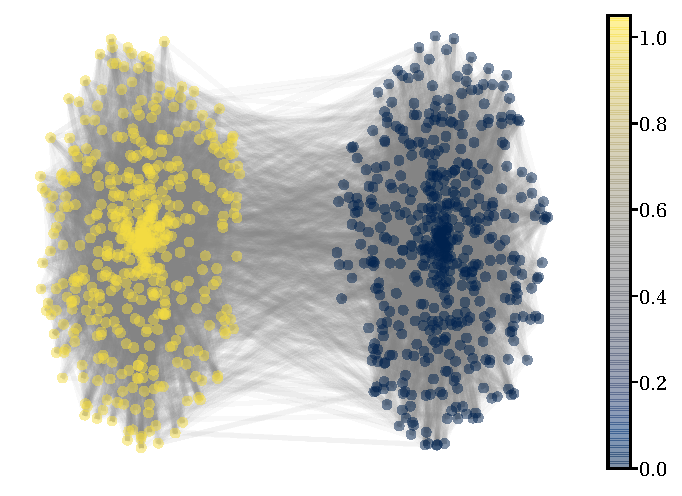
\includegraphics[width=0.48\textwidth]{2ssbm.pdf}}
    \hfill
    \subfloat[Unbalanced 2-\texttt{SBM}(200~+~800)]{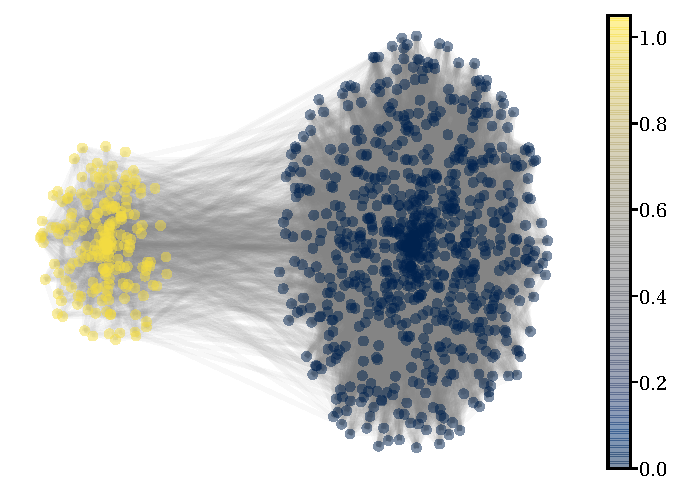
\includegraphics[width=0.48\textwidth]{2sbm.pdf}}
    \caption[Graphs from 2-\texttt{SSBM}(500~+~500) and 2-\texttt{SBM}(200~+~800)]{Graphs drawn from the \acrshort{sbm}$\left(1000, 2, 4.5 \frac{\log (1000)}{1000}, 0.5 \frac{\log (1000)}{1000}\right)$ model, varying the relative community sizes. The vertex colors represent the indicator vector of the leftmost community.}
    \label{fig:2ssbm_and_2sbm}
\end{figure}

My use of community indicator vectors is inspired by one of the basic questions in the study of \acrlongpl{sbm}: can one retrieve the community partitions by looking at the edge structure of graphs drawn from the distribution? Researchers like Abbe~\etal~\cite{abbe2015, abbe2018} have used the \acrfull{map} estimator as a tool prove when this question can be answered. Theorem \ref{thm:exact_recovery_sbm} shows this solvability threshold for the parameters of the 2-\texttt{SSBM}.

\clearpage

\begin{theorem}[\protect{\cite[Thm. 7.1]{abbe2018}}]
    Exact recovery in the symmetric \acrshort{sbm}$\left(n, 2, a \frac{\log n}{n}, b \frac{\log n}{n}\right)$ is solvable if and only if
    \begin{equation}
        \left(\sqrt{a} - \sqrt{b}\right)^2 > 2.
    \end{equation}
    \label{thm:exact_recovery_sbm}
\end{theorem}

To retrieve the community partitions, the graphs drawn from the \acrshort{sbm} distribution have to be at least \emph{connected}~\footnote{Recall from Chapter~\ref{ch:graphs_signals_sampling} that a graph is connected if one can visit all the vertices by travelling only on the edges of the graph.}. Abbe \cite{abbe2018} points out that $a + b > 2$ is the parameter regime for which the 2-\texttt{SSBM} graphs are connected with high probability. The theorem above implies then that $2(\sqrt{ab} - 1)$ is the extra factor needed to go from connectivity to exact recovery. But Abbe's result concerns retrieving the community partitions when all we can observe is the edge structure of the \acrshort{sbm} graphs. When I sample the community indicator vectors, I effectively call upon an oracle to reveal the true assignment of certain vertices. How does the recovery error of the \acrshort{gtv} interpolation \eqref{eq:l1_interpolation} behaves for \acrshort{sbm} distributions with parameter regimes in the neighborhood of the one from Theorem~\ref{thm:exact_recovery_sbm}?

Figure \ref{fig:pt_2ssbm_unif_samp_tv_interp_with_thresholds} shows an initial answer to that question for the 2-\texttt{SSBM}. There, I use uniform random sampling (with replacement) to query the vertex community assignments. The number of measurements varies from zero to the number of vertices~\footnote{Note however that since the sampling is with replacement a number of measurements equal to the number of vertices does not have to yield zero recovery error because there can be redundant samples.}. On the vertical axis, I vary the intra-community connection parameter $a$, starting from the connectivity regime ($a + b > 2$) --- in the bottom --- and passing by the solvability regime from Theorem~\ref{thm:exact_recovery_sbm} --- in the middle. The higher up on the vertical axis, the more dense each community tends to be in terms of number of edges. The average number of edges connecting vertices between different communities stays the same throughout. I measure the recovery error as a normalized~\footnote{The normalization factor is the inverse of the Euclidean norm of the ground-truth signal.} Euclidean distance between the signal estimated by \eqref{eq:l1_interpolation} and the ``ground-truth'' indicator vector. The plot to the right of the figure is a quantized version of the one to the left, presented so that we can better distinguish the level sets in the recovery error.

\begin{figure}[ht]
    \centering
    \subfloat[Recovery error (normalized Euclidean distance)]{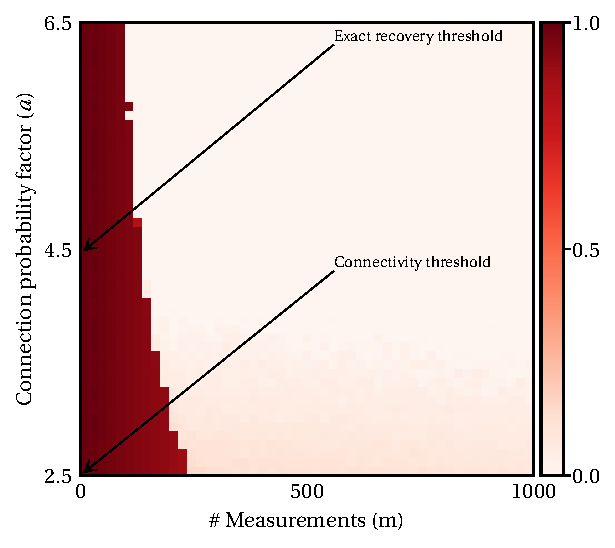
\includegraphics[width=0.48\textwidth]{pt_2ssbm_unif_samp_tv_interp_with_thresholds.pdf}}
    \hfill
    \subfloat[Quantized version]{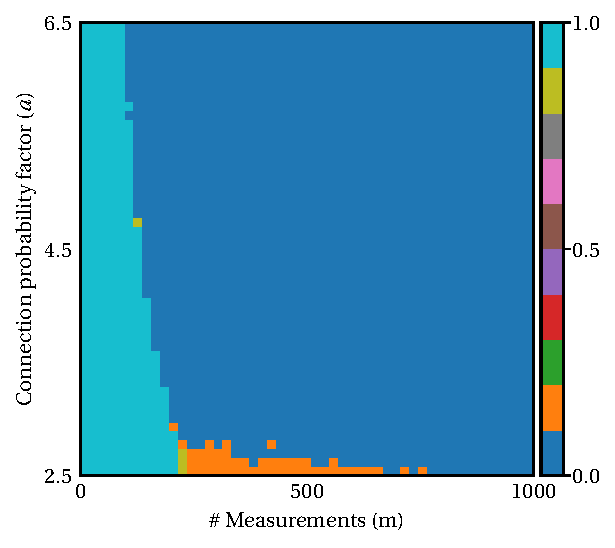
\includegraphics[width=0.48\textwidth]{pt_2ssbm_unif_samp_tv_interp_quantized.pdf}}
    \caption[Phase transition of the recovery error in 2-\texttt{SSBM}(500~+~500) graphs]{Phase transition for the error of \eqref{eq:l1_interpolation} in recovering the community indicator vector of graphs drawn from the symmetric \acrshort{sbm}$\left(1000, 2, a \frac{\log (1000)}{1000}, 0.5 \frac{\log (1000)}{1000}\right)$ from uniform random samples. Each pixel represents the median recovery error across 25 independent trials.}
    \label{fig:pt_2ssbm_unif_samp_tv_interp_with_thresholds}
\end{figure}

Note the clear phase transition when the number of samples reaches a critical value. The threshold happens earlier the higher up on the plot, where the number of edges within the communities becomes progressively larger (on average) than the size of the indicator vector's jump-set. But even the bottom half of the plot exhibits very small recovery errors. This observation does not contradict Theorem \ref{thm:exact_recovery_sbm} --- of course --- but simply attests to the extra information included in the measurements themselves. To allow comparisons with this initial plot, the remaining \acrshort{sbm} experiments in this chapter employ the \acrshort{sbm}$\left(1000, 2, a \frac{\log (1000)}{1000}, 0.5 \frac{\log (1000)}{1000}\right)$ distributions within the same parameter range, \ie with $a$ taking values in the interval $[2.5, 6.5]$.

\subsection{Department indicator vectors in \texttt{email-EU-core}}

The \texttt{email-EU-core} data~\footnote{\url{http://snap.stanford.edu/data/email-Eu-core.html}} represents some email exchanges by people from a large European research institution~\cite{yin2017}. The institution is split into 42 departments, and each of the 1005 individuals in the dataset belongs to exactly one such department. An edge of unitary weight connects two people in the network if they exchanged at least one email. As one could expect, communication tends to stay restricted to within departments, so the network clusters are a reflection the departmental makeup. Thus, the department indicator vectors have small jump sets, as edges across departments are fewer than within. But the number of people in each department is relatively small, so to be fairer with the baseline uniform sampling design I pick as ``ground-truth'' signal for the \texttt{email-EU-core} dataset the indicator vector of the union of the five largest departments. In doing so, the ground-truth takes value $1$ at about 38\% of the vertices and value $0$ at the rest 62\%.

\subsection{Party indicator vectors in \texttt{swiss-national-council}}

I construct the \texttt{swiss-national-council} with data extracted from the 50\textsuperscript{th} legislature in the Swiss Database of Parliamentary Votes~\footnote{\url{https://www.parlament.ch/en/ratsbetrieb/abstimmungen/abstimmungs-datenbank-nr}}. I associate each council member to a feature vector indicating how they voted in each of 3395 affairs accounted for at the time of writing. If they voted \texttt{Yes} in some affair, the corresponding entry in the feature vector receives value $1$; if they voted \texttt{No} the entry gets value $-1$. Affairs for which the councillor did not register a vote (whatever the reason) get a value of $0$. The idea underneath this numerical translation is to use the feature vectors to compare the voting patterns of different council members. Investigating which metric is best for this task is beyond the scope of this thesis, so I opt for the traditional Euclidean distance.

The graph construction takes place directly at the level of the weighted adjacency matrix. Let $\mathbf{f}_i$ and $\mathbf{f}_j$ the the feature vectors of councillors $i$ and $j$. These councillors are then connected with edge weight $W_{ij} = \exp \left ( -\| \mathbf{f}_i - \mathbf{f}_j \|_2^2 / \sigma \right )$, where $\sigma$ is set as the mean distance between feature vectors in the dataset.~\footnote{Exponential kernels such as this are commonly used in Machine Learning and Data Science for similarity computations. The exponential always outputs positive similarity values, and the negative exponent ensures that these values decay quickly towards zero as the feature vectors within become more distant.} Then, to enforce a sparse graph, I keep only the 25 largest edge weights for each council member, setting the rest to $0$ (while making sure that the weight matrix remains symmetric). In the end, councillors that voted identically throughout all the affairs get a unitary edge weight, whereas members that voted differently enough are disconnected.

To put a signal on this graph, I went over the Swiss Parliament files listing the party affiliations of all councillors since 1848.~\footnote{https://www.parlament.ch/en/ratsmitglieder} Intuition tell us that members of the same party stand to vote more similarly than people from different parties. So the party indicator vectors should strongly correlate with the cluster structure of the graph I have constructed. I decided to use as ``ground-truth'' for the experiments the indicator vector of the two largest right-wing parties in the 50\textsuperscript{th} legislature, UDC and FDP. By joining these two parties, the ground-truth signal takes value $1$ at around 46\% of the vertices and $0$ at the other 54\%, an almost even split of the National Council that improves the chances of recovery under uniform random sampling. Meanwhile --- because the two joined parties are to the right in political spectrum --- this concocted ground-truth should still have a sparse jump-set, since the members of UDC and FDP have different voting patterns than the mostly centrist and left-wing politicians in the other half of the Council.

\subsection{Image segmentation masks in \texttt{BSDS300}}

The Berkeley Segmentation Dataset and Benchmark~\footnote{\url{https://www2.eecs.berkeley.edu/Research/Projects/CS/vision/bsds/}} contains 300 images, split into train (100)  and test (200) sets. Each of these images is accompanied by human-generated segmentation masks. What I call the \texttt{BSDS300} dataset is a collection of graphs for each of the 300 images, along with vector representations of the segmentation masks --- interpreted as graph signals.

The first step to construct a graph for each image is to identify each pixel in the image with a vertex in the graph.~\footnote{To get graphs of manageable size for the experiments, I actually subsample the original images by a factor of 12 before starting the graph construction. That is, I keep every 12th row and column of the original image, and use the pixels of this lower-resolution version as the vertices of the graph.} Then, I connect --- with unitary edge weights --- pixels that are adjacent \emph{in the image}. This first set of connection encodes ``spatial similarity'': neighboring pixels in the image are neighbors in the graph. The next set of connections encodes color information via ``patch similarity''. To understand it, let $\mathbf{p}_i \in \mathbb{R}^{147}$ be a vectorized, $7 \times 7 \times 3$ patch containing the RGB values in the image neighborhood centered at pixel $i$.~\footnote{If $i$ is a border pixel, use some form of padding to obtain the patch.} These color patches are used as feature vectors in a the same way as voting data was in the construction of the \texttt{swiss-national-council} graph. I compute edge weights $W_{ij} = \exp \left ( -\| \mathbf{p}_i - \mathbf{p}_j \|_2^2 / \sigma \right )$ for each pair of pixels $i$ and $j$, with $\sigma$ set as the mean patch distance in the image. For the sake of a sparse graph, I then set most of these weights to zero, except for the 3 largest attached to each pixel.~\footnote{This is approximately what happens, because the weight matrix has to be symmetric as well in the end.} The final step is to add the ``spatial'' and ``patch'' weight matrices, whose result represents a hybrid graph that connects pixels either because they are next to each other in the original image grid or because they are the center of similar color patches.

Each segmentation mask in the Berkeley dataset is seen as a piecewise-constant signal for the graph of the image that the mask segments. Step-by-step, I assign an arbitrary integer to each segment in the mask. Then --- for example ---, if a pixel in the original image belongs to segment number 7, its corresponding vertex in the graph gets signal value $7$. This process goes for each vertex, until we have a piecewise-constant graph signal that represents the segmentation of the original image. This signal should have a corresponding small jump-set, because the spatial and color information encoded in the graph structure should correlate with the image segmentation. After all, humans often select as segments continuous objects with homogeneous colors. The edges connecting pixels within the same segment should then be more numerous than the ones across.

\subsection{Data summary}

For future reference, the table on the next page summarizes some key characteristics of the datasets used in this chapter. The number of vertices in the \acrshort{sbm} models is fixed, but since they represent distributions of random graphs, I give their corresponding edge counts as expected values. There is a range to these expected values because I use \acrshort{sbm} models with varying intra-community connection probabilities. The \texttt{BSDS300} line is particular in the sense that there is a different ground-truth signal for each image in the dataset, hence the range of values in the number of edges in the signal's jump-set. As a final note, the complete, undirected graph on 1000 vertices has 499500 edges, so all the graphs in these four datasets are comparatively edge-sparse.

\clearpage
\begin{landscape}
    \centering
    \captionsetup{type=table}
    \begin{tabularx}{\linewidth}{p{4.5cm} r r p{5.0cm} r}
        \hline
        Dataset & Number of vertices & Number of edges & Signal to be recovered & Edges in the jump-set \\
        \hline
        \texttt{2-SSBM}(500~+~500) & 1000 & 5172 -- 12066 & Indicator vector of one of the communities & 863 \\
        \texttt{2-SBM}(200~+~800) & 1000 & 6416 -- 15796 & Indicator vector of the smallest community & 553 \\
        \texttt{email-EU-core} & 1005 & 16064 & Indicator vector of the five largest departments & 4581 \\
        \texttt{swiss-national-council} & 228 & 4259 & Indicator vector of the two largest right-wing parties & 641 \\
        \texttt{BSDS300} & 1107 & 2977 -- 5198 & Segmentation mask & 102 -- 2617 \\
        \hline
    \end{tabularx}
    \captionof{table}[Summary of the data used in the numerical tour]{Summary of the data used in our numerical tour. The edge counts for the \acrshort{sbm} rows are expected values for the parameter regime considered in the experiments.}
\end{landscape}
\clearpage

\section{\texorpdfstring{\acrfull{gtv}}{Graph Total Variation} vs. Dirichlet form}

In Chapter \ref{ch:recovery_convex}, I argued for minimizing the \acrshort{gtv} semi-norm $\|\mathbf{Dz}\|_1$ against the the Dirichlet form $\| \mathbf{Dz} \|_2^2$ in the recovery of piecewise-constant signals. Back then, I used representer theorems to show that the solutions of \acrshort{gtv} decoders depend less on the measurement matrix than their Dirichlet form counterparts. Here I will reinforce this argument by plotting how the recovery error in the two settings varies as we increase the number of vertex measurements that we take. To control for the sampling design, the sampled vertices are always chosen uniformly at random (with replacement) throughout this section.

Let us look first at the behavior of error when recovering the community indicator vector on \acrshort{sbm} graphs. Figure \ref{fig:pt_2sbm_unif_samp_tv_vs_dirichlet} shows the difference between \acrshort{gtv} and Dirichlet form interpolation considering unbalanced 2-\texttt{SBM}(200 + 800) graphs. Similarly to the first \acrshort{sbm} plot in Figure~\ref{fig:pt_2ssbm_unif_samp_tv_interp_with_thresholds}, the vertical axes vary the intra-community connection probability --- moving upwards yields denser communities ---, and the horizontal axes vary the number of uniform random samples of the signal. On the one hand, there is a sharp phase transition on the \acrshort{gtv} column, reminiscent of the one in Figure~\ref{fig:pt_2ssbm_unif_samp_tv_interp_with_thresholds} for the \texttt{2-SSBM}(500~+~500) dataset. But this time the transition curve is more to the right, a consequence of the size imbalance in the communities of \texttt{2-SBM}(200~+~800). Under uniform random sampling, one needs to sample more often to get enough information on the smallest community. On the other hand, the recovery error in the Dirichlet form column decreases smoothly as one gathers more and more samples. Even if its error level-sets are almost indifferent to the density of connections within the communities, their smooth decrease is not fast enough to reach the lowest error levels of the \acrshort{gtv} plot. All in all, \acrshort{gtv} interpolation seems to rely more on the contrast between the ground-truth's jump-set and rest of the edges in the graph; what impacts most the Dirichlet form decoder are the measurement constraints.

\begin{figure}[H]
    \centering
    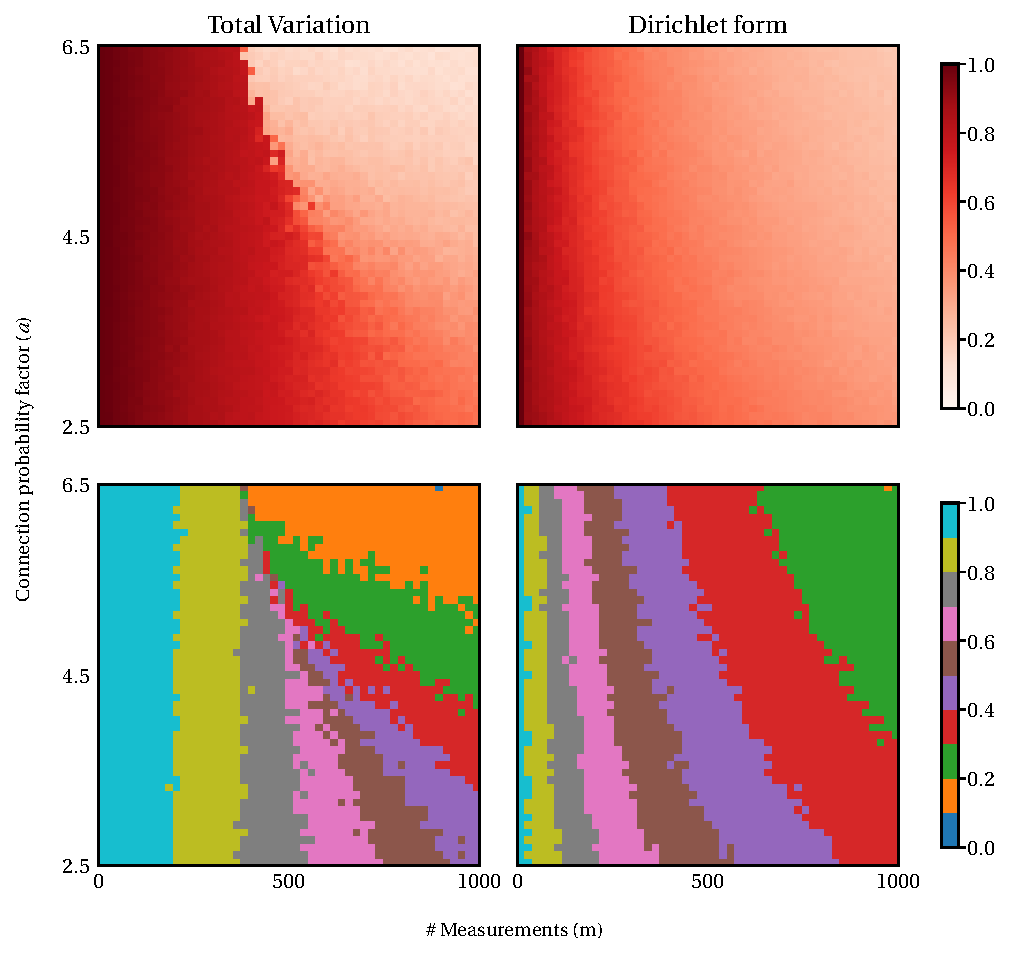
\includegraphics[width=0.95\textwidth]{pt_2sbm_unif_samp_tv_vs_dirichlet.pdf}
    \caption[Decoder's objective and the interpolation error: \texttt{2-SBM}(200~+~800)]{Effect of the decoder's objective on the interpolation error when recovering the indicator vector of the smallest community on \texttt{2-SBM}(200~+~800) graphs from samples taken uniformly at random. Left column: $\|\mathbf{Dz}\|_1$ (\acrlong{gtv} semi-norm). Right column: $\|\mathbf{Dz}\|_2^2$ (Dirichlet form). Each pixel on the top row represents the median, across 25 independent trials, of the normalized Euclidean distance from the recovered vector to the ground-truth. The bottom row has quantized versions of the plots from the top row, to better discern the error level-sets.}
    \label{fig:pt_2sbm_unif_samp_tv_vs_dirichlet}
\end{figure}

If we do the same comparison now using the \texttt{swiss-national-council} data, some of the same behaviors arise, but with interesting twists. See Figure \ref{fig:pt_snc_unif_samp_tv_vs_dirichlet}. The \acrshort{gtv} recovery error transitions sharply, but now this happens in two stages. My hypothesis for this behavior is that it is an artifact of the way I assembled the ground-truth signal. Although the UDC and FDP parties have a joint voting pattern that distinguishes them from the rest of the Council, these parties themselves do not vote identically in every affair. I suppose that the first drop in the error comes when the decoder approximately accounts for the largest, UDC component of the ground truth; the second drop would come when enough members of FDP are sampled as belonging to the same signal piece as UDC. The error in Dirichlet form interpolation does not change in stages; it decreases smoothly and is even smaller then the \acrshort{gtv} error in the beginning, just as in the previous experiment. The surprising observation this time is the error curves of the two decoders catching up at some point and proceeding to decrease smoothly at the same rate. The recovery errors to the right of the plot are still considerably large, but this might just be an indication that there are many councillors in the blue part of the ground-truth that vote very similarly to the UDC or FDP members. In other words, the large interpolation error is possibly a consequence of a large jump-set for the ground-truth signal.

\begin{figure}[H]
    \centering
    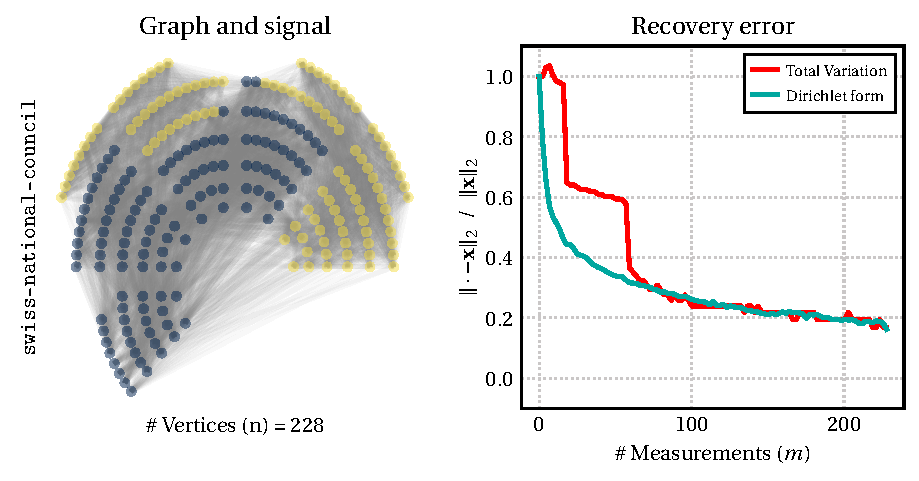
\includegraphics[width=\textwidth]{pt_snc_unif_samp_tv_vs_dirichlet.pdf}
    \caption[Decoder's objective and the interpolation error: \texttt{swiss-national-council}]{Effect of the decoder's objective on the interpolation error when recovering the indicator vector of the two largest right-wing parties (UDC and FDP) in the \texttt{swiss-national-council} graph from samples taken uniformly at random. \textcolor{epfl-groseille}{Red} curve: $\|\mathbf{Dz}\|_1$ (\acrlong{gtv} semi-norm). \textcolor{epfl-canard}{Blue} curve: $\|\mathbf{Dz}\|_2^2$ (Dirichlet form). Each point on the curves represents the median, across 51 independent trials, of the normalized Euclidean distance from the recovered vector to the ground-truth.}
    \label{fig:pt_snc_unif_samp_tv_vs_dirichlet}
\end{figure}


\section{Effects of the sampling design for \texorpdfstring{\acrshort{gtv}}{G-TV} interpolation}

At the end of Chapter \ref{ch:inexact_dual}, I gave an explicit expression for an optimal vertex-sampling design when working with the \acrshort{gtv} interpolation problem \eqref{eq:l1_interpolation}. It prescribes sampling probabilities $\bm{\pi}$ that minimize $\Gamma(\mathcal{S}, \bm{\pi})$, a functional that also depends on the jump-set $\mathcal{S} := \operatorname{supp}\left ( \mathbf{Dx} \right )$ of the signal-to-be-recovered. This optimization program is easy to state, but hard to implement, all due to the indirect definition of the objective as $\Gamma (\mathcal{S}, \bm{\pi}) := \max \{ \Theta (\mathcal{S}, \bm{\pi}), \Upsilon (\mathcal{S}, \bm{\pi})\}$. Out of the two random matrix moment estimates in the definition of $\Gamma$, it is $\Theta$ the one with the simplest expression. I will thus ignore $\Upsilon$ in this section and investigate sampling designs that minimize different upper bounds to $\Theta$, comparing their behavior with the baseline uniform random sampling.

To define the designs we will enquire into, recall Definition~\ref{def:sample_complexity_parameters} and consider the following succession of upper bounds for $\Theta(\mathcal{S}, \bm{\pi})$:
\begin{align}
    \Theta (\mathcal{S}, \bm{\pi}) & = \underset{i \in [n]}{\max} \enspace \underset{k \in [N]}{\max} \enspace \left \| \tilde{\mathbf{e}}_k^{\top} \left [ \mathbf{D} \left ( \mathbf{I}_n - \frac{1}{\pi_{i}}\mathbf{e}_{i} \mathbf{e}_{i}^\top \right ) \mathbf{D}^{+} \right ]^\top \mathbf{P}_{\mathcal{S}}\right \|_{1} \nonumber \\
    & \leq \underset{k \in [N]}{\max} \enspace \left \| \tilde{\mathbf{e}}_k^{\top} \left [ \mathbf{D} \mathbf{D}^{+} \right ]^\top \mathbf{P}_{\mathcal{S}}\right \|_{1} + \underset{i \in [n]}{\max} \enspace \underset{k \in [N]}{\max} \enspace \frac{1}{\pi_i} \left \| \tilde{\mathbf{e}}_k^{\top} \left [ \mathbf{D} \mathbf{e}_{i} \mathbf{e}_{i}^\top \mathbf{D}^{+} \right ]^\top \mathbf{P}_{\mathcal{S}}\right \|_{1} \nonumber \\
    & \leq \sqrt{N} + \underset{i \in [n]}{\max} \enspace \underset{k \in [N]}{\max} \enspace \frac{1}{\pi_i} \left | \tilde{\mathbf{e}}_k^{\top} (\mathbf{D}^{+})^{\top} \mathbf{e}_{i} \right | \cdot \left \| \mathbf{e}_{i}^\top \mathbf{D}^{\top} \mathbf{P}_{\mathcal{S}}\right \|_{1} \nonumber \\
    & = \sqrt{N}  + \underset{i \in [n]}{\max} \enspace \underset{k \in [N]}{\max} \enspace \frac{\left \| (\mathbf{D}^{+})^{\top} \mathbf{e}_{i} \right \|_{\infty} \cdot \left \| \mathbf{P}_{\mathcal{S}} \mathbf{D} \mathbf{e}_{i} \right \|_{1}}{\pi_i} \label{eq:jumpset_coherence_objective}  \\
    & \leq \sqrt{N} + \underbrace{\|\mathbf{P}_{\mathcal{S}} \|_{1 \to 1}}_{= |\mathcal{S}|} \cdot \underset{i \in [n]}{\max} \enspace \underset{k \in [N]}{\max} \enspace \frac{\left \| (\mathbf{D}^{+})^{\top} \mathbf{e}_{i} \right \|_{\infty} \cdot \left \| \mathbf{D} \mathbf{e}_{i} \right \|_{1}}{\pi_i}. \label{eq:naive_coherence_objective}
\end{align}
The sampling design $\bm{\pi}$ minimizing the bound in \eqref{eq:jumpset_coherence_objective} is the one that satisfies
\begin{equation}
    \pi_i = \frac{\left \| (\mathbf{D}^{+})^{\top} \mathbf{e}_{i} \right \|_{\infty} \cdot \left \| \mathbf{P}_{\mathcal{S}} \mathbf{D} \mathbf{e}_{i} \right \|_{1}}{\sum_{j=1}^{n} \left \| (\mathbf{D}^{+})^{\top} \mathbf{e}_{j} \right \|_{\infty} \cdot \left \| \mathbf{P}_{\mathcal{S}} \mathbf{D} \mathbf{e}_{j} \right \|_{1}}, \forall i \in [n].
    \label{eq:jump_set_coherence_probabilities}
\end{equation}
I call it the ``\emph{jump-set coherence}'' design, because it depends on the jump-set $\mathcal{S}$ --- through $\mathbf{P}_{\mathcal{S}}$ --- and on the coherence~\footnote{I use ``coherence'' here in the sense of \acrlong{cs}.} between $\mathbf{D}$ and the standard basis vectors in $\mathbb{R}^{n}$.~\footnote{Recall that our sampling matrix is a stack of standard basis vectors, so the quantified coherence is really between the analysis and measurement operators.} Note that this design is not necessarily practical, since it requires --- \emph{a priori} --- knowing the jump-set of the ``ground-truth'' graph signal. Another sampling design arises when we minimize the the looser bound in \eqref{eq:naive_coherence_objective}:
\begin{equation}
    \pi_i = \frac{\left \| (\mathbf{D}^{+})^{\top} \mathbf{e}_{i} \right \|_{\infty} \cdot \left \| \mathbf{D} \mathbf{e}_{i} \right \|_{1}}{\sum_{j=1}^{n} \left \| (\mathbf{D}^{+})^{\top} \mathbf{e}_{j} \right \|_{\infty} \cdot \left \| \mathbf{D} \mathbf{e}_{j} \right \|_{1}}, \forall i \in [n].
    \label{eq:naive_coherence_probabilities}
\end{equation}
It no longer depends on the jump-set of $\mathbf{x}$, but still has the coherence terms. I name this design ``\emph{naive coherence}'', because it is a consequence of naively controlling the jump-set $\mathcal{S}$ via its cardinality. Getting rid of the jump-set, though, has practical benefits: as long as we know the graph (represented in $\mathbf{D}$) we can implement the \emph{naive coherence} design. There is no need to consider the inaccessible ground-truth signal. But there are other designs that are simple to implement; uniform random sampling being arguably the simplest. \emph{Naive coherence} sampling only makes sense for our purposes if it implies a successful \acrshort{gtv} interpolation using fewer measurements than under uniform random sampling, and not many more than under the \emph{jump-set coherence} design. I contrast these three sampling strategies --- summarized on Table \ref{tab:summary_sampling_designs} --- in the set of experiments that follows.

\begin{table}[H]
    \centering
    \begin{tabularx}{0.6\textwidth}{rl}
        \hline
        Sampling design & Expression ($\forall i \in [n]$) \\
        \hline
        Uniform & $\pi_i = 1/n$ \\
        Naive coherence & $\pi_i \propto \left \| (\mathbf{D}^{+})^\top \mathbf{e}_i \right \|_{\infty} \cdot \left \| \mathbf{D} \mathbf{e}_i \right \|_1$ \\
        Jump-set coherence & $\pi_i \propto \left \| (\mathbf{D}^{+})^\top \mathbf{e}_i \right \|_{\infty} \cdot \left \| \mathbf{P}_\mathcal{S} \mathbf{D} \mathbf{e}_i \right \|_1$ \\
        \hline
    \end{tabularx}
    \caption[Summary of the three sampling designs compared in the experiments]{Summary of the sampling designs compared in the experiments. The expressions refer to the sampling probabilities $\bm{\pi} = (\pi_1, \dots, \pi_n)$ used in the \acrshort{cswr} model for vertex-sampling of graph signals (see Section~\ref{sec:sampling}).}
    \label{tab:summary_sampling_designs}
\end{table}

Let us begin by revisiting the \acrshort{sbm} datasets. Figure \ref{fig:pt_2sbm_tv_interp} shows the recovery error of \acrshort{gtv} interpolation under the three sampling designs, contrasting balanced and unbalanced community settings. We have already seen the plots from first column, but note how similar they are with the ones from the second column. The sample complexity for a correct output in \eqref{eq:l1_interpolation} under \emph{naive coherence sampling} is the same as if the vertices were sampled uniformly at random. The naive control over the ground-truth's jump-set is not enough to change the phase transition profile, a conclusion made all the more convincing once we examine the figure's third column. The change is subtle for the balanced \texttt{2-SSBM}(500~+~500) dataset, but very pronounced for the unbalanced case. Recovering the indicator vector unbalanced \texttt{2-SBM}(200~+~800) graphs is the naturally hard setting for the uniform sampling strategy, since the sampled vertices have only a one-in-four chance of belonging to the smallest community; in the balanced graphs, every other sample belongs to either community. The \emph{jump-set coherence} design seems to regularize the unbalanced signals, making the phase transition of their recovery look like the one for the symmetric \acrshort{sbm} under \emph{uniform random sampling}. The underlying cause of this regularization is found upon examining expression \eqref{eq:jump_set_coherence_probabilities}: only the vertices connected to edges on the ground-truth's jump-set are sampled with probability larger than zero.

\clearpage
\begin{figure}
    \centering
    \subfloat[\texttt{2-SSBM}(500~+~500)]{
        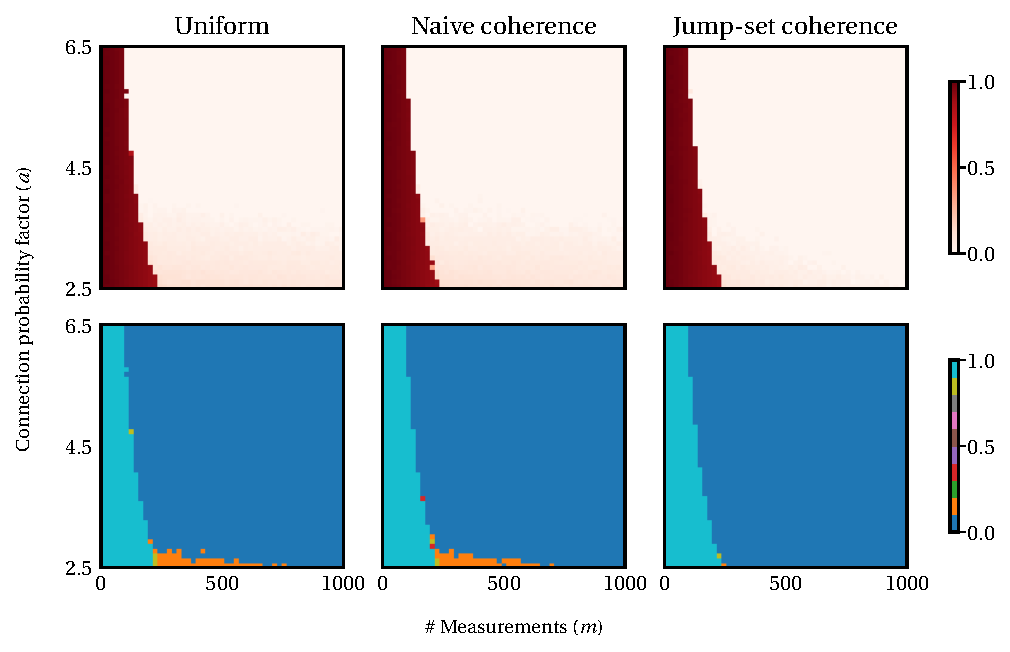
\includegraphics[width=0.95\textwidth]{pt_2ssbm_tv_interp.pdf}
    }
    \hfill
    \subfloat[\texttt{2-SBM}(200~+~800)]{
        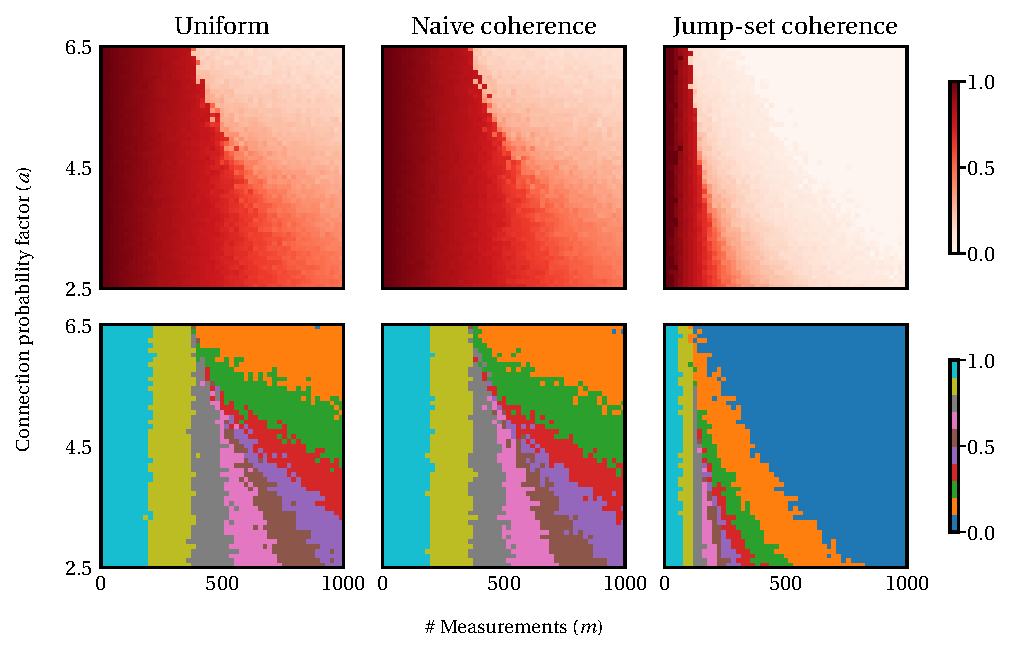
\includegraphics[width=0.95\textwidth]{pt_2sbm_tv_interp.pdf}
    }
    \caption[Three sampling designs: \texttt{2-SSBM}(500~+~500) and \texttt{2-SBM}(200~+~800)]{Impact of three sampling designs on the recovery error of \acrshort{gtv} interpolation for the community indicator vectors of \acrshort{sbm} graphs. Each pixel represents the median error over 25 independent trials. Each plot is paired with its quantized version highlighting some error level-sets.}
    \label{fig:pt_2sbm_tv_interp}
\end{figure}
\clearpage

We can draw similar conclusions for the effects of the three sampling designs using the ``real-world'' datasets \texttt{email-EU-core} and \texttt{swiss-national-council}, but we find also some surprises. Figure~\ref{fig:pt_email_snc_tv_interp} shows that once again the \emph{naive coherence} design behaves just as poorly as \emph{uniform random sampling}; the red curves are more intriguing.

\begin{figure}[H]
    \centering
    \subfloat[Ground-truth: indicator vector of the 5 largest departments]{
        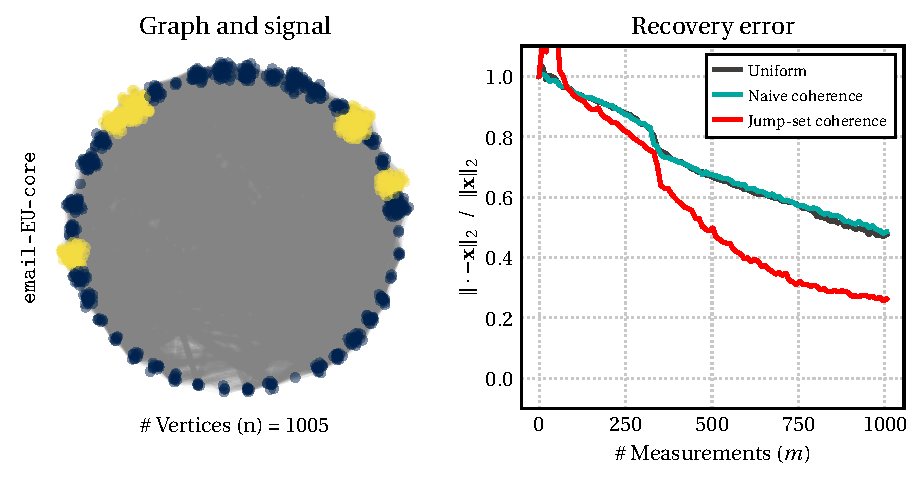
\includegraphics[width=0.95\textwidth]{pt_email_eu_core_tv_interp.pdf}
    }
    \hfill
    \subfloat[Ground-truth: indicator vector of the 2 largest right-wing parties]{
        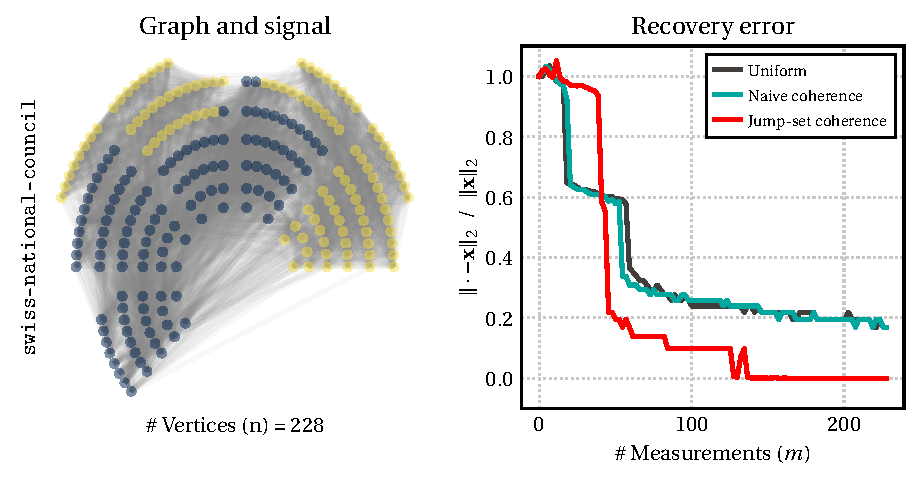
\includegraphics[width=.9\textwidth]{pt_snc_tv_interp.pdf}
    }
    \caption[Three sampling designs: \texttt{email-EU-core} and \texttt{swiss-national-council}]{Impact of three sampling designs on the recovery error of \acrshort{gtv} interpolation for the signals of the \texttt{email-EU-core} and \texttt{swiss-national-council} datasets. Each point in the plot represents the median error over 51 independent trials.}
    \label{fig:pt_email_snc_tv_interp}
\end{figure}
\clearpage

On the plots of Figure~\ref{fig:pt_email_snc_tv_interp}, the \emph{jump-set coherence design} reaches smaller recovery errors than the ones of the two others, but when the measurements are very few this design's error becomes the largest. I think this has do with with how well the ground-truth's jump-set reflects the natural partitions of the graph. When the \acrshort{gtv} decoder has very few measurements, it must rely almost only on the graph structure to do the interpolation. For the \acrshort{sbm} datasets this dependence was not detrimental because the signals being recovered were really the indicator vectors of the natural communities in the graphs. For the \texttt{email-EU-core} and \texttt{swiss-national-council} datasets I constructed assembled the ground-truth based only on an intuitive idea of how the respective graphs would cluster. When sampling a few vertices, only at the signal transitions, the \emph{jump-set coherence design} may lack the sample variety of the other designs that suggests the \acrshort{gtv} decoder should settle for a less-than-natural partition of the graph. In the end, however, the role of the graph in recovery problems like ours is to \emph{inform} the composition of the signal; very rarely in practice does the graph encode \emph{exactly} a signal of interest. The fact that the \emph{jump-set coherence design} reaches --- globally --- lower error levels than the other two designs is more important. After all, the error values to the left of the plot are \emph{all} very large. To the right --- as the number of samples increases---, the \emph{jump-set coherence design} even results in exact recovery for the \texttt{swiss-national-council} data, hinting that the voting patterns of the Swiss National Councillors reflect their political leaning better than the email exchanges in the \texttt{email-EU-core} reflect the institution's departmental makeup.

To finish off, let us sweep the \texttt{BSDS300} dataset and compare the error curves for the three sampling designs when recovering the segmentation mask graph signals. Figure \ref{fig:pt_bsds300_tv_interp} displays these side-by-side, with a gray curve for each image in the dataset.

\begin{figure}[H]
    \centering
    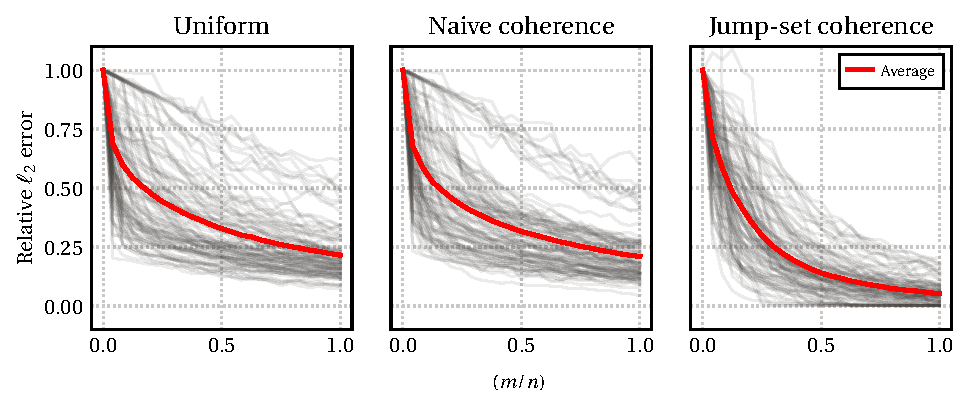
\includegraphics[width=\textwidth]{pt_bsds300_tv_interp.pdf}
    \caption[Three sampling designs: \texttt{BSDS300}]{Impact of three sampling designs on the recovery error of \acrshort{gtv} interpolation for the segmentation masks in \texttt{BSDS300}. Each grey curve on each of the three plots corresponds to an image in the dataset. Each point in these curve records the median error over 15 independent trials. The red curve traces the point-wise average the grey ones.}
    \label{fig:pt_bsds300_tv_interp}
\end{figure}

Note first that not every image in the dataset admits a sharp phase transition in the recovery error. For some, the error drops suddenly at a critical number of samples; for others the error decreases smoothly and remains large even when a lot of pixels are queried. For the first time in our experiments one could argue that there is \emph{some} improvement in using the \emph{naive coherence design} over uniform random sampling, but not enough to justify its use. The \emph{jump-set coherence design} leads to exact recovery for some segmentation masks, but for others the recovery error remains fairly large despite the use of unfair knowledge about the ground-truth jump-set in the sampling design. Let us examine the images associated with extremes of this behavior to see where this disparity comes from. The left column of Figure~\ref{fig:bsds300_imgs_smallest_largest_error} shows the image whose segmentation mask leads to the smallest recovery error under \emph{jump-set coherence sampling}; the right column shows the image with the largest respective error. The larger error seems to have to do with with the presence of several small pieces in the image's segmentation. Even when the sampling design is restricted to query only vertices belonging to the jump-set, it can still miss samples from some of the several small segments.

\begin{figure}[H]
    \centering
    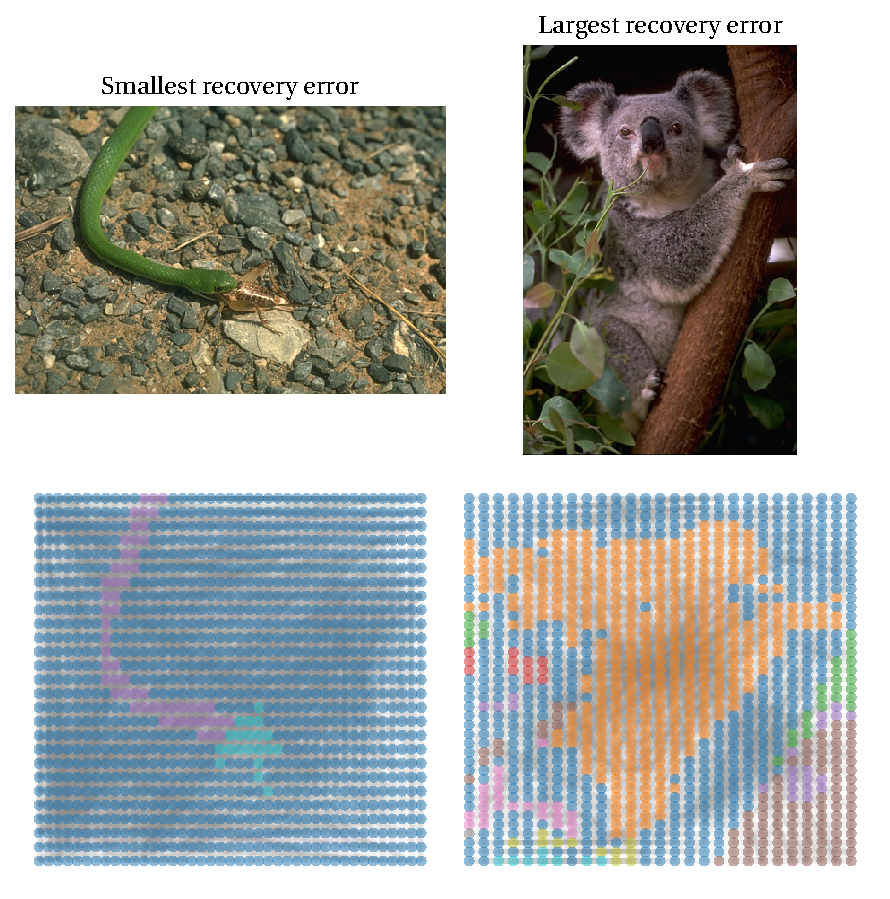
\includegraphics[width=0.7\textwidth]{bsds300_imgs_smallest_largest_error.pdf}
    \caption[Segmentation masks in \texttt{BSDS300} with the smallest and largest recovery errors]{Segmentation mask signals in the \texttt{BSDS300} dataset that yield the smallest and largest recovery errors when taking $m = n$ samples (with replacement) under the \emph{jump-set coherence design}.}
    \label{fig:bsds300_imgs_smallest_largest_error}
\end{figure}
\clearpage


\section{Summary}

The thorough study of a recovery program should not ignore the issues involved in its practical use. Fortunately, the \acrshort{gtv} decoders in \eqref{eq:l1_interpolation} and \eqref{eq:l1_regression} can be implemented numerically in efficient ways. The one I presented is based on a single primal-dual proximal splitting procedure whose iterations required, in the end, operations that can be made cheaper the sparser the graph is. Upon convergence, the estimated solution can be close or far to the true underlying signal, depending on the number of vertex-samples taken. I have shown that when the ground-truth is the indicator vector of a graph cluster, the recovery error of \acrshort{gtv} interpolation undergoes a sharp phase transition with respect to the number of samples. The threshold happens earlier the denser are the clusters. In contrast, the error under Dirichlet form interpolation when recovering these signals decreases smoothly and slowly, depending more on the actual number of measurements than on the edge structure of the graph.

Putting into practice the optimal sampling design for \acrshort{gtv} interpolation also has issues of its own. In an effort to simplify the complicated objective of the optimal design, I proposed for it two progressively looser upper bounds, whose optimizers gave rise to two sampling designs. Both are a form of coherence sampling, familiar in \acrlong{cs}, but one of them also uses information from the jump-set of the ground-truth signal. I compared these two designs with the baseline uniform random sampling, concluding that some information about the ground-truth's jump-set must be used in order to change the phase transition profile of the recovery error in \acrshort{gtv} interpolation; \emph{naive coherence sampling} behaves just as poorly as \emph{uniform random sampling}. The practical issue that remains is how to account for the jump-set in the sampling designs without actually resorting to the --- \emph{unknowable} --- ground-truth signal?

\clearpage

\begin{subappendices}
    \section{More on primal-dual proximal splitting}\label{ap:primal_dual_prox_split}
    In this appendix I sketch, in a little more detail than in the main text, the proximal splitting approach for numerically solving programs like the \acrshort{gtv} decoders \eqref{eq:l1_interpolation} and \eqref{eq:l1_regression}. We may consider here more general optimization problems of the type
\begin{equation}
    \underset{\mathbf{z} \in \mathbb{R}^{n}}{\min} \enspace f(\mathbf{z}) + g(\mathbf{Dz}) + h(\mathbf{z}),
    \label{eq:opt_prob_std_form} \tag{$P_{\text{std}}$}
\end{equation}
where $f: \mathbb{R}^{n} \to \mathbb{R}$, $g: \mathbb{R}^{N} \to \mathbb{R}$ and $h: \mathbb{R}^{n} \to \mathbb{R}$ are convex functions, the latter of which is also differentiable (with a Lipschitz-continuous gradient).

The proximity operator of a convex function $f : \mathbb{R}^{n} \to \mathbb{R}$ is the map
\begin{equation}
    \mathbf{z} \mapsto \operatorname{prox}_{f} \left ( \mathbf{z} \right ) = \text{arg} \enspace \underset{\mathbf{v} \in \mathbb{R}^{n}}{\min} \enspace \frac{1}{2} \|\mathbf{z} - \mathbf{v} \|_2^2 + f(\mathbf{v}).
\end{equation}
The problem on the \acrlong{rhs} admits a unique solution for every $\mathbf{z} \in \mathbb{R}^{n}$. One can interpret proximity operators as generalizing projections. Indeed, take $f$ to be the convex indicator function of a set $\mathcal{C}$, \ie, the functions defined by
\begin{equation*}
    \mathbf{z} \mapsto \iota_{\mathcal{C}}(\mathbf{z}) = \left \{
        \begin{matrix}
            0, & \text{if }\mathbf{z} \in \mathcal{C}, \\
            +\infty & \text{otherwise}
        \end{matrix}
    \right. .
\end{equation*}
Then, for any $\mathbf{z} \in \mathbb{R}^{n}$, the vector $\operatorname{prox}_{f} \left ( \mathbf{z} \right )$ is exactly the orthogonal projection of $\mathbf{z}$ onto $\mathcal{C}$~\cite[Table~2,~entry~i]{combettes2011}. Just like orthogonal projections, proximity maps allow us to split the space into complementary halves. Given a convex function $f$, the so-called Moreau decomposition of any $\mathbf{v} \in \mathbb{R}^{n}$ is given by
\begin{equation*}
    \mathbf{v} = \operatorname{prox}_{f} \left ( \mathbf{v} \right ) + \operatorname{prox}_{f^*} \left ( \mathbf{v} \right ),
\end{equation*}
where $f^*$ is the Fenchel conjugate of $f$, a function defined as $\mathbf{v} \mapsto \underset{\mathbf{u} \in \mathbb{R}^{n}}{\sup} \enspace \langle \mathbf{u}, \mathbf{v} \rangle - f(\mathbf{u})$.

But perhaps the two most important properties of $\operatorname{prox}_{f}$ --- in what concerns iterative solvers --- are its firm non-expansiveness and the fact that its fixed point set matches the set of minimizers of $f$~\cite{combettes2011}. The gradient descent map $\mathbf{w} \mapsto \mathbf{w} - \gamma \nabla h (\mathbf{w})$ can also be non-expansive (with a proper choice of step size $\gamma$) and, similarly to the proximity map, its fixed point set is equal to the set of minimizers of $h$. \emph{Proximal splitting} techniques take advantage of these two properties to solve problems of the type $\underset{\mathbf{z}}{\min} \enspace f(\mathbf{z}) + h(\mathbf{z})$ with alternating calls to the gradient of $h$ (forward step) and proximal operator of $f$ (backward step). In rough terms, the iterations look like the ones below and repeat until $\mathbf{z}$ stops changing noticeably, coming close enough to a minimizer of the sum $f(\cdot) + h(\cdot)$.
\begin{algorithm}[H]
    \begin{algorithmic}
        \State{$\mathbf{z} \gets \mathbf{z} - \gamma \nabla h (\mathbf{z})$}\Comment{Forward step}
        \State{$\ldots$}
        \State{$\mathbf{z} \gets \operatorname{prox}_{\gamma f} \left ( \mathbf{z} \right )$}\Comment{Backward step}
    \end{algorithmic}
\end{algorithm}

Adding $g$ to the objective changes things a bit, because the domain of this function is different from that of $f$ and $h$. \emph{Primal-dual} proximal splitting methods address this situation by working simultaneously with two variables, called the primal $\mathbf{z} \in \mathbb{R}^{n}$ and the dual $\mathbf{d} \in \mathbb{R}^{n}$. The direct linear map $\mathbf{z} \mapsto \mathbf{D}\mathbf{z}$ and its transpose, $\mathbf{d} \mapsto \mathbf{D}^\top \mathbf{d}$ connect the primal and dual domains between the forward and backward steps:
\begin{algorithm}[H]
    \begin{algorithmic}
        \State{$(\mathbf{z}, \mathbf{d}) \gets \left(\mathbf{z} - \gamma \nabla h (\mathbf{z}) - \gamma \mathbf{D}^\top \mathbf{d}, \mathbf{d} + \gamma \mathbf{D} \mathbf{z}\right)$}\Comment{Forward step}
        \State{$\ldots$}
        \State{$(\mathbf{z}, \mathbf{d}) \gets \left(\operatorname{prox}_{\gamma f} \left ( \mathbf{z} \right ), \operatorname{prox}_{\gamma g^*} \left ( \mathbf{d} \right )\right)$}\Comment{Backward step}
    \end{algorithmic}
\end{algorithm}

The specific primal-dual proximal splitting method used in this chapter comes from Komodakis~and~Pesquet~\cite[Algorithm~6]{komodakis2015}. I reproduce all of its steps in Algorithm \ref{algo:primal_dual_general}, but note that at its core the algorithm consists of forward gradient steps, backward proximity steps, and a linear connection between primal and dual spaces via matrix $\mathbf{D}$. The paper of Komodakis~and~Pesquet lists other numerical solvers for \eqref{eq:opt_prob_std_form}, but the one in Algorithm~\ref{algo:primal_dual_general} has more intuitive step size parameters and allows the computation of $\operatorname{prox}_{f}$ and $\operatorname{prox}_{g}$ in parallel.

\begin{algorithm}
    \caption{\acrshort{fbf} primal-dual iterations for solving \eqref{eq:opt_prob_std_form}}
    \label{algo:primal_dual_general}
    \begin{algorithmic}[1]
        \State{$\mathbf{z}_0 \gets \mathbf{0} \in \mathbb{R}^{n}$}\Comment{Initial primal variable}
        \State{$\mathbf{d}_0 \gets \mathbf{0} \in \mathbb{R}^{N}$}\Comment{Initial dual variable}
        \Repeat
            \State{\textbf{pick} $\gamma_n \in \left(0, \frac{1}{1 + \|\mathbf{D}\|_{2} + \rho}\right)$}\Comment{Step size}

            \State{$\left(\mathbf{w}_{1,n},\enspace\mathbf{w}_{2,n}\right) \gets \left(\mathbf{z}_n - \gamma_n \left[\nabla h (\mathbf{z}_n) + \mathbf{D}^\top \mathbf{d}_n\right],\enspace\mathbf{d}_n + \gamma_n \mathbf{D}\mathbf{z}_n\right)$}\Comment{Forward step}

            \State{$\left(\mathbf{p}_{{1,n}},\enspace\mathbf{p}_{{2,n}}\right) \gets \left(\operatorname{prox}_{\gamma_n f} \left ( \mathbf{w}_{1,n} \right ),\enspace\operatorname{prox}_{\gamma_n g^*} \left ( \mathbf{w}_{2,n} \right )\right)$}\Comment{Backward step}

            \State{$\left(\mathbf{q}_{{1,n}},\enspace\mathbf{q}_{{2,n}}\right) \gets \left(\mathbf{p}_{{1,n}} - \gamma_n \left[ \nabla h (\mathbf{p}_{{2,n}}) + \mathbf{D}^\top \mathbf{p}_{{2,n}}\right],\enspace\mathbf{p}_{{2,n}} + \gamma_n \mathbf{D} \mathbf{p}_{{1,n}}\right)$}\Comment{Forward} step

            \State{$\left(\mathbf{z}_{n+1},\enspace\mathbf{d}_{n+1}\right) \gets \left(\mathbf{z}_n - \mathbf{w}_{1,n} + \mathbf{q}_{1,n},\enspace\mathbf{d}_n - \mathbf{w}_{2,n} + \mathbf{q}_{2,n}\right)$}\Comment{Update primal/dual variables}

        \Until{convergence}
        \State{\textbf{return} $\mathbf{z}_{n+1}$}
	\end{algorithmic}
\end{algorithm}

Algorithms \ref{algo:primal_dual_interpolation} and \ref{algo:primal_dual_regression} in the main text are straightforward specializations of Algorithm \ref{algo:primal_dual_general}. To see that this is true, first identify $g$ with $\|\cdot\|_1 : \mathbb{R}^{N} \to \mathbb{R}$. Then the proximal mapping of its Fenchel conjugate is given by
\begin{align*}
    \mathbf{w} \mapsto & \operatorname{prox}_{\gamma_n g^*} \left ( \mathbf{w} \right ) \\
    & = \mathbf{w} - \operatorname{prox}_{\gamma_n g} \left ( \mathbf{w} \right ) \\
    & = \mathbf{w} - \operatorname{soft}_{\gamma_n} (\mathbf{w}).
\end{align*}
Note that I used the Moreau decomposition, along with the fact that $\operatorname{prox}_{\gamma_n \|\cdot\|_1}$ is the soft thresholding operator $\operatorname{soft}_{\gamma_n} (\mathbf{w})$~\cite[Table 2, entry ii]{combettes2011}. Next, in the interpolation problem related to Algorithm~\ref{algo:primal_dual_interpolation}, we have $h \equiv 0$ and so $\nabla h \equiv \mathbf{0}$. The interpolation constraint is expressed via function $f$ with the convex indicator function $\iota_{\{\mathbf{z} \in \mathbb{R}^{n} : \mathbf{P}_{\Omega}\mathbf{z} = \mathbf{P}_{\Omega}\mathbf{x}\}}(\cdot)$. Its proximity map is the same as the orthogonal projection onto set $\{\mathbf{z} \in \mathbb{R}^{n} : \mathbf{P}_{\Omega}\mathbf{z} = \mathbf{P}_{\Omega}\mathbf{x}\}$:
\begin{align*}
    \mathbf{w} \mapsto & \operatorname{prox}_{\gamma_n f} \left ( \mathbf{w} \right ) \\
    & = \text{arg} \enspace \underset{\{ \mathbf{z} \in \mathbb{R}^{n} : \mathbf{P}_{\Omega} \mathbf{z} = \mathbf{P}_{\Omega} \mathbf{x} \}}{\min} \enspace \|\mathbf{z} - \mathbf{w}\|_2 \\
    & = (\mathbf{I}_n - \mathbf{P}_{\Omega}) \mathbf{w} + \mathbf{P}_{\Omega}\mathbf{x}.
\end{align*}
For the regression problem, we can express the constraints using a differentiable function, $h(\cdot) = \frac{\rho}{2} \| \mathbf{P}_{\Omega}(\cdot) - \mathbf{y}\|_2^2$. Its corresponding gradient map is $\mathbf{z} \mapsto \nabla h (\mathbf{z}) = \rho \mathbf{P}_{\Omega}^\top \mathbf{P}_{\Omega}\mathbf{z} - \mathbf{y} = \rho \mathbf{P}_{\Omega}\mathbf{z} - \mathbf{y}$. There is no need for another function in the objective, so we may set $f \equiv 0$, which finishes the specialization of Algorithm \ref{algo:primal_dual_general} into Algorithm~\ref{algo:primal_dual_regression}.
\end{subappendices}
\chapter{Conclusions}

\quote[0.625\textwidth]{I want to stand as close to the edge as I can without going over. Out on the edge you see all kinds of things you can't see from the center.}{Kurt Vonnegut, Player Piano}

To find the missing values, we first connected the dots. Discrete signals are often informed by the similarity of its support points. Groups of friends tend to watch the same movies; politicians that vote alike tend to be in the same party. Those similarities can be concisely represented through a network, and the original signal becomes a graph signal. Still, I have shown in the beginning of this thesis how to express the sampling and analysis of graph signals in the familiar language of linear algebra. The graph gradient matrix, $\mathbf{D}$, arose as the analysis operator for piecewise-constant signals, that is, those that have few edge-variations. Matrix $\mathbf{A}$, representing vertex-sampling, was formed by stacking independent random rows from the standard basis in $\mathbb{R}^{n}$, according to two alternative sampling models --- \acrshort{ber} and \acrshort{cswr}.

To figure the whole from its samples, we exploited a signature feature. For graph signals that are piecewise-constant, a good potential signature is the count of edges across which the signal varies. Among all possible ways to ``count'' the edge differences, I contrasted the \acrfull{gtv} and the Dirichlet form. Both theoretically and numerically, I argued that \acrshort{gtv} minimization is less sensitive to the sampling \emph{operator}. In particular, its recovery error drops suddenly close to zero as long as \emph{the number} of measurements is large enough.

To reveal the best sampling design, we minimized the sample complexity. I explored two approaches to study the recovery conditions under \acrshort{gtv} minimization. The ``direct'' path of Chapter \ref{ch:lower_bound_min_gain} is the more general --- dealing automatically with noisy samples --- but I was forced to leave it without a punchline. What blocked it was the lack of knowledge on the coordinate structure of the decent cone $\mathcal{D} \left ( \|\mathbf{D} \cdot\|_1 , \mathbf{x} \right )$. The ``dual'' path of Chapter \ref{ch:inexact_dual} was more fruitful, revealing the number of measurements required for exact \acrshort{gtv} interpolation as a function of the sampling probabilities $\bm{\pi} =(\pi_1, \dots, \pi_n)$. What followed was an explicit expression for the optimal vector $\bm{\pi}$.

To realize the practical issues, we finally took a numerical tour. Implementing the decoders was fairly easy; implementing the optimal sampling design is less so. Nevertheless, we saw how an approximation of the optimal design can visibly change the phase transition profile of the recovery error in \acrshort{gtv} interpolation. But this approximate design has to depend on the ground-truth signal's jump-set, knowledge of which is unobtainable a priori. Indeed --- for all the different datasets of Chapter~\ref{ch:numerical_tour} ---, the \emph{naive coherence design} behaved just as well as \emph{uniform random sampling}, while the \emph{jump-set coherence} alternative moved the sample complexity threshold towards lower measurement levels.

I leave the readers with two lists that summarize what we have learned in this thesis and what we still have to learn about sampling and subsequent \acrshort{gtv} recovery of piecewise-constant graph signals.

\section{Takeaways}

\begin{itemize}
    \item \textbf{Piecewise-constant signals and the geometry of $\mathbb{B}_{\acrshort{gtv}}$.} The extreme ``points'' of the \acrfull{gtv} ball are essentially indicator vectors of vertex subsets. These indicators are basic elements for a sparse description of piecewise-constant graph functions. On the one hand, the solutions of \acrshort{gtv} minimization will thus tend to be sparse combinations of vertex-subset indicator vectors. On the other hand, the extreme points of the solution set can be \emph{represented} by a selection of columns from the pseudo-inverse $\mathbf{D}^{+}$. Piecewise-constant graph signals that are ``compatible'' with the graph structure require relatively few atoms from $\mathbf{D}^{+}$ in its description. Compatible signals can be potentially recovered by \acrshort{gtv} minimization using only a few vertex samples.
    \item \textbf{Optimal sampling design for \acrshort{gtv} interpolation.} The sampling probabilities that minimize the recovery threshold for \acrshort{gtv} interpolation depend on vertex-induced perturbations of the projection operator $\mathbf{D D}^{+}$, restricted to the jump-set $\mathcal{S} := \operatorname{supp}\left ( \mathbf{Dx} \right )$ of the signal $\mathbf{x}$ to be recovered.
    \item \textbf{Importance of the jump-set in the sample complexity threshold.} Attempting to write the sample complexity of \acrshort{gtv} decoders as simply proportional to the jump-set's cardinality might incur in vacuous bounds. This is true, first, because $|\mathcal{S}|$ in piecewise-constant graph signals can be much larger than the signal's dimension and, yet, these signals can still be successfully recovered from relatively few measurements. Second, a sampling design based on this \emph{naive} control over the jump-set induces the same recovery error profile as if the vertices were sampled uniformly at random.
\end{itemize}

\section{Open problems}

\begin{itemize}
    \item \textbf{A direct certificate for \acrshort{gtv} recovery.} Knowing more about the coordinate structure of the descent cone $\mathcal{D} \left ( \|\mathbf{D} \cdot\|_1 , \mathbf{x} \right )$ --- whenever $\mathbf{x}$ is a piecewise-constant graph signal --- can lead to a high-probability lower bound on the minimum $q$-gain functional. Such a result would be more powerful than the certificate from Chapter \ref{ch:inexact_dual}, because it would imply robustness guarantees for the noisy regression problem \eqref{eq:l1_regression}. In fact, it would even be useful in more general settings where the measurements undergo some non-linear transformation before becoming available~\cite{plan2016}.
    \item \textbf{Practical sampling designs.} The optimization program in Corollary \ref{cor:opt_samp_design} is explicit but not practical a priori. I used a simplified version of it in Chapter \ref{ch:numerical_tour} but even then the sampling design that performed well was the one that demanded knowing the signal-to-be-sampled before even sampling it. We are thus left with a modelling problem. The optimal design depends on the action of the projection operator $\mathbf{P}_{\mathcal{S}}$, but knowing this operator is tantamount to knowing the jump-set $\mathcal{S}$ of the signal we want to recover. How much is it possible to assume, in practice, about the actions of $\mathbf{P}_{\mathcal{S}}$ without explicitly knowing $\mathcal{S}$?
\end{itemize}



%%%%%%%%%%%%%%%%%%%%%%%%%%%%%%%%%%%%
% TAIL: Bibliography, Appendix, CV %
%%%%%%%%%%%%%%%%%%%%%%%%%%%%%%%%%%%%

\begin{appendices}
    \chapter{Bernstein inequalities}\label{ap:probabilistic_inequalities}

Many of the random objects encounter in this thesis can be written as a sum of independent random variables. The terms of the sum have bounded moments, so the sum itself takes on values close to its expectation with high probability. This concentration phenomenon can be quantified in terms of the Bernstein-type inequalities that I present here.

\begin{lemma}[\protect{Scalar Bernstein inequality~\cite[p.117]{artstein-avidan2015}}]\label{lem:scalar_bern}.
    Let $X_1, \dots, X_n$ be \textit{independent} random variables, taking values in $\mathbb{R}$, and such that, for each $i \in [n]$,
    \begin{itemize}
        \item $\mathbb{E} \left ( X_i \right ) = 0$,
        \item $\sigma^2 := \frac{1}{n} \sum_{i=1}^{n} \mathbb{E} \left ( X_i^2 \right ) < \infty$,
        \item $ |X_i| \leq B < \infty$.
    \end{itemize}
    Then, $\forall t > 0,$ the tails of the sum $S_n := X_1 + \dots + X_n$ behave as
    \begin{equation}
        \mathbb{P} \left ( \left \{  |S_n| \geq t n \right \}\right ) \leq 2 \exp \left( \frac{-3 n}{8} \min \left \{ \frac{t^2}{\sigma^2}, \frac{t}{B} \right \} \right).
    \end{equation}
\end{lemma}

\begin{lemma}[\protect{Vector Bernstein inequality~\cite[p.164]{ledoux2011a}}]\label{lem:vector_bern}
    Let $X_1, \dots, X_n$ be \textit{independent} random vectors in a Banach space equipped with norm $\| \cdot \|$, such that, for each $i \in [n]$,
    \begin{itemize}
        \item $\mathbb{E} \left ( X_i \right ) = 0$,
        \item $\sigma^2 := \frac{1}{n} \sum_{i=1}^{n} \mathbb{E} \left ( \|X_i\|^2 \right ) < \infty$,
        \item $ \|X_i\| \leq B < \infty$.
    \end{itemize}
    Then, $\forall t > 0,$ the tails of the sum $S_n := X_1 + \dots + X_n$ behave as
    \begin{equation}
        \mathbb{P} \left ( \left \{  \| S_n \| \geq t n \right \}\right ) \leq 2 \exp \left( \frac{-3 n}{8} \min \left \{ \frac{t^2}{\sigma^2}, \frac{t}{B} \right \} \right).
    \end{equation}
\end{lemma}

\begin{lemma}[\protect{Matrix Bernstein inequality~\cite[Thm. 1.6.2]{tropp2015b}}]\label{lem:matrix_bern}
    Let $X_1, \dots, X_n \in \mathbb{C}^{d_1 \times d_2}$ be \textit{independent} random matrices, and denote by $\| \cdot \|$ the spectral norm (maximal singular value). Assume that, for each $i \in [n]$,
    \begin{itemize}
        \item $\mathbb{E} \left ( X_i \right ) = 0$,
        \item $\sigma^2 := \max \left \{ \left \| \sum_{i=1}^{n} \mathbb{E} \left ( X_i X_i^* \right )\right \|, \left \| \sum_{i=1}^{n} \mathbb{E} \left ( X_i^* X_i \right )\right \| \right \} < \infty$,
        \item $ \| X_i \| \leq B < \infty$.
    \end{itemize}
    Then, $\forall t > 0,$ the tails of the sum $S_n := X_1 + \dots + X_n$ behave as
    \begin{equation}
        \mathbb{P} \left ( \left \{  \| S_n \| \geq t n \right \}\right ) \leq (d_1 + d_2) \exp \left( \frac{-3 n}{8} \min \left \{ \frac{t^2}{\sigma^2}, \frac{t}{B} \right \} \right).
    \end{equation}
\end{lemma}

\emph{Remark:} The main difference between the matrix Bernstein inequality and the other two instances is the presence of a dimensional factor $(d_1 + d_2)$ which cannot be removed in the general case. As a consequence, there is a limited range of $t$ for which the matrix Bernstein inequality is informative~\cite[p. 77]{tropp2015b}. Additionally, Tropp highlights that the definition of the variance term $\sigma^2$ through a maximum of two terms reflects the existence of two different squares for a general matrix $\mathbf{M}$, namely $\mathbf{M}^\top \mathbf{M}$ and $\mathbf{M} \mathbf{M}^\top$. A scalar $s \in \mathbb{R}$ has only one square, so only one second moment to consider.
\end{appendices}

\bibliographystyle{acm}
\bibliography{tail/refs}

\addcontentsline{toc}{chapter}{Bibliography}

\cleardoublepage{}
\thispagestyle{empty}
\phantomsection{}
\addcontentsline{toc}{chapter}{Curriculum Vitae}
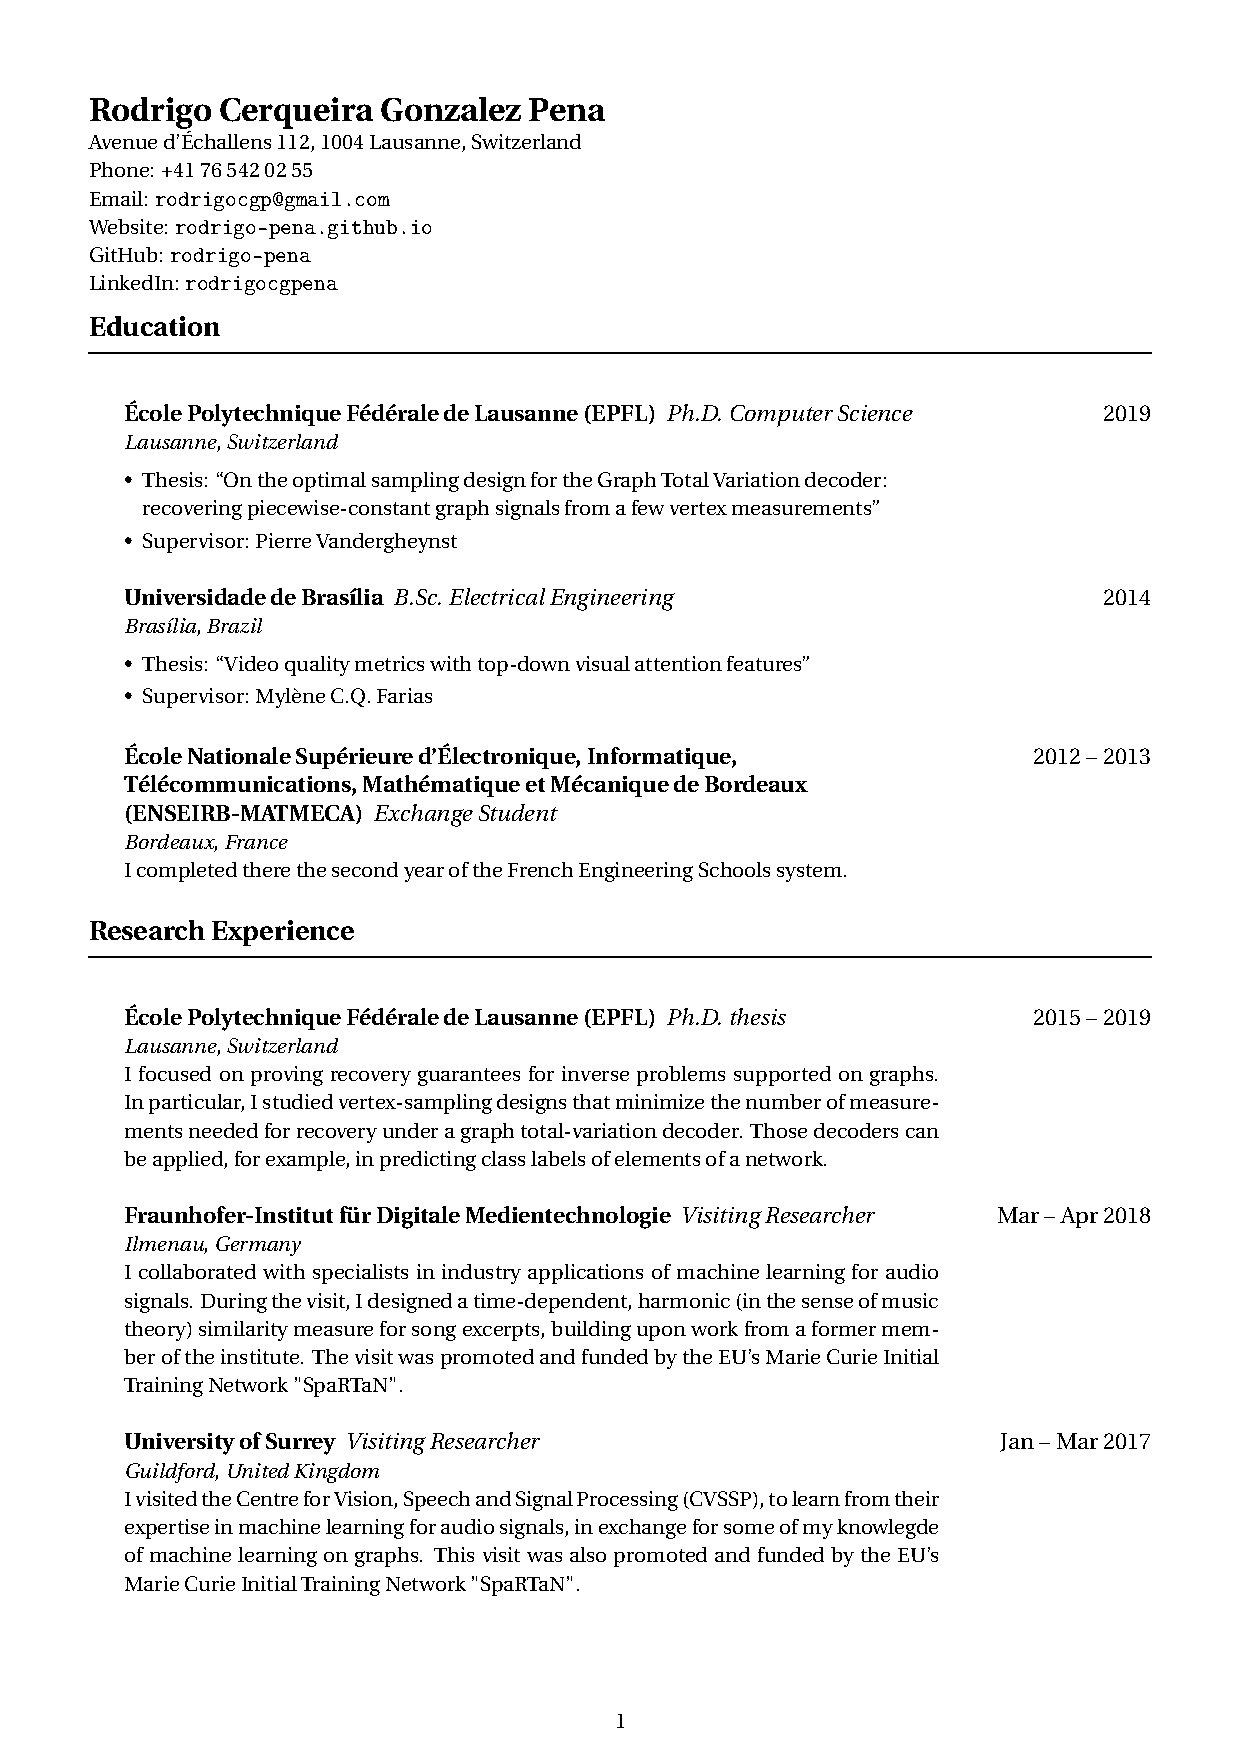
\includepdf[pagecommand=\thispagestyle{addpagenumbersforpdfimports},pages=-]{tail/cv.pdf}
% Links will not work in the included pdf, because pdflatex automatically "flattens" the file.


\end{document}
